\DocumentMetadata{%
  % uncompress, %only for debugging!!
  pdfversion=2.0,
  testphase={phase-II, tabular, graphic}%
  % testphase={phase-II,math, tabular, graphic}% TOC Does not work
  % testphase={phase-III,math}% TOC works
}
\tagpdfsetup{activate, tabsorder=structure}
% Use the following to fix bug in November 2023 download of LaTeX
\ExplSyntaxOn
\cs_generate_variant:Nn\__tag_prop_gput:Nnn{cnx}
\ExplSyntaxOff
\documentclass[11pt,
  english,
  letterpaper,
]{article}
\usepackage{sa4ss}
\usepackage{amsmath,amssymb,array}
\usepackage{booktabs}

% From tagged-template.latex
\usepackage{lmodern}
\usepackage{ifxetex,ifluatex}
\ifnum 0\ifxetex 1\fi\ifluatex 1\fi=0 % if pdftex
  \usepackage[T1]{fontenc}
  \usepackage[utf8]{inputenc}
  \usepackage{textcomp} % provide euro and other symbols
\else % if luatex or xetex
  \usepackage{unicode-math}
  \defaultfontfeatures{Scale=MatchLowercase}
  \defaultfontfeatures[\rmfamily]{Ligatures=TeX,Scale=1}
\fi

% Use upquote if available, for straight quotes in verbatim environments
\IfFileExists{upquote.sty}{\usepackage{upquote}}{}
\IfFileExists{microtype.sty}{% use microtype if available
  \usepackage[]{microtype}
  \UseMicrotypeSet[protrusion]{basicmath} % disable protrusion for tt fonts
}{}
\makeatletter
\@ifundefined{KOMAClassName}{% if non-KOMA class
  \IfFileExists{parskip.sty}{%
    \usepackage{parskip}
  }{% else
    \setlength{\parindent}{0pt}
    \setlength{\parskip}{6pt plus 2pt minus 1pt}}
}{% if KOMA class
  \KOMAoptions{parskip=half}}
\makeatother
\usepackage{xcolor}
\IfFileExists{xurl.sty}{\usepackage{xurl}}{} % add URL line breaks if available
\hypersetup{
  pdftitle={Status of Black Rockfish (Sebastes melanops) off Washington and federal waters in 2023},
  pdflang={en},
  hidelinks,
  pdfcreator={LaTeX via pandoc}}
\urlstyle{same} % disable monospaced font for URLs
\usepackage{longtable}
% Correct order of tables after \paragraph or \subparagraph
\usepackage{etoolbox}
\makeatletter
\patchcmd\longtable{\par}{\if@noskipsec\mbox{}\fi\par}{}{}
\makeatother
% Allow footnotes in longtable head/foot
\IfFileExists{footnotehyper.sty}{\usepackage{footnotehyper}}{\usepackage{footnote}}
\makesavenoteenv{longtable}
\usepackage{graphicx}
\makeatletter
\def\maxwidth{\ifdim\Gin@nat@width>\linewidth\linewidth\else\Gin@nat@width\fi}
\def\maxheight{\ifdim\Gin@nat@height>\textheight\textheight\else\Gin@nat@height\fi}
\makeatother
% Scale images if necessary, so that they will not overflow the page
% margins by default, and it is still possible to overwrite the defaults
% using explicit options in \includegraphics[width, height, ...]{}
\setkeys{Gin}{width=\maxwidth,height=\maxheight,keepaspectratio}
% Set default figure placement to htbp
\makeatletter
\def\fps@figure{htbp}
\makeatother
\setlength{\emergencystretch}{3em} % prevent overfull lines
\providecommand{\tightlist}{%
  \setlength{\itemsep}{0pt}\setlength{\parskip}{0pt}}
\setcounter{secnumdepth}{5}
\ifxetex
  % Load polyglossia as late as possible: uses bidi with RTL langages (e.g. Hebrew, Arabic)
  \usepackage{polyglossia}
  \setmainlanguage[]{}
\else
  \usepackage[shorthands=off,main=english]{babel}
\fi

%Define cslreferences environment, required by pandoc 2.8
%https://github.com/rstudio/rmarkdown/issues/1649
\newlength{\csllabelwidth}
\setlength{\csllabelwidth}{3em}
\newlength{\cslhangindent}
\setlength{\cslhangindent}{1.5em}
% for Pandoc 2.8 to 2.10.1
\newenvironment{cslreferences}%
  {}%
  {\par}
% For Pandoc 2.11+
\newenvironment{CSLReferences}[2] % #1 hanging-ident, #2 entry spacing
 {% don't indent paragraphs
  \setlength{\parindent}{0pt}
  % turn on hanging indent if param 1 is 1
  \ifodd #1 \everypar{\setlength{\hangindent}{\cslhangindent}}\ignorespaces\fi
  % set entry spacing
  \ifnum #2 > 0
  \setlength{\parskip}{#2\baselineskip}
  \fi
 }%
 {}
\usepackage{calc}  % for \widthof, \maxof in minipage
\newcommand{\CSLBlock}[1]{#1\hfill\break}
\newcommand{\CSLLeftMargin}[1]{\parbox[t]{\csllabelwidth}{#1}}
\newcommand{\CSLRightInline}[1]{\parbox[t]{\linewidth - \csllabelwidth}{#1}\break}
\newcommand{\CSLIndent}[1]{\hspace{\cslhangindent}#1}


\providecommand{\tightlist}{%
  \setlength{\itemsep}{0pt}\setlength{\parskip}{0pt}}


\date{}
\newcommand{\trTitle}{Status of Black Rockfish (\emph{Sebastes melanops}) off Washington and federal waters in 2023}
\newcommand{\trYear}{2023}
\newcommand{\trMonth}{June}
\newcommand{\trAuthsLong}{truetruetruetruetrue}
\newcommand{\trAuthsBack}{Cope, J.M., T.-. Tsou, L.K. Hillier, K.M. Hinton, C.B. Niles}
\newcommand{\trCitation}{
\begin{hangparas}{1em}{1}
\trAuthsBack{}. \trYear{}. \trTitle{}. \glsentrylong{pfmc}, Portland, Oregon. \pageref{LastPage}{}\,p.
\end{hangparas}}

\begin{document}

%%%%% Frontmatter %%%%%

% Footnote symbols in front matter
\renewcommand*{\thefootnote}{\fnsymbol{footnote}}

\small
\thispagestyle{empty}
\pagenumbering{roman}
\noindent
\begin{center}
\title{Status of Black Rockfish (\emph{Sebastes melanops}) off Washington and federal waters in 2023}
% \textnormal{\MakeTextUppercase{\trTitle{}}}
\vspace{1.5cm}
{\Large\textbf\newline{Status of Black Rockfish (\emph{Sebastes melanops}) off Washington and federal waters in 2023}}
\vfill
by\\
Jason M. Cope\textsuperscript{1}\\
Tien-Shui Tsou\textsuperscript{2}\\
Lisa K. Hillier\textsuperscript{2}\\
Kristen M. Hinton\textsuperscript{2}\\
Corey B. Niles\textsuperscript{2}\vfill
\textsuperscript{1}Northwest Fisheries Science Center, U.S. Department of Commerce, National Oceanic and Atmospheric Administration, National Marine Fisheries Service, 2725 Montlake Boulevard East, Seattle, Washington 98112\\
\textsuperscript{2}Washington Department of Fish and Wildlife, 600 Capital Way North, Olympia, Washington 98501\vfill
\trMonth{} \trYear{}
\end{center}
\clearpage

% Fourth page: Colophon
\thispagestyle{empty}
\vspace*{\fill}
\begin{center}
\copyright{} \glsentrylong{pfmc}, \trYear{}\\
\end{center}
\par
\bigskip
\noindent
Correct citation for this publication:
\bigskip
\par
\trCitation{}
\clearpage

% Add TOC to pdf bookmarks (clickable pdf)
\pdfbookmark[1]{\contentsname}{toc}

% Table of contents page, lists of figures and tables
\tableofcontents\clearpage
\label{TRlastRoman}
\clearpage

% Table of contents
\newpage
\thispagestyle{empty} % to remove page number

% Settings for the main document
\pagenumbering{arabic}  % Regular page numbers
\pagestyle{plain}  % No page number on first page of main document, use 'empty'
\renewcommand*{\thefootnote}{\arabic{footnote}}  % Back to numeric footnotes
\setcounter{footnote}{0}  % And start at 1
\renewcommand{\headrulewidth}{0.5pt}
\renewcommand{\footrulewidth}{0.5pt}
%\pagestyle{fancy}\fancyhead[c]{Draft: Do not cite or circulate}

\newcommand{\lt}{\ensuremath <}
\newcommand{\gt}{\ensuremath >}

\vspace{500cm}

\pagebreak
\pagenumbering{roman}
\setcounter{page}{1}

\renewcommand{\thetable}{\roman{table}}
\renewcommand{\thefigure}{\roman{figure}}

\setlength\parskip{0.5em plus 0.1em minus 0.2em}

\hypertarget{executive-summary}{%
\section*{Executive summary}\label{executive-summary}}
\addcontentsline{toc}{section}{Executive summary}

\hypertarget{stock}{%
\subsection*{Stock}\label{stock}}
\addcontentsline{toc}{subsection}{Stock}

This assessment reports the status of Black Rockfish (\emph{Sebastes melanops}) off Oregon state using data through 2022. Black Rockfish are also found in California (their core range) and Washington waters of the U.S. West Coast, and those are treated in separate area-based stock assessments given different mangement considerations and exploitation histories as discussed at the preliminary stock assessment workshop in February 2023 (Council 2023). There is substantial biogeographic separation in the populations off Oregon and Washington, thus justifying separation of those populations into different management units and stock assessments. Black Rockfish are also caught from the waters off British Columbia and Alaska, but there have not been any formal assessments of stock status for those areas. Genetic studies of stock structure indicate fish in Alaska are more differentiated than the along the contiguous west coast of the Unites States, and that genetic diversity varies in a nonsystematic way from California to Oregon (\textbf{Hessetal\_2023?}).

\hypertarget{removals}{%
\subsection*{Removals}\label{removals}}
\addcontentsline{toc}{subsection}{Removals}

Black Rockfish are caught by a wide variety of gear types in Oregon and in recent decades have been a very important target species for recreational charter-boats and private sport anglers (i.e., ocean boat fleet). In recent years the recreational fishery has accounted for most of the Black Rockfish catches (Figure \ref{fig:es-catch}). Black Rockfish can also be an important component of nearshore commercial fisheries, either as incidental catch by the troll fishery for salmon or as directed catch by jig fisheries for groundfish. Further, there are nearshore commercial fisheries that catch and sell fish live for the restaurant trade. There has been almost no trawl-caught landings of Black Rockfish in recent years (Table \ref{tab:removalsES}), but trawl landings in the 1940s to 1970s were more prominant (Figure \ref{fig:es-catch}).

Detailed reports of commercial landings of Black Rockfish are generally unavailable prior to 1981, when the Pacific Fishery Information Network (PacFIN) database began. The catch series prior to 1981 for these assessments were derived by applying available estimates or assumed values for the proportion of Black Rockfish landings in reported landings of rockfish. Observer data, which are available since the early 2000s, indicate low levels of discarding of Black Rockfish, generally less than 2\% of total catch. While Black Rockfish are unlikely to have ever comprised a large percentage of overall rockfish landings due to their low abundance compared to other rockfish species, it seems plausible that they have been more than a trivial component due to their nearshore distribution for many years. Black Rockfish were one of only four rockfish species mentioned by scientific name in reports of rockfish landings in Oregon during the 1940s.

Overall, removals of Black Rockfish remained relatively low (less than 100 mt) until the mid to late 1970s when landings quickly quadrupled with the expansion of the recreational fishery. Since the 1980s, removals have consistently fluctuated between 300 and 600 mt (no major trend), comprising mostly of removals from the ocean boat recreational fleet and the non-trawl commercial fleet (Figure \ref{fig:es-catch}).

\begingroup\fontsize{10}{12}\selectfont
\begingroup\fontsize{10}{12}\selectfont

\begin{longtable}[t]{r>{\centering\arraybackslash}p{2.2cm}>{\centering\arraybackslash}p{2.2cm}>{\centering\arraybackslash}p{2.2cm}>{\centering\arraybackslash}p{2.2cm}}
\caption{\label{tab:removalsES}Recent catches (mt) by fleet and total catch (mt) summed across fleets for the  model area.}\\
\toprule
Year & Trawl (mt) & NonTRWL (mt) & Recreational (mt) & Total Catch (mt)\\
\midrule
\endfirsthead
\caption[]{Recent catches (mt) by fleet and total catch (mt) summed across fleets for the  model area. \textit{(continued)}}\\
\toprule
Year & Trawl (mt) & NonTRWL (mt) & Recreational (mt) & Total Catch (mt)\\
\midrule
\endhead

\endfoot
\bottomrule
\endlastfoot
2013 & 0.08 & 0.00 & 325.94 & 326.02\\
2014 & 0.99 & 0.01 & 355.96 & 356.96\\
2015 & 0.95 & 1.38 & 361.11 & 363.44\\
2016 & 0.50 & 0.23 & 368.66 & 369.39\\
2017 & 0.24 & 1.19 & 239.59 & 241.02\\
2018 & 0.03 & 1.85 & 262.91 & 264.79\\
2019 & 0.01 & 1.88 & 249.20 & 251.09\\
2020 & 0.05 & 1.92 & 128.39 & 130.36\\
2021 & 0.01 & 0.64 & 197.04 & 197.68\\
2022 & 0.00 & 1.12 & 164.93 & 166.05\\*
\end{longtable}
\endgroup{}
\endgroup{}


\begin{figure}
\centering
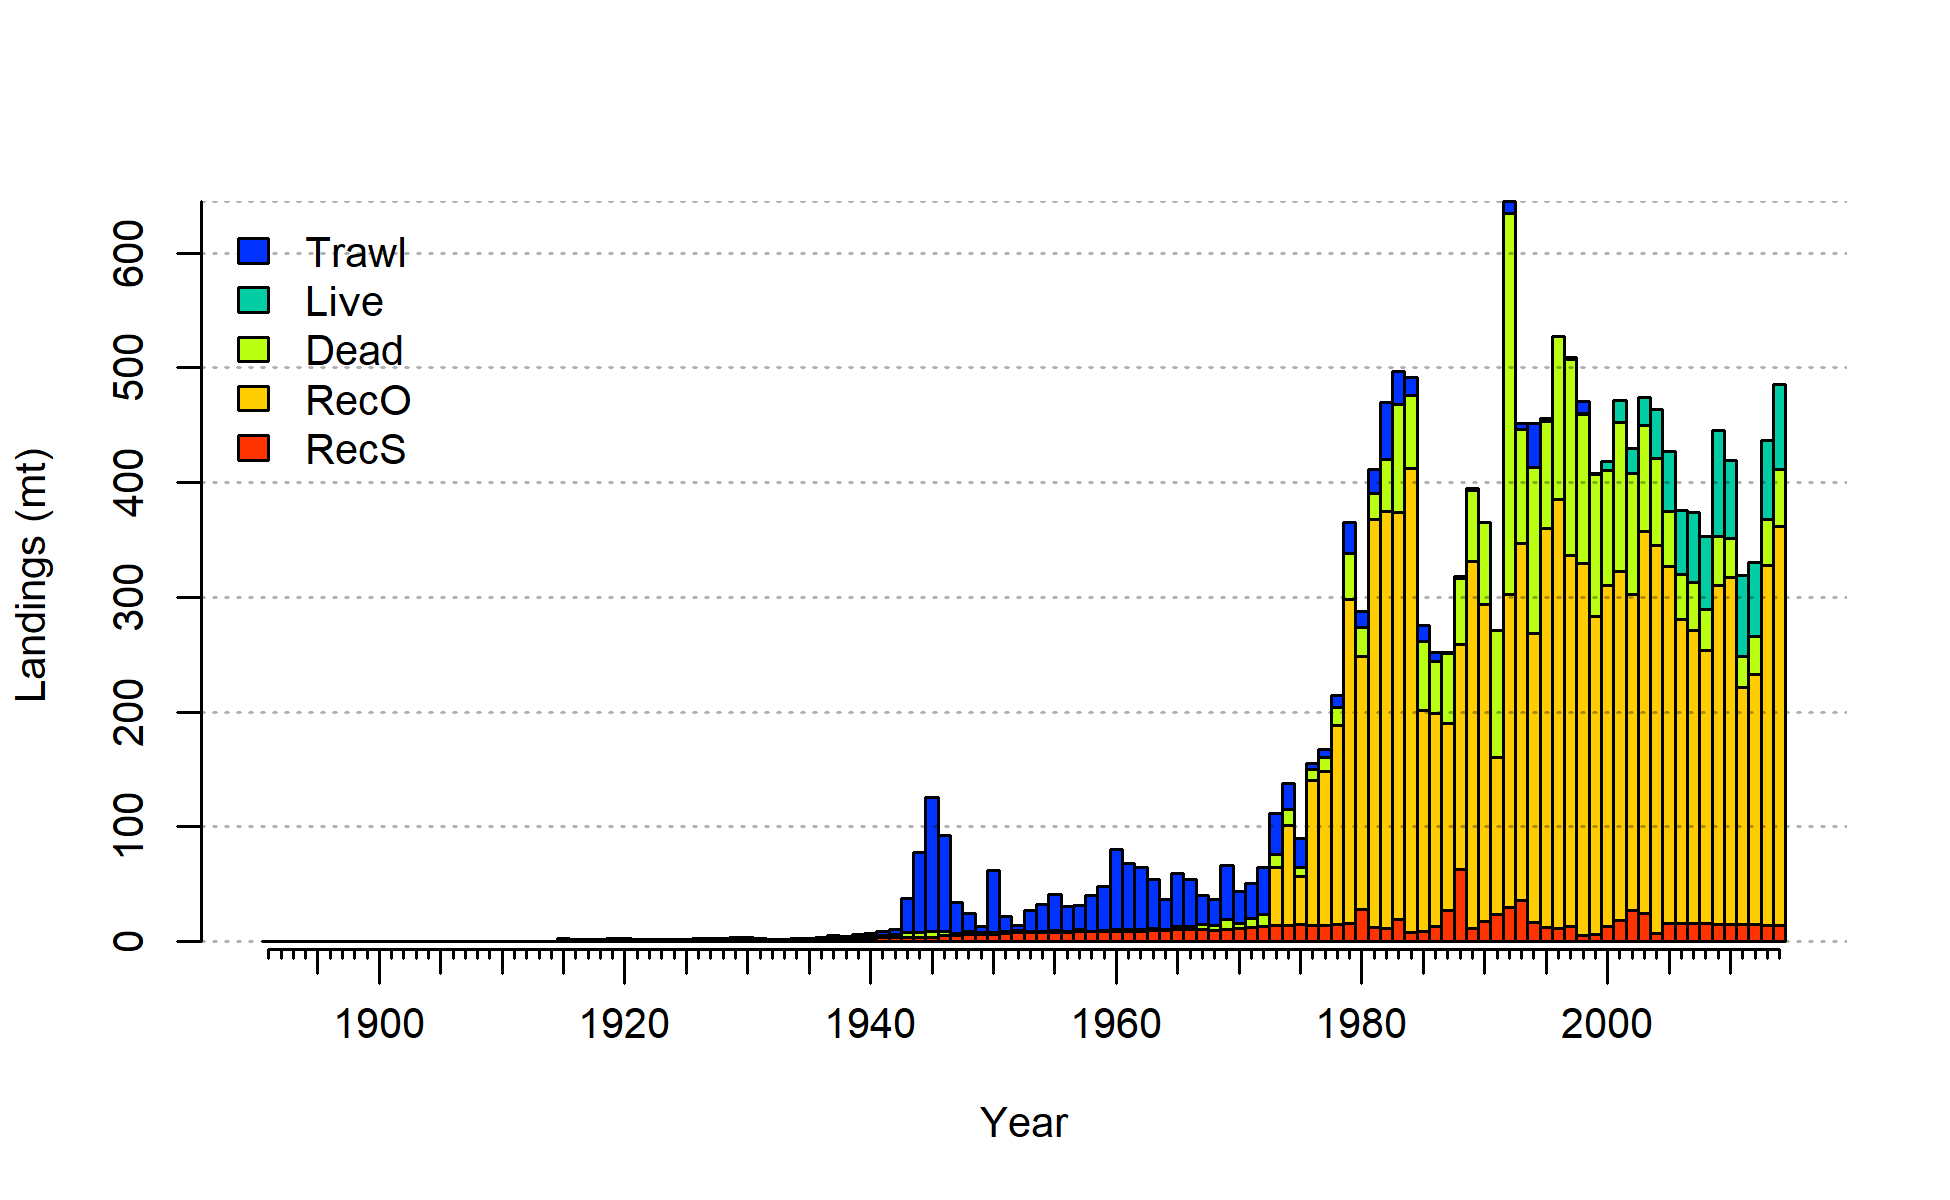
\includegraphics[width=1\textwidth,height=1\textheight]{C:/Users/Jason.Cope/Documents/Github/Sebastes_melanops_WA/Document/models/Reference model/plots/catch2 landings stacked.png}
\caption{Landings by fleet used in the reference model where catches in metric tons by fleet are stacked.\label{fig:es-catch}}
\end{figure}

\clearpage

\hypertarget{data-and-assessment}{%
\subsection*{Data and assessment}\label{data-and-assessment}}
\addcontentsline{toc}{subsection}{Data and assessment}

The first Black Rockfish stock assessment along the west coast of the United States that included the majority of Oregon waters was completed in 2007, covering the area south of Cape Falcon, Oregon to north of Point Piedros Blancos, California (Sampson 2007). In 2015, a subsequent assessment was completed that included Oregon waters only as one of three (also Washington and California) seperate assessment areas delineated by state lines (J. M. Cope et al. 2016). Similarly, this assessment treats Oregon waters as a single assessment area. The previous two assessments used Stock Synthesis software, as does this one (version 3.30.21.00).

This assessment integrates data and information from multiple sources into one modeling framework. The stock assessment model for Black Rockfish is informed by catch data from two commercial fleets and two recreational fleets, six abundance indices, five sets of length composition data, and 3 sets of conditional age-at-length compositions. It also uses an ageing error matrix to incorporate ageing imprecision and applies fixed parameterizations of weight-at-length, maturity-at-length, fecundity-at-length, the Beverton-Holt stock-recruitment steepness value, and recruitment variability. Life history parameters were sex-specific (i.e., a two-sex model) with natural mortality fixed at external estimates and growth and recruitment parameters estimated. Additional parameters that were estimated include initial population scale (\(lnR_0\)), selectivity for each fishery and survey, and extra survey variance. The base model was tuned to account for the weighting of the length and age data and index variances (which was estimated), as well as the specification of the recruitment bias adjustments. Derived quantities include, among other things, the time series of spawning biomass, age and size structure, and current and projected future stock status. The model covers the years 1940 to 2022, with a 12 year forecast beginning in 2023.

Within model uncertainty is explicitly included in this assessment by parameter estimation uncertainty, while among model uncertainty is explored through sensitivity analyses addressing alternative input assumptions such as data treatment and weighting, and model specification sensitivity to the treatment of life history parameters, selectivity, recruitment, and survey catchability. A reference model was selected that best fit the observed data while concomitantly balancing the desire to capture the central tendency across those sources of uncertainty, ensure model realism and tractability, and promote robustness to potential model misspecification.

\hypertarget{stock-biomass-and-dynamics}{%
\subsection*{Stock biomass and dynamics}\label{stock-biomass-and-dynamics}}
\addcontentsline{toc}{subsection}{Stock biomass and dynamics}

Spawning output (in millions of eggs; meggs) instead of spawning biomass is used to report the functionally mature population scale because fecundity is nonlinearly related to body female weight. The estimated spawning output at the beginning of 2023 was 465 meggs (\textasciitilde95 percent asymptotic intervals: 281 to 650 meggs, Table \ref{tab:ssbES} and Figure \ref{fig:es-ssb}), which when compared to unfished spawning output (957) meggs gives a relative stock status level of 49 percent (\textasciitilde95 percent asymptotic intervals: 33 to 64 percent, Figure \ref{fig:es-depl}). Overall, spawning output declined with the onset of increasing commercial removals in the 1960s and continued to decline with the increase in recreational catches through the 1990s, even dropping below the target relative stock size from 1993 to 2008, before steadily increasing back above target since that time. The largest of the estimated recruitment pulses occurred in 2008 and was followed by several above average recruitment years in the early 2010s, which contributed to the increase in spawning output through the mid to late 2010s. The minimum relative stock size of 17 percent of unfished levels is estimated to have occurred in 1995. Accordingly, the stock has not been below the minimum stock size threshold (i.e., never overfished based on median estimates). Currently the stock is estimated above the management target of \(SO_{40\%}\) in 2023 and is estimated to have remained above the target since 2009 (Table \ref{tab:ssbES} and Figure \ref{fig:es-depl}).

\begingroup\fontsize{10}{12}\selectfont
\begingroup\fontsize{10}{12}\selectfont

\begin{longtable}[t]{r>{\centering\arraybackslash}p{1.57cm}>{\centering\arraybackslash}p{1.57cm}>{\centering\arraybackslash}p{1.57cm}>{\centering\arraybackslash}p{1.57cm}>{\centering\arraybackslash}p{1.57cm}>{\centering\arraybackslash}p{1.57cm}}
\caption{\label{tab:ssbES}Estimated recent trend in spawning output and the fraction unfished and the 95 percent intervals.}\\
\toprule
Year & Spawning Output & Lower Interval & Upper Interval & Fraction Unfished & Lower Interval & Upper Interval\\
\midrule
\endfirsthead
\caption[]{Estimated recent trend in spawning output and the fraction unfished and the 95 percent intervals. \textit{(continued)}}\\
\toprule
Year & Spawning Output & Lower Interval & Upper Interval & Fraction Unfished & Lower Interval & Upper Interval\\
\midrule
\endhead

\endfoot
\bottomrule
\endlastfoot
2013 & 239.61 & 189.29 & 289.93 & 0.25 & 0.21 & 0.29\\
2014 & 249.53 & 192.38 & 306.68 & 0.26 & 0.22 & 0.31\\
2015 & 261.05 & 195.22 & 326.88 & 0.27 & 0.22 & 0.33\\
2016 & 274.76 & 198.39 & 351.13 & 0.29 & 0.23 & 0.35\\
2017 & 289.73 & 200.98 & 378.47 & 0.31 & 0.23 & 0.38\\
2018 & 319.12 & 216.03 & 422.21 & 0.34 & 0.25 & 0.42\\
2019 & 346.49 & 227.88 & 465.10 & 0.36 & 0.27 & 0.46\\
2020 & 372.63 & 238.20 & 507.06 & 0.39 & 0.28 & 0.51\\
2021 & 406.97 & 257.39 & 556.55 & 0.43 & 0.30 & 0.56\\
2022 & 425.64 & 263.13 & 588.16 & 0.45 & 0.31 & 0.59\\
2023 & 439.55 & 266.93 & 612.16 & 0.46 & 0.31 & 0.61\\*
\end{longtable}
\endgroup{}
\endgroup{}


\begin{figure}
\centering
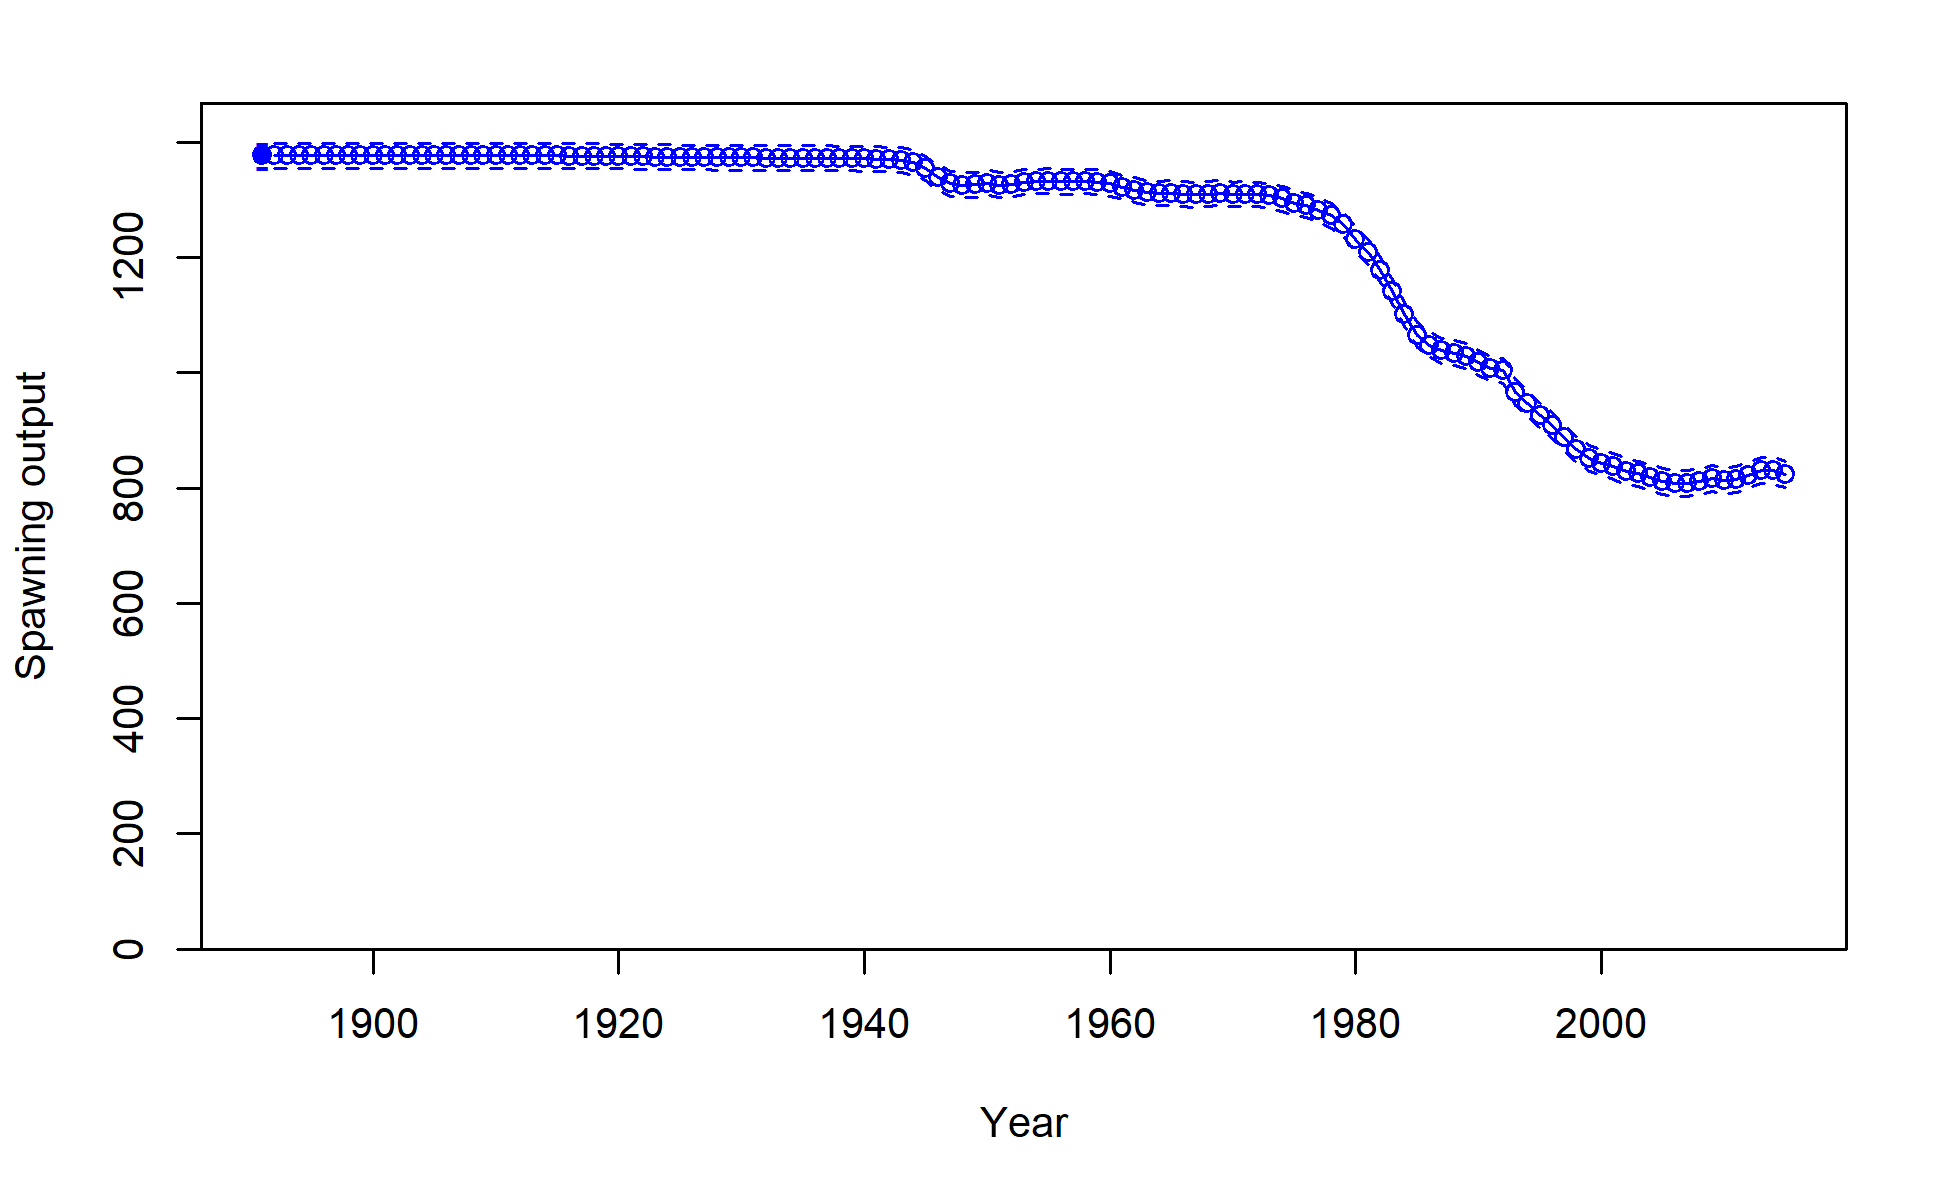
\includegraphics[width=1\textwidth,height=1\textheight]{C:/Users/Jason.Cope/Documents/Github/Sebastes_melanops_WA/Document/models/Reference model/plots/ts7_Spawning_output_with_95_asymptotic_intervals_intervals.png}
\caption{Estimated time series of spawning output (circles and line: median; light broken lines: 95 percent intervals) for the base model.\label{fig:es-ssb}}
\end{figure}

\begin{figure}
\centering
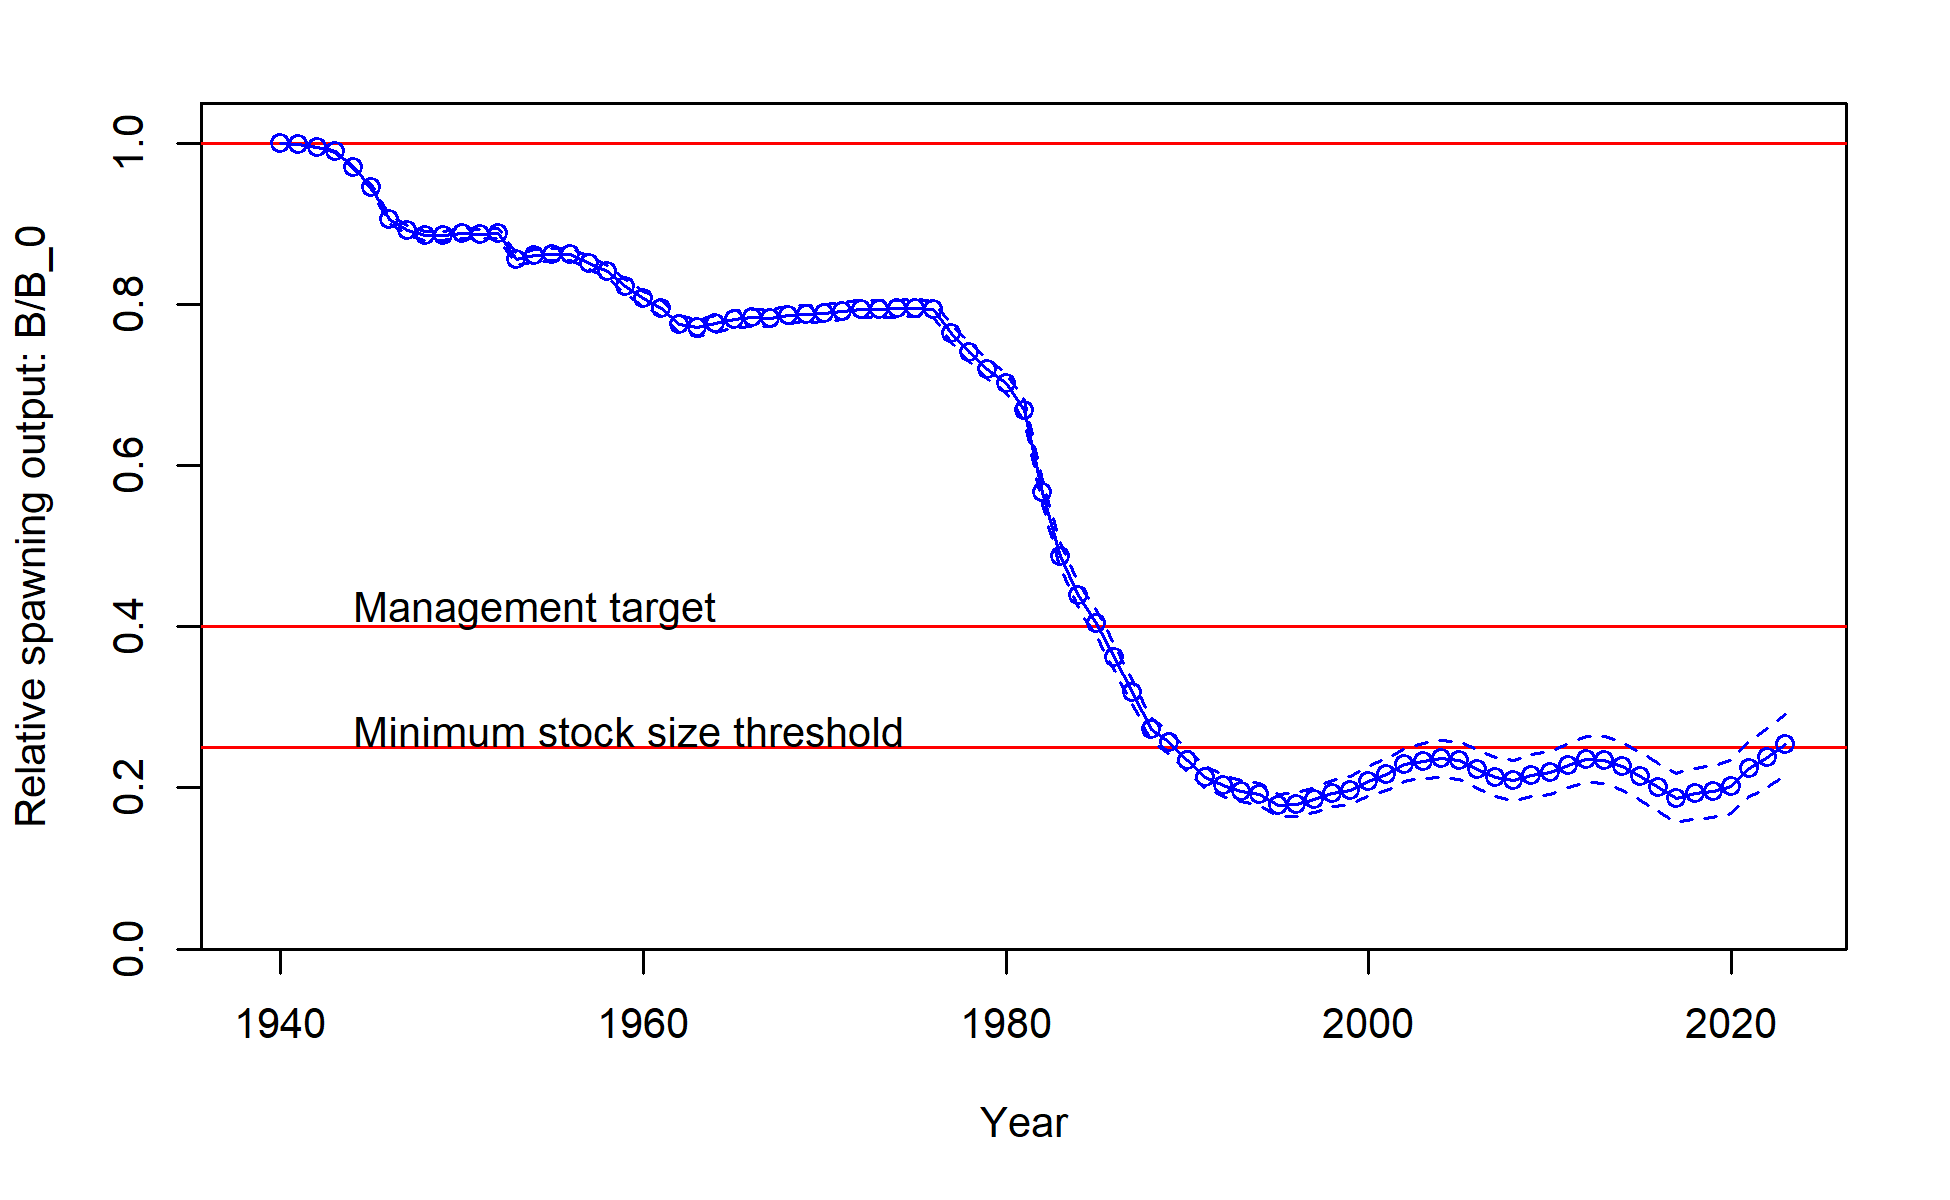
\includegraphics[width=1\textwidth,height=1\textheight]{C:/Users/Jason.Cope/Documents/Github/Sebastes_melanops_WA/Document/models/Reference model/plots/ts9_Relative_spawning_output_intervals.png}
\caption{Estimated time series of fraction of unfished spawning output (circles and line: median; light broken lines: 95 percent intervals) for the base model.\label{fig:es-depl}}
\end{figure}

\clearpage

\hypertarget{recruitment}{%
\subsection*{Recruitment}\label{recruitment}}
\addcontentsline{toc}{subsection}{Recruitment}

Recruitment is informed by the data from 1980 to 2017 (Table \ref{tab:recrES} and Figure \ref{fig:es-recruits}). The highest recruitment years occurred in 1999, 2000, 2008, 2013, and 2016. The large 2008 and 2016 year classes, as well as several above average year classes in the early 2010s, contributed to the recent increase in Black Rockfish biomass. Recruitment is informed by composition data and six relative abundance indices. The 2015 stock assessment did not estimate deviations from the stock-recruitment curve. While the Black Rockfish stock has been reduced to levels that theoretically would provide some information on how recruitment compensation changes across spawning biomass levels (i.e., inform the steepness parameter), the assessment model could not adequately estimate a reasonable steepness parameter. Thus, recruitment is based on a fixed assumption about steepness (\(h\) = 0.72) and recruitment variability (\(\sigma_R\) = 0.6).

\begingroup\fontsize{10}{12}\selectfont
\begingroup\fontsize{10}{12}\selectfont

\begin{longtable}[t]{r>{\centering\arraybackslash}p{1.57cm}>{\centering\arraybackslash}p{1.57cm}>{\centering\arraybackslash}p{1.57cm}>{\centering\arraybackslash}p{1.57cm}>{\centering\arraybackslash}p{1.57cm}>{\centering\arraybackslash}p{1.57cm}}
\caption{\label{tab:recrES}Estimated recent trend in recruitment and recruitment deviations and the 95 percent intervals.}\\
\toprule
Year & Recruitment & Lower Interval & Upper Interval & Recruitment Deviations & Lower Interval & Upper Interval\\
\midrule
\endfirsthead
\caption[]{Estimated recent trend in recruitment and recruitment deviations and the 95 percent intervals. \textit{(continued)}}\\
\toprule
Year & Recruitment & Lower Interval & Upper Interval & Recruitment Deviations & Lower Interval & Upper Interval\\
\midrule
\endhead

\endfoot
\bottomrule
\endlastfoot
2013 & 1972.96 & 1304.38 & 2984.22 & 0.42 & 0.08 & 0.77\\
2014 & 1524.90 & 970.90 & 2395.02 & 0.15 & -0.23 & 0.54\\
2015 & 1117.78 & 678.00 & 1842.81 & -0.17 & -0.61 & 0.27\\
2016 & 1222.12 & 732.14 & 2040.03 & -0.12 & -0.57 & 0.34\\
2017 & 745.60 & 383.36 & 1450.13 & -0.65 & -1.28 & -0.02\\
2018 & 1640.14 & 1429.19 & 1882.23 & 0.00 & 0.00 & 0.00\\
2019 & 1671.35 & 1454.43 & 1920.62 & 0.00 & 0.00 & 0.00\\
2020 & 1697.60 & 1475.50 & 1953.13 & 0.00 & 0.00 & 0.00\\
2021 & 1728.44 & 1505.90 & 1983.87 & 0.00 & 0.00 & 0.00\\
2022 & 1742.76 & 1516.49 & 2002.79 & 0.00 & 0.00 & 0.00\\
2023 & 1752.52 & 1523.38 & 2016.13 & 0.00 & 0.00 & 0.00\\*
\end{longtable}
\endgroup{}
\endgroup{}


\begin{figure}
\centering
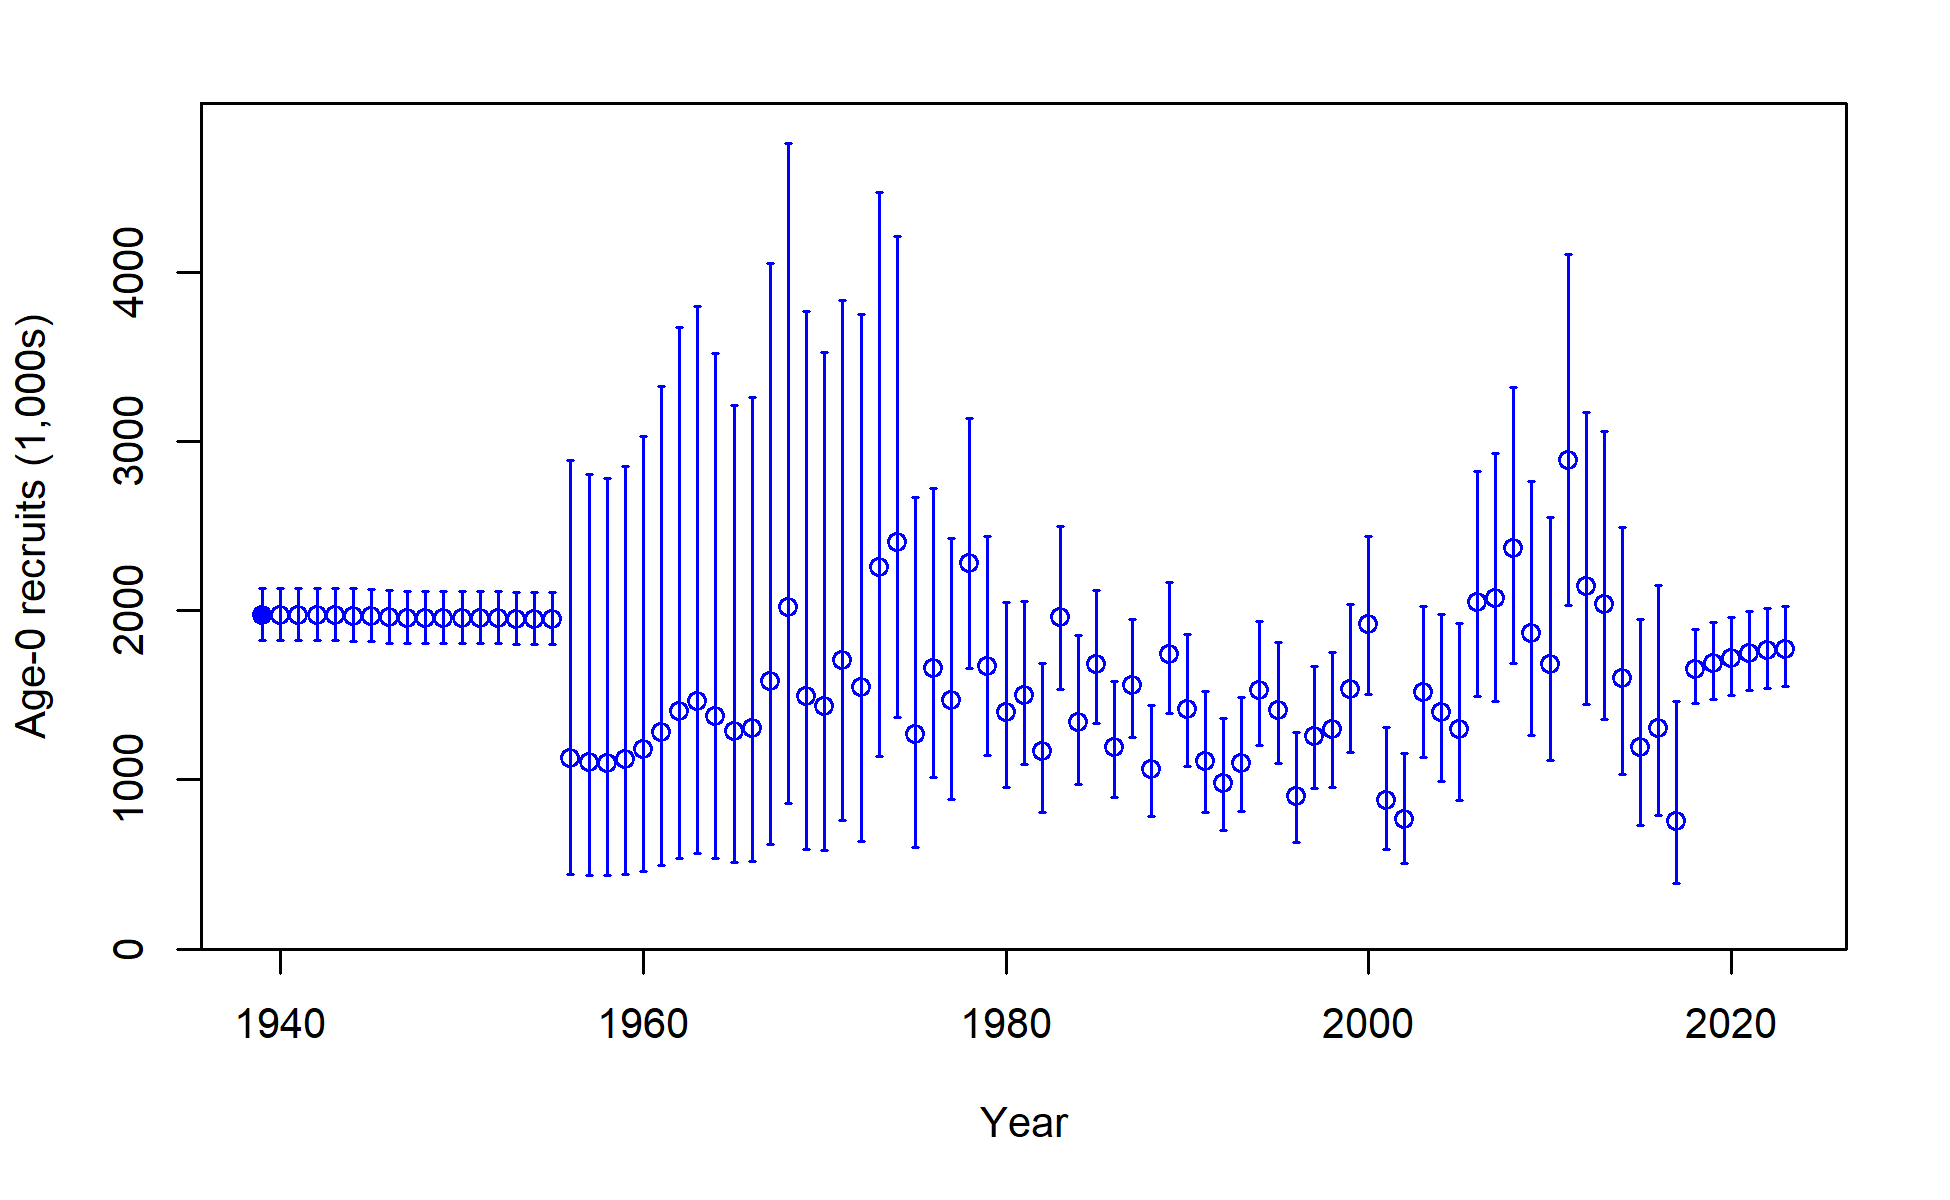
\includegraphics[width=1\textwidth,height=1\textheight]{C:/Users/Jason.Cope/Documents/Github/Sebastes_melanops_WA/Document/models/Reference model/plots/ts11_Age-0_recruits_(1000s)_with_95_asymptotic_intervals.png}
\caption{Estimated time series of age-0 recruits (1000s) for the base model with 95 percent intervals.\label{fig:es-recruits}}
\end{figure}

\begin{figure}
\centering
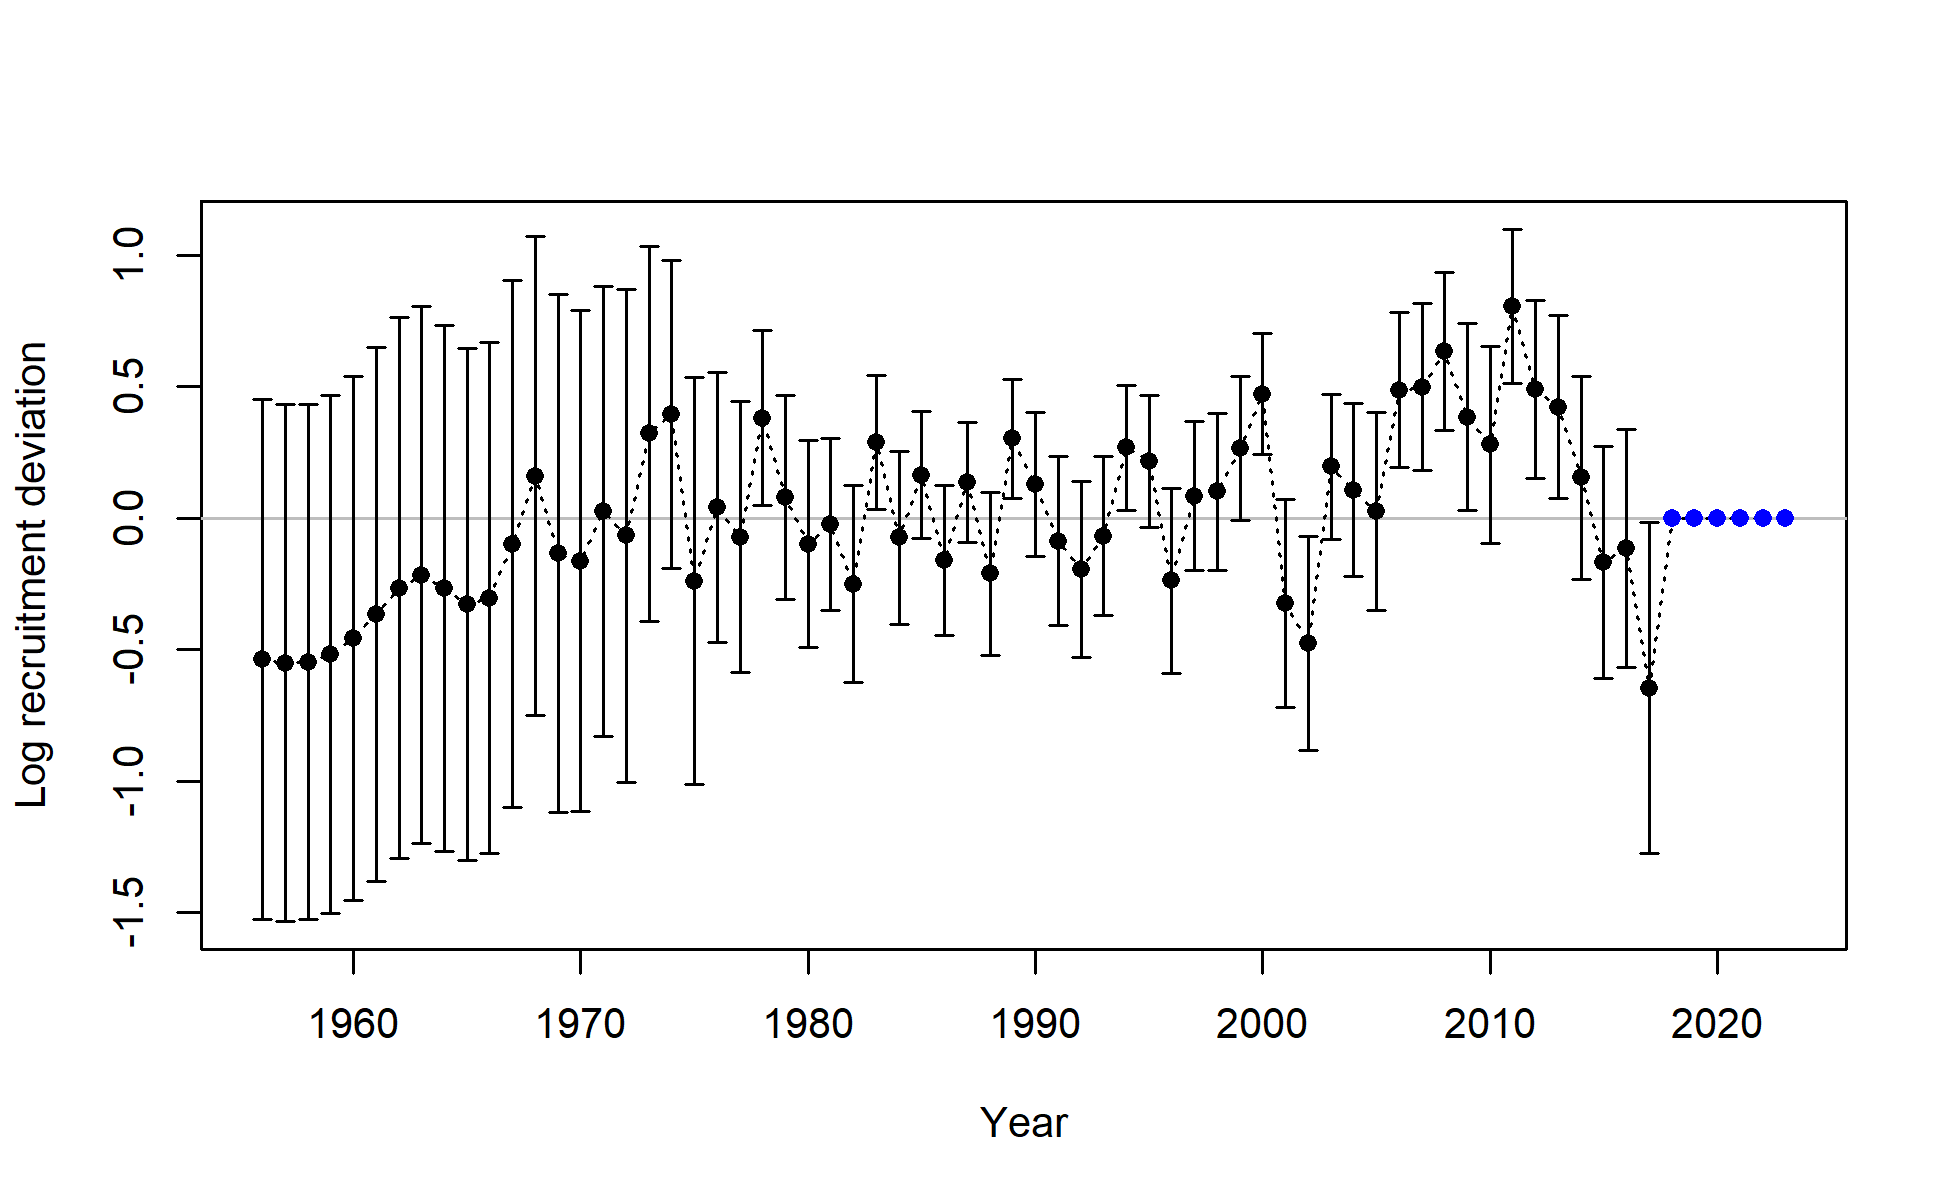
\includegraphics[width=1\textwidth,height=1\textheight]{C:/Users/Jason.Cope/Documents/Github/Sebastes_melanops_WA/Document/models/Reference model/plots/recdevs2_withbars.png}
\caption{Estimated time series of recruitment deviations.\label{fig:es-recdev}}
\end{figure}

\hypertarget{exploitation-status}\)) since 1980. Fishing was at or above the target rate from 1989 to 2005 and has been slightly below it over the past 5 years (Table \ref{tab:exploitES} and Figures \ref{fig:es-1-spr} and \ref{fig:es-phase}). The steepness value of 0.72 indicates that a lower value of SPR (or equivalently a higher fishing intensity than \(\text{SPR}_{50\%}\)) would be consistent with the biomass-based target of (\(\text{SO}_{40\%}\)) for sustainable removals. Trends in fishing intensity largely mirrored that of landings until the 1990s, after which recruitment pulses countered the catches somewhat to lower overall fishing intensity (Figure \ref{fig:es-1-spr}). The maximum fishing intensity was 0.8 in 1994, which is well above the target SPR-based harvest rate of 0.50. The current level of 0.39 for 2022 is below that target. Fishing intensity over the past decade has ranged between 0.3 and 0.65 and the exploitation rate (range of 0.02 - 0.07, Table \ref{tab:exploitES}) has come down since the time series high of 0.12 in 1992. Current estimates indicate that Black Rockfish spawning output is greater than than the target biomass level (\(\text{SO}_{40\%}\)), though fishing intensity remains near the target \(F_{MSY}\) proxy harvest rate of 1 - \(\text{SPR}_{50\%}\) (Figure \ref{fig:es-phase}).

\begingroup\fontsize{10}{12}\selectfont
\begingroup\fontsize{10}{12}\selectfont

\begin{longtable}[t]{r>{\centering\arraybackslash}p{1.57cm}>{\centering\arraybackslash}p{1.57cm}>{\centering\arraybackslash}p{1.57cm}>{\centering\arraybackslash}p{1.57cm}>{\centering\arraybackslash}p{1.57cm}>{\centering\arraybackslash}p{1.57cm}}
\caption{\label{tab:exploitES}Estimated recent trend in the 1-SPR where SPR is the spawning potential ratio the exploitation rate, and the  95 percent intervals.}\\
\toprule
Year & 1-SPR & Lower Interval & Upper Interval & Exploitation Rate & Lower Interval & Upper Interval\\
\midrule
\endfirsthead
\caption[]{Estimated recent trend in the 1-SPR where SPR is the spawning potential ratio the exploitation rate, and the  95 percent intervals. \textit{(continued)}}\\
\toprule
Year & 1-SPR & Lower Interval & Upper Interval & Exploitation Rate & Lower Interval & Upper Interval\\
\midrule
\endhead

\endfoot
\bottomrule
\endlastfoot
2013 & 0.65 & 0.60 & 0.71 & 0.06 & 0.05 & 0.08\\
2014 & 0.67 & 0.60 & 0.73 & 0.07 & 0.05 & 0.08\\
2015 & 0.66 & 0.59 & 0.73 & 0.07 & 0.05 & 0.09\\
2016 & 0.65 & 0.57 & 0.73 & 0.07 & 0.05 & 0.09\\
2017 & 0.52 & 0.43 & 0.61 & 0.05 & 0.03 & 0.06\\
2018 & 0.53 & 0.43 & 0.62 & 0.05 & 0.03 & 0.07\\
2019 & 0.50 & 0.40 & 0.59 & 0.05 & 0.03 & 0.07\\
2020 & 0.32 & 0.23 & 0.40 & 0.03 & 0.02 & 0.03\\
2021 & 0.41 & 0.31 & 0.51 & 0.04 & 0.03 & 0.05\\
2022 & 0.37 & 0.27 & 0.46 & 0.03 & 0.02 & 0.04\\*
\end{longtable}
\endgroup{}
\endgroup{}


\begin{figure}
\centering
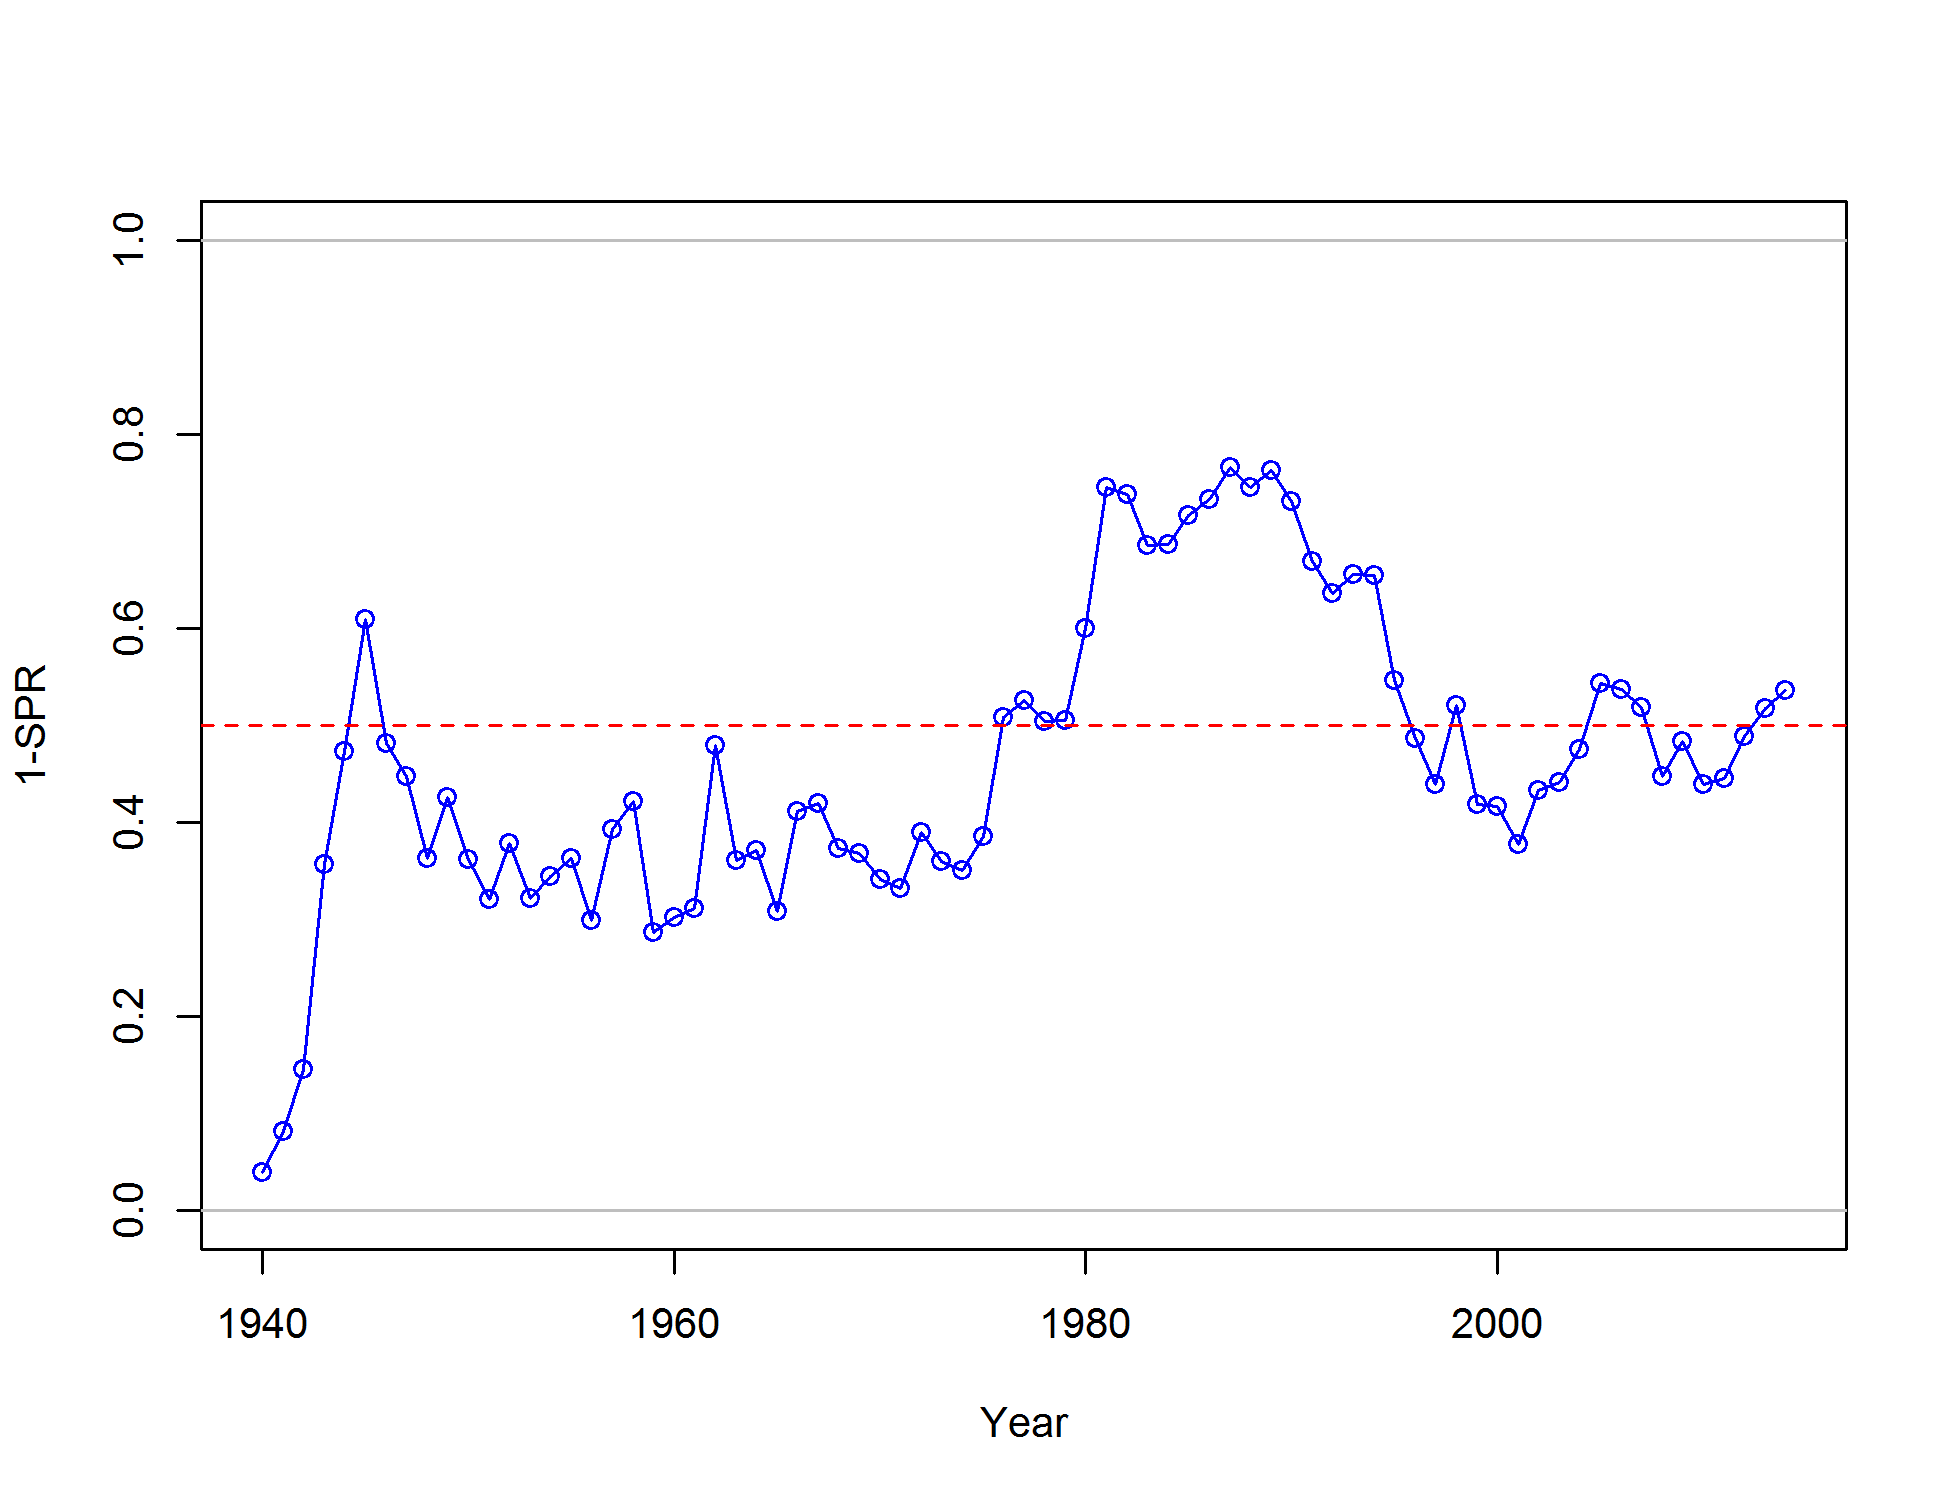
\includegraphics[width=1\textwidth,height=1\textheight]{C:/Users/Jason.Cope/Documents/Github/Sebastes_melanops_WA/Document/models/Reference model/plots/SPR2_minusSPRseries.png}
\caption{Estimated 1 - relative spawning ratio (SPR) by year for the base model. The management target is plotted as a red horizontal line and values above this reflect harvest in excess of the proxy harvest rate.\label{fig:es-1-spr}}
\end{figure}

\clearpage

\hypertarget{ecosystem-considerations}{%
\subsection*{Ecosystem considerations}\label{ecosystem-considerations}}
\addcontentsline{toc}{subsection}{Ecosystem considerations}

This stock assessment does not explicitly incorporate trophic interactions, habitat factors or environmental factors into the assessment model. More predation, diet and habitat work, and mechanistic linkages to environmental conditions would be needed to incorporate these elements into the stock assessment and should remain a priority. McClure et al. (2023) report the climate vulnerability for several west coast groundfishes, including Black Rockfish. Black Rockfish demonstrated both high biological sensitivity and high climate exposure risk, to give it an overall high vulnerability score to climate change. This result should also be considered with the fact that like many rockfishes, periods of low productivity is not unusually to Black Rockfish and their extended longevity has historically allowed them to wait for advantageous productivity periods. Additional stressors such as fishing and climate change that possibly truncate longevity could bring significant challenges to population sustainability.

\hypertarget{reference-points}\)), target relative biomass (40\%), and estimated selectivity and catch for each fleet (Table \ref{tab:referenceES}). The Black Rockfish population in Oregon at the start of 2023 is estimated to be 1.38 times (above) the target biomass, and fishing intensity during 2022 is estiamted to be 0.96 times (below) the fishing intensity target (Figure \ref{fig:es-phase}). The yield values are lower than the previous assessment for similar reference points due to updated life history estimates. The proxy MSY values of management quantities are the most conservative compared to the estimated MSY and MSY relative to 40\% biomass. Sustainable total yield, removals, using the proxy \(\text{SPR}_{50\%}\) is 280 mt. The spawning output equivalent to 40 percent of the unfished spawning output (\(\text{SO}_{40\%}\)) calculated using the SPR target (\(\text{SPR}_{50\%}\)) was 427 meggs.

Recent removals have been close to the point estimate of potential long-term yields calculated using an \(\text{SPR}_{50\%}\) reference point, though the population size has continued to increase over recent years due to several above average recruitments. The equilibrium estimates of yield relative to biomass based on a steepness value fixed at 0.72 are provided in Figure \ref{fig:es-yield}, where vertical dashed lines indicate the estimate of fraction unfished at the start of 2023 (current) and the estimated management targets calculated based on the relative target biomass (B target), the SPR target, and the maximum sustainable yield (MSY).

The 2023 spawning biomass relative to unfished equilibrium spawning biomass, based on the 2022 fishing year, is above (55 percent) the management target of 40 percent of unfished spawning output. The relative biomass and the ratio of the estimated SPR to the management target (\(\text{SPR}_{50\%}\)) across all model years are shown in Figure \ref{fig:es-phase} where warmer colors (red) represent early years and colder colors (blue) represent recent years. There have been periods where the stock status has decreased below the target and fishing intensity has been higher than the target fishing intensity based on \(\text{SPR}_{50\%}\).

\begin{figure}
\centering
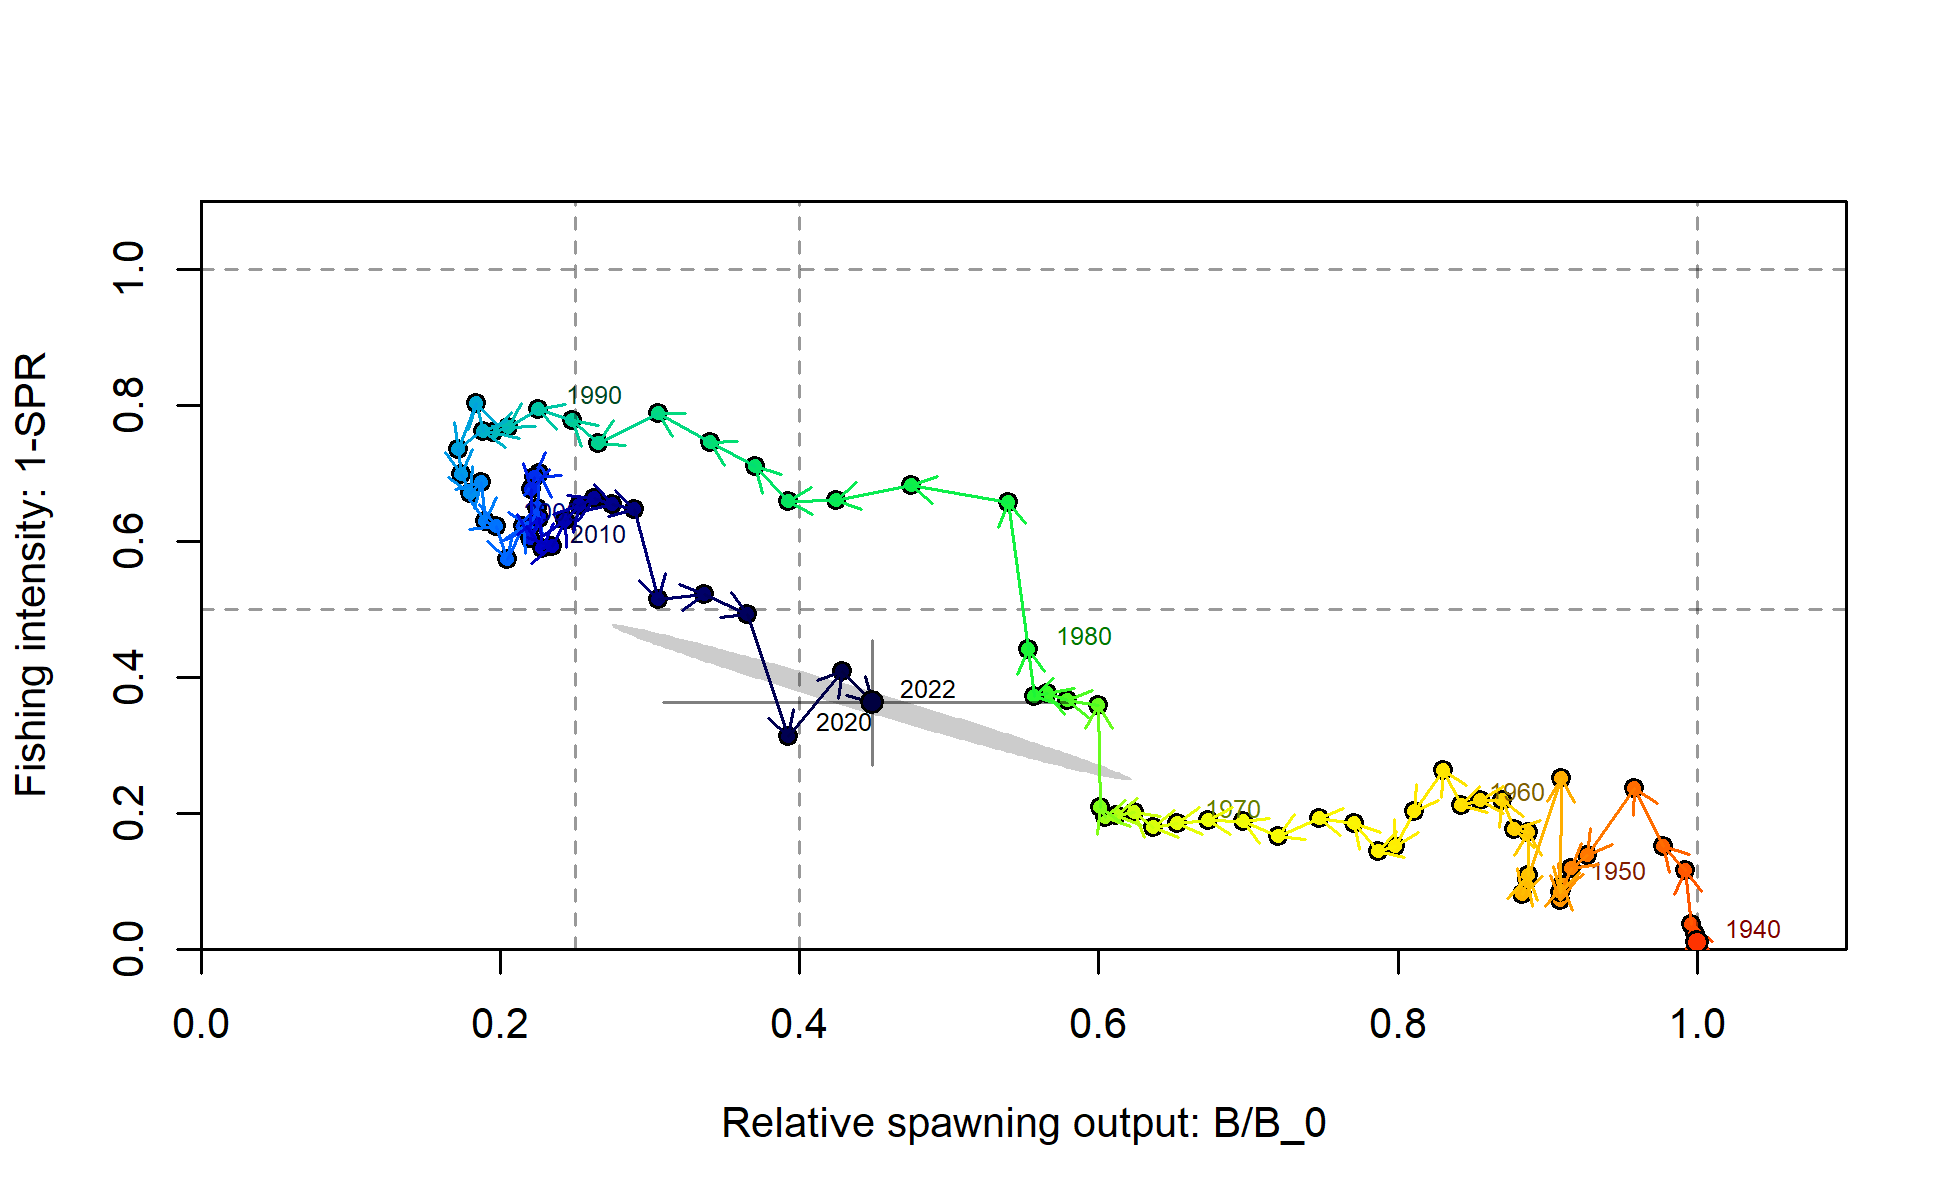
\includegraphics[width=1\textwidth,height=1\textheight]{C:/Users/Jason.Cope/Documents/Github/Sebastes_melanops_WA/Document/models/Reference model/plots/SPR4_phase.png}
\caption{Phase plot of estimated 1-SPR versus fraction unfished for the base model.\label{fig:es-phase}}
\end{figure}

\begin{figure}
\centering
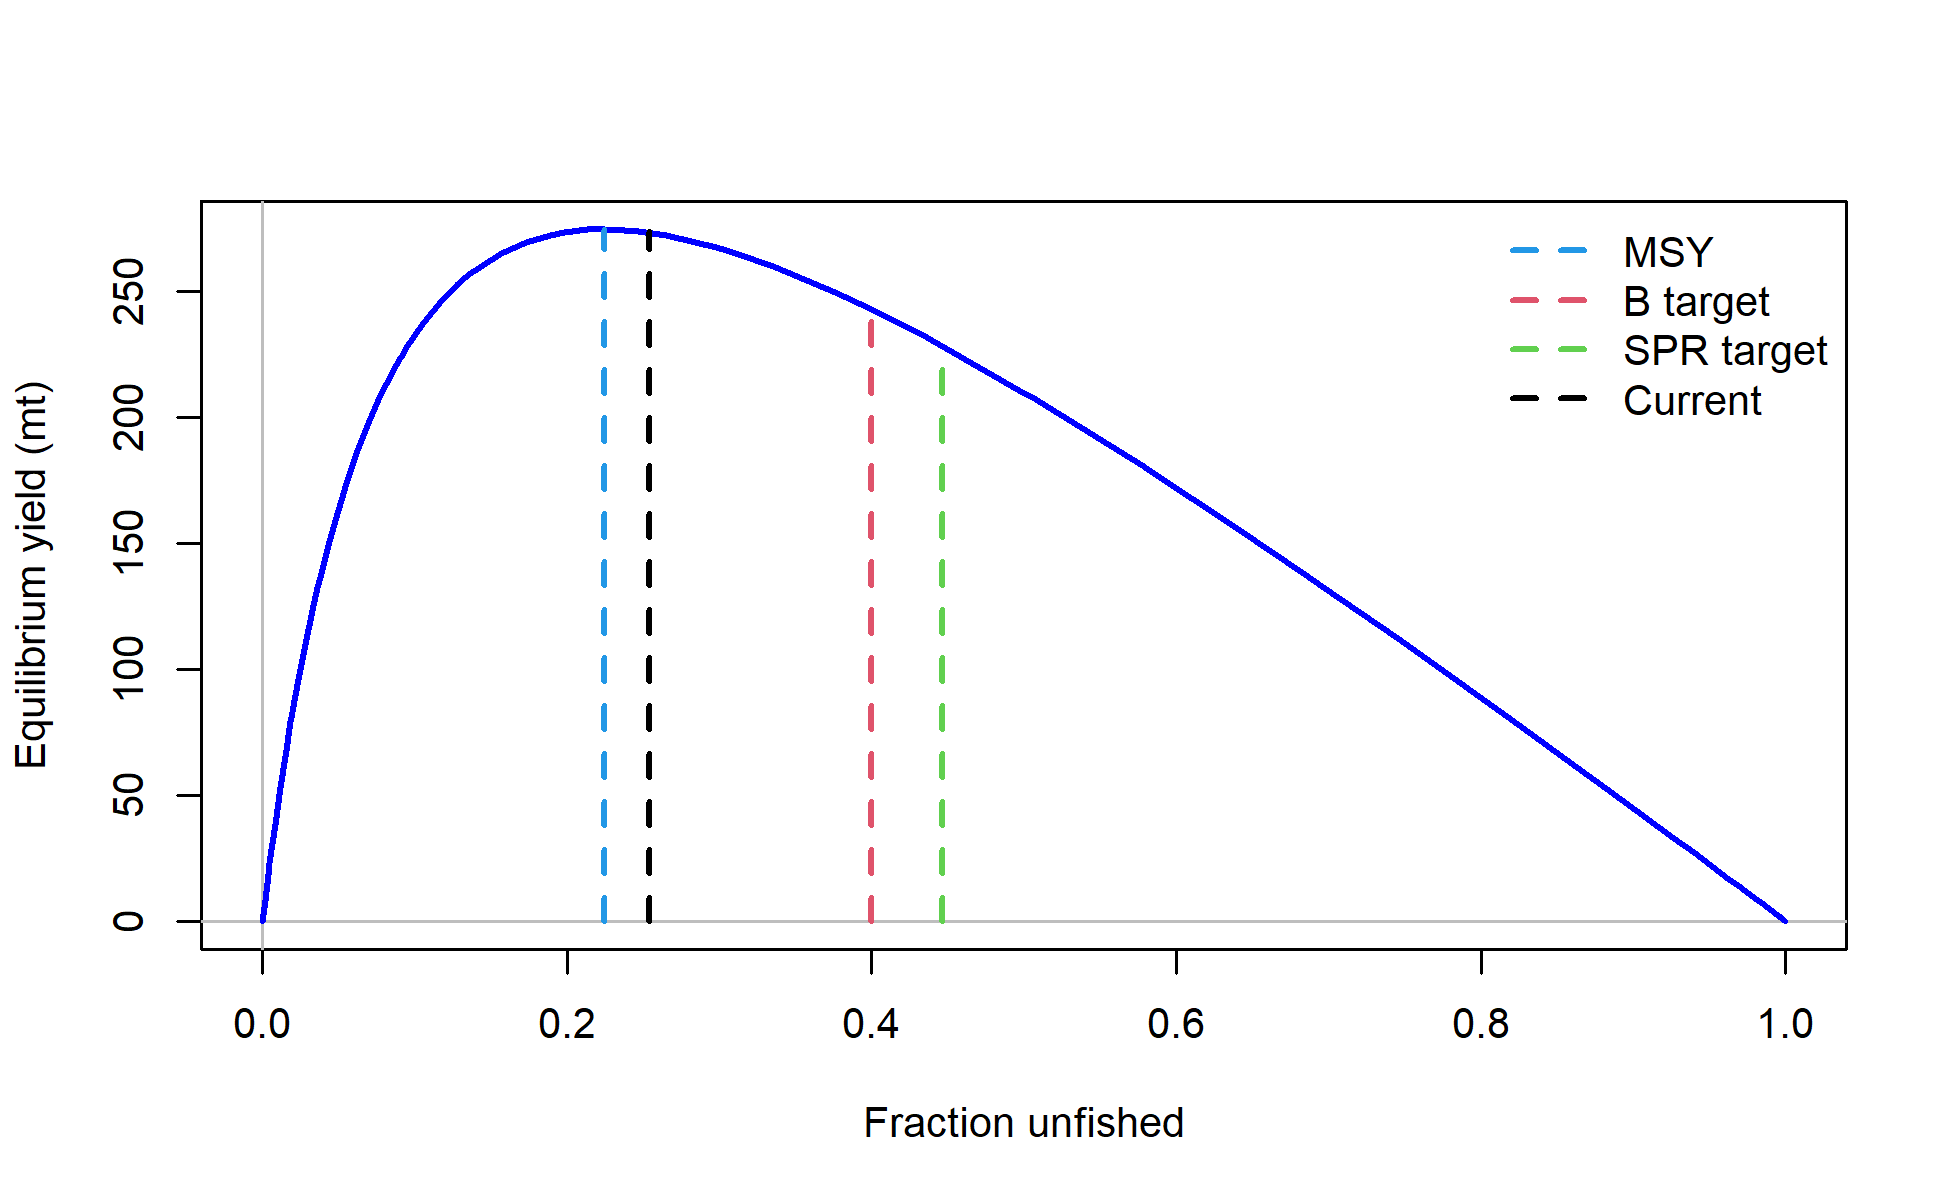
\includegraphics[width=1\textwidth,height=1\textheight]{C:/Users/Jason.Cope/Documents/Github/Sebastes_melanops_WA/Document/models/Reference model/plots/yield2_yield_curve_with_refpoints.png}
\caption{Equilibrium yield curve for the base case model. Values are based on (the time invariant) fishery selectivities and with steepness fixed at 0.72.\label{fig:es-yield}}
\end{figure}

\begingroup\fontsize{10}{12}\selectfont
\begingroup\fontsize{10}{12}\selectfont

\begin{longtable}[t]{r>{\centering\arraybackslash}p{2cm}>{\centering\arraybackslash}p{2cm}}
\caption{\label{tab:referenceES}Summary of reference points and management quantities, including estimates of the  95 percent intervals.}\\
\toprule
 & Estimate & Interval\\
\midrule
\endfirsthead
\caption[]{Summary of reference points and management quantities, including estimates of the  95 percent intervals. \textit{(continued)}}\\
\toprule
 & Estimate & Interval\\
\midrule
\endhead

\endfoot
\bottomrule
\endlastfoot
Unfished Spawning Output & 943.88 & 867.65-1020.10\\
Unfished Age 0+ Biomass (mt) & 8704.38 & 7999.16-9409.60\\
Unfished Recruitment (R0) & 1959.43 & 1801.19-2117.67\\
Spawning Output (2023) & 426.15 & 251.53-600.77\\
Fraction Unfished (2023) & 0.45 & 0.30-0.60\\
\underline{Reference Points Based on SB40\%} & \\
Proxy Spawning Output SB40\% & 377.55 & 347.06-408.04\\
SPR Resulting in SB40\% & 0.46 & 0.46-0.46\\
Exploitation Rate Resulting in SB40\% & 0.05 & 0.05-0.05\\
Yield with SPR Based On SB40\% (mt) & 293.52 & 269.82-317.22\\
\underline{Reference Points Based on SPR Proxy for MSY} &  & \\
Proxy Spawning Output (SPR50) & 421.11 & 387.11-455.12\\
SPR50 & 0.50 & -\\
Exploitation Rate Corresponding to SPR50 & 0.05 & 0.05-0.05\\
Yield with SPR50 at SB SPR (mt) & 275.88 & 253.60-298.17\\
\underline{Reference Points Based on Estimated MSY Values} &  & \\
Spawning Output at MSY (SB MSY) & 212.51 & 195.32-229.69\\
SPR MSY & 0.30 & 0.30-0.30\\
Exploitation Rate Corresponding to SPR MSY & 0.08 & 0.08-0.08\\
MSY (mt) & 332.18 & 305.38-358.98\\*
\end{longtable}
\endgroup{}
\endgroup{}


\clearpage

\hypertarget{management-performance}{%
\subsection*{Management performance}\label{management-performance}}
\addcontentsline{toc}{subsection}{Management performance}

Black Rockfish removals have generally been below the equivalent ABC-ACL over the recent decade, with the exception of 2017 and 2022 when removals were slightly higher (Table \ref{tab:manageES}). Exploitation on Black Rockfish increased starting around 1940 and reached a high in the late 1970s. Since that time, catch has mostly fluctuated between 300 and 500 mt per year, with some years exceeding 600 mt. Removals have averaged 483 mt over the past decade. The last ten years of Black Rockfish acceptable biological catch (ABC) and annual catch limit (ACL) (which are equivalent) has been set, by definition, below the overfishing limit (OFL) (Table \ref{tab:manageES}). Prior to 2017, management specifications were set for Black Rockfish in California and Oregon waters combined. The Black Rockfish OFL has not been exceeded by Oregon removals over the past decade.

\hypertarget{unresolved-problems-and-major-uncertainties}{%
\subsection*{Unresolved problems and major uncertainties}\label{unresolved-problems-and-major-uncertainties}}
\addcontentsline{toc}{subsection}{Unresolved problems and major uncertainties}

The biggest uncertainty and unresolved conflict is trying to reconcile the signal in the biological data (which suggests a lower population size and status) versus the acoustic and tag surveys (which suggest high stock sizes and status). This is the major issue the current assessment is confronting. Another acoustic-visual survey data point could help resolve how much uncertainty there is in the estimate. The lack of contrast in the biological data, despite large sample sizes, is another barrier to interpreting the current conditions, though given models using only biological data, the signal seems clear that the population could be at a lower stock status.

\hypertarget{scientific-uncertainty}{%
\subsection*{Scientific uncertainty}\label{scientific-uncertainty}}
\addcontentsline{toc}{subsection}{Scientific uncertainty}

The model-estimated uncertainty around the 2023 spawning biomass was \(\sigma\) = 0.2 and the uncertainty around the OFL was \(\sigma\) = 0.19. This is clearly an underestimate of overall uncertainty because of the necessity to fix some life history parameters such as natural mortality and steepness, as well as a lack of explicit incorporation of model structural uncertainty. The alternative states of nature used to bracket uncertainty in the decision table assist with encapsulating model structure uncertainty.

\hypertarget{harvest-projections-and-decision-table}{%
\subsection*{Harvest Projections and Decision Table}\label{harvest-projections-and-decision-table}}
\addcontentsline{toc}{subsection}{Harvest Projections and Decision Table}

The following text will be modified, as appropriate, after the STAR panel and SSC meeting.

The Black Rockfish assessment is being considered as a category 2 assessment with a \(P^*\) = 0.45, sigma = 0.72, and a time-varying buffer applied to the OFL. These multipliers are also combined with the rockfish MSY proxy of FSPR=50\% MSY and the 40-10 harvest control rule to calculate OFLs, ABCs and ACLs. A twelve year (2023-2034) projection of the reference model using these specifications along with input removals for 2023 and 2024 provided by the Groundfish Management Team is provided in Table \ref{tab:project_ES}.

Uncertainty in management quantities for the reference model was characterized by exploring various model specifications in a decision table. Initial explorations considered alternative specifications of natural mortality and population scale. Discussion with the STAR panel resulted in selecting a high state of nature based on a model that did not estimate recruitment deviations (i.e., recruitment was based solely on the stock-recruitment relationship). The low state of nature was based on a model that sought to estimate catchability for the acoustic-visual survey. High and low catch streams (rows) were determined by the forecasts, as described above, for each state of nature. Thus the low catch stream is based on the forecast from the low state of nature. The resultant decision table is provided in Table \ref{tab:es-dec-tab}.

\begingroup\fontsize{9}{11}\selectfont
\begingroup\fontsize{9}{11}\selectfont

\begin{longtable}[t]{c>{\centering\arraybackslash}p{1.38cm}>{\centering\arraybackslash}p{1.38cm}>{\centering\arraybackslash}p{1.38cm}>{\centering\arraybackslash}p{1.38cm}>{\centering\arraybackslash}p{1.38cm}>{\centering\arraybackslash}p{1.38cm}>{\centering\arraybackslash}p{1.38cm}}
\caption{\label{tab:project_ES}Projections of potential OFLs (mt), ABCs (mt), the buffer (ABC = buffer x OFL), estimated spawning biomass, and fraction unfished for Oregon portion of the vermilion stock. The North of 40°10'N OFL and ABC for 2021 and 2022 are included for comparison.}\\
\toprule
Year & OFL 40°10'N & ACL 40°10'N & Predicted OFL & ABC Catch & Buffer & Spawning Output & Fraction Unfished\\
\midrule
\endfirsthead
\caption[]{Projections of potential OFLs (mt), ABCs (mt), the buffer (ABC = buffer x OFL), estimated spawning biomass, and fraction unfished for Oregon portion of the vermilion stock. The North of 40°10'N OFL and ABC for 2021 and 2022 are included for comparison. \textit{(continued)}}\\
\toprule
Year & OFL 40°10'N & ACL 40°10'N & Predicted OFL & ABC Catch & Buffer & Spawning Output & Fraction Unfished\\
\midrule
\endhead

\endfoot
\bottomrule
\endlastfoot
2021	&	9.70	&	8.10	&	13.01	&	12.96	&	1.00	&	21.37	&	0.73\\
2022	&	9.70	&	8.10	&	13.35	&	12.96	&	1.00	&	21.53	&	0.73\\
2023	&	-	&	-	&	13.41	&	12.54	&	0.94	&	21.75	&	0.74\\
2024	&	-	&	-	&	13.29	&	12.36	&	0.93	&	21.85	&	0.75\\
2025	&	-	&	-	&	13.03	&	12.06	&	0.93	&	21.74	&	0.74\\
2026	&	-	&	-	&	12.72	&	11.73	&	0.92	&	21.46	&	0.73\\
2027	&	-	&	-	&	12.41	&	11.38	&	0.92	&	21.08	&	0.72\\
2028	&	-	&	-	&	12.10	&	11.05	&	0.91	&	20.65	&	0.71\\
2029	&	-	&	-	&	11.82	&	10.74	&	0.91	&	20.20	&	0.69\\
2030	&	-	&	-	&	11.56	&	10.45	&	0.90	&	19.75	&	0.68\\
2031	&	-	&	-	&	11.31	&	10.18	&	0.90	&	19.33	&	0.66\\
2032	&	-	&	-	&	11.08	&	9.94	&	0.90	&	18.92	&	0.65\\*
\end{longtable}
\endgroup{}
\endgroup{}


Further details about selecting the decision table states of nature will be added here after the STAR panel.

Further details summarizing the results presented in the decision table will be added here after the STAR panel.

\clearpage

\begingroup\fontsize{9}{11}\selectfont
\begingroup\fontsize{9}{11}\selectfont

\begin{longtable}[t]{l>{\raggedright\arraybackslash}p{0.08\linewidth}>{\raggedright\arraybackslash}p{0.08\linewidth}>{\raggedright\arraybackslash}p{0.1\linewidth}>{\raggedright\arraybackslash}p{0.09\linewidth}>{\raggedright\arraybackslash}p{0.1\linewidth}>{\raggedright\arraybackslash}p{0.09\linewidth}>{\raggedright\arraybackslash}p{0.1\linewidth}>{\raggedright\arraybackslash}p{0.09\linewidth}}
\caption{\label{tab:es-dec-tab}Decision table summary of 10 year projections beginning in 2023 for alternative states of nature based on an axis of uncertainty related to model structure relative to the reference model. Columns range over low (12.5 quantile), mid (reference model), and high states (87.5 quantile) of nature and rows range over different catch level assumptions. The first two years are fixed by the current harvest specifications.}\\
\toprule
\multicolumn{3}{c}{ } & \multicolumn{2}c{low $lnR_0$} & \multicolumn{2}c{Reference Model} & \multicolumn{2}c{High $lnR_0$} \\
\cmidrule(l{3pt}r{3pt}){4-5} \cmidrule(l{3pt}r{3pt}){6-7} \cmidrule(l{3pt}r{3pt}){8-9}
  & Year & Catch & Spawning Output & Fraction Unfished & Spawning Output & Fraction Unfished & Spawning Output & Fraction Unfished\\
\hline
&	2023	&	201	&	352	&	0.39	&	426	&	0.45	&	557	&	0.56\\	
&	2024	&	201	&	348	&	0.39	&	427	&	0.45	&	562	&	0.56\\	
&	2025	&	228	&	343	&	0.38	&	423	&	0.45	&	562	&	0.56\\	
&	2026	&	225	&	335	&	0.37	&	416	&	0.44	&	554	&	0.55\\	
&	2027	&	224	&	331	&	0.37	&	412	&	0.44	&	548	&	0.55\\	
P*=0.4	&	2028	&	224	&	331	&	0.37	&	411	&	0.43	&	543	&	0.54\\	
sigma=0.5	&	2029	&	225	&	33	&	0.37	&	412	&	0.44	&	541	&	0.54\\	
&	2030	&	226	&	340	&	0.38	&	416	&	0.44	&	540	&	0.54\\	
&	2031	&	227	&	346	&	0.39	&	421	&	0.45	&	541	&	0.54\\	
&	2032	&	228	&	354	&	0.39	&	427	&	0.45	&	543	&	0.54\\	
&	2033	&	228	&	361	&	0.40	&	433	&	0.46	&	546	&	0.54\\	
&	2034	&	226	&	368	&	0.41	&	439	&	0.48	&	548	&	0.55\\	
\hline																	
	&	2023	&	201	&	352	&	0.39	&	426	&	0.45	&	557	&	0.56\\	
	&	2024	&	201	&	348	&	0.39	&	427	&	0.45	&	562	&	0.56\\	
	&	2025	&	245	&	343	&	0.38	&	423	&	0.45	&	562	&	0.56\\	
	&	2026	&	241	&	333	&	0.37	&	414	&	0.44	&	552	&	0.55\\	
	&	2027	&	240	&	326	&	0.36	&	407	&	0.43	&	543	&	0.54\\	
P*=0.45	&	2028	&	241	&	325	&	0.36	&	404	&	0.43	&	537	&	0.54\\	
sigma=0.5	&	2029	&	242	&	326	&	0.36	&	404	&	0.43	&	532	&	0.53\\	
	&	2030	&	244	&	330	&	0.37	&	406	&	0.43	&	530	&	0.53\\	
	&	2031	&	245	&	335	&	0.37	&	410	&	0.43	&	529	&	0.53\\	
	&	2032	&	246	&	341	&	0.38	&	414	&	0.44	&	529	&	0.53\\	
	&	2033	&	247	&	347	&	0.39	&	418	&	0.44	&	530	&	0.53\\	
	&	2034	&	248	&	352	&	0.39	&	423	&	0.45	&	531	&	0.53\\	
\hline																	
	&	2023	&	201	&	352	&	0.39	&	426	&	0.45	&	557	&	0.56\\	
	&	2024	&	201	&	348	&	0.39	&	427	&	0.45	&	562	&	0.56\\	
	&	2025	&	279	&	343	&	0.38	&	423	&	0.45	&	562	&	0.56\\	
	&	2026	&	279	&	328	&	0.36	&	409	&	0.43	&	547	&	0.55\\	
Equilibrium	&	2027	&	279	&	317	&	0.35	&	398	&	0.42	&	533	&	0.53\\	
yield	from	&	2028	&	279	&	311	&	0.35	&	390	&	0.41	&	522	&	0.52\\
FMSY	proxy	&	2029	&	279	&	308	&	0.34	&	386	&	0.41	&	513	&	0.51\\
of	SPR=0.5	&	2030	&	279	&	309	&	0.34	&	384	&	0.41	&	507	&	0.50\\
	&	2031	&	279	&	311	&	0.35	&	384	&	0.41	&	502	&	0.50\\	
	&	2032	&	279	&	314	&	0.35	&	386	&	0.41	&	500	&	0.50\\	
	&	2033	&	279	&	317	&	0.35	&	388	&	0.41	&	498	&	0.50\\	
	&	2034	&	279	&	320	&	0.36	&	390	&	0.41	&	497	&	0.50\\*	
\hline
\end{longtable}
\endgroup{}
\endgroup{}


\clearpage

\hypertarget{research-and-data-needs}{%
\subsection*{Research and data needs}\label{research-and-data-needs}}
\addcontentsline{toc}{subsection}{Research and data needs}

Recommended avenues for research to help improve future Black Rockfish stock assessments:

\begin{enumerate}
\def\labelenumi{\arabic{enumi}.}
\tightlist
\item
  The availability of a comprehensive nearshore research survey for Black Rockfish (as well as for other nearshore rockfish species) was instrumental in providing the stock assessment with an estimate (and associated uncertainty) of population scale. Given this importance, continue the acoustic-visual fisheries independent coastwide survey to develop a time series. Evaluate survey improvements and analytical refinements as suggested in the SSC methodology review. Examine alternative spatial modeling approaches to better leverage the available information content toward reducing uncertainty in the absolute estimates of population size.
\item
  Improve understanding of broader ecosystem considerations within the context of Black Rockfish (and other nearshore species) management. Evaluate and develop linkages between Black Rockfish population dynamics and environmental, oceanographic, and climate variables. In particular, develop multi-scale models (e.g., species distribution models) that can evaluate spatial patterns (e.g., multi-use areas or closures to fishing) and climate impacts (e.g., growth or distribution shifts) for vulnerable nearshore species. Utilize the growing body of ecosystem information available for the California Current Large Marine Ecosystem, as exemplified in the PFMC IEA report.
\item
  Continue work on the investigation into the movement, behavior or mortality of older (\textgreater{} age 10) females to further reconcile their absence in fisheries data. In particular, conduct genetics studies on fish observed off of the continental shelf (middle of the gyre and at sea mounts) to determine their association with the nearshore stocks.
\item
  Continue to build evidence for appropriate natural mortality values for females and males. This will help resolve the extent to which dome-shaped age-based selectivity may be occurring for each.
\item
  Design and conduct research studies to better understand the tradeoffs revealed in this assessment between Black Rockfish biology and population scale that seem be at odds. If discrepancies can not be uncovered, evaluate management procedures that are as robust as can be to this tradeoff.
\item
  Conduct early life history studies that provide a better understanding of the ecology and habitats of Black Rockfish from settlement to age-1.
\end{enumerate}

\vspace{500cm}

\pagebreak
\setlength{\parskip}{5mm plus1mm minus1mm}
\pagenumbering{arabic}
\setcounter{page}{1}
\renewcommand{\thefigure}{\arabic{figure}}
\renewcommand{\thetable}{\arabic{table}}
\setcounter{table}{0}
\setcounter{figure}{0}

\hypertarget{introduction}{%
\section{Introduction}\label{introduction}}

\hypertarget{basic-information}{%
\subsection{Basic Information}\label{basic-information}}

Black Rockfish (\emph{Sebastes melanops}) are an important component of the recreational fisheries in the nearshore waters off central and northern California, Oregon, and Washington, as well as the non-trawl commercial fisheries in California and Oregon. They range as far north as Amchitka and Kodiak islands in Alaska and are considered uncommon south of central California (Milton S. Love, Yoklavich, and Thorsteinson 2002).

A first assessment of Black Rockfish off considered the population off Oregon and California (S. Ralston and Dick 2003) and reviewed the evidence supporting genetic stock structure for Black Rockfish and other rockfish off the U.S. West Coast and concluded that the Oregon and California populations of Black Rockfish are probably not genetically heterogeneous. That assessment treated the Black Rockfish off California and Oregon as a unit stock. Previous assessments of Black Rockfish off Washington (F. R. Wallace, Hoffman, and Tagart 1999; Y. W. Wallace F. R. aand Cheng and Tsou 2007) describe a study of coastal Black Rockfish genetic structure using 10 sampled sites collected from northern California to southern British Columbia t 1995-97. Results of that study support the notion of separate genetic stocks north and south of Cape Falcon. However, a later study (Baker 1999) of Black Rockfish collected from eight sites along the northern Oregon coast concluded that Black Rockfish from north and south of Cape Falcon were genetically very similar.

Although a stock boundary line at the Columbia River seems reasonable for Black Rockfish, both because it is a state fishery management boundary and because the Columbia River plume is likely to be a natural barrier to the north-south exchange of Black Rockfish adults and larvae, the 2007 assessment of Black Rockfish off Oregon and California (Sampson 2007) differed slightly from Ralston and Dick (2003) in placing the northern boundary at Cape Falcon rather than at the Columbia River. The boundary was changed to avoid overlap with the separate northern assessment (Y. W. Wallace F. R. aand Cheng and Tsou 2007) and to simplify the process of assembling historical commercial landings data, which are largely available in terms of Pacific Marine Fisheries Commission (PMFC) statistical areas. The northern boundary of PMFC Area 2C is at Cape Falcon (Figure 1). Given the spatial resolution of the historical commercial fishery data, it is very problematic to estimate the catch of Black Rockfish taken north of Cape Falcon but south of the Columbia River.

During a preliminary workshop in April 2015 (Council 2015), to discuss approaches for assessing Black Rockfish, China rockfish (\emph{S. nebulosus}), and kelp greenling (\emph{Hexagrammos decagrammus}), it was agreed that the assessments for these nearshore species should at a minimum be spatially stratified with boundaries at the CA/OR border (42\textdegree00' N latitude) and the OR/WA border (46\textdegree16' N latitude). Such a spatial stratification would be consistent with two ideas: (a) these nearshore species do not exhibit much adult movement and (b) exploitation and management histories have varied significantly among the three states. Together these features would likely create appreciable state-to-state differences in age composition for each of the three species. Stock assessment teams were advised that they could use geographic strata that were finer than the state level if there were data to support such an approach (Figure 1).

At the same nearshore stock assessment workshop, it was agreed that recreational catch histories for the stocks of Black Rockfish should be assembled on the basis of port of landing rather than location of fish capture, even though fishing vessels landing their catches into a port in one state might have captured fish in waters off a neighboring state.

Accounting for location of capture is very problematic for recreationally caught fish and for commercial catches taken with non-trawl types of gear (e.g., hook-and-line), for which there are no or very limited logbooks that report fishing location. For these regional assessments the commercially caught Black Rockfish were apportioned to assessment region based on the port of landing, with the exception of trawl caught fish landed into Astoria, OR. Most of these fish were assumed to have been caught off Washington and most of the trawl landings into Astoria were therefore included with the catch history for the Washington assessment region. Details are provided below in Section 2.1.1.1 The PacFIN Era (1981 to 2014).

\hypertarget{life-history}{%
\subsection{Life History}\label{life-history}}

Adults tend to occur in schools over rocky structure at depths less than 40 fathoms, and sometimes feed actively on or near the surface. They feed on a wide variety of prey including zooplankton, krill, mysids, sand lance, and juvenile rockfish, and are subject to predation by lingcod and marine mammals (Milton S. Love, Yoklavich, and Thorsteinson 2002).

Although tagging studies have documented some individuals moving long distances (several hundreds of miles), the vast majority of recaptured individuals were found close to the areas of initial capture and tagging (Culver 1987; Ayres 1988; Wallace F. et al. 2010; Starr and Green 2007). Results from a 2004-05 study off Newport, OR of 42 Black Rockfish implanted with acoustic tags indicated that all but seven fish remained within range of a 3 x 5 km array of acoustic receivers during one full year of monitoring and had relatively small home ranges that did not vary seasonally (S. J. Parker et al. 1995). Green and Starr (2011) report similar findings from a study in Carmel Bay, CA of 23 acoustically tagged Black Rockfish. The extensive Washington state tagging study also supported low movements for most individuals, with some exceptional movements recorded (Wallace F. et al. 2010).

Like all members of the genus Sebastes, Black Rockfish have internal fertilization and bear live young approximately two months after insemination. Black Rockfish are quite fecund, with a six-year-old female annually producing about 300,000 embryos and a 16-year-old producing about 950,000 embryos (S. J. Bobko and Berkeley 2004). Recent studies have demonstrated that the relative number and quality of larvae increase with age in female Black Rockfish (S. A. Berkeley, Chaoman, and Sogard 2004; Hixon, Johnson, and Sogard 2014a). Parturition of larvae occurs during winter (Echeverria 1987) and larvae and small juveniles are pelagic for several months to a year (Boehlert and Yoklavich 1983). Settlement occurs in estuaries, tide-pools, and in the nearshore at depths less than 20 m (Stein and Hassler 1989).

Black Rockfish begin recruiting to nearshore fisheries at 3-4 years of age, corresponding to a fork length of about 25-30 cm, and 50\% of females attain maturity at about 6-8 years, corresponding to a fork length of about 38-42 cm. Adult female Black Rockfish grow 3-5 cm larger than males, with a few females attaining fork lengths greater than 55 cm.

\hypertarget{ecosystem-considerations-1}{%
\subsection{Ecosystem Considerations}\label{ecosystem-considerations-1}}

No formal ecosystem considerations have been made given the lack of data for such an undertaking. Differences in growth though time have been considered in the model specification in the Washington model. Though the mechanism is not specified, this could certainly be due to process error driven by environmental conditions.

\hypertarget{historical-and-current-fishery-information}{%
\subsection{Historical and Current Fishery Information}\label{historical-and-current-fishery-information}}

Black Rockfish are harvested by a wide variety of fishing methods including trawling, trolling, and hook-and-line fishing with jigs and long-lines. Although Black Rockfish have never been a dominant component of any commercial fisheries, they are important as incidental catch in the troll fishery for salmon and the troll and jig fisheries for groundfish. With the decline of salmon fishing opportunities in the late 1970s and early 1980s Black Rockfish became a vital target of marine recreational fisheries in Oregon and Washington, especially during periods of restricted or slack fishing for salmon, halibut, and tuna.

Black Rockfish are also an important component of the recreational fisheries in northern California but are of less significance south of Cape Mendocino due to their reduced prevalence compared to other species. Since 1990 annual recreational harvests of Black Rockfish have averaged 229.6 tons off California, 304.4 tons off Oregon, and 272.5 tons off Washington. Commercial annual harvests by non-trawl gear types during the same period averaged 44.6 tons in California, 62.0 tons in Oregon, and 14.7 tons in Washington. Harvests by trawl on average during this period have been less than 19.3 tons annually for all three states combined.

Removal histories have been a significant axis of uncertainty in the past assessments of Black Rockfish. Because of concerns about the effects of initial equilibrium assumptions on the level of depletion estimated in the preliminary base model, the 2003 Stock Assessment Review (STAR) panel worked with the Stock Assessment Team (STAT) to develop a catch history that avoided the need to assume historical catch and equilibrium conditions in the first year of the assessment. The assumed catch reconstruction began in 1946, ramping up from zero in 1945 and all prior years. In hindsight, this may not have been a good assumption, as indicated by the following text from (Cleaver 1965) that describes catches of rockfish from 1941 to 1949 in Oregon.

``The rockfish are caught by otter trawl and long-line gear. The principal species caught by the otter trawl are the Black Rockfish (\emph{Sebastodes melanops}); green or yellowtail rockfish (\emph{S. flavidus}); red or orange rockfish (\emph{S. pinniger}); and rosefish (\emph{S. alutus}). The landings of rockfish (all species) rose rapidly during the war from 1,301,400 pounds in 1941 to a peak of over 17,000,000 in 1945. Subsequently the landings fell rapidly because of decreased demand and leveled off at about 4,000,000 per year in 1949.

Cleaver (1965) also states, in an introductory section on Bottom Fisheries, that the ``otter trawl fishery accounts for at least 95 percent by weight of the bottom fish landings.''

That Black Rockfish is one of only four species that Cleaver (1965) identifies as composing the large landings of rockfish in Oregon (most of which was actually taken off of Washington waters) during WWII suggests that Black Rockfish were not a trivial fraction of the large catches taken during the 1940s. One might also suppose that the otter trawl fishery took a large portion of the landings of Black Rockfish. Cleaver's statements are certainly at odds with the catch reconstruction developed in the previous assessments.

It seems that Black Rockfish were also landed in appreciable quantities in California during the 1940s. Black Rockfish was identified by scientific name as one of the ``half-dozen of the larger and more abundant species {[}that{]} make up over half of the annual California commercial poundage landed'' (Anon. 1949).

A major task for the 2007 assessments of Black Rockfish in was developing a plausible reconstruction of historical landings of Black Rockfish and exploring the consequences of those landings. For the current set of assessments catch histories from the past assessments have been reconsidered. Formal catch reconstructions have been conducted in California (Stephen Ralston et al. 2010) and Oregon (Karnowski, Gertseva, and Stephens 2014), but even those relatively newer attempts were reconsidered in light of contributions from state agencies. For this assessment, Washington provided a first step in an approach to provide a reconstructed historical catch time series for a stock, something needed for all species in the state's waters.

\hypertarget{summary-of-management-history-and-performance}{%
\subsection{Summary of Management History and Performance}\label{summary-of-management-history-and-performance}}

Prior to 2000 the Pacific Fishery Management Council (PFMC or Council) managed the fishery for Black Rockfish as part of the Sebastes complex, with no separate Acceptable Biological Catch (ABC) or Optimum Yield (OY) for Black Rockfish. In 2000 the Council established an ABC of 1,200 mt for Black Rockfish caught north of Cape Mendocino (in the Eureka, Columbia, and Vancouver INPFC statistical areas), but left Black Rockfish south of Cape Mendocino as part of the ``other rockfish'' category. For 2001 through 2003 the ABC for Black Rockfish caught north of Cape Mendocino was 1,115 mt annually, and Black Rockfish south of Cape Mendocino remained part of the ``other rockfish'' category and without a separate ABC or OY.

Regulation of the Black Rockfish fisheries by the PFMC prior to 2004 was accomplished primarily by trip limits for commercial fisheries and bag limit restrictions for recreational fisheries, with different limits applying in different geographic regions (see Table 1 in S. Ralston and Dick (2003)). Some other important regulations include the following.

\begin{itemize}
\tightlist
\item
  1953: California prohibited trawling within three miles of shore.
\item
  1995: The commercial hook-and-line fishing in Washington state waters (0-3 miles) was closed to preserve recreational fishing opportunities and avoid localized depletion; the closure was extended to trawlers in 1999. Oregon established Black Rockfish management areas with reduced daily commercial fishery trip limits in area near ports with large recreational fisheries.
\item
  2000: Black Rockfish began to be managed by the Council as a minor nearshore species. Commercial trip limits were significantly reduced, with specific restrictions applying to Black Rockfish. California instituted seasonal closures for commercial and recreational fisheries inside 20 fathoms, reduced the bag limit for rockfish from 15 to 10 fish, and limited recreational gear to one line with three hooks.
\item
  2002: California adopted a Nearshore Fishery Management Plan and began more active management of nearshore fisheries including the use of seasonal, regional, and depth-specific closures. Oregon adopted an Interim Nearshore Fishery Management Plan in anticipation of increased pressure on nearshore stocks due to reduced fishing opportunities for groundfish in federal waters. Regulations included fishing-sector specific caps on retained harvests, set approximately at the levels attained in 2000.
\item
  2003: The Council established Rockfish Conservation Areas (RCAs) to control catches of overfished rockfish species, and large portions of the shelf were closed to fishing. Differential trip limits were applied north and south of a management boundary at 40\textdegree10' N. latitude for nearshore Sebastes species. Nearshore permittees in California became subject to depth restrictions consistent with the shoreward non-trawl RCA boundary. In California the commercial and recreational fisheries for rockfish were closed early.
\item
  In 2004 and 2005: the sport fishery in Oregon closed in September 2004 due to early attainment of the state's limit for sport-caught Black Rockfish. This was the first time that the sport rockfish fishery in Oregon had not been open all year. In 2005 it closed early again.
\item
  In 2008 the groundfish trawl fishery was closed in Washington from the seaward RCA boundary to the shore north of 48\textdegree10' N. latitude to address increased encounters with yelloweye rockfish and canary rockfish.
\end{itemize}

In recent years California, Oregon and Washington regulations for the marine sport fisheries, which has been the major source of mortality on Black Rockfish, have become quite complicated and variable through time. Tools for regulating the sport fishery include closed areas, depth restrictions, seasonal closures, and bag limits.

California had no recreational bag limit for rockfish until 1990 when a 15 fish per day per angler limit was implemented. In 2000 the limit was reduced to 10 fish per day for each angler's combined bag of rockfish, cabezon and greenling. The fishing season was year-round prior to 2000 and since then has been variable by state management area. There were no gear restrictions prior to 2000. In 2000 anglers were limited to fishing one line with three hooks. Since 2001 they have been restricted to one line with two hooks. There is no minimum size limit for Black Rockfish.

Oregon had no recreational bag limits for marine fishes until 1976 when the state established a 25-fish limit. In 1978 the state established a daily limit of 15 fish for each angler's combined bag of rockfish, cabezon and greenling, which stayed in effect until 1994 when the state established a 10-fish-per-angler daily bag limit specifically for Black Rockfish. Following the early closure of the fishing season for Black Rockfish in 2004, the daily bag limit for Black Rockfish was dropped to 5 fish at the start of 2005 but was increased in-season to 6 fish. The per-angler daily bag limit was 6 fish during 2006 and 2007, 5 fish at the start of 2008 and increased in-season to 6 fish, 6 fish at the start of 2009 and increased in-season to 7 fish where it has remained since.

The goal of Oregon's sport fishery management is to maintain year-round fishing opportunities. In-season adjustments to regulations can be made more restrictive or less restrictive, depending on circumstances and the prospects for early attainment of harvest caps. Seasonal depth restrictions (e.g., inside 30 fathoms April 1 to September 30) are one tool used regularly in recent years to control the fishery, driven largely by the need to avoid bycatch of the primary rebuilding species, canary rockfish and yelloweye rockfish.

Washington had a recreational daily bag limit for rockfish (all species) of 15 fish per day from 1961 to 1991, 12 fish per day from 1992 to 1994, and 10 fish per day from 1995 to 2015. The bag limit for blue rockfish plus Black Rockfish in Marine Area 4B (Neah Bay) has been 6 fish per day since 2010. Fishing seasons for groundfish species are structured to provide year-round fishing opportunities, if possible. Depth restrictions vary by state management area, being more restrictive in the north compared to the south due to higher encounter rates with overfished yelloweye rockfish and canary rockfish. There is no minimum size limit for Black Rockfish.

In 2004 the coastwide ABC established for Black Rockfish was based on the projected yields derived from separate northern {[}wallace\_status\_1999{]} and southern {[}ralston\_status\_2003{]} stock assessments (Table 1). The northern assessment covered the Washington coast and the northernmost portion of Oregon, from Cape Falcon to the WA/OR border at the Columbia River. The southern assessment covered the entire Oregon coast and the California coastline north of Point Arena.

To account for the spatial overlap of the two assessment areas, 12\% of the projected yield from the northern assessment was transferred to the southern region when deriving the coastwide ABC and OY values of 1,315 mt for 2004. State-by-state harvest guidelines were established: 326 mt for California, 450 mt for Oregon, and 540 mt for Washington. A similar approach was taken in 2005 and 2006 and the OY for the area south of the Columbia River was apportioned to harvest guidelines for California and Oregon based on a 42:58 split. The basis for this apportionment is unclear was to support separate harvest guidelines for each state. The catches were apportioned by the average catch share by state in the 1985-2002 period (Council 2004).

In all years when there has been an OY specified for Black Rockfish the estimated catch has been less than the OY, except for 2003 when the estimated coastwide catch exceeded the ABC for north of Cape Mendocino. In 2003 the estimated coastwide catch exceeded the OY by 183 mt for the region north of Cape Mendocino, but 290 mt of this coastwide catch was recreational harvest taken south of Cape Mendocino.

\hypertarget{canadian-and-alaska-fisheries}{%
\subsection{Canadian and Alaska fisheries}\label{canadian-and-alaska-fisheries}}

Black Rockfish is a ``Non-Quota'' species in the Department of Fisheries and Oceans Management Plan, and is not formally assessed in nearshore Canada waters (Fisheries and Canada 2014).

Add Alaska assessment text here.

\hypertarget{data-and-model-inputs}{%
\section{Data and Model Inputs}\label{data-and-model-inputs}}

A description of each data source is provided below (Figure \ref{fig:data-plot}).

\hypertarget{fishery-dependent-data}{%
\subsection{Fishery-Dependent Data}\label{fishery-dependent-data}}

\hypertarget{commercial}{%
\subsubsection{Commercial}\label{commercial}}

\hypertarget{landings}{%
\paragraph{Landings}\label{landings}}

The systems along the U.S. West Coast for monitoring commercial fishery landings in the past did not keep track of the landings of individual rockfish species, largely because many rockfish species have similar market characteristics and therefore were landed as an unsorted mix of species. Black rockfish in particular, which are a nearshore species and much less abundant than many of the offshore rockfish species, were generally landed in mixed-species categories and not required to sort into its own market category until 2006. As a consequence, the historical records do not provide a detailed accounting of the landings of black rockfish. The basic approach taken to develop the landings series in this assessment (as in past assessments) was to apply values for the proportion of black rockfish sampled in mixed-rockfish landings. Data on the proportions of black rockfish are sparse, with the consequence that the landings reconstructions are highly uncertain.

Commercial fishery landings of black rockfish in Washington are compiled from a variety of sources including PacFIN, agency reports, historical fish ticket information and communication with agency personnel (Table 48). Since 1935, commercial fishing vessels have been required to submit a fish receiving ticket (``fish ticket'') for each landing. Rockfish landings from domestic fishers are usually reported in mixed-species market categories, and are routinely sampled for species composition by port samplers. The information required on the ticket and sampling methods have changed through time. Due to these changes, we separated the data into three time periods 1935-1969, 1970-1980, and 1981-present based on the level of detail available in the data for compiling landing history in Washington for this assessment. Comparisons of the commercial catch in each fishery for the current and previous assessments (Figure X).

\hypertarget{years-1935-to-1969}{%
\subparagraph{Years 1935 to 1969}\label{years-1935-to-1969}}

Although the original paper fish tickets are no longer available for this period, WDFW recently digitized the daily aggregated data from printed reports, to assist in reconstructing the commercial groundfish fishery landings history for Washington. These daily aggregated data reports contain summaries of daily catches for port-groups by gear and area fished. The data are available for 1935 and for 1949-1969, and were used as the basis for the black rockfish catch reconstruction for this time period.

During this period, mixed-species, nominal market categories were typically used for reporting of the aggregated data. Market categories such as ``red rockfish'', ``black rockfish'' (BLK1), and ``unidentified rockfish'' (URCK) are typical on fish tickets during this time, lumping all red colored fish and black colored fish into these categories for reporting. For bottom trawl gears, the BLK1 market category consisted of mostly yellowtail rockfish and silvergrey rockfish (Greg Lippert, pers. comm.). To split the black rockfish landings out of the BLK1 market category, we assumed 10\% of the BLK1 landings were S. melanops (BLCK). We further assumed that no other nominal market categories in the trawl fishery contained S. melanops (see table below).

For the commercial jig and troll fisheries, rockfish were landed in the unidentified rockfish (URCK) market category. No species composition samples are available during this time, so we assumed 85\% of URCK landings were S. melanops, which matches the species composition data from the 1985-1989 commercial jig fishery. These estimates were also supported by interviews with port samplers active during portions of this period. The rockfish caught by troll gears composed of mostly yellowtail and black rockfishes. Wright (1967) reported rockfish species composition of the troll landings by port. We assumed 80\% of URCK caught off central Washington were BLCK and 20\% for northern Washington landings.

\hypertarget{years-1970-to-1980}{%
\subparagraph{Years 1970 to 1980}\label{years-1970-to-1980}}

Original fish ticket data were used for commercial catch estimate during this period. Fishing areas were better defined and reported during this period; there were no longer interstate areas due to the introduction of current management areas, with a boundary line at the OR/WA state border. However, issues with URCK market category remained. Species composition sampling of URCK were conducted for trawl and jig fisheries but not for salmon troll and the ``other gears'' gear types.

To estimate the trawl landings of black rockfish in the category URCK, we applied the current WDFW species composition algorithm by gear, port, and quarter. If no species composition samples were taken during a quarter, we first borrowed annual composition data for the gear/port group. If those data were not available, a coastwide annual composition for the particular gear type was applied. There was no borrowing of composition information across gear groups or years.

The commercial jig fleet operates in nearshore waters and black rockfish is the dominant component of the URCK landing for this gear type. Species composition sampling was not conducted during the 1970-1980 time period. Based on the samples collected in the 1980s, we assumed that black rockfish made up 80\% of the total rockfish landed by the jig fleet. For the troll fishery, the same proportions as for the pre-1970 time period were applied.

Rockfish (URCK) were also landed in small amounts by other commercial fleets, such as fixed gears and salmon troll. The fleets in the 70s and 80s predominantly targeted sablefish and halibut in waters too deep for black rockfish. Port samplers did not recall observing any black rockfish in the fixed gear landings (James Beam and Greg Lippert, pers. comm.). Therefore, we assumed fixed gear landings were negligible. For URCK landed by the salmon troll fleet, the majority of troll landings was yellowtail rockfish with smaller numbers of widow, canary, and black rockfish (Wendy Beeghley and James Beam, pers. comm.). We assumed that 10\% of the troll rockfish landings were black rockfish for 1970-1980.

\hypertarget{years-1981-to-the-present-the-pacfin-era}{%
\subparagraph{Years 1981 to the Present (the PacFIN era)}\label{years-1981-to-the-present-the-pacfin-era}}

Commercial landings data for the modern era (1981 to present) are taken from the Pacific Fishery Information system (PacFIN), which is a central repository for U.S. West Coast groundfish landings and auxiliary information collected by the three state fishery agencies and other agencies. A description of basic state data collection systems and overview of PacFIN is provided in Sampson and Crone (1997). Updated dockside sampling protocols and data processing procedures for Washington are described in Tsou et al. (2015) and Tsou and Weyland (2015). Rockfish landings from this period are pulled from the PacFIN comprehensive catch table. Landings in this table are the products of nominal landings, as well as area and species compositions. For the remaining URCK in this table, we applied a coastwide annual composition for each gear, as described above. After this step, there are still small amounts of URCK for trawl and setline gears. These landings are not included in this assessment.

For the jig-gear fishery, dockside sampling was conducted by the WDFW Ocean Sampling Program (OSP) during 1985-1991. These species composition data are not available in PacFIN. For landings during 1985-1991 the URCK species compositions were stratified by year and port. For other years, species compositions were stratified by port only. For jig-caught fish landed into Seattle annual species compositions from Neah Bay were applied (Table 49) because there was no port sampling in Seattle. The URCK market category was used until 2000, after which it was replaced by the Slope, Shelf, and Nearshore rockfish market categories. The commercial nearshore fishery was closed in 1999, so starting in 2000 there are negligible black rockfish landings in any market categories. In 2005 mandatory sorting was established for black rockfish, so all black rockfish landed should be recorded on fish tickets in the BLK1 category.

To assign URCK commercial salmon troll landings, we used the same reasoning assumption as applied to earlier periods (see 1970-1980) to assign 10\% of the URCK landed in the salmon troll fishery to black rockfish. After a complete nearshore closure in 1999, black rockfish landings have been negligible.

It has been and continues to be a common practice for Oregon fleets to fish off Washington coast and land the catches at Oregon ports. Although the separate geographic assessments by state region would ideally have strict geographic separation of landed catch to the location of capture, this is not possible to accomplish because information on the fishing location is generally unavailable. Until recently logbooks that report area of capture were only available for landings by the groundfish trawl fleet. Oregon has required a logbook for commercial vessels participating in its nearshore fishery since 2004.

Staff from the Oregon Department of Fish and Wildlife (ODFW) used species composition samples collected during 1976 to 1993 to conduct an analysis of the spatial distribution of black rockfish landed at Astoria, OR. Astoria is the northernmost port in Oregon and is located near the mouth of the Columbia River, which forms the boundary between Oregon and Washington. The portion of aggregated rockfish landed pounds that were taken north of the Columbia River (i.e., from waters off Washington) was 98.6\%. This percentage was applied to all historical trawl landings of rockfish at Oregon's Columbia River District ports prior to 1976. It was assumed 14.1\% of the aggregated rockfish being Black in the 2015 assessment (Cope et at. 2016). This percentage is much higher than the values used for Washington catch reconstruction. Therefore, we recalculated the portion by using Washington historical species composition data not available in PacFIN for pre-1981 and data available in PacFIN for 1981 to 1986. The revised proportions of black rockfish in the aggregated rockfish landings are 3\% and 4\% for pre-1981 and 1981-1986, respectively. Non-trawl landings into Astoria were assumed to have been caught from Oregon waters, same assumption as used in 2015 assessment.

Starting in 1994 black rockfish landed into Oregon were legally required to be sorted and sold in a separate black rockfish market category and were also reported as separate retained catches in the mandatory trawl logbooks. Based on the retained catches reported in the logbooks, the estimated proportion of the trawl-caught black rockfish that were caught from off Washington and landed into Astoria ranged from 65 to 100 percent. These black rockfish are accounted for in the Washington regional assessment (Table X).

The Washington Department of Fish and Wildlife (WDFW) provided commercial fishery landings based on fish ticket records of black rockfish harvested off Oregon by vessels landing at ports in Washington. Landings were less than 1 mt per year for the period 1971 to 2014; therefore, all landings to Washington ports were assumed to occur in waters off Washington in this assessment.

\hypertarget{foreign-fishery-catches-of-black-rockfish}{%
\paragraph{Foreign Fishery Catches of Black Rockfish}\label{foreign-fishery-catches-of-black-rockfish}}

Rogers (2003) developed catch reconstructions for removals by foreign trawlers operating off the U.S. West Coast during the late 1960s to mid-1970s. Although this study reports that Japanese vessels operating in the Columbia and Eureka statistical areas (Oregon and northern California) caught substantial amounts of black rockfish, with cumulative catches of more than 500 mt over 10 years, it seems very unlikely that foreign vessels could have operated sufficiently close to shore to catch appreciable amounts of black rockfish. This assessment does not include Rogers' estimates of foreign fleet removals of black rockfish.

\hypertarget{recreational-removals}{%
\subsubsection{Recreational Removals}\label{recreational-removals}}

Comparisons of the catch in each recreational fishery for the current and previous assessments are in Figure X.

The Washington recreational catch history of black rockfish was reconstructed using several direct and indirect records of black rockfish catch (Table X). All primary sources report catch in numbers of fish. As sources have been modified and re-evaluated, a completely new catch reconstruction for Washington was developed for 2015 assessment. This catch history was updated to include 2015-2022 estimates in this assessment.

\hypertarget{estimated-discards}{%
\subsubsection{Estimated Discards}\label{estimated-discards}}

In the previous assessment, commercial discards were not accounted for due to the information provided by the West Coast Groundfish Observer Program (WCGOP) at that time, showing about a 1\% discard rate in their survey. We evaluated the WCGOP estimates of black rockfish discards from 2002-2013, which showed a total of 32.2 mt in estimated discards and total landings of 2042.5 mt coastwide, resulting in a rough discard rate estimate of 1.58\%. This amount of discards was included in the CA HKL non-live fishery landings, going back to 1916, and in the OR HKL non-live fishery landings to 1892. Given the minimal amount of discards, no further depth-dependent mortality estimates were evaluated for Oregon and California and this discard rate was added to the total commercial removals. Parker et al (2006) concluded that semi-pelagic, vertically mobile species, such as black rockfish, show less barotrauma; hence these estimates could be slightly overestimated.

Washington recreational discard estimates were not available until 2002. Numbers of discarded-by-depth black rockfish were estimated using the same catch expansion algorithm for landed catch. Surface release mortalities adopted by the Groundfish Management Team (GMT) in their death-by-depth matrix (11\%, 20\%, 29\%, and 63\%) were then applied to the number of release black rockfish for each of 4 release depth bins (0-10 fm, 11-20 fm, 21-30 fm, and \textgreater30fm), respectively. Total dead released black rockfish were then summed across each depth bin. The average weights of discards were assumed to be the same as the average weights of landed and multiplied by the number of released dead to get total dead in metric tons. For pre-2002 release, proportions of releases based on a ratio estimator using 2003-2007 data were applied. For the split between charter and private vessels, the same algorithm used for splitting retained catch was applied. The overall average discard rate in the recreational fisheries was 1.37\%. There was no information on Washington commercial discards, so the rate of 1.37\% (same as the historical recreational discards) was also applied to the entire commercial time series. This low rate was similar to discard rates estimated in the other states.

\hypertarget{size-and-age-composition-data}{%
\subsection{Size and Age Composition Data}\label{size-and-age-composition-data}}

Fish length measurements, primarily from the recreational fishery, are one of the major sources of data for this assessment.

\hypertarget{length-and-age-sample-sizes}{%
\subsubsection{Length and Age Sample Sizes}\label{length-and-age-sample-sizes}}

The level of commercial fishery sampling for black rockfish has been erratic, with almost no samples taken in Washington until the early 1990s (Figure X).

\hypertarget{multinomial-sample-sizes}{%
\paragraph{Multinomial Sample Sizes}\label{multinomial-sample-sizes}}

Initial input values for the multinomial samples sizes determine the relative weights applied in fitting the annual composition data within the set of observations for each fishery. The initial input values in this assessment were based on the following equation developed by I. Stewart and S. Miller (NWFSC), and presented at the 2006 Stock Assessment Data and Modeling workshop. Neff = Ntrips + 0.138 * Nfish if Nfish/Ntrips \textless{} 44 Neff = 7.06 * Ntrips if Nfish/Ntrips ? 44

Tuning of the assessment model involved multiplying the input sample sizes for each fishery by an adjustment factor to achieve a better balance between how well the model fit the set of composition data and how well it should have fit the data given the sample sizes underlying the data.

\hypertarget{length-compositions}{%
\paragraph{Length Compositions}\label{length-compositions}}

The length data for the assessment model were tabulated into 2-cm length bins ranging from 10 cm to 64 cm, with accumulator bins at each end.

The length composition data indicate some general differences between the three fishery types, with the trawl fisheries producing the largest fish, the recreational fisheries producing the smallest fish, and the non-trawl fisheries producing fish of intermediate length. There is little evidence in any of the length composition data of distinct modes or successions of modes from one year to the next that might represent strong year-classes.

\hypertarget{washington-length-compositions}{%
\subparagraph{Washington Length Compositions}\label{washington-length-compositions}}

Commercial

The biological data for the commercial fishery were extracted from PacFIN on April 24th, 2015. These data are from trawl and non-trawl (hook-and-line) fisheries; there is no live-fish fishery off Washington. Of 9009 records (each representing a single specimen), 4989 were from the trawl fishery (Table X).

Length composition data are reported either in fork length or total length. Fork lengths are preferred; where they are missing the total length is used. These data are expanded to reduce the effect of non-uniform sampling effort (Table X). The expansions are by weight, catch/sampled catch; first on a per-trip level, and then on a per-year, per-fishery level. Expansion factors have a minimum value of 1, and are capped at their 90th percentile value. The final sample size is the product of the two expansion factors, which is then capped at its 90th percentile value. The final sample sizes for the WA biological data ranged from 1 to 389.7, with a median value of 10.4.

The data were stratified by gender and fishery. The final sample sizes were stratified and summed by length bin (10 cm to 64 cm bins, 2 cm in width), and an effective sample size is computed from the number of trips and number of fish each stratum represents, according to the Stewart and Miller method for multinomial fishery data. Unsexed fish were treated as above, but entered as a separate dataset.

Recreational

The Washington Department of Fish and Wildlife biological database provided sampled length data from the recreational fishery for sexed and unsexed samples for years 1979-2014. Sexed samples were the largest sample sizes and covered most years (Table 53). Composition data were used as collected (i.e., not expanded). Effective sample sizes were based on unique ``sequence'' sizes, which is roughly equivalent to a trip.

\hypertarget{tagging-data}{%
\subparagraph{Tagging data}\label{tagging-data}}

The Washington Department of Fish and Wildlife provided sampled length data from the tagging survey for sexed and unsexed samples for years 1981-2014 (Table 54). Unsexed and sexed data were generally available in different years. Like the recreational data, composition data were used as collected (i.e., not expanded) and effective sample sizes were based on unique ``sequence'' sizes, which is roughly equivalent to a trip.

\hypertarget{age-compositions}{%
\paragraph{Age Compositions}\label{age-compositions}}

Commercial age composition data were a subset of the length data, 7984 records in total, and were expanded in the same manner as the lengths (Table 55). Ages were stratified by fishery and gender, and binned in 1-year bins from 0 to 45, with additional bins 50 and 55. As for the length compositions, the unsexed fish (29 samples) were treated as a separate dataset. Samples were also available by sex for several years in the recreational data (Table 56).

Age-at-length compositions were not expanded; the final sample sizes were the sum of all individual age samples per length bin. For all three models, the ages were modeled as conditional age-at-length.

\hypertarget{abundance-indices}{%
\subsubsection{Abundance Indices}\label{abundance-indices}}

Age and length composition data by themselves do not provide sufficient information to reliably determine trends in stock abundance and biomass. Most assessments of U.S. West Coast groundfish stocks rely on estimates of stock biomass from research trawl surveys to provide information on biomass trends, but black rockfish are very infrequently caught in any of the bottom trawl surveys, which have a limited coverage of shallow nearshore waters (none of the surveys have ever been conducted in waters shallower than 55 m).

\hypertarget{dockside-catch-per-unit-effort-for-washington}{%
\paragraph{Dockside catch-per-unit-effort for Washington}\label{dockside-catch-per-unit-effort-for-washington}}

The WDFW provided recreational dockside fisheries data from 1981 through 2022 for consideration in this assessment. Data were collected at the trip level, with the number of landed fish and the number of anglers on each vessel being recorded. The amount of time fished by each angler was not recorded. This data had also been provided for the 2015 Black Rockfish Assessment where authors used the Stephens-MacCall method (Stephens and MacCall 2004) as an objective approach for identifying trip records of catch/effort data, and several covariates including year, month, boat type, area, daily bag limits and depth restrictions. For the 2015 Assessment data were modeled using a delta-GLM approach, where the catch occurrence (binomial) component was modeled using a logit link function and the positive catch component was modeled using either lognormal or gamma distributions.

The recreational dockside data was considered for use in this assessment, however, management measures implemented over the past several decades impeded extracting a reliable signal for use as abundance indices. In 2003, management restricted summer fishing depths to shallower than 20-fathoms in WDFW marine areas 3 and 4, and in 2006 modified this depth restriction to 30-fathoms in marine areas 2, 3, and 4. Additionally, daily rockfish limits were 15 fish from 1981-1991, 12 fish from 1992-1994 (except in area 1 where it remained at 15), 10 fish from 1995-2016, and a reduction to 7 fish from 2017-2022. The effects of these management changes to CPUE of black rockfish could not be reconciled with changes in the abundance indices and therefore this dataset was not used in this assessment.

\hypertarget{fishery-independent-data}{%
\subsection{Fishery-Independent Data}\label{fishery-independent-data}}

\hypertarget{abundance-indices-1}{%
\subsubsection{Abundance Indices}\label{abundance-indices-1}}

\hypertarget{nearshore-survey-cpue-for-washington}{%
\paragraph{Nearshore Survey CPUE for Washington}\label{nearshore-survey-cpue-for-washington}}

Fishery-independent data available for this assessment came from two distinct WDFW research projects. The first was the Black Rockfish Tagging Program that was initiated in the early 1980s and provided CPUE of black rockfish captured for tag releases primarily off the central coast of Washington. The second data set was from the standardized Coastwide Rod-and-Reel Survey that began in 2019. While technically independent from one another, these two fishery-independent data sources had comparable components allowing the data to be considered in two different ways.

The Washington Black Rockfish Tagging Program was initiated in 1981 with the primary objective of collecting biological information such as growth and movement. The program continued through the 1980's with modifications to protocols including scope, primary objectives, and tagging methods. Details of this extensive program can be found in Wallace et al. (2010). Beginning in 1998, the geographic range of sampling was constrained, and effort was primarily focused on rocky habitats during spring months off the central coast of Washington in Marine Catch Area 2 (MCA 2). Sampling crews consisted of 8-15 anglers using rod-and-reel rigged with one to three single hook jigs per line. During the sampling process, catches of black rockfish per angler minute were recorded, as were covariates month and MCA. Black rockfish were targeted during each trip. In 2010, the WDFW expanded the tagging program to include additional nearshore bottomfish species and increased the geographic disbursement of tags to the entire 180-mile-long Washington coastline. The program retained a primary objective of targeting black rockfish during the spring tagging efforts.

Tag release data collected from the Tagging Program were used for constructing abundance indices in all previous assessments for Black Rockfish off Washington coast. The 2009 stock assessment review panel considered tagging q as one of the major uncertainties due to the spatial coverage of the tag-release sites focusing mainly on central Washington coastal waters. The 2015 Stock Assessment Review panel recommended future research to include definition and measurement of black rockfish habitat, the development of a coastwide fishery-independent survey for nearshore stocks, and improving CPUE standardization protocols (panel 2015){]}.

Beginning in 2010, the WDFW started to address STAR panel comments and recommendations. In 2011, geographic coverage of the Tagging Program was expanded by adding more stations to the northern and southern coastal waters, while black rockfish remained the targeted species. In 2014, the WDFW decided to terminate the historical Black Rockfish Tagging Program and started to plan for a survey to include other nearshore groundfish species besides black rockfish, such as China, quillback, copper, lingcod, cabezon, and kelp greenling. A series of pilot studies were initiated for site selection, gear testing, and survey timing. The culmination of these efforts from 2014-2018 was the standardized nearshore Coastwide Rod-and-Reel Survey which was initiated in 2019. Since 2019, the WDFW has conducted an annual spring rod-and-reel survey targeting semi-pelagic bottomfish at 125 fixed stations (e.g., index stations) off the Washington coast. At each station, 5 anglers deploy standardized fishing rigs consisting of 2 shrimp flies and drift over the rocky habitat 3 times. Each drift is approximately 8 minutes long. Details regarding sample frame, site selection, and survey methodology for this survey can be found in the Groundfish Subcommittee of the Science and Statistical Committee Visual-Hydroacoustic Survey Methodology Review and Hook-and-Line Survey Workshop details from September 2022 (Reference document??).

For this assessment abundance indices using data from the two sampling programs described above were evaluated in two ways. First, data from the two projects were evaluated independently. The Black Rockfish Tagging Program tag release data were filtered for sampling events from 1998-2018 in MCA 2 during the spring months (March-July). This time series had the most consistent survey objectives and sampling protocols during the Program. Because black rockfish were explicitly targeted during these trips, no other filters were applied. Catch of black rockfish per angler hour was the response variable, which was an improvement from the past assessment, with covariates year and MCA. CPUE data analysis was done using a hurdle negative binomial regression model. Figure XX. shows the abundance estimates and 95\% confidence intervals for each year. The standardized nearshore Coastwide Rod-and-Reel Survey data were also analyzed using a hurdle negative binomial regression model for data from years 2019, 2021, and 2022. Data from 2020 were excluded because only index stations in MCA2 were sampled prior to the survey being cancelled due to the Covid-19 pandemic. Covariates for these analyses included year, MCA, and depth. Figure XX. shows the abundance estimates and 95\% confidence intervals for each year.

Secondly, data from the two projects were evaluated concurrently. Because sampling for both projects targeted black rockfish using rod-and-reel methods on rocky habitats, CPUE data for black rockfish was combined. Data were filtered for sampling only in MCA 2 during spring months. Additionally, because of changes in survey designs from 2014-2018, only sets that were within 1km of any 1998-2013 central coast Tagging Program set in MCA 2 were included. The 1km buffer eliminated most sets done on sand or areas that would not have been fished in a tagging objective set. The index calculation did not include a depth covariate as depth was not recorded during the Tagging Program sampling. Data were analyzed using a hurdle negative binomial regression model for years 1998-2022 (no sampling occurred in MCA 2 in 2008 or 2017). Figure XX. Shows the abundance estimates and 95\% confidence intervals for each year.

Model runs investigating the sensitivity to independent and combined indices for the fishery-independent research sampling projects were considered. Results of the sensitivity runs found no difference in using one time series or keeping them separate. We choose to keep them separate in the base model as there was a noticeable drop in the transition between the two surveys, thus allowing for a different catchability coefficient to be applied to each time period. It also supports the use of the nearshore survey and it wider coverage to be applied in future assessments.

\hypertarget{olympic-coast-national-marine-sanctuary-adult-and-young-of-the-year-yoy-surveys}{%
\paragraph{Olympic Coast National Marine Sanctuary adult and young of the year (YOY) surveys}\label{olympic-coast-national-marine-sanctuary-adult-and-young-of-the-year-yoy-surveys}}

Two surveys conducted between 2015 and 2022 from waters within the Olympic Coast National Marine Sanctuary (OCNMS) were provided for the first time. The adult survey uses SCUBA and belt transects to estimate black rockfish abundance, with fish \textless10cm considered. Detailed description of survey methods and aims are found in Tolimieri et al. (2023) and in a short description (contained in the supplemental materials on this assessment) provided by Ole Shelton (NWFSC), who kindly provided this data for consideration. The adult survey also supplies coarsely binned () length compositions that are used to estimate survey selectivity. The YOY survey is interpreted as an index of recruitment, though admittedly a rough one as it combines yellowtail and blac rockfishes because they are indistinguishable visually at that size and age. For the purposes of this assessment, these data are included but not expected to provide strong signals. It is more to see if the trends in these data are consistent with the trends in the overall assessment.

\hypertarget{section}{%
\subsubsection{\texorpdfstring{\acrlong{s-aslope}}{}}\label{section}}

The \gls{s-aslope} operated during the months of October to November aboard the R/V \emph{Miller Freeman}. Partial survey coverage of the US west coast occurred during the years 1988-1996 and complete coverage (north of 34\textdegree 30\textquotesingle S) during the years 1997 and 1999-2001. Typically, only these four years that are seen as complete surveys are included in assessments.

\hypertarget{section-1}{%
\subsubsection{\texorpdfstring{\acrlong{s-ccfrp}}{}}\label{section-1}}

Since 2007, the \gls{s-ccfrp} has monitored several areas in California to evaluate the performance of \glspl{mpa} and understand nearshore fish populations (Wendt and Starr 2009; Starr et al. 2015). In 2017, the survey expanded beyond the four \Gls{mpa}s in central California (Año Nuevo, Point Lobos, Point Buchon, and Piedras Blancas) to include the entire California coast. Fish are collected by volunteer anglers aboard \glspl{cpfv} guided by one of the following academic institutions based on proximity to fishing location: Humboldt State University; Bodega Marine Laboratories; Moss Landing Marine Laboratories; Cal Poly San Luis Obispo; University of California, Santa Barbara; and Scripps Institution of Oceanography.

Surveys consist of fishing with hook-and-line gear for 30-45 minutes within randomly chosen 500 by 500 m grid cells within and outside \glspl{mpa}. Prior to 2017, all fish were measured for length and release or descended to depth; since then, some were sampled for otoliths and fin clips.

\hypertarget{section-2}{%
\subsubsection{\texorpdfstring{\acrlong{s-tri}}{}}\label{section-2}}

The \gls{s-tri} was first conducted by the \gls{afsc} in 1977, and the survey continued until 2004 (Weinberg et al. 2002). Its basic design was a series of equally-spaced east-to-west transects across the continential shelf from which searches for tows in a specific depth range were initiated. The survey design changed slightly over time. In general, all of the surveys were conducted in the mid summer through early fall. The 1977 survey was conducted from early July through late September. The surveys from 1980 through 1989 were conducted from mid-July to late September. The 1992 survey was conducted from mid July through early October. The 1995 survey was conducted from early June through late August. The 1998 survey was conducted from early June through early August. Finally, the 2001 and 2004 surveys were conducted from May to July.

Haul depths ranged from 91-457 m during the 1977 survey with no hauls shallower than 91 m. Due to haul performance issues and truncated sampling with respect to depth, the data from 1977 were omitted from this analysis. The surveys in 1980, 1983, and 1986 covered the US West Coast south to 36.8\textdegree N latitude and a depth range of 55-366 m. The surveys in 1989 and 1992 covered the same depth range but extended the southern range to 34.5\textdegree N (near Point Conception). From 1995 through 2004, the surveys covered the depth range 55-500 m and surveyed south to 34.5\textdegree N. In 2004, the final year of the \gls{s-tri} series, the \gls{nwfsc} \gls{fram} conducted the survey following similar protocols to earlier years.

\hypertarget{section-3}{%
\subsubsection{\texorpdfstring{\acrlong{s-wcgbt}}{}}\label{section-3}}

The \Gls{s-wcgbt} is based on a random-grid design; covering the coastal waters from a depth of 55-1,280 m (Bradburn, Keller, and Horness 2011). This design generally uses four industry-chartered vessels per year assigned to a roughly equal number of randomly selected grid cells and divided into two `passes' of the coast. Two vessels fish from north to south during each pass between late May to early October. This design therefore incorporates both vessel-to-vessel differences in catchability, as well as variance associated with selecting a relatively small number (approximately 700) of possible cells from a very large set of possible cells spread from the Mexican to the Canadian borders.

\hypertarget{biological-data-and-parameters}{%
\subsection{Biological Data and Parameters}\label{biological-data-and-parameters}}

The major biological inputs to the models are natural mortality, age and growth parameters, weight-length, maturity and stock-recruitment parameters. The following sections outline the treatment of each section.

\hypertarget{natural-mortality}{%
\subsubsection{Natural Mortality}\label{natural-mortality}}

Natural mortality is a critical parameter that drives much of the outcome of stock assessments. This value is not directly measured for black rockfish, so it either needs to be estimated or fixed in the model. Prior treatments have either used fixed ramps from lower to higher female natural mortality values (0.16 to 0.24 for females (2007 assessment); 0.17 to 0.2 (2015 assessment)) to constant male natural mortality value (0.16 in 2007; 0.17 in 2015). Females rapidly disappear from the population after 20 years of age, whereas whereas males can still be found in their 30 and 40s, with the oldest individuals along the coast aged at 56 years (M. S. Love 1957). Females are rarely found in their 30s and males in their 40s in Oregon.

The reason for the lack of females has been debated for many years. The ``hide them'' (using age-based selectivity curves to hide older females) or ``kill them'' (using the above mentioned ramps of death to account for no older females in samples) was specifically considered since the last assessment among researchers from California to Alaska, and it was agreed that the ``hide them'' hypothesis is the least feasible situation (see Rasmuson et al. (2023) for a specific study that went looking for old females). It was also agreed a constant natural mortality rate should be used for this assessment.

Determining reasonable natural mortality values is also challenging as the quick disappearance of females form the population after 20 years old challenges typical biological assumptions, especially since black rockfishes have been the focus species when developing the theory of big old fat fecund female contributions to spawning output (Stephen J. Bobko and Berkeley 2004; Hixon, Johnson, and Sogard 2014b). In a study confirming the advanced capacity for output of older females (S. A. Berkeley, Chapman, and Sogard 2008) the oldest aged females in the study were under 20 years, so the enhanced reproductive capacity, despite the loss of females after 20 years of age, is still intact.

Using the Hamel and Cope (2022) longevity-based estimator of natural mortality as implemented in the natural mortality tool (2022), the following M values correspond to the longevity estimates:

\begin{itemize}
\tightlist
\item
  0.108 at 50 years
\item
  0.135 at 40 years
\item
  0.180 at 30 years
\item
  0.216 at 25 years
\item
  0.270 at 20 years
\end{itemize}

These provide reasonable bookends for likely natural mortality values for black rockfish. For females, estimates based on the von Bertalanffy growth function range from 0.27-0.32 and for males, 0.34 to 0.38. Those estimates are on the very high side, and thus are not considered further.

Exploratory runs first attempted to estimate natural mortality with not unrealistic, but slightly low, estimates. The base model instead fixes natural mortality to the values from the last assessment (0.17 for females and 0.152 for males), while providing a sensitivity to the estimated M values. A likelihood profile across the above mentioned range of natural mortality values, but maintaining the above ratio of female to male natural mortality, is also included to explore model sensitivity, as this parameter may be a useful parameter to establish different states of nature for uncertainty analysis.

\hypertarget{age-and-growth-relationship}{%
\paragraph{Age and growth relationship}\label{age-and-growth-relationship}}

The length-at-age was estimated for female and male Black Rockfish using data from collections sampling the commercial and recreational fisheries off the coast of Washington (Figure \ref{tab:len-age-data-sex} and Figure \ref{tab:len-age-sex-year}), with all lengths in fork length and all ages in years. Figure \ref{fig:len-age-fit} shows the predicted von Bertalanffy growth function (VBGF) fits to the data. Females grow larger than males and sex-specific growth parameters were estimated at the following values:

\begin{centering}

Females $L_{\infty}$ = 51.19 cm; $k$ = 0.15; $t_0$ = -2.50

Males $L_{\infty}$ = 47.26 cm; $k$ = 0.17; $t_0$ = -2.99

\end{centering}

\vspace{0.5cm}

The coefficient of variation of length by age fluctuated around 0.07 to 0.1 for the most well sampled ages and was similar for each sex (Figure \ref{tab:cv-lt-age}). When estimated in the models, these same values would often be produced, but it was ultimately determined it is more parsimonious to fix to 0.1 for both sexes. The value for \(t_0\) is also fixed in the base model, as estimation of that parameter lead to extremely high current biomass values.

The estimated VBGF parameters provided initial values for the estimation of growth in the model, as all age and length data are included in the model and parameters \(L_{\infty}\) and \(k\) are estimated. The resultant growth curves estimated by the model are presented in Figure \ref{fig:len-age-ss}. Sensitivity to fixing the growth parameters to the external values, fixing \(t_0\) to 0, and estimating \(t_0\) are explored through sensitivity analyses.

\hypertarget{ageing-bias-and-precision}{%
\subsubsection{Ageing Bias and Precision}\label{ageing-bias-and-precision}}

Counting ages from ageing structures in long-lived, temparate fishes is challenging. Ages derived from these structures can be hard to reproduce within and between readers (i.e., imprecision), and may not contain the true age (i.e., bias). Stock assessment outputs can be affected by bias and imprecision in ageing, thus it is important to quantify and integrate this source of variability when fitting age data in assessments. In Stock Synthesis, this is done by including ageing error matrices that include the mean age (row 1) and standard deviation in age (row 2). Ageing bias is implemented when the inputted mean age deviates from the expected middle age for any given age bin (e.g., 1.75 inputted versus 1.5 being the true age); ageing imprecision is given as the standard deviation for each age bin (row 2).

Washington Department of Fish and Wildlife has two main readers to assign to the available ages. Reader 1 read samples from the earliest period through 2018 and Reader 2 read samples from 2019 to 2022. Age bias plots show little bias within and between the readers (Figure \ref{fig:Age1_1plots}).

Estimation of ageing error matrices used the approach of Punt et al. (2008) and release 1.1.0 of the R package \href{https://github.com/nwfsc-assess/nwfscAgeingError}{nwfscAgeingError} (J. T. Thorson, Stewart, and Punt 2012). The ageing error matrix offers a way to calculate both bias and imprecision in age reads. Reader 1 is always considered unbiased, but may be imprecise. Bias relative to the primary reader is given for the second or additional readers. Several model configurations are available for exploration based on either the functional form (e.g., constant CV, curvilinear standard deviation, or curvilinear CV) of the bias in the second read or reader or in the precision of the readers. Model selection uses AIC corrected for small sample size (AICc), which converges to AIC when sample sizes are large. Bayesian Information Criterion (BIC) was also considered when selecting a final model. Table \ref{tab:age-error-models} provides model selection results of intra reader comparisons for the two readers.

The calculated bias relationships from the best fit model are shown in Figure \ref{fig:age-error-bias} and confirm small to little bias between readers. Figure \ref{fig:age-error-sd} shows the imprecision estimates of the best fit models. Each ageing error matrix was then applied to the appropriate time and fleet combination.

\hypertarget{length-weight-relationship}{%
\subsubsection{Length-Weight Relationship}\label{length-weight-relationship}}

The length(cm)-weight(kg) relationship for Black Rockfish was estimated outside the model using biological data available from the Oregon commercial and recreational fisheries (Figure \ref{fig:len-weight-data}). The resultant relationship is very similar for both males and females, and is very close also to what is seen in the state of Washington (Figure \ref{fig:len-weight-or-wa}). The estimated length-weight relationship for female fish was \(W\)=5.24556e-05\(L\)\textsuperscript{2.72} and males at \(W\)=2.47904e-05\(L\)\textsuperscript{2.91}.

\hypertarget{maturation-and-fecundity}{%
\subsubsection{Maturation and Fecundity}\label{maturation-and-fecundity}}

The Black Rockfish fecundity-at-length relationship was provided by E.J. Dick (SWFSC) and based on the work from Dick (2009). The fecundity relationship was estimated equal to \(Fec\)=1.41e-08\(L\)\textsuperscript{4.68} in millions of eggs where \(L\) is length in cm. Fecundity-at-length is shown in Figure \ref{fig:fecundity}.

\hypertarget{stock-recruitment-function-and-compensation}{%
\subsubsection{Stock-recruitment function and compensation}\label{stock-recruitment-function-and-compensation}}

The Beverton-Holt stock-recruit model (Beverton and Holt 1957) has been the traditional recruitment function for rockfishes and is assumed for black rockfish. Specifically, the re-parameterized Beverton-Holt that uses a steepness parameter defined as the proportion of average recruitment for an unfished population expected for a population at 20\% of unfished spawning output (Mace and Doonan) was used in these assessments. This is a notoriously difficult parameter to estimate, thus several attempts to derive a prior of steepness have been attempted (Myers, Bridson, and Barrowman 1995; Dorn 2002). The Thorson-Dorn rockfish prior (developed for use West Coast rockfish assessments) was reviewed and endorsed by the Scientific and Statistical Committee (SSC) in 2017, and is the primary source of information on steepness for west coast rockfishes. The prior (\(h\); beta distribution with \(\mu\)=0.72 and \(\sigma\)=0.15) is used in this assessment, but attempts to estimate steepness were not successful, so it is fixed and its influence is explored via a likelihood profile.

\hypertarget{sex-ratio}{%
\subsubsection{Sex Ratio}\label{sex-ratio}}

No information on the sex ratio at birth was available so it was assumed to be 50:50.

\hypertarget{environmental-and-ecosystem-data}{%
\subsection{Environmental and Ecosystem Data}\label{environmental-and-ecosystem-data}}

\hypertarget{assessment-model}{%
\section{Assessment Model}\label{assessment-model}}

\hypertarget{summary-of-previous-assessments-and-reviews}{%
\subsection{Summary of Previous Assessments and Reviews}\label{summary-of-previous-assessments-and-reviews}}

\hypertarget{history-of-modeling-approaches-used-for-this-stock}{%
\subsubsection{History of Modeling Approaches Used for this Stock}\label{history-of-modeling-approaches-used-for-this-stock}}

\hypertarget{black-rockfish-south-of-cape-falcon}{%
\paragraph{Black Rockfish South of Cape Falcon}\label{black-rockfish-south-of-cape-falcon}}

The first stock assessment of black rockfish off Oregon (Stewart 1993), which was limited in geographic scope to the northern portion of Oregon, was a Cohort Analysis based on age composition data collected from fish landed at Garibaldi. The first comprehensive analysis of the black rockfish stock off Oregon and California was by Ralston and Dick (2003), who developed a statistical catch-at-age model using Stock Synthesis. Sampson (2007) used a similar model configuration and approach.

In the 2007 assessment model the data were organized into three basic gear-types (Hook-and-Line, Trawl, and Recreational), the data from Oregon and California were kept separate, and the tuning indices were recreational angler CPUE series based on the same or similar data sources (MRFSS for both states, ORBS for Oregon, and CPFV surveys for California). Fishing effort was measured in terms of angler-days rather than the angler-hours metric used in the current California and Oregon regional assessment models. The 2007 assessment used the ODFW tagging study estimates of black rockfish abundance off Newport as a relative abundance index. Those data were unavailable for the 2003 assessment. The 2007 assessment also used a juvenile rockfish pre-recruit index, which was unavailable for the previous assessment.

The landings data series in the 2007 assessment differed quite substantially from the series developed by Ralston and Dick for the 2003 assessment. Neither of those assessments attempted to account for discards, instead assuming that discards were negligible.

\hypertarget{black-rockfish-north-of-cape-falcon}{%
\paragraph{Black Rockfish North of Cape Falcon}\label{black-rockfish-north-of-cape-falcon}}

Three full assessments for black rockfish, conducted in 1994, 1999, and 2007, modeled the black rockfish population found in coastal waters between Cape Falcon, Oregon and north to the U.S./Canadian border (F. R. Wallace and Tagart 1994; F. R. Wallace, Hoffman, and Tagart 1999, 1999; Y. W. Wallace F. R. aand Cheng and Tsou 2007). There have been no update assessments for black rockfish resources.

The 1994 assessment utilized a Stock Synthesis model configuration, with two auxiliary data sets as black rockfish abundance indicators, one based on tagging CPUE and one on based coastal recreational bottomfish directed effort (F. R. Wallace and Tagart 1994).

Wallace et al (1999) constructed an assessment model by using the AD Model Builder software (ADMB; (Fournier 1997)) to assess black rockfish abundance. Three key features of the 1999 model were (1) the parameterization of the expected catches at age, (2) the definitions of the sampling units for the different types of data inputs, and (3) the integration of tagging data explicitly. The parameterization chosen mostly affected parameter bias whereas the sampling unit designation mostly affected estimator variance. Both bias and variance were components of overall parameter uncertainty. The parameterization and the sampling unit definitions were both designed to conform to the actual sampling protocol used, thereby propagating sampling uncertainty through to the final biomass estimates.

The 2007 assessment (Y. W. Wallace F. R. aand Cheng and Tsou 2007) employed Stock Synthesis 2. Unlike the 1999 assessment, CPUE from the tag release trips and Petersen tagging study abundance estimates were included as relative abundance indices.

\hypertarget{california-oregon-and-washington-assessments}{%
\paragraph{California, Oregon, and Washington Assessments}\label{california-oregon-and-washington-assessments}}

The 2015 assessment defined three distinct stocks for assessment. Each stock matched the state boundaries of California, Oregon and Washington. All assessments used the Stock Synthesis 3 version 3.24V. The Washington model had three fisheries (two commercial and one recreational) and considered two surveys. There were three primary data likelihood components for survey indices, lengths and ages. Fits to catches also contribute to the total likelihood, but is typically very small. The models was tuned using the Francis (2011) method for biological compositions and added variance for survey indices. Recruitment deviations were estimated. Natural mortality was treated as constant and sex-specific, with females having a higher natural mortality than males.

Results for the Washington assessment of black rockfish in 2015 estimated stock status in that year was 43\%, and never showed a decline below the target biomass.

\hypertarget{most-recent-star-panel-and-ssc-recommendations}{%
\subsubsection{Most Recent STAR Panel and SSC Recommendations}\label{most-recent-star-panel-and-ssc-recommendations}}

The STAR panel identified the following issues as sources of major uncertainty:

\begin{itemize}
\tightlist
\item
  Natural mortality, especially in females. There is no data to differentiate whether the missing older females are dying or are avoiding capture. The choice between using a constant (as used in the California and Washington assessments) or step function (used in Oregon) is also an point of uncertainty.
\item
  The level of cryptic biomass. This is a result of using dome-shaped selectivity to explain the absence of old females.
\item
  Uncertainty in historical catch, especially in the historical trawl fishery.
\item
  Acknowledging that there remains uncertainty in the stock-recruit relationship parameters (particularly the Beverton-Holt steepness parameter).
\end{itemize}

Most of the above recommendations were included in the 2015 assessment research recommendations. Additionally, stock structure for black rockfish was highlighted as a topic for further consideration, as was the development of a nearshore fishery-independent survey.

\hypertarget{model-description}{%
\section{Model description}\label{model-description}}

\hypertarget{modelling-platform}{%
\subsection{Modelling Platform}\label{modelling-platform}}

Stock Synthesis version 3.30.16 was used as the statistical catch-at-age modelling framework. This framework allows the integration of a variety of data types and model specifications. The SS-DL tool (\url{https://github.com/shcaba/SS-DL-tool}) was used for model exploration, likelihood profiling, and sensitivity analyses. The companion R package r4ss (version 1.38.0) along with R version 4.0.5 were used to investigate and plot model fits.

\hypertarget{bridging-the-assessment-model-from-stock-synthesis-3.24-to-3.30}{%
\subsection{Bridging the assessment model from Stock Synthesis 3.24 to 3.30}\label{bridging-the-assessment-model-from-stock-synthesis-3.24-to-3.30}}

Since several years have passed from the last assessment model, the Stock Synthesis (SS) modelling framework has undergone many changes. While the specific changes in the model can be found in the model \href{https://github.com/nmfs-stock-synthesis/stock-synthesis/blob/v3.30.19/Change_log_for_SS_3.30.xlsx?raw=true}{change log}, here we simply update the model from the older 3.24V version to the newer 3.30.20 version. The point here is to present any differences in the model outputs when using the same information. This was first done by migrating the data and parameter specifications from the former files to the newer files. This migration was assisted using the \href{https://github.com/shcaba/SS-DL-tool}{SS-DL tool}. Once the old data was transferred to the SS 3.30.20 file, two versions of the model were ran.

\begin{enumerate}
\def\labelenumi{\arabic{enumi})}
\tightlist
\item
  Fixing all parameter values to the values found in the 2015 model.
\item
  Allowing the same parameters estimation specification as in the 2015 model.
\end{enumerate}

Results are similar between models when all parameters are fixed from the 2015 model in the updated SS files, although there are scale differences (Figure \ref{fig:ssb_bridge_comps}) and small relative stock status differences (Figure \ref{fig:deps_bridge_comps}) when the new SS version is allowed to estimate the same parameters as estimated in the 2015 version. These model comparisons are adequate to move ahead using the newest version of SS 3.30.20 without expecting large differences in reference models being due to versions of SS.

\hypertarget{model-structure-and-assumptions}{%
\subsection{Model Structure and Assumptions}\label{model-structure-and-assumptions}}

\hypertarget{model-changes-from-the-last-assessment-not-required-for-an-update-assessment}{%
\subsubsection{Model Changes from the Last Assessment (not required for an update assessment)}\label{model-changes-from-the-last-assessment-not-required-for-an-update-assessment}}

\hypertarget{modeling-platform-and-structure}{%
\subsubsection{Modeling Platform and Structure}\label{modeling-platform-and-structure}}

\hypertarget{fleet-and-survey-designations}{%
\subsubsection{Fleet and survey designations}\label{fleet-and-survey-designations}}

The Oregon model is structured to track several fleets and include data from several surveys:

\begin{itemize}
\tightlist
\item
  Fleet 1: Trawl commercial fishery
\item
  Fleet 2: Non-Trawl live fish commercial fishery
\item
  Fleet 3: Non-Trawl commercial fishery: mainly hook-and line fishery
\item
  Fleet 4: Recreational ocean fishery
\item
  Fleet 5: Recreational shore fishery
\item
  Survey 1: Onboard CPFV CPUE survey
\item
  Survey 2: Tagging abundance survey
\item
  Survey 3: MRFSS CPUE survey
\item
  Survey 4: ORBS CPUE survey
\item
  Survey 5: Commercial logbook CPUE survey
\item
  Survey 6: Research survey: small fish
\end{itemize}

The Washington model is structured to track several fleets and include data from several surveys:

\begin{itemize}
\tightlist
\item
  Fleet 1: Trawl commercial fishery
\item
  Fleet 2: Non-Trawl commercial fishery: mainly hook-and line fishery
\item
  Fleet 3: Recreational fishery
\item
  Survey 1: Dockside CPUE survey
\item
  Survey 2: Tagging CPUE survey
\end{itemize}

\hypertarget{model-likelihood-components}{%
\subsubsection{Model likelihood components}\label{model-likelihood-components}}

There are four primary likelihood components for each assessment model: 1. Fit to survey indices of abundance. 2. Fit to length composition samples. 3. Fit to age composition samples (all fit as conditional age-at-length).\\
4. Penalties on recruitment deviations (specified differently for each model).

Indices of abundance are assumed to have lognormal measurement errors. Additional variance to the inputted log-standard deviation is estimated in the base case (Washington). Length compositions and conditional age at length samples are all assumed to follow a multinomial sampling distribution, where the sample size is fixed at the input sample size calculated during compositional example, and where this input sample size is subsequently reweighted to account for additional sources of overdispersion (see Section 2.3.3 below). Recruitment deviations are assumed to follow a lognormal distribution, where the standard deviation of this distribution is tuned as explained below.

\hypertarget{data-weighting}{%
\subsubsection{Data Weighting}\label{data-weighting}}

The reference model estimates additional variance on the Oregon recreational survey data to allow the model to balance model fit to that data while acknowledging that variances may be underestimated in the index standardization. The input CVs range from 1\%-7\%, which is very small (Table \ref{tab:OR_vermilion_ORBSindex}). A sensitivity was run with no extra variance estimated, as well as removal of the index data.

Initial sample sizes for the commercial and recreational length and conditional age-at-length compositions were based on the number of fish sampled. The method of Francis (2011, equation TA1.8) was then used to balance the length and conditional age-at-length composition data among other inputs and likelihood components. The Francis method treats mean length and age as indices, with effective sample size defining the variance around the mean. If the variability around the mean does not encompass model predictions, the data should be down-weighted until predictions fit within the intervals. This method accounts for correlation in the data (i.e., the multinomial distribution), but can be sensitive to years that are outliers, as the amount of down-weighting is applied to all years within a data source, and are not year-specific. Sensitivities were performed examining different data-weighting treatments: 1) the Dirichlet-Multinomial approach (James T. Thorson et al. 2017), 2) the McAllister-Ianelli Harmonic Mean approach (McAllister and Ianelli 1997), or 3) no data-weighting of lengths.

\hypertarget{model-parameters}{%
\subsubsection{Model Parameters}\label{model-parameters}}

\hypertarget{key-assumptions-and-structural-choices}{%
\subsubsection{Key Assumptions and Structural Choices}\label{key-assumptions-and-structural-choices}}

All life history parameters are estimated except the CV at length at \(t_0\). Estimated parameters in the model are natural mortality (\(M\)) and all growth parameters (\(L_{\infty}\), \(k\), \(t_0\), CV at \(L_{\infty}\); length CV at \(t_0\) was fixed as it had little impact on the model) were estimated, as were the two selectivity parameters for each fleet and the survey, the log of the initial recruitment (\(logR_0\)), and recruitment deviations. Length at maturity, fecundity-weight, and length-weight relationshop, steepness (\(h\)) and recruitment variance were all fixed. Sensitivity scenarios and likelihood profiles were used to explore uncertainty in the values of the natural mortality and growth parameters. When estimating parameters, the prior for natural mortality was assumed lognormal with a standard deviation of 0.438 (based on the prior developed using the Natural Mortality Tool (see Biology section for more details); growth parameters were estimated with no priors.

OREGON: While the step in M is similar in concept to the past models use of a ramp in M, the magnitude of that step is much smaller (step from 0.17 to 0.20, rather than a ramp from 0.16 to 0.24). Selectivity also differs from the last model, as well as from the California and Washington models, in the use of both sex-specific length- and age-based selectivity forms. Selectivity for the ascending portion of the selection curves for all five of the fleets was modeled using length-based selection with no differences in length selection by sex. The trawl fishery assumed asymptotic for both sexes, but with the allowance of a female offset to male selectivity. The live fish fishery selectivity was shared by both sexes (dome-shaped), but the dead fish fishery was modeled as a female offset in the dome-shaped parameters. The recreational ocean fishery used an age-based selectivity offset on the descending limb for females relative to males, which were assumed fully-selected at all ages (length-selectivity was used to describe the active male selectivity in this fishery). Similar to the live fish fishery, the recreational shore was dome-shaped and shared for both sexes. Finally, the catchability parameter for the tagging study was fixed to 0.25.

WASHINGTON: The most dramatic model specification in these models, in relation to past assessments, is the choice to estimate sex-specific natural mortality rather than assuming dramatic changes (i.e.~a ramp) in natural mortality. This adjustment has major implications on stock productivity and necessitates the exploration of alternative runs that assume the former treatment of ramping natural mortality for females as well as the possibility that female cryptic biomass exists via age-based dome-shaped selectivity. The performance of each state model with the removal of each data type is also provided to give support for the final choice of the base models, which try to balance the realism (i.e., do the results makes sense?) with parsimony (i.e., are we trying to do too much with the model?).

\hypertarget{model-selection-and-evaluation}{%
\subsection{Model Selection and Evaluation}\label{model-selection-and-evaluation}}

The base assessment model for Oregon Black Rockfish was developed to balance parsimony and realism, and the goal was to estimate a spawning output trajectory and realtive stock status for the population of Black Rockfish in state and federal waters off Oregon. The model contains many assumptions to achieve parsimony and uses different data types and sources to estimate reality. A series of investigative model runs were done to achieve the final base model. These include considerations of model structure, data and parameter treatment, estimation phasing, and jittered starting values to achieve a converged and balanced model that provides sensible parameter estimates and derived quantities.

\hypertarget{model-diagnostics}{%
\subsection{Model Diagnostics}\label{model-diagnostics}}

\hypertarget{model-convergence-and-acceptability}{%
\subsubsection{Model Convergence and Acceptability}\label{model-convergence-and-acceptability}}

While there is no definitive measure of model convergence, several measures are routinely applied. These criteria include a low maximum gradient (\ensuremath{3.73986\times 10^{-5}}), inversion of the Hessian (passed), reasonable parameter values (passed), and acceptable fits to data (passed).

An extra effort was given to ensure the model did not rest on a local likelihood minimum. This was done by starting the minimization process from dispersed parameter values away from the maximum likelihood estimates to determine if the approach found a better model fit (i.e., minimum negative log-likelihood value). Starting parameters used a jitter shift value of 0.001. This was repeated 100 times with 12 out of 100 runs returned to the reference model likelihood (Figure \ref{fig:jitter_001}). A better fit, lower negative log-likelihood model was not found in any of remaining 96 runs. The model did not experience convergence issues when provided reasonable starting values. Through the jittering and likelihood profiles, the present reference model represents the best fit to the data given the assumptions made.

Models were considered converged if they meet low gradient requirements (\textless0.001) and produced asymptotic standard deviations. Additional explorations for a consistent likelihood minimum was performed using jittered (0.1) starting values. A total of 100 jittered runs were performed for each model. Across all jittered runs, the lowest likelihoods of each respective model matched the base case likelihood (Figure 99 (OR); Figure 195 (WA)).

\hypertarget{base-model-results}{%
\subsection{Base Model Results}\label{base-model-results}}

\hypertarget{parameter-estimates}{%
\subsubsection{Parameter Estimates}\label{parameter-estimates}}

The final base model incorporated aspects of both models proposed to the Mop-up STAR Panel. Below is a list of the more salient specifications (See also Section 2.4.1.2 for comparisons with the California and Washington models, of which the Oregon model shares many similar specifications when not listed below): * Female M fixed at 0.17, with a step at age 10 to 0.2. * Male M fixed at 0.17 for all ages. * Tag Q fixed at 0.25. * Selectivity for the trawl fishery was logistic and length-based, but allowed to be sex-specific. * Selectivity for the ocean-boat recreational fishery was estimated as age-based with dome-shaped parameters for females. * Conditional age-at-length was weighted using harmonic means. * Recruitment deviations were not estimated.

\hypertarget{fits-to-the-data}{%
\subsubsection{Fits to the Data}\label{fits-to-the-data}}

The Oregon base case model shows the indices trending upward in the last three years, with the exception of the Commercial Logbook index. Fits to the indices were generally poor, with mostly straight-line fits to most of them (Figure 100 to Figure 104).

Length composition fits are good for the live and dead non-trawl fisheries and for the recreational ocean-boat fishery, which represent the bulk of the data, but poor for the trawl and small fish research study, both of which had small samples sizes (Figure 105 to Figure 119). Francis weighting are shown in Figure 120 to Figure 124. Fits to the weighted conditional age-at-length compositions show generally good agreement between observed and expected values (Figure 125 to Figure 132). Estimated selectivity curves show that the trawl fishery is asymptotic in length for males and females, dome-shaped for both sexes in the live and dead fish fishery and the small fish for research survey, and dome-shaped and age-based for females in the recreational ocean fishery (Figure 147 to Figure 149).

Sex-specific growth was estimated in the base model (Figure 150, Table 40). Females grew bigger than males (Figure 149) and both were similar to the values estimated when the data was fit outside the model.

A total of sixteen primary parameters were estimated, along with sixty recruitment deviations. The reference model parameter estimates along with asymptotic standard errors are shown in Table \ref{tab:model-param} and the likelihood components are shown in Table \ref{tab:likes}. Estimates of derived reference points and approximate 95 percent asymptotic confidence intervals are provided in Table \ref{tab:referenceES}.

The natural mortality for females and males was estimated at and yr\textsuperscript{-1}, respectively. These values are below the mean prior value, but not unreasonable given the corresponding longevities would be between 67 and 75 years old and the sampled maximum age of 68 came from a fished population.

The estimates of sex-specific growth parameters showed some differences from the externally estimated starting values (Table \ref{tab:model-param} and Figure \ref{fig:len-age-ss}). While \(L_{\infty}\) was similar to the external estimates, the model estimated \(k\) for female and male fish were greater than the values estimated externally (0.118 for females and 0.135 yr\textsuperscript{-1} for males). The majority of female and male Black Rockfish growth occurs at younger ages, reaching near maximum length by age 20-25, depending upon sex, with female Black Rockfish reaching larger maximum lengths (Figure \ref{fig:len-age-ss}).

The estimated logistic selectivity curves for the commericial and recreational fishery look plausible (i.e., as a model convergence check for realism, the selectivity curves are not overtly outrageous) for each fishery and are very similar to each other (Figure \ref{fig:fleet_selectivity}). Length at 50\% selectivity (commercial = cm; recreational = cm) was between the length at 50\% (39.4 cm) and 95\% maturity (48 cm). Future assessments could opt for parsimony and combine these two fisheries into one combined selectivity, though the model had no issue adding two more parameters given the available length data.

The time series of estimated recruitments and annual recruitment deviations are shown in Figures \ref{fig:recruits} and \ref{fig:rec-devs}. Years with the highest recruitment deviations were estimated to have occurred in 1993-1994, 1998, 2005, and 2015. The variance check on the recruitment deviations indicates well informed recruitments from 1980 to 2015, providing justifation for the estimation of recruitment. Recruitment deviations after 2015 are relatively uninformed with estimated deviations near zero where recruitment is estimated primarily based on the spawner-recruit curve (Figure \ref{fig:bh-curve}). The recruitment bias adjustment applied within the model across years is shown in Figure \ref{fig:bias-adj}.

\hypertarget{population-trajectory}{%
\subsubsection{Population Trajectory}\label{population-trajectory}}

The Oregon base case model shows the indices trending upward in the last three years, with the exception of the Commercial Logbook index. Fits to the indices were generally poor, with mostly straight-line fits to most of them (Figure 100 to Figure 104).

The predicted spawning output (in millions of eggs) is provided in Table \ref{tab:timeseries} and plotted in Figure \ref{fig:ssb}. Estimated spawning output shows a large decline starting in the 1970s, with a continued decline into the late 1990s. This tracks the time period of major removals, though removals have stayed somewhat elevated since. Strong recruitments since the 1990s have supported the elevated catches. The estimate of total biomass over time, which tracks that of spawning output, is shown in Figure \ref{fig:tot-bio}.

Relative spawning output declined below the management target (\(SB_{40\%}\)) by the 1990s, but quickly rebounded to high relative spawning output, but has declined over the past 10 years (Figure \ref{fig:depl}). The relative stock status at the start of 2023 (0.45) is estimated to be well above the rockfish relative biomass target of 0.4. Uncertainty intervals are wide given the number of estimated parameters, and indicate the population never goes below the management target (\(SB_{40\%}\)). The strong recruitment events that are supported by all fishery-dependent data sources are responsible for the dramatic increase and elevated stock status. Numbers of age-0 individuals indcate those years of particularly strong recruitment (Figure \ref{fig:recruits}).

WA: The Washington base case model showed acceptable and dynamic fits to both indices (Figure 196 and Figure 197). The dockside CPUE was the most informative and best fit of the two series. Fits to the length compositions are generally good (Figure 198 to Figure 210). The worst fits are found in data with low effective weight, such as the trawl samples. The Francis weighting shows a good match between expected and observed mean lengths over time for all fleets (Figure 207to Figure 210). Fits to the unweighted conditional age-at-length compositions shows generally good agreement between observed and expected ages at length (Figure 211 to Figure 216). Selectivity curves fits indicate the trawl fishery to be very different than other fleets (Figure 217). The trawl fishery effectively sampled a smaller portion of the adult population than the other fleets (Figure 219). Sex-specific growth was estimated in the base model (Figure 220). Natural mortality estimates were much larger than the initial prior value (Table 63). Numbers at age table and plots are given in the Supplementary tables (worksheets ``WA \#s at Age'' and ``WA \#s at age plots'').

\hypertarget{sensitivity-analyses}{%
\subsubsection{Sensitivity Analyses}\label{sensitivity-analyses}}

Several sensitivity runs were considered for the Oregon model. The first group of sensitivity runs (scenarios 1-6; Table 43; Supplemental table ``OR Sensitivities- Like Comps'') sequentially removes indices. The second group (scenarios 7-13; Table 43; Supplemental table ``OR Sensitivities- Like Comps'') sequentially removes length composition data. The third group (scenarios 14-19; Table 43; Supplemental table ``OR Sensitivities- Like Comps'') sequentially removes indices, size or age composition data. The last group (scenarios 19-33; Table 44; Supplemental table ``OR Sensitivities- Model specs'') covers a variety of issues:

\begin{enumerate}
\def\labelenumi{\arabic{enumi}.}
\tightlist
\item
  Estimate M step
\item
  M step (at age 10) fixed at 2007 values
\item
  M ramp (at age 10) fixed at 2007 values
\item
  M estimated, no step
\item
  M using Then et al.~2015 VBGF calculation; age-based selectivity
\item
  M based on Then et al.~(2015) using amax = 56; age-based selectivity
\item
  M based on Hamel (2015) using amax = 56; age-based selectivity
\item
  Estimate female M with male offset set at -0.2
\item
  Fix tag Q = 12.5\%
\item
  Estimate tag Q
\item
  Data weighting: length using Francis method; no age weighting
\item
  Data weighting: lengths and ages using harmonic mean
\item
  No recruitment estimation
\item
  No extra variance estimated on all indices
\item
  Recreational ocean fishery selectivity logistic
\end{enumerate}

The model was generally insensitive to the removal of indices, except when the tag index was removed as well as the tag Q fixed value. The model was more sensitive to the removal of age compositions, particularly the recreational ocean fishery, resulting mostly in the changes of absolute spawning output. This general insensitivity is due to the fact that tag Q is fixed in the base model. Previous model exploration that did not fix tag Q showed sensitivity to both the length compositions, which favored higher M values, and age compositions, which favored lower M values.

Results of the model specification sensitivity runs demonstrate a strong sensitivity to the scale parameter Q from the tagging data, though selectivity can also change results (Table 44; Figure 153 and Figure 154). The model is very rigid given the fixed value of tag Q. There is very little effect on stock status when changing the parameterization of M, selectivity, data weighting, or the estimation of recruitments (Figure 155 to Figure 158). Only the treatment of the tag Q parameter causes notable results. Because the Oregon model both kills individuals through elevated M values, but also hides the females via dome-shaped selectivity, the biomass unavailable to fishing mortality (``cryptic biomass'') was considered for different values of tag Q. Despite very different assumptions of stock scale and status from the different Q parameters (Figure 153 and Figure 154), the cryptic biomass was comparable (Figure 159 to Figure 161).

Overall, the scale of the population (and thus the resultant OFL at the proxy FMSY value) is the most sensitive derived quantity. Lower natural mortality rates caused big changes in the spawning output. Such lower productivity also caused reduced OFLs. Estimating recruitment and assuming logistic selectivity for the recreational ocean fishery also caused changes in the population scale.

WA: Several sensitivity runs were considered for the Washington model. The first group of sensitivity runs (scenarios 2-4; Table 65; Supplemental table ``WA Sensitivities- Like Comps'') sequentially removes indices. The second group (scenarios 5-9; Table 65; Supplemental table ``WA Sensitivities- Like Comps'') sequentially removes length composition data. The third group (scenarios 10-13; Table 65; Supplemental table ``WA Sensitivities- Like Comps'') sequentially removes age composition data. The last group (scenarios 14-36: Table 66; Supplemental table ``WA Sensitivities- Model specs'') covers a variety of issues

\begin{enumerate}
\def\labelenumi{\arabic{enumi}.}
\tightlist
\item
  Estimate growth deviations (1980-2014)
\item
  Estimate growth blocks (1980-1999; 2000-2014)
\item
  M ramp in females as in 2007 assessment.
\item
  Estimate M ramp
\item
  Fix M to Hamel approach value (0.0964)
\item
  M from STAR presented base case (based on Then et al.~2015); age-based selectivity
\item
  M based on Then et al.~(2015) using amax = 56; age-based selectivity
\item
  M based on Hamel (2015) using amax = 56; age-based selectivity
\item
  Estimate M with dome-shaped, age-based selectivity
\item
  Estimate M ramp with dome-shaped, age-based selectivity
\item
  Sexual maturity used in the last assessment (2007)
\item
  M ramp in females and sexual maturity in 2007
\item
  Sexual maturity estimated from recent samples (2015)
\item
  M ramp in females and sexual maturity in 2015
\item
  Functional maturity using original data set
\item
  Fecundity is linear with intercept = 0, slope =1.
\item
  Fecundity from 2007 assessment
\item
  No recruitment estimation
\item
  Recruitment estimated all years; ?R tuned
\item
  Use harmonic mean when tuning length compositions
\item
  Use harmonic mean when tuning length and conditional age-at-length compositions
\item
  No extra variance estimated on all indices
\item
  Recreational fleet length selectivity is dome-shaped
\end{enumerate}

Results of the likelihood component sensitivity runs are found in Table 65. The model was most sensitive to the exclusion of the dockside recreational index. It was also sensitive to the removal of all length and age data, and particularly to the recreational age data.

Results of the model specification sensitivity runs are found in Table 66. The largest sensitivities were found in the treatment of maturity, selectivity and natural mortality. The use of sexual maturity (scenarios 24-27) changed the terminal year scale and status of the stock significantly, making it much less reduced in status, though having a smaller influence on catch at SPR50\% (Table 21). Natural mortality scenarios with lower M but age-based selectivity had the biggest effect in spawning output (Figure 225), whereas scenarios with ramping of M caused the biggest changes in (i.e., improving) stock status (Figure 226). Fixing M to low values but not compensating with dome-shaped, age-based selectivity caused the population to crash. Scenarios with ramps in M or M estimated, regardless of selectivity form for females, caused the biggest increases in catch at SPR50\%. Recruitment deviations are relatively insensitive to the different natural mortality specifications (Figure 227). Most natural mortality scenarios bring the fishing intensity below the SPR harvest level (Figure 228).

\hypertarget{retrospective-analysis}{%
\subsubsection{Retrospective Analysis}\label{retrospective-analysis}}

OR: Retrospective runs of for the last 5 years plus and additional retrospective back to 2006 (-8 years, the last year of data available in the previous assessment) were conducted. The Oregon model demonstrates little retrospective patterns in both spawning stock output (Figure 170) and relative spawning stock output (Figure 171).

WA:Retrospective runs of for the last 5 years plus and additional retrospective back to 2006 (-8 years, the last year of data available in the previous assessment) were conducted. The Washington model demonstrates little retrospective pattern in both spawning stock output (Figure 235) and relative spawning stock output (Figure 236). Both indicate that in general, as data is removed, the stock gains spawning output and the relative stock status increases.

\hypertarget{likelihood-profiles}{%
\subsubsection{Likelihood Profiles}\label{likelihood-profiles}}

OR: Profiles for natural mortality, steepness, initial recruitment (lnR0), and the ln(tag Q) are shown in Figure 162 to Figure 169. The data in the model strongly support high M values, though fixing the tag Q has removed the sensitivity of the derived quantities to this M values (Figure 162 and Figure 163). Fixing Q also makes all likelihood components support a larger M, whereas when tag Q is estimated, length compositions support higher M values and age composition support lower M values. Profiles over steepness show higher steepness values are most supported and have little influence on the derived quantities (Figure 164). All likelihood components but the abundance indices support higher steepness (Figure 165). The lnR0 parameter is very well defined (Figure 166) and supported consistently by all likelihood components (Figure 167). Higher ln(tag Q values) are most supported by the data, a value very different from the fixed value used in the base model (Figure 168). Derived quantities are very sensitive to the value of this parameter. The ln(tag Q) best supported is most influenced by the age data, with the length data supporting a lower ln(tag Q).

WA: Likelihood profiles were conducted for sex-specific natural mortality (where males were a fixed offset from females), for population scale (initial recruitment (lnR0)) and stock productivity (steepness (h)). Natural mortality values of females between 0.15 and 0.18 were hard to differentiate in the likelihood value, and did not show much difference is stock scale or status (Figure 229). Overall, derived quantities were very sensitive to natural mortality. The likelihood components degraded most with lower and higher natural mortality values (Figure 230). Age and length likelihood components were opposed in their information on natural mortality. Initial recruitment was well informed, with stock status sensitive to the value of initial recruitment (Figure 231). Values of lnR0 greater than the base case estimate quickly rise to unfished status. Age and length likelihood components were sensitive to the value of lnR0 and opposed each other in the relationship to ln R0 (Figure 232). Regarding steepness, a freely estimated steepness would move towards the high bound (Figure 233). Values below 0.7 were not supported by the data. Derived quantities were fairly insensitive to the value of steepness. Most likelihood components behaved consistently to steepness values, though age compositions were most sensitive to high steepness values while all other components were sensitive to very low steepness values (Figure 234).

\hypertarget{unresolved-problems-and-major-uncertainties-1}{%
\subsubsection{Unresolved Problems and Major Uncertainties}\label{unresolved-problems-and-major-uncertainties-1}}

\hypertarget{management}{%
\section{Management}\label{management}}

\hypertarget{reference-points-1}{%
\subsection{Reference Points}\label{reference-points-1}}

OREGON: Spawning output declined as it tracks quickly rising recreational catches in the late 1970s, then stabilizes (Figure 151) Stock status is above the target reference point (SB40\%) at 60\% (59\%-62\% 95\% asymptotic intervals; Table 45). Unfished spawning output was measured at 1385 (1212-1557 95\% asymptotic intervals; Table 45) and spawning output at the beginning of 2015 was estimated to be 838 (740-936 95\% asymptotic intervals). According to this model specification, there is no time in which the stock was below the target or limit reference point, but is currently pointed downward. Fishing intensity has been less than the SPR50\% rate the whole time series (Figure 173). The phase plot shows the interaction of fishing intensity and biomass targets (Figure 174). The equilibrium curve is shifted left, as expected from the high fixed steepness, showing a more productive stock than SPR50\% would suggest (Figure 175). The target stock size based on the biomass target (SB40\%) is 554 (millions of eggs), which gives a catch of 556 mt. Equilibrium yield at the proxy FMSY harvest rate corresponding to SPR50\% is 518 mt (Table 45).

WA: Spawning output declined over a large extent of the time series, with an increasing and or more stable population prevailing since the late 1980s (Figure 221) Stock status is above the target reference point (40\%) at 43\% (36\%-50\% 95\% asymptotic intervals; Figure 222). Unfished spawning output was measured at 1356 (1228-1483 95\% asymptotic intervals; Table 67) and spawning output at the beginning of 2015 was estimated to be 582 (467-698 95\% asymptotic intervals) There seems to be no time in which the stock was below the limit reference point and has only fluctuated above the target reference point. Recruitment has fluctuated regularly over the last 25 years (Figure 223 and Figure 224). Despite being above the target biomass, fishing intensity has been above the SPR50\% rate in the last couple of years (Figure 237). The phase plot shows the interaction of fishing intensity and biomass targets (Figure 238). The equilibrium curve is shifted left, as expected from the high fixed steepness, showing a more productive stock than SPR50\% would suggest (Figure 239). The target stock size based on the biomass target (SB40\%) is 542 (millions of eggs), which gives a catch of 337 mt. Equilibrium yield at the proxy FMSY harvest rate corresponding to SPR50\% is 311 mt (Table 67).

From Vermilion: Reference points were calculated using the estimated fishery selectivity and removals in the most recent year of the model (2022, Table \ref{tab:referenceES}). Sustainable total yields were 279.8 mt when using an \(SPR_{50\%}\) reference harvest rate. The spawning output equivalent to 40 percent of the unfished spawning output (\(SB_{40\%}\)) was 427.05 meggs.

The 2023 spawning output relative to unfished equilibrium spawning output is above the Black Rockfish relative biomass target of 40 percent (Figure \ref{fig:depl}). The fishing intensity, \(1-SPR\), of recent years was near or above the harvest rate limit (\(SPR_{50\%}\)) for most of the 1980s and 1990s. Recent years also show near target fishing levels (Table \ref{tab:timeseries} and Figure \ref{fig:1-spr}), highlighting how the sustainability of current fishing levels are very sensitive to incoming recruitment. Table \ref{tab:referenceES} shows the full suite of estimated reference points for the base model and Figure \ref{fig:yield} shows the equilibrium curve based on a steepness value fixed at 0.72.

\hypertarget{unresolved-problems-and-major-uncertainties-2}{%
\subsection{Unresolved Problems and Major Uncertainties}\label{unresolved-problems-and-major-uncertainties-2}}

\hypertarget{harvest-projections-and-decision-tables}{%
\subsection{Harvest Projections and Decision Tables}\label{harvest-projections-and-decision-tables}}

A ten year (2023-2032) projection of the reference model with removals in 2021 and 2022 provided by the Groundfish Management Team for each fleet under the category 1 (sigma=0.5) time-varying buffer using \(P^*\) = 0.45 and 40-10 ABC control rule is provided in Table \ref{tab:project}.

\hypertarget{evaluation-of-scientific-uncertainty}{%
\subsection{Evaluation of Scientific Uncertainty}\label{evaluation-of-scientific-uncertainty}}

The estimated uncertainty in the base model around the 2023 spawning output is \(\sigma\) = 0.2 and the uncertainty in the base model around the 2023 OFL is \(\sigma\) = 0.19. The estimated model uncertainty was less than the category 1 groundfish data moderate assessment default value of \(\sigma\) = 0.5.

\hypertarget{research-and-data-needs-1}{%
\subsection{Research and Data Needs}\label{research-and-data-needs-1}}

\hypertarget{acknowledgments}{%
\section{Acknowledgments}\label{acknowledgments}}

Here are all the mad props!

\clearpage

\hypertarget{references}{%
\section{References}\label{references}}

\hypertarget{refs}{}
\begin{CSLReferences}{1}{0}
\leavevmode\vadjust pre{\hypertarget{ref-ayres_tag_1988}{}}%
Ayres, D. L. 1988. {``Black Rockfish Investigations: A Summary of 1986 and 1987 Black Rockfish Tagging Studies.''} Progress Report No. 263. Washington Department of Fish; Wildlife.

\leavevmode\vadjust pre{\hypertarget{ref-baker_genetic_1999}{}}%
Baker, B. M. 1999. {``Genetic Analysis of Eight Black Rockfish Collections from Northern Oregon.''} Washington Department of Fish; Wildlife.

\leavevmode\vadjust pre{\hypertarget{ref-berkeley_etal_2004}{}}%
Berkeley, S. A., C. Chaoman, and S. M. Sogard. 2004. {``Maternal Age as a Determinant of Larval Growth and Survival in a Marine Fish, Sebastes Melanops.''} \emph{Ecology} 85: 1258-\/-1264.

\leavevmode\vadjust pre{\hypertarget{ref-berkeley_maternal_2008}{}}%
Berkeley, S. A, C. Chapman, and S. M Sogard. 2008. {``Maternal Age as a Determinant of Larval Growth and Survival in a Marine Fish, Sebastes Melanops.''}

\leavevmode\vadjust pre{\hypertarget{ref-beverton_holt_1957}{}}%
Beverton, R. J. H., and S. J. Holt. 1957. \emph{On the Dynamics of Exploited Fish Populations}. Fishery {Investigations} {Series II} {Volume XIX}. Berkeley: Ministry of Agriculture, Fisheries; Food.

\leavevmode\vadjust pre{\hypertarget{ref-bobko_berkeley_2004}{}}%
Bobko, S. J., and S. A. Berkeley. 2004. {``Maturity, Ovarian, Cycle, Fecundity, and Age-Specific Parturition of Black Rockfish (Sebastes Melanops).''} \emph{NOAA Fishery Bulletin} 102: 418-\/-429.

\leavevmode\vadjust pre{\hypertarget{ref-bobko_maturity_2004}{}}%
Bobko, Stephen J., and Steven A. Berkeley. 2004. {``Maturity, Ovarian Cycle, Fecundity, and Age-Specific Parturition of Black Rockfish (Sebastes Melanops).''} \emph{Fishery Bulletin} 102 (3): 418--29. \url{http://aquaticcommons.org/15063/}.

\leavevmode\vadjust pre{\hypertarget{ref-boehlert_yoklavich_1983}{}}%
Boehlert, G. W., and M. M. Yoklavich. 1983. {``Effects of Temperature Ration and Fish Size on Growth of Juvenile Black Rockfish, Sebastes Melanops.''} \emph{Environmental Biology of Fishes} 8 (1): 17-\/-28.

\leavevmode\vadjust pre{\hypertarget{ref-bradburn_2003_2011}{}}%
Bradburn, M. J., A. A Keller, and B. H. Horness. 2011. {``The 2003 to 2008 {US} {West} {Coast} Bottom Trawl Surveys of Groundfish Resources Off {Washington}, {Oregon}, and {California}: Estimates of Distribution, Abundance, Length, and Age Composition.''} US Department of Commerce, National Oceanic; Atmospheric Administration, National Marine Fisheries Service.

\leavevmode\vadjust pre{\hypertarget{ref-cleaver_1951}{}}%
Cleaver, F. C. 1965. {``Fisheries Statistics of Oregon.''} Oregon Fish Comm. Contr 16.

\leavevmode\vadjust pre{\hypertarget{ref-cope_assessments_2016}{}}%
Cope, J. M., David B. Sampson, Andi Stephens, Meisha Key, Patrick P. Mirick, Megan M. Stachura, Tien-Shui Tsou, et al. 2016. {``Assessments of {California}, {Oregon}, and {Washington} Stocks of Black Rockfish (\emph{{Sebastes} Melanops}) in 2015.''} Pacific Fishery Management Council, 7700 Ambassador Place NE, Suite 200, Portland, OR 97220: Pacific Fishery Management Council.

\leavevmode\vadjust pre{\hypertarget{ref-cope_NMT_2022}{}}%
Cope, Jason M., and Owen S. Hamel. 2022. {``Upgrading from m Version 0.2: An Application-Based Method for Practical Estimation, Evaluation and Uncertainty Characterization of Natural Mortality.''} \emph{Fisheries Research} 256 (December): 106493. \url{https://doi.org/10.1016/j.fishres.2022.106493}.

\leavevmode\vadjust pre{\hypertarget{ref-pfmc_abc_2004}{}}%
Council, Pacific Fishery Management. 2004. {``Acceptable Biological Catch and Optimum Yield Specification and Management Measures for the 2005-2006 Pacific Coast Groundfish Fishery.''} Vol. Final environmental impact statement and regulatory analyses. 7700 Ambassador Place NE, Suite 200, Portland, OR: Pacific Fishery Management Council.

\leavevmode\vadjust pre{\hypertarget{ref-pfmc_safe_2015}{}}%
---------. 2015. {``Report on the Nearshore Stock Assessments Workshop.''} Vol. Council Briefing Book, Agenda Item D.8, Attachment 10. 7700 Ambassador Place NE, Suite 200, Portland, OR: Pacific Fishery Management Council.

\leavevmode\vadjust pre{\hypertarget{ref-PFMC_dataworkshop_2023}{}}%
---------. 2023. {``Report of the Pre-Assessment Workshop for 2023 Groundfish Stock Assessments of Copper Rockfish, Canary Rockfish and Black Rockfish.''} \url{https://www.pcouncil.org/documents/2023/04/report-of-the-pre-assessment-workshop-for-2023-groundfish-stock-assessments-of-copper-rockfish-canary-rockfish-and-black-rockfish.pdf/}.

\leavevmode\vadjust pre{\hypertarget{ref-culver_1987}{}}%
Culver, B. N. 1987. \emph{Results of Tagging Black Rockfish (Sebastes Melanops) Off the Washington and Northern Oregon Coast}. Proceedings of the International Rockfish Symposium, ak-sg-87-02. University of Alaska Sea Grant.

\leavevmode\vadjust pre{\hypertarget{ref-dick_modeling_2009}{}}%
Dick, Edward Joseph. 2009. \emph{Modeling the {Reproductive} {Potential} of {Rockfishes} (\emph{Sebastes} {Spp}.).} PhD Thesis, University of Californai at Santa Cruz.

\leavevmode\vadjust pre{\hypertarget{ref-dorn_advice_2002}{}}%
Dorn, Martin W. 2002. {``Advice on {West} {Coast} Rockfish Harvest Rates from {B}ayesian Meta-Analysis of Stock-Recruit Relationships.''} \emph{North American Journal of Fisheries Management} 22 (1): 280--300.

\leavevmode\vadjust pre{\hypertarget{ref-wyllie_echeverria_1987}{}}%
Echeverria, T. Wyllie. 1987. {``Thirty-Four Species of California Rockfishes: Maturity and Seasonality of Reproduction.''} \emph{Fishery Bulletin} 85 (2): 229--50.

\leavevmode\vadjust pre{\hypertarget{ref-dfo_fmp_2014}{}}%
Fisheries, Department of, and Oceans Canada. 2014. {``Pacific Region Integrated Fisheries Management Plan: Groundfish.''} \url{http://www.dfo-mpo.gc.ca/fm-gp/peches-fisheries/ifmp-gmp/index-eng.htm}.

\leavevmode\vadjust pre{\hypertarget{ref-fournier_1997}{}}%
Fournier, D. 1997. {``An Introduction to AD Model Builder for Use in Nonlinear Modeling and Statistics.''} Otter Research Ltd. PO Box 2040, Sidney, B.C. V8L 3S3 Canada. \url{http://www.dfo-mpo.gc.ca/fm-gp/peches-fisheries/ifmp-gmp/index-eng.htm}.

\leavevmode\vadjust pre{\hypertarget{ref-francis_data_2011}{}}%
Francis, R. I. C. Chris, and R. Hilborn. 2011. {``Data Weighting in Statistical Fisheries Stock Assessment Models.''} \emph{Canadian Journal of Fisheries and Aquatic Sciences} 68 (6): 1124--38. \url{https://doi.org/10.1139/f2011-025}.

\leavevmode\vadjust pre{\hypertarget{ref-green_starr_2007}{}}%
Green, K. M., and R. M. Starr. 2011. {``Movements of Small Adult Black Rockfish: Implications for the Design of MPAs.''} \emph{Marine Ecology Progress Series} 14: 219--30.

\leavevmode\vadjust pre{\hypertarget{ref-hamel_Mprior_2022}{}}%
Hamel, Owen S., and Jason M. Cope. 2022. {``Development and Considerations for Application of a Longevity-Based Prior for the Natural Mortality Rate.''} \emph{Fisheries Research} 256 (December): 106477. \url{https://doi.org/10.1016/j.fishres.2022.106477}.

\leavevmode\vadjust pre{\hypertarget{ref-hixon_etal_1987}{}}%
Hixon, M. A., D. W. Johnson, and S. M. Sogard. 2014a. {``BOFFFFs: On the Importance of Conserving Old-Growth Age Structure in Fishery Populations.''} \emph{ICES Journal of Marine Science} 71 (8): 2171--85.

\leavevmode\vadjust pre{\hypertarget{ref-hixon_boffffs_2014}{}}%
---------. 2014b. {``{BOFFFFs}: On the Importance of Conserving Old-Growth Age Structure in Fishery Populations.''} \emph{{ICES} Journal of Marine Science} 71 (8): 2171--85. \url{https://doi.org/10.1093/icesjms/fst200}.

\leavevmode\vadjust pre{\hypertarget{ref-karnowski_historical_2014}{}}%
Karnowski, M., V. V. Gertseva, and Andi Stephens. 2014. {``Historical {Reconstruction} of {Oregon}'s {Commercial} {Fisheries} {Landings}.''} Oregon Department of Fish; Wildlife, Salem, OR.

\leavevmode\vadjust pre{\hypertarget{ref-love_2011}{}}%
Love, M. S. 1957. \emph{Certainly More Than You Want to Know about the Fisheries of the Pacific Coast: A Postmodern Experience}. Santa Barbara, CA: Really Big Press.

\leavevmode\vadjust pre{\hypertarget{ref-love_rockfishes_2002}{}}%
Love, Milton S., Mary Yoklavich, and Lyman Thorsteinson. 2002. \emph{The Rockfishes of the Northeast Pacific}. 1st Edition. Berkeley: University of California Press.

\leavevmode\vadjust pre{\hypertarget{ref-mcallister_bayesian_1997}{}}%
McAllister, M. K., and J. N. Ianelli. 1997. {``Bayesian Stock Assessment Using Catch-Age Data and the Sampling - Importance Resampling Algorithm.''} \emph{Canadian Journal of Fisheries and Aquatic Sciences} 54: 284--300.

\leavevmode\vadjust pre{\hypertarget{ref-mcclure_vulnerability_2023}{}}%
McClure, Michelle M., Melissa A. Haltuch, Ellen Willis-Norton, David D. Huff, Elliott L. Hazen, Lisa G. Crozier, Michael G. Jacox, et al. 2023. {``Vulnerability to Climate Change of Managed Stocks in the California Current Large Marine Ecosystem.''} \emph{Frontiers in Marine Science} 10. \url{https://www.frontiersin.org/articles/10.3389/fmars.2023.1103767}.

\leavevmode\vadjust pre{\hypertarget{ref-myers_etal_1995}{}}%
Myers, R. A., J. Bridson, and N. J. Barrowman. 1995. {``Summary of Worldwide Spawner and Recruitment Data.''} Canadian Technical Report of Fisheries and Aquatic Sciences. Department of Fisheries; Oceans Canada, Northwest Atlantic Fisheries Centre, St. Johns, Newfoundland.

\leavevmode\vadjust pre{\hypertarget{ref-brf_STARrev_2015}{}}%
panel, STAR. 2015. {``Stock Assessment Review (STAR) Panel Report for Black Rockfish, 20 July 2015- 24 July 2015.''} Pacific Fishery Management Council, 7700 Ambassador Place NE, Suite 200, Portland, OR 97220.

\leavevmode\vadjust pre{\hypertarget{ref-parker_etal_2007}{}}%
Parker, S. J., P. S. Rankin, J. M. Olson, and R. W. Hannah. 1995. {``Movement Patterns of Black Rockfish Sebastes Melanops in Oregon Coastal Waters.''} In \emph{Biology, Assessment, and Management of North Pacific Rockfishes}, 51--72. Alaska Sea Grant, University of Alaska Fairbanks.

\leavevmode\vadjust pre{\hypertarget{ref-parker_buoyancy_2006}{}}%
Parker, Steven J., Howard I. McElderry, Polly S. Rankin, and Robert W. Hannah. 2006. {``Buoyancy Regulation and Barotrauma in Two Species of Nearshore Rockfish.''} \emph{Transactions of the American Fisheries Society} 135 (5): 1213--23. \url{https://doi.org/10.1577/T06-014.1}.

\leavevmode\vadjust pre{\hypertarget{ref-punt_quantifying_2008}{}}%
Punt, A. E., D. C. Smith, K. KrusicGolub, and S. Robertson. 2008. {``Quantifying Age-Reading Error for Use in Fisheries Stock Assessments, with Application to Species in {A}ustralia's Southern and Eastern Scalefish and Shark Fishery.''} \emph{Canadian Journal of Fisheries and Aquatic Sciences} 65 (9): 1991--2005. \url{https://doi.org/10.1139/F08-111}.

\leavevmode\vadjust pre{\hypertarget{ref-ralston_status_2003}{}}%
Ralston, S., and E. J. Dick. 2003. {``The Status of Black Rockfish \emph{{Sebastes} Melanops} Off Oregon and Northern California in 2003.''} 7700 Ambassador Place NE, Suite 200, Portland, OR: Pacific Fishery Management Council.

\leavevmode\vadjust pre{\hypertarget{ref-ralston_documentation_2010}{}}%
Ralston, Stephen, Don E. Pearson, John C. Field, and Meisha Key. 2010. {``Documentation of the {California} Catch Reconstruction Project.''} US Department of Commerce, National Oceanic; Atmospheric Adminstration, National Marine.

\leavevmode\vadjust pre{\hypertarget{ref-Rasmuson_noBOFFFs_2023}{}}%
Rasmuson, L., M. R. Terwilliger, E. J. Bailey, M. T. O. Blume, and M. T. O. Lawrence. 2023. {``Finding Oregon's Old Female Rockfish.''} Science Bulletin 2023-04. Oregon Department of Fish; Wildlife.

\leavevmode\vadjust pre{\hypertarget{ref-rogers_species_2003}{}}%
Rogers, J. B. 2003. {``Species Allocation of \emph{{Sebastes}} and \emph{Sebastolobus} Species Caught by Foreign Countries Off {Washington}, {Oregon}, and {California}, {U}.{S}.{A}. In 1965-1976.''} Unpublished document.

\leavevmode\vadjust pre{\hypertarget{ref-sampson_status_2007}{}}%
Sampson, D. B. 2007. {``The Status of Black Rockfish Off Oregon and California in 2007.''} 7700 Ambassador Place NE, Suite 200, Portland, OR: Pacific Fishery Management Council.

\leavevmode\vadjust pre{\hypertarget{ref-starr_green_2007}{}}%
Starr, R. M., and K. Green. 2007. {``Species Composition, Relative Abundance, and Movements of Important Nearshore Fish Species Along the North Central California Coast.''} Final report to the Pacific States Marine Fisheries Commission.

\leavevmode\vadjust pre{\hypertarget{ref-Starr2015}{}}%
Starr, R. M., D. E. Wendt, C. L. Barnes, C. I. Marks, D. Malone, G. Waltz, K. T. Schmidt, et al. 2015. {``Variation in Responses of Fishes Across Multiple Reserves Within a Network of Marine Protected Areas in Temperate Waters.''} \emph{PLoS One2} 10 (3): p.e0118502.

\leavevmode\vadjust pre{\hypertarget{ref-stein_hassler_1989}{}}%
Stein, D., and T. J. Hassler. 1989. {``Species Profiles: Life Histories and Environmental Requirements of Coastal Fishes and Invertebrates (Pacific Southwest): Brown Rockfish, Copper Rockfish, Black Rockfish.''} U.S. Fish and Wildlife Service Biological Report 82.

\leavevmode\vadjust pre{\hypertarget{ref-stephens_multispecies_2004}{}}%
Stephens, A., and A. MacCall. 2004. {``A Multispecies Approach to Subsetting Logbook Data for Purposes of Estimating {CPUE}.''} \emph{Fisheries Research} 70 (2): 299--310.

\leavevmode\vadjust pre{\hypertarget{ref-stewart_status_1993}{}}%
Stewart, E. M. 1993. {``Status of Black Rockfish Off the Northern Oregon Coast in 1993. In: Appendices to the Status of the Pacific Coast Groundfish Fishery Through 1993 and Recommended Acceptable Biological Catches for 1994.''} Stock Assessment and Fishery Evaluation. Pacific Fishery Management Council, 2130 SW Fifth Ave., Suite 224, Portland, OR.

\leavevmode\vadjust pre{\hypertarget{ref-thorson_nwfscageingerror:_2012}{}}%
Thorson, J. T., Ian J. Stewart, and A. E. Punt. 2012. {``{nwfscAgeingError}: A User Interface in {R} for the {P}unt \emph{Et Al}. (2008) Method for Calculating Ageing Error and Imprecision.''} \emph{Available from: Http://Github.com/Pfmc-Assessments/nwfscAgeingError/}.

\leavevmode\vadjust pre{\hypertarget{ref-thorson_model-based_2017}{}}%
Thorson, James T., Kelli F. Johnson, R. D. Methot, and I. G. Taylor. 2017. {``Model-Based Estimates of Effective Sample Size in Stock Assessment Models Using the {Dirichlet}-Multinomial Distribution.''} \emph{Fisheries Research} 192: 84--93. \url{https://doi.org/10.1016/j.fishres.2016.06.005}.

\leavevmode\vadjust pre{\hypertarget{ref-tolimieri_changes_2023}{}}%
Tolimieri, N, AO Shelton, JF Samhouri, CJ Harvey, BE Feist, GD Williams, KS Andrews, et al. 2023. {``Changes in Kelp Forest Communities Off Washington, {USA}, During and After the 2014-2016 Marine Heatwave and Sea Star Wasting Syndrome.''} \emph{Marine Ecology Progress Series} 703 (January): 47--66. \url{https://doi.org/10.3354/meps14220}.

\leavevmode\vadjust pre{\hypertarget{ref-tsou_etal_2015}{}}%
Tsou, T. S., L. L. Wargo, M. Langness, J. Colin, R. S. LeGoff, D. E. Downs, V. S. Okimura, B. Walker, and D. D. Bacon. 2015. {``Washington Coastal Commercial Groundfish Port Sampling Program: 2015 Report.''} FPA 15-07. Washington Department of Fish; Wildlife.

\leavevmode\vadjust pre{\hypertarget{ref-tsou_weyland_2015}{}}%
Tsou, T. S., and P. M. Weyland. 2015. {``Washington Commercial Groundfish Fisheries Data Collection and Processing.''} FPA 15-07. Washington Department of Fish; Wildlife.

\leavevmode\vadjust pre{\hypertarget{ref-wallace_status_1999}{}}%
Wallace, F. R., A. Hoffman, and J. V. Tagart. 1999. {``Status of the Black Rockfish Resource in 1999.''} Vol. Appendix to the Status of the Pacific Coast Groundfish Fishery Through 1999 and Recommended Acceptable Biological Catches for 2000, Stock Assessment and Fishery Evaluation. 7700 Ambassador Place NE, Suite 200, Portland, OR: Pacific Fishery Management Council.

\leavevmode\vadjust pre{\hypertarget{ref-wallace_status_1994}{}}%
Wallace, F. R., and J. V. Tagart. 1994. {``Status of the Coastal Black Rockfish Stocks in Washington and Northern Oregon in 1994.''} Vol. Appendices to the Status of the Pacific Coast Groundfish Fishery Through 1994 and Recommended Acceptable Biological Catches for 1995, Stock Assessment and Fishery Evaluation. 7700 Ambassador Place NE, Suite 200, Portland, OR: Pacific Fishery Management Council.

\leavevmode\vadjust pre{\hypertarget{ref-wallace_tag_2010}{}}%
Wallace, F., T. S. Tsou, Y. W. Cheng, and L. Wargo. 2010. {``Summary of the Coastal Black Rockfish Tagging Program 1981-2008.''} Technical report No. FPT 11-02. State of Washington Department of Fish; Wildlife.

\leavevmode\vadjust pre{\hypertarget{ref-wallace_status_2007}{}}%
Wallace, Y. W., F. R. aand Cheng, and T. S. Tsou. 2007. {``Status of the Black Rockfish Resource North of Cape Falcon, Oregon to the u.s.-Canadian Border in 2006.''} Vol. Appendix: Status of the Pacific Coast Groundfish Fishery Through 2007 and Recommended Biological Catches for 2009: Stock Assessment and Fishery Evaluation. 7700 Ambassador Place NE, Suite 200, Portland, OR: Pacific Fishery Management Council.

\leavevmode\vadjust pre{\hypertarget{ref-weinberg_2001_2002}{}}%
Weinberg, K. L., M. E. Wilkins, F. R. Shaw, and M. Zimmermann. 2002. {``The 2001 {Pacific} {West} {Coast} Bottom Trawl Survey of Groundfish Resources: Estimates of Distribution, Abundance and Length and Age Composition.''} \{NOAA\} \{Technical\} \{Memorandum\} NMFS-AFSC-128. U.S. Department of Commerce.

\leavevmode\vadjust pre{\hypertarget{ref-Wendt2009}{}}%
Wendt, D. E., and R. M. Starr. 2009. {``Collaborative Research: An Effective Way to Collect Data for Stock Assessments and Evaluate Marine Protected Areas in {C}alifornia.''} \emph{Marine and Coastal Fisheries: Dynamics, Management, and Ecosystem Science.} 1: 315--24.

\leavevmode\vadjust pre{\hypertarget{ref-wright_1967}{}}%
Wright, S. 1967. {``Troll Fishery Progress Report.''} Marine Fisheries Investigation. State of Washington. Department of Fisheries.

\end{CSLReferences}

\clearpage

\hypertarget{tables}{%
\section{Tables}\label{tables}}

\begingroup\fontsize{9}{11}\selectfont

\begin{landscape}\begingroup\fontsize{9}{11}\selectfont

\begin{longtable}[t]{c>{\centering\arraybackslash}p{1cm}>{\centering\arraybackslash}p{1.5cm}>{\centering\arraybackslash}p{0.1cm}>{\centering\arraybackslash}p{1cm}>{\centering\arraybackslash}p{1.5cm}>{\centering\arraybackslash}p{0.1cm}>{\centering\arraybackslash}p{1cm}>{\centering\arraybackslash}p{1cm}>{\centering\arraybackslash}p{1cm}>{\centering\arraybackslash}p{1cm}}
\caption{\label{tab:age-error-models}Ageing error models and resultant model selection (AICc) values for 9 models of bias and precision explored for each intra age reader comparison used in the Black Rockfish assessment. Bolded text indicates indicate the chosen model. Model codes: 0= unbiased; 1 = Constant CV; 2 = Curvilinear (SD for precision); 3= Curvilinear CV}\\
\toprule
 & \multicolumn{2}{c}{\bfseries Reader 1} & & \multicolumn{2}{c}{\bfseries Second Reader} & & \multicolumn{4}{c}{\bfseries Model selection} \\
\midrule
\endfirsthead
\caption[]{Ageing error models and resultant model selection (AICc) values for 9 models of bias and precision explored each intra age reader comparison used in the Black Rockfish assessment. Bolded text indicates indicate the chosen model. Model codes: 0= unbiased; 1 = Constant CV; 2 = Curvilinear (SD for precision); 3= Curvilinear CV \textit{(continued)}}\\
\toprule
 & \multicolumn{2}{c}{\bfseries Reader 1} & & \multicolumn{2}{c}{\bfseries Second Reader} & & \multicolumn{4}{c}{\bfseries Model selection} \\
\midrule
\endhead

\endfoot
\bottomrule
\endlastfoot
Reader 1a vs Reader 1b &  &  &  &  &  &  &  &  &  \vphantom{3} & \\
 Model & Bias & Precision & & Bias & Precision & & AICc & $\Delta$AICc & BIC & $\Delta$BIC\\
1 & 0 & 1 &  & 0 & 1 &  & 22980 & 99 & 23115 & 84\\
2 & 0 & 2 &  & 0 & 2 &  & 22959 & 78 & 23100 & 70\\
3 & 0 & 3 &  & 0 & 3 &  & 22948 & 67 & 23089 & 58\\
4 & 0 & 1 &  & 1 & 1 &  & 22915 & 34 & 23059 & 28\\
5 & 0 & 2 &  & 1 & 2 &  & 22912 & 31 & 23062 & 31\\
\textbf6 & \textbf0 & \textbf3 &  & \textbf1 & \textbf3 &  & \textbf22881 & \textbf0 & \textbf23031 & \textbf0\\
7 & 0 & 1 &  & 2 & 1 &  & 22911 & 30 & 23061 & 30\\
8 & 0 & 2 &  & 2 & 2 &  & 22882 & 1 & 23038 & 7\\
9 & 0 & 3 &  & 2 & 3 &  & 22907 & 26 & 23063 & 32\\*

Reader 2a vs Reader 2b &  &  &  &  &  &  &  &  &  \vphantom{3} & \\
Model & Bias & Precision & & Bias & Precision & & AICc & $\Delta$AICc & BIC & $\Delta$BIC\\
1 & 0 & 1 &  & 0 & 1 &  & 18918 & 62 & 19044 & 54\\
2 & 0 & 2 &  & 0 & 2 &  & 18915 & 59 & 19047 & 56\\
3 & 0 & 3 &  & 0 & 3 &  & 18915 & 59 & 19047 & 56\\
\textbf4 & \textbf0 & \textbf1 &  & \textbf1 & \textbf1 &  & \textbf18856 & \textbf0 & \textbf18991 & \textbf0\\
5 & 0 & 2 &  & 1 & 2 &  & 18884 & 28 & 19024 & 33\\
6 & 0 & 3 &  & 1 & 3 &  & 18859 & 3 & 18999 & 8\\
7 & 0 & 1 &  & 2 & 1 &  & 18858 & 2 & 18998 & 8\\
8 & 0 & 2 &  & 2 & 2 &  & 18862 & 6 & 19007 & 16\\
9 & 0 & 3 &  & 2 & 3 &  & 18862 & 6 & 19006 & 16\\*
\end{longtable}
\endgroup{}
\end{landscape}
\endgroup{}


\newpage

\clearpage

\hypertarget{figures}{%
\section{Figures}\label{figures}}

\begin{figure}
\centering
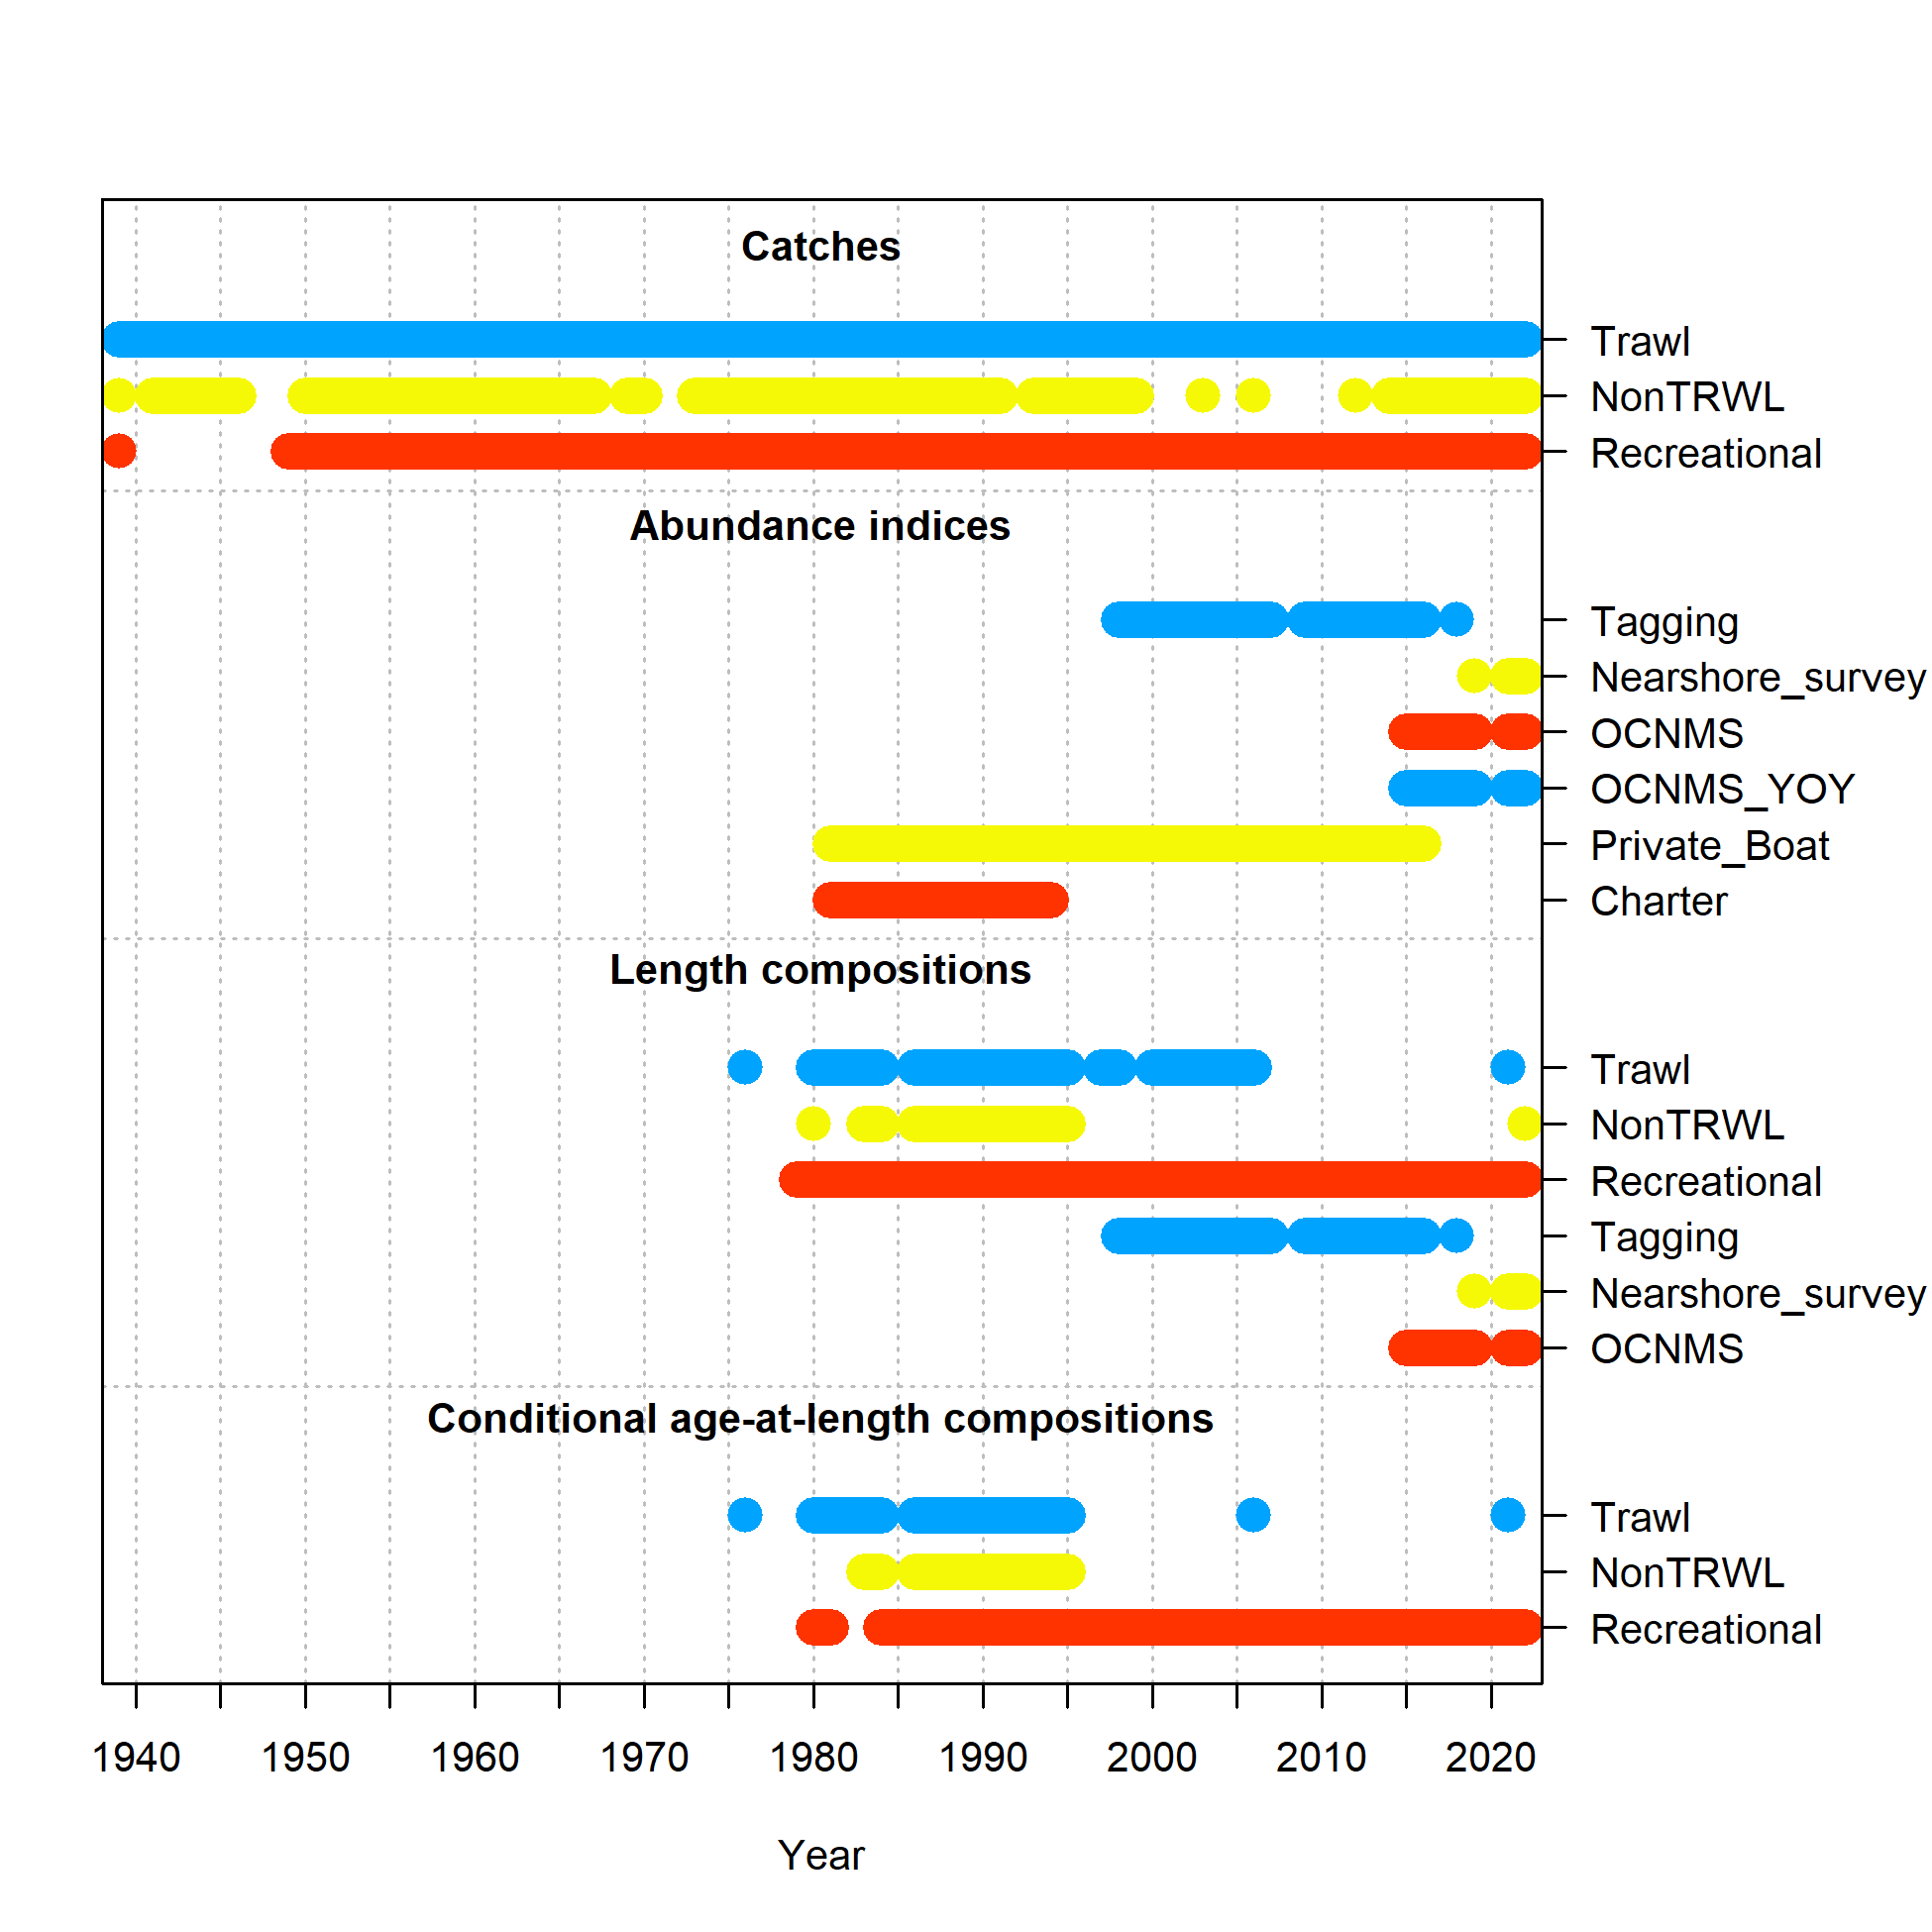
\includegraphics[width=1\textwidth,height=1\textheight]{C:/Users/Jason.Cope/Documents/Github/Sebastes_melanops_WA/Document/models/Reference model/plots/data_plot.png}
\caption{Summary of data sources used in the reference model.\label{fig:data-plot}}
\end{figure}

\begin{figure}
\centering
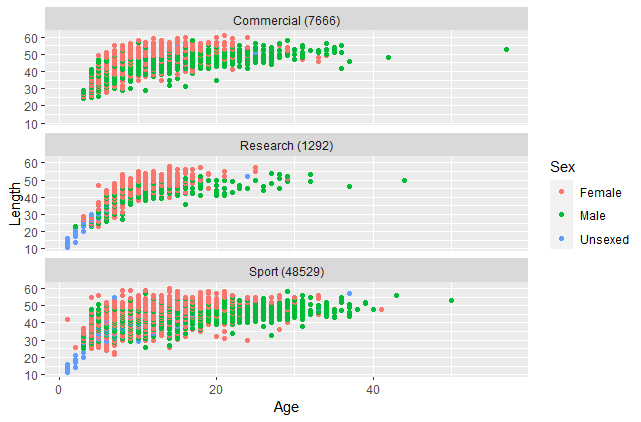
\includegraphics[width=1\textwidth,height=1\textheight]{C:/Users/Jason.Cope/Documents/Github/Sebastes_melanops_WA/Document/figures/biology_plots/WA_AG_Source_Sex.png}
\caption{Observed length-at-age by data source and sex.\label{fig:len-age-data-sex}}
\end{figure}

\begin{figure}
\centering
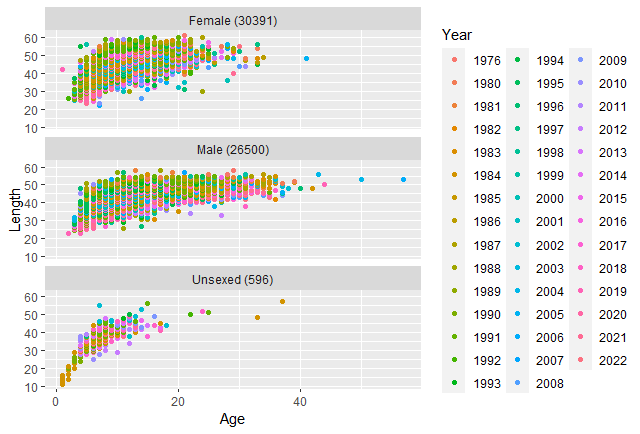
\includegraphics[width=1\textwidth,height=1\textheight]{C:/Users/Jason.Cope/Documents/Github/Sebastes_melanops_WA/Document/figures/biology_plots/WA_AG_Sex_Year.png}
\caption{Observed length-at-age by sex and year. Total samples are indicated in parentheses.\label{fig:len-age-sex-year}}
\end{figure}

\begin{figure}
\centering
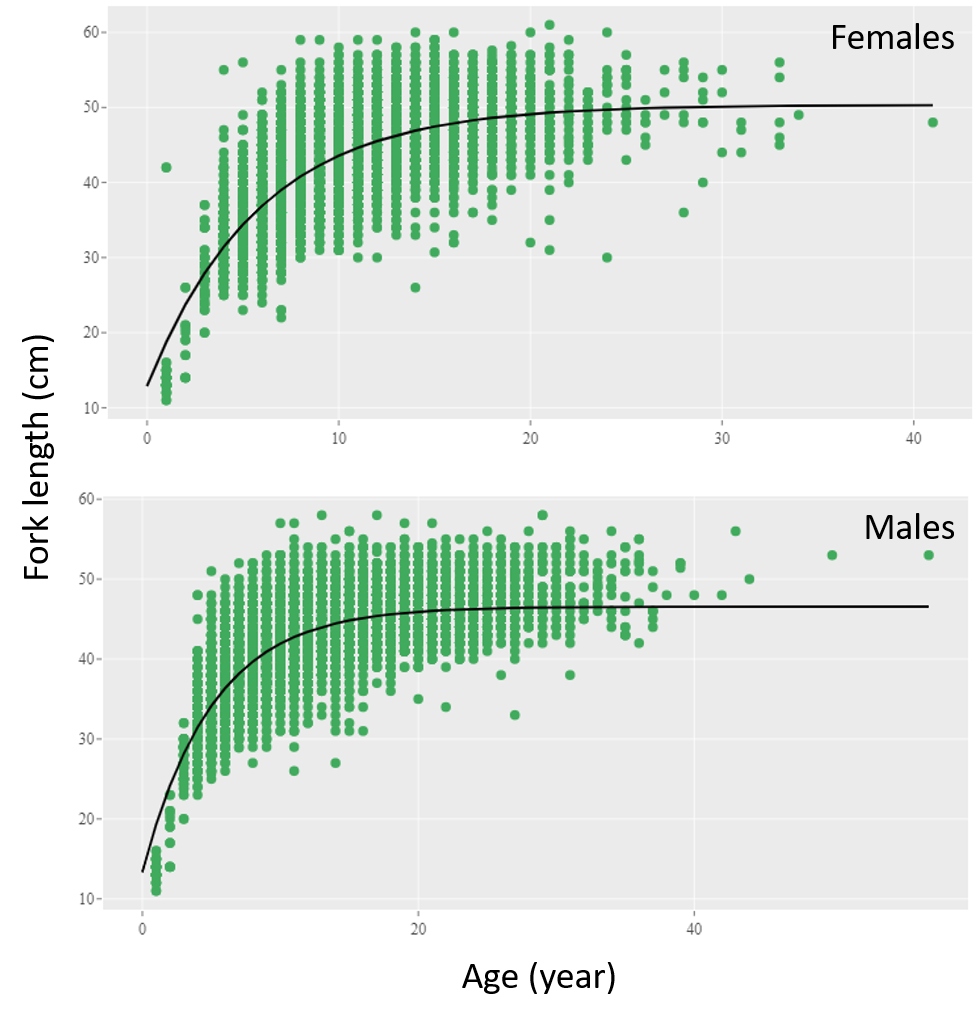
\includegraphics[width=1\textwidth,height=1\textheight]{C:/Users/Jason.Cope/Documents/Github/Sebastes_melanops_WA/Document/figures/biology_plots/WA_VBGF_fit.png}
\caption{External fits to the observed length-at-age by sex.\label{fig:len-age-fit}}
\end{figure}

\begin{figure}
\centering
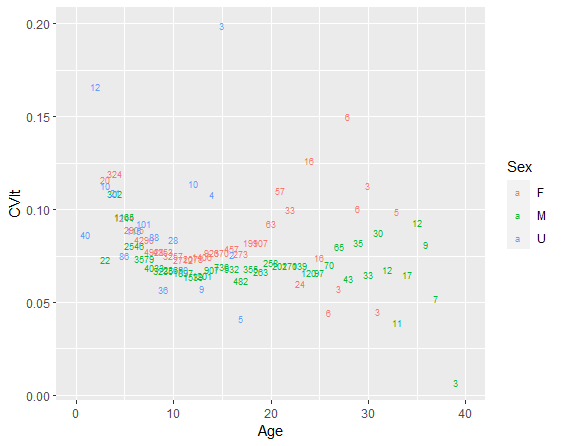
\includegraphics[width=1\textwidth,height=1\textheight]{C:/Users/Jason.Cope/Documents/Github/Sebastes_melanops_WA/Document/figures/biology_plots/WA_CV_Sex_plot.png}
\caption{Coefficient of variation of length by age by sex. Numbers indicate samples by age and colors indicate sex.\label{fig:cv-lt-age}}
\end{figure}

\begin{figure}
\centering
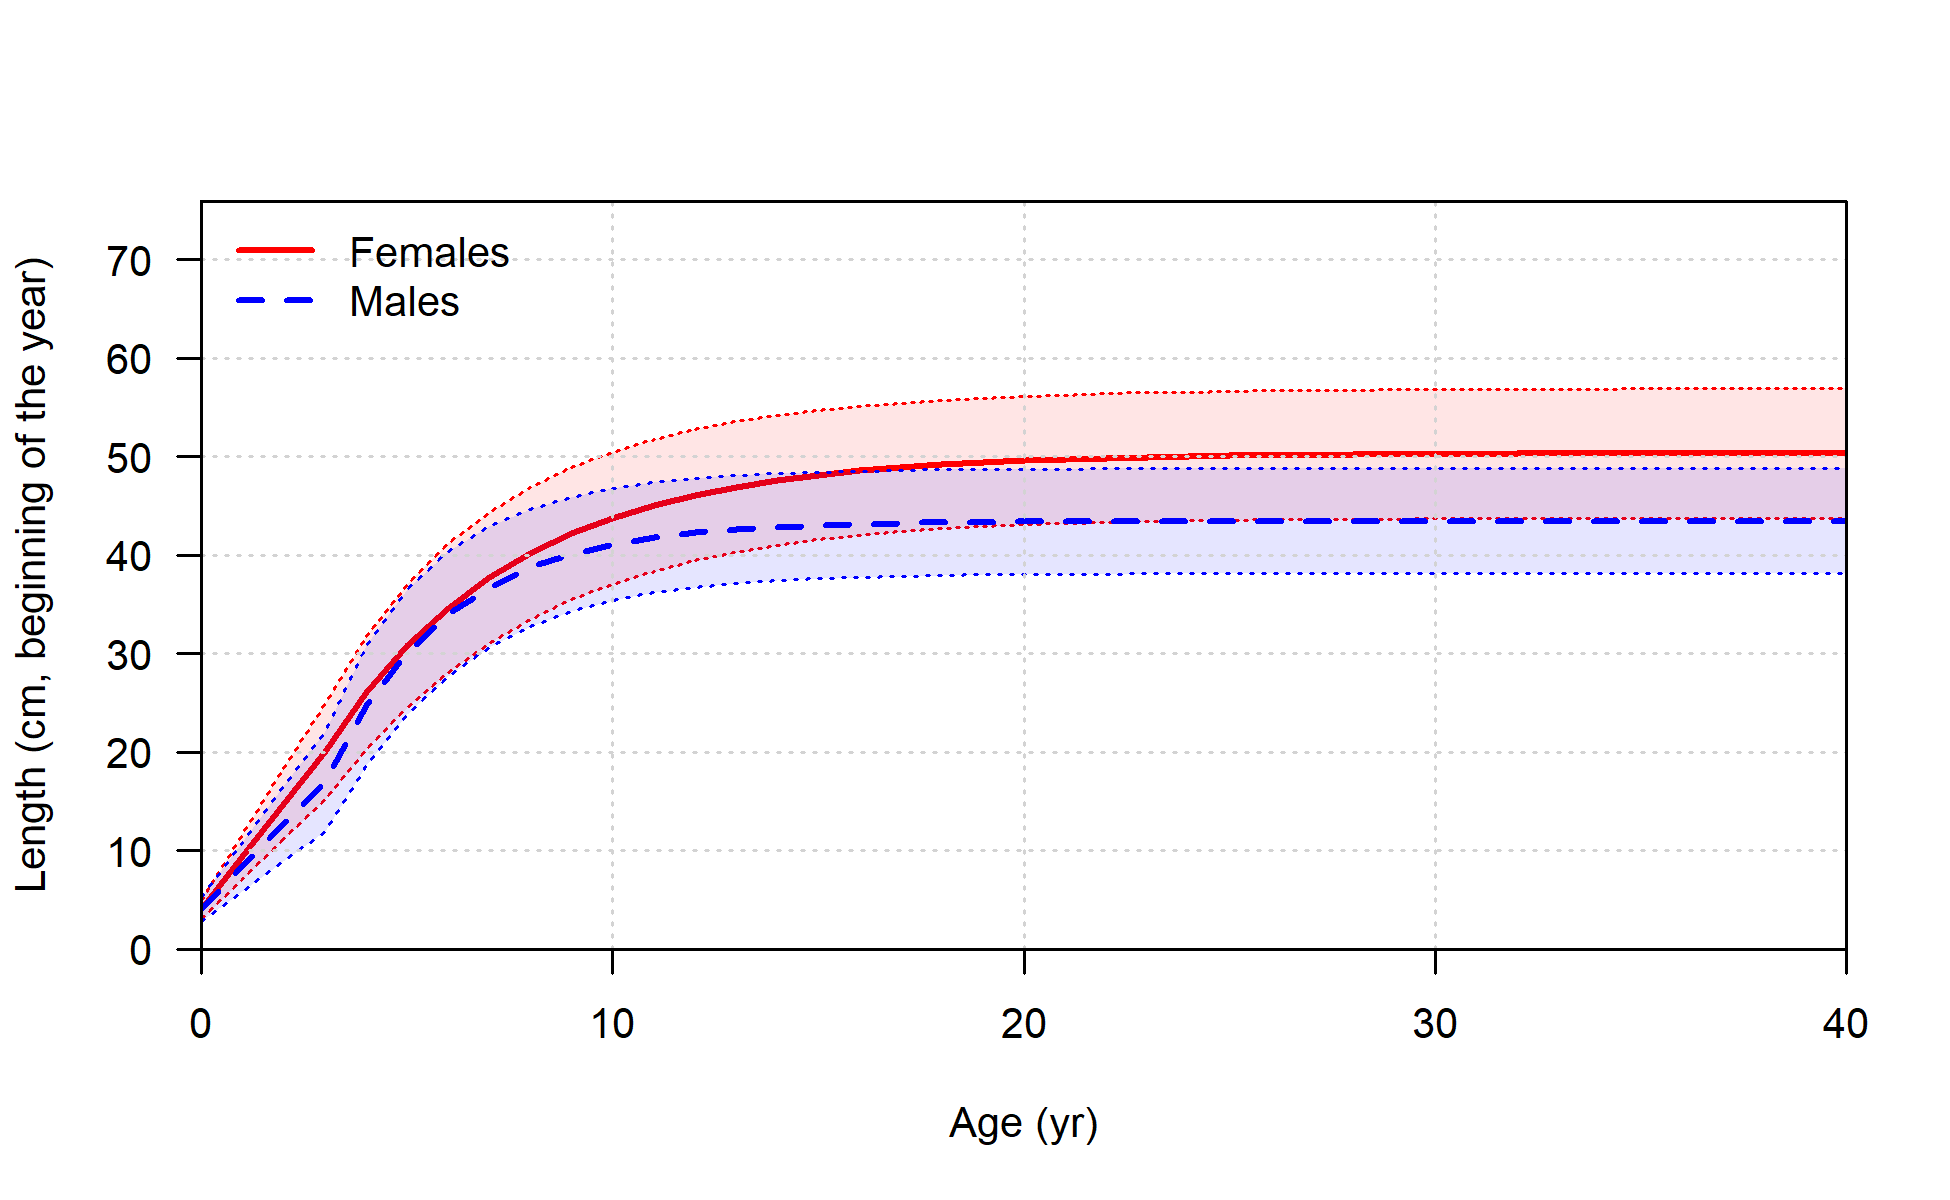
\includegraphics[width=1\textwidth,height=1\textheight]{C:/Users/Jason.Cope/Documents/Github/Sebastes_melanops_WA/Document/models/Reference model/plots/bio1_sizeatage.png}
\caption{Model estimated length-at-age. Shaded area indicates 95 percent distribution of length-at-age around the estimated growth curve.\label{fig:len-age-ss}}
\end{figure}

\clearpage

\begin{figure}
\centering
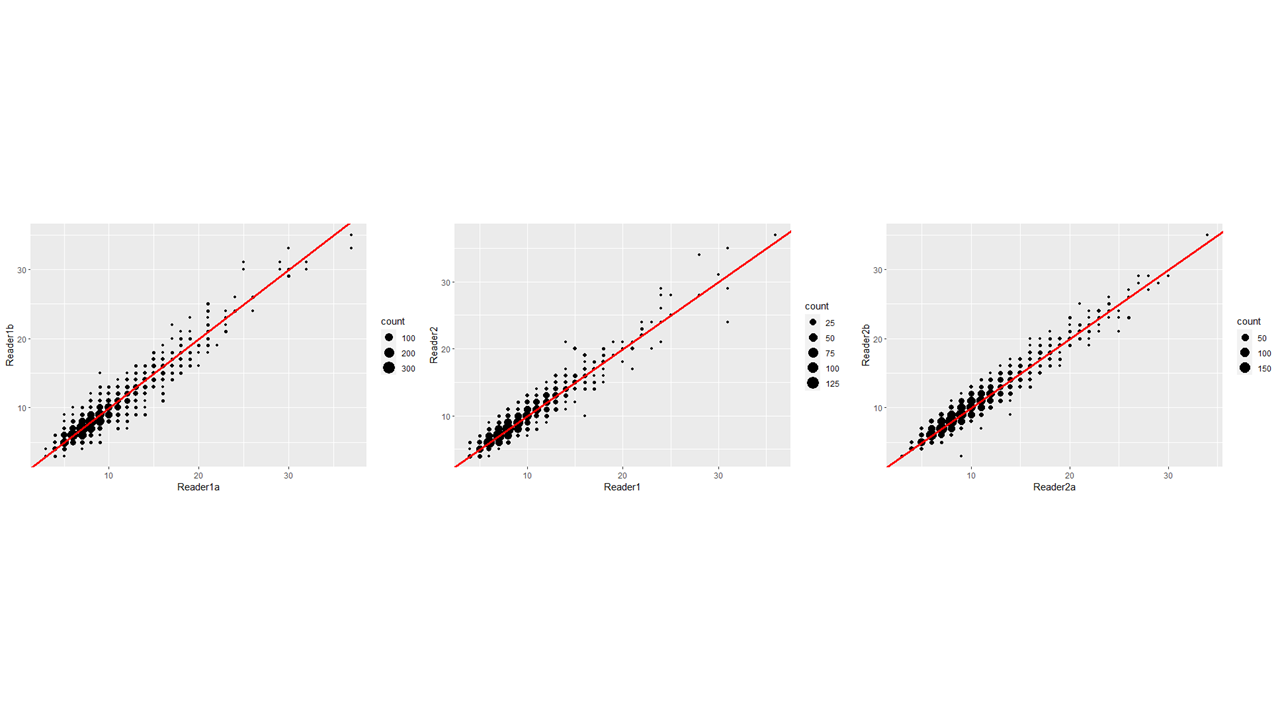
\includegraphics[width=1\textwidth,height=1\textheight]{C:/Users/Jason.Cope/Documents/Github/Sebastes_melanops_WA/Document/figures/biology_plots/Age1_1plots.png}
\caption{Ageing bias plots by reader comparisons.\label{fig:age-bias_plot}}
\end{figure}

\begin{figure}
\centering
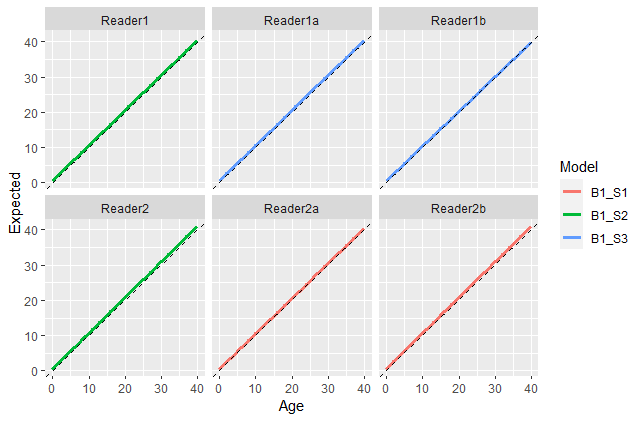
\includegraphics[width=1\textwidth,height=1\textheight]{C:/Users/Jason.Cope/Documents/Github/Sebastes_melanops_WA/Document/figures/biology_plots/WA_Reader_Bias_plot.png}
\caption{Estimated bias relationships for each considered matrix. Reader 1 is always considered unbiased. Reader 1a and 1b is an intra-reader comparison. B refers to the bias type and S refers to the imprecision type in the model selection for the ageing error matrix.\label{fig:age-error-bias}}
\end{figure}

\begin{figure}
\centering
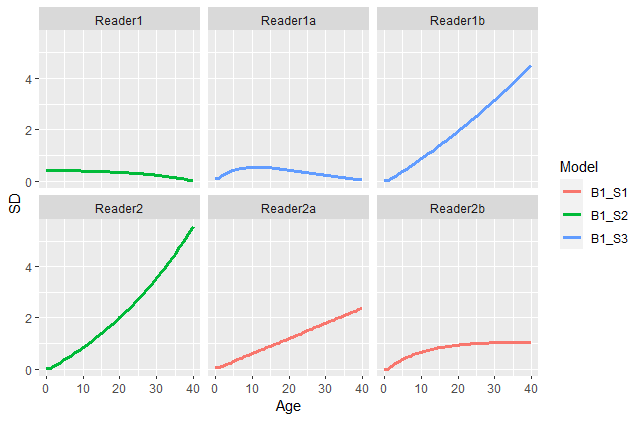
\includegraphics[width=1\textwidth,height=1\textheight]{C:/Users/Jason.Cope/Documents/Github/Sebastes_melanops_WA/Document/figures/biology_plots/WA_Reader_SD_plot.png}
\caption{Ageing error matrix standard deviation (SD) values by comparison. B refers to the bias type and S refers to the imprecision type in the model selection for the ageing error matrix.\label{fig:age-error-sd}}
\end{figure}

\begin{figure}
\centering
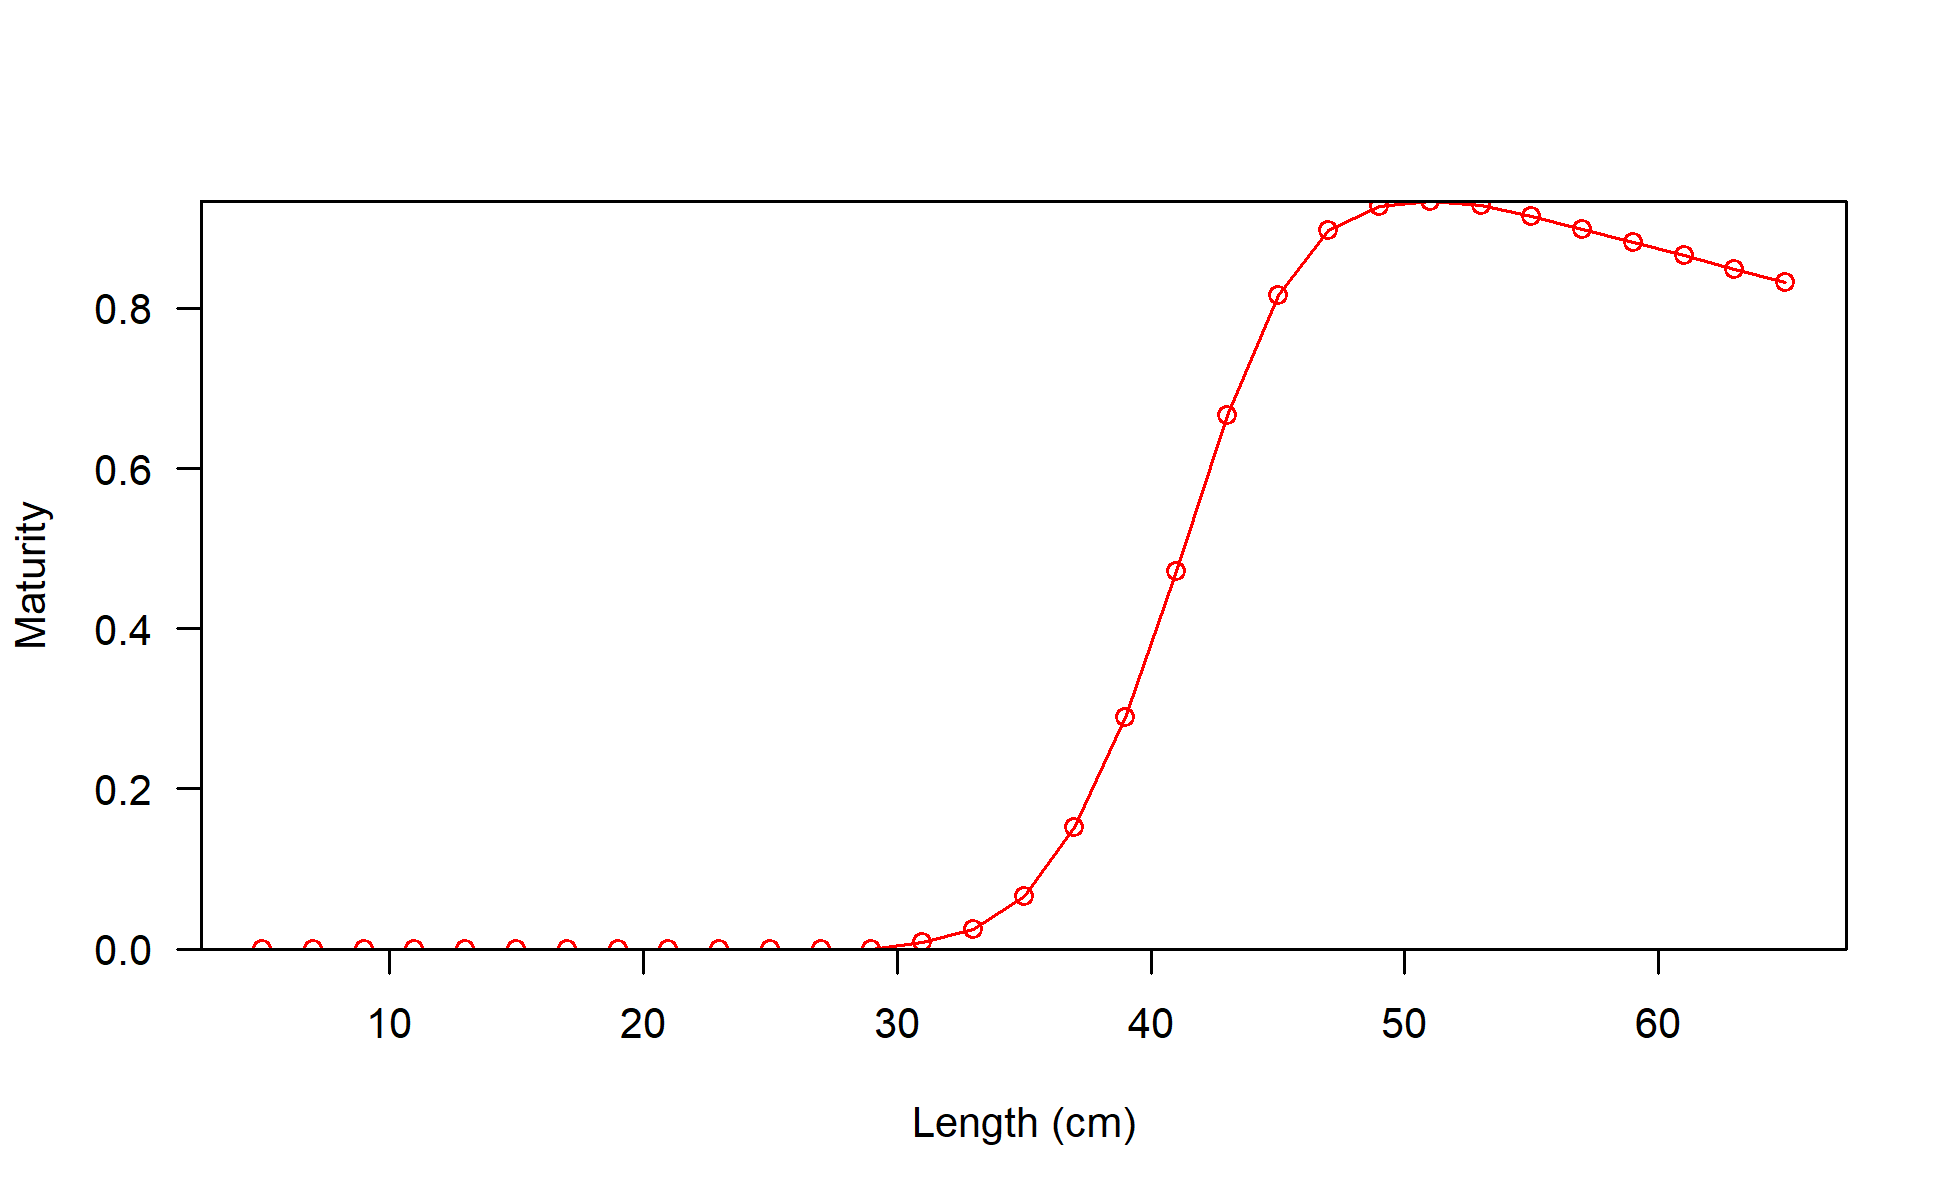
\includegraphics[width=1\textwidth,height=1\textheight]{C:/Users/Jason.Cope/Documents/Github/Sebastes_melanops_WA/Document/models/Reference model/plots/bio6_maturity.png}
\caption{Maturity as a function of length (cm).\label{fig:maturity}}
\end{figure}

\begin{figure}
\centering
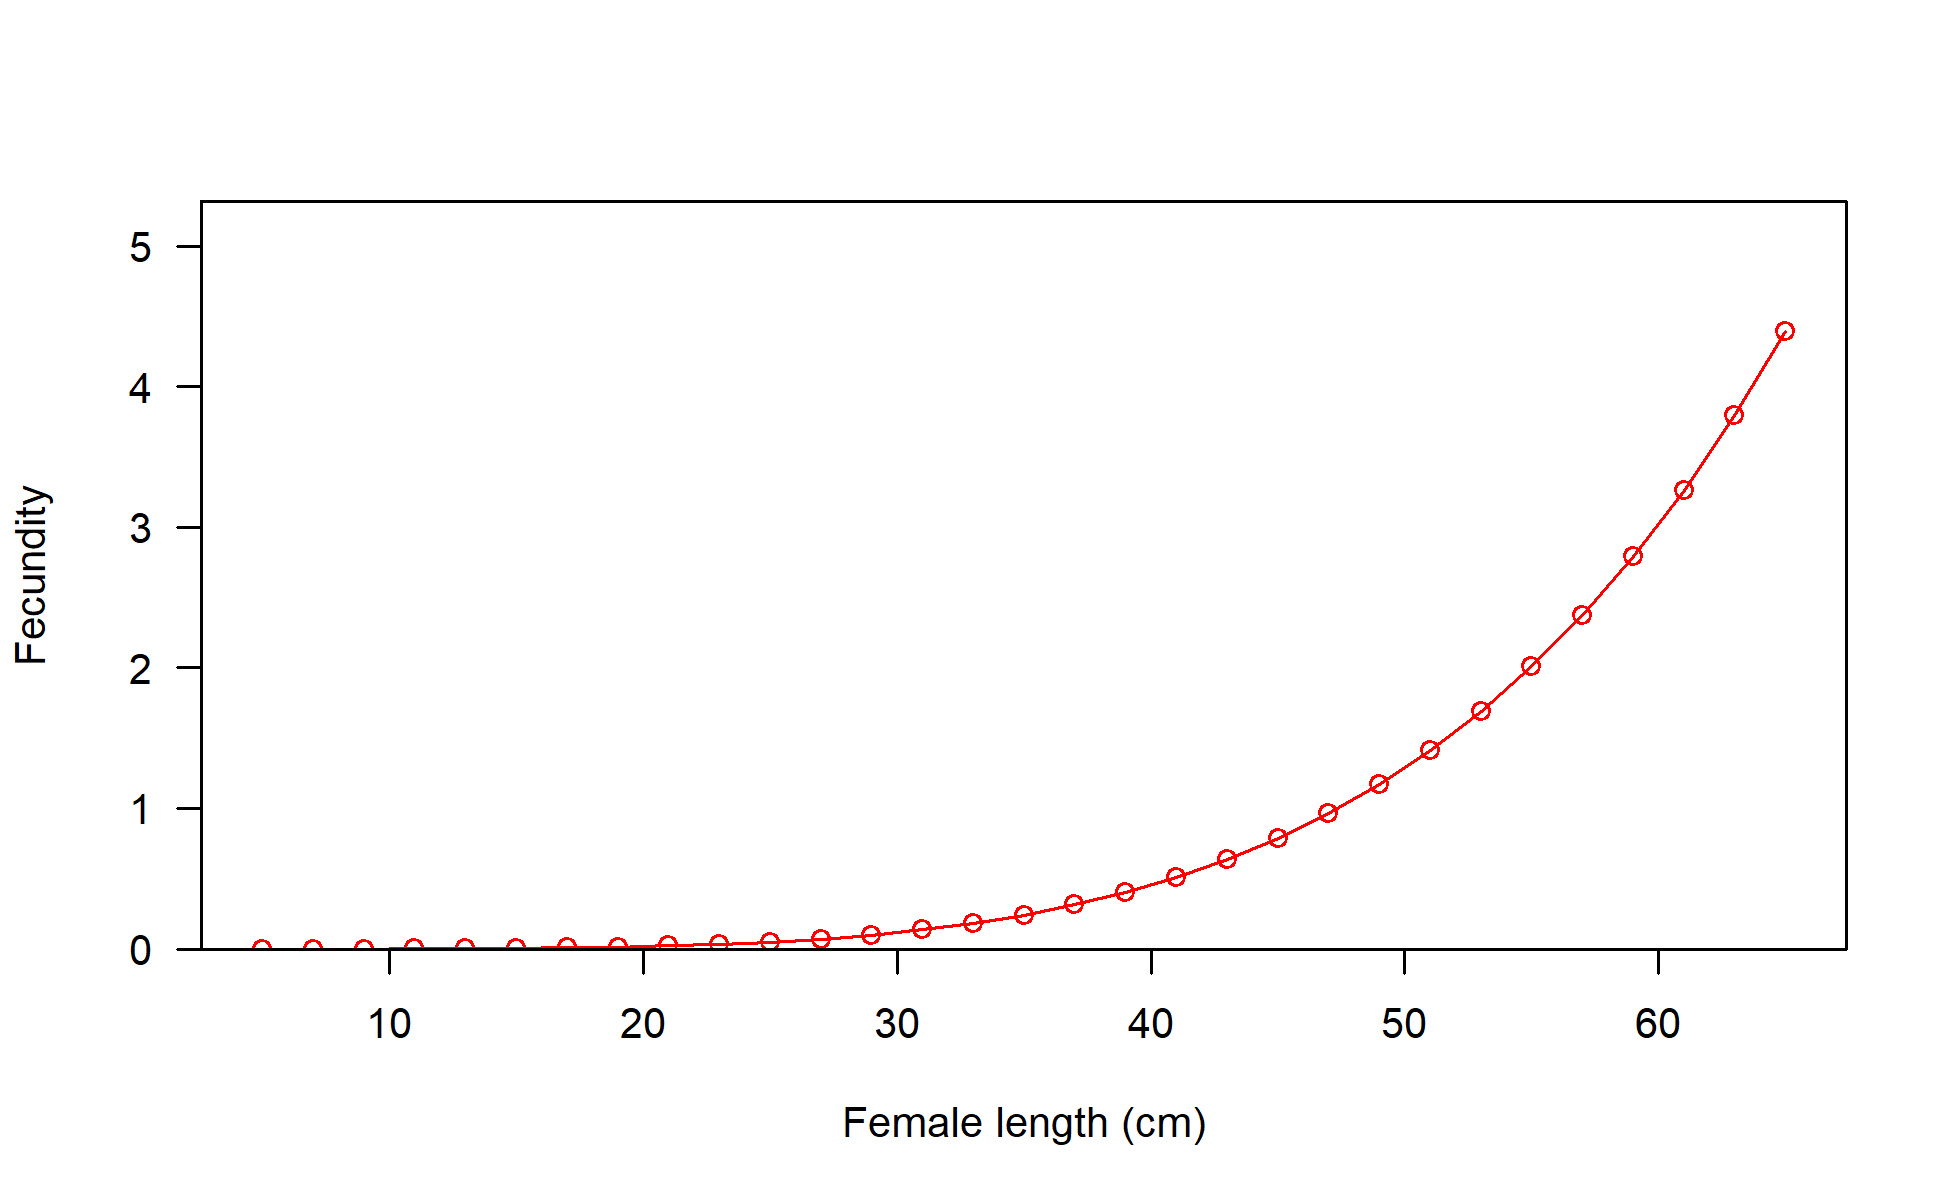
\includegraphics[width=1\textwidth,height=1\textheight]{C:/Users/Jason.Cope/Documents/Github/Sebastes_melanops_WA/Document/models/Reference model/plots/bio9_fecundity_len.png}
\caption{Fecundity (kg) as a function of length (cm).\label{fig:fecundity}}
\end{figure}

\begin{figure}
\centering
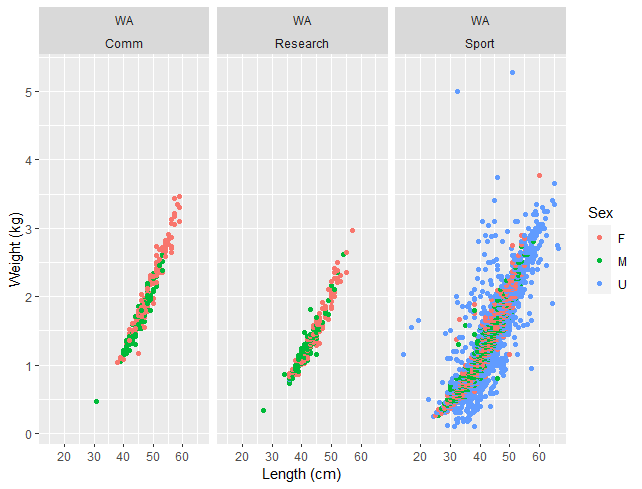
\includegraphics[width=1\textwidth,height=1\textheight]{C:/Users/Jason.Cope/Documents/Github/Sebastes_melanops_WA/Document/figures/biology_plots/LW_WA_State_Source_Sex.png}
\caption{Sex-specific length (cm)-weight (kg) data for black rockfish samples by source.\label{fig:len-weight-data}}
\end{figure}

\begin{figure}
\centering
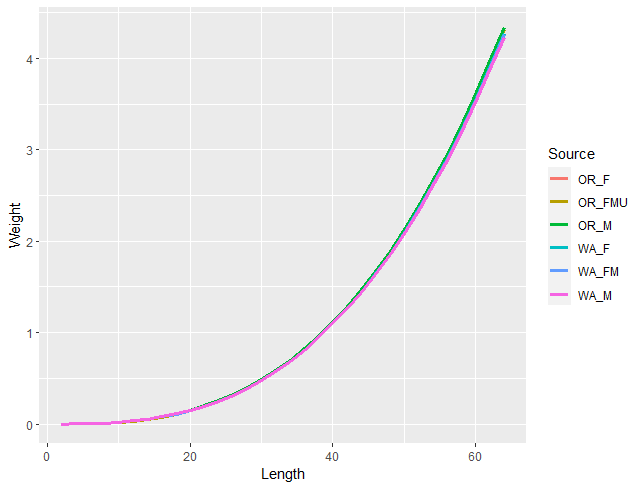
\includegraphics[width=1\textwidth,height=1\textheight]{C:/Users/Jason.Cope/Documents/Github/Sebastes_melanops_WA/Document/figures/biology_plots/LW_lines_States_Sex.png}
\caption{Sex-specific length (cm)-weight (kg) estimated power function relationships. Washington state estimate relationships are also provided for comparison.\label{fig:len-weight-or-wa}}
\end{figure}

\clearpage

\begin{figure}
\centering
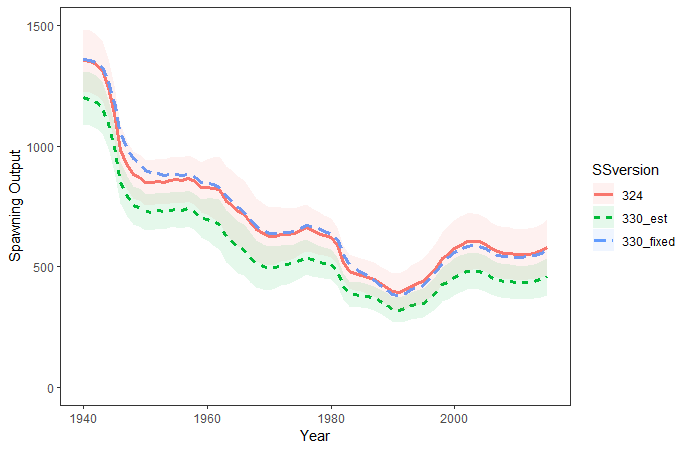
\includegraphics[width=1\textwidth,height=1\textheight]{C:/Users/Jason.Cope/Documents/Github/Sebastes_melanops_WA/Document/figures/Bridge/WA_SB_comp_plot.png}
\caption{Comparison of spawning output for black rockfish in waters off of Washington between Stock Synthesis versions 3.24 and 3.30. Uncertainty envelops are 95\% confidence intervals.\label{fig:ssb_bridge_comps}}
\end{figure}

\begin{figure}
\centering
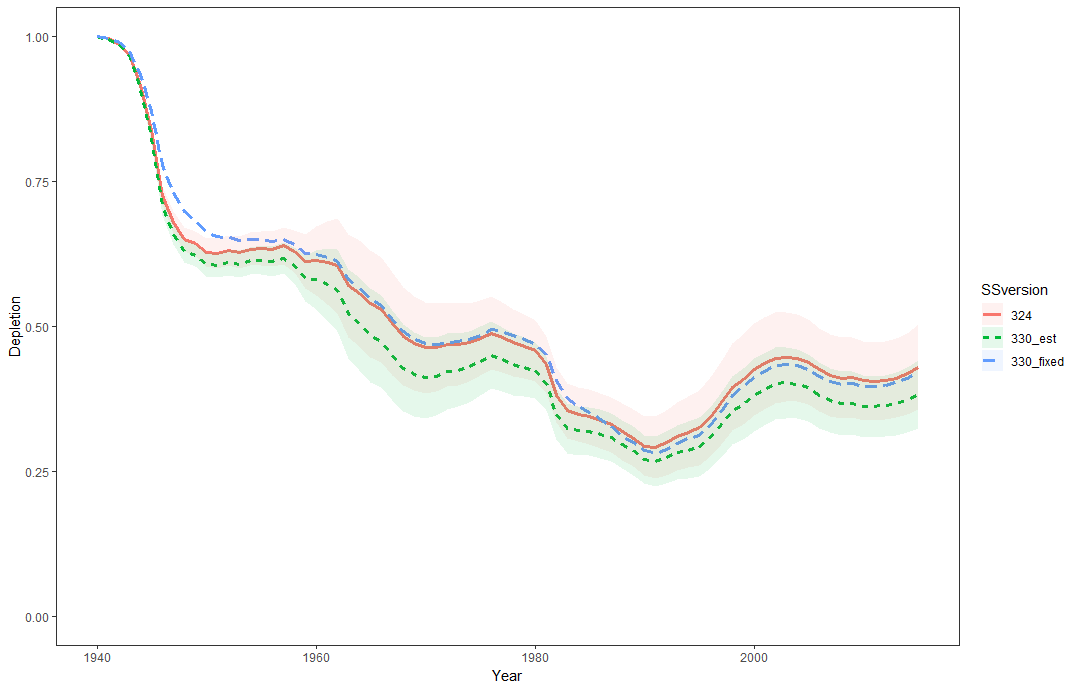
\includegraphics[width=1\textwidth,height=1\textheight]{C:/Users/Jason.Cope/Documents/Github/Sebastes_melanops_WA/Document/figures/Bridge/WA_Dep_comp_plot.png}
\caption{Comparison of spawning output for black rockfish in waters off of Washington between Stock Synthesis versions 3.24 and 3.30. Uncertainty envelops are 95\% confidence intervals.\label{fig:deps_bridge_comps}}
\end{figure}

\clearpage

\hypertarget{app-a}{%
\section{Appendix A: Detailed Fit to Length Composition Data}\label{app-a}}

\begin{figure}
\centering
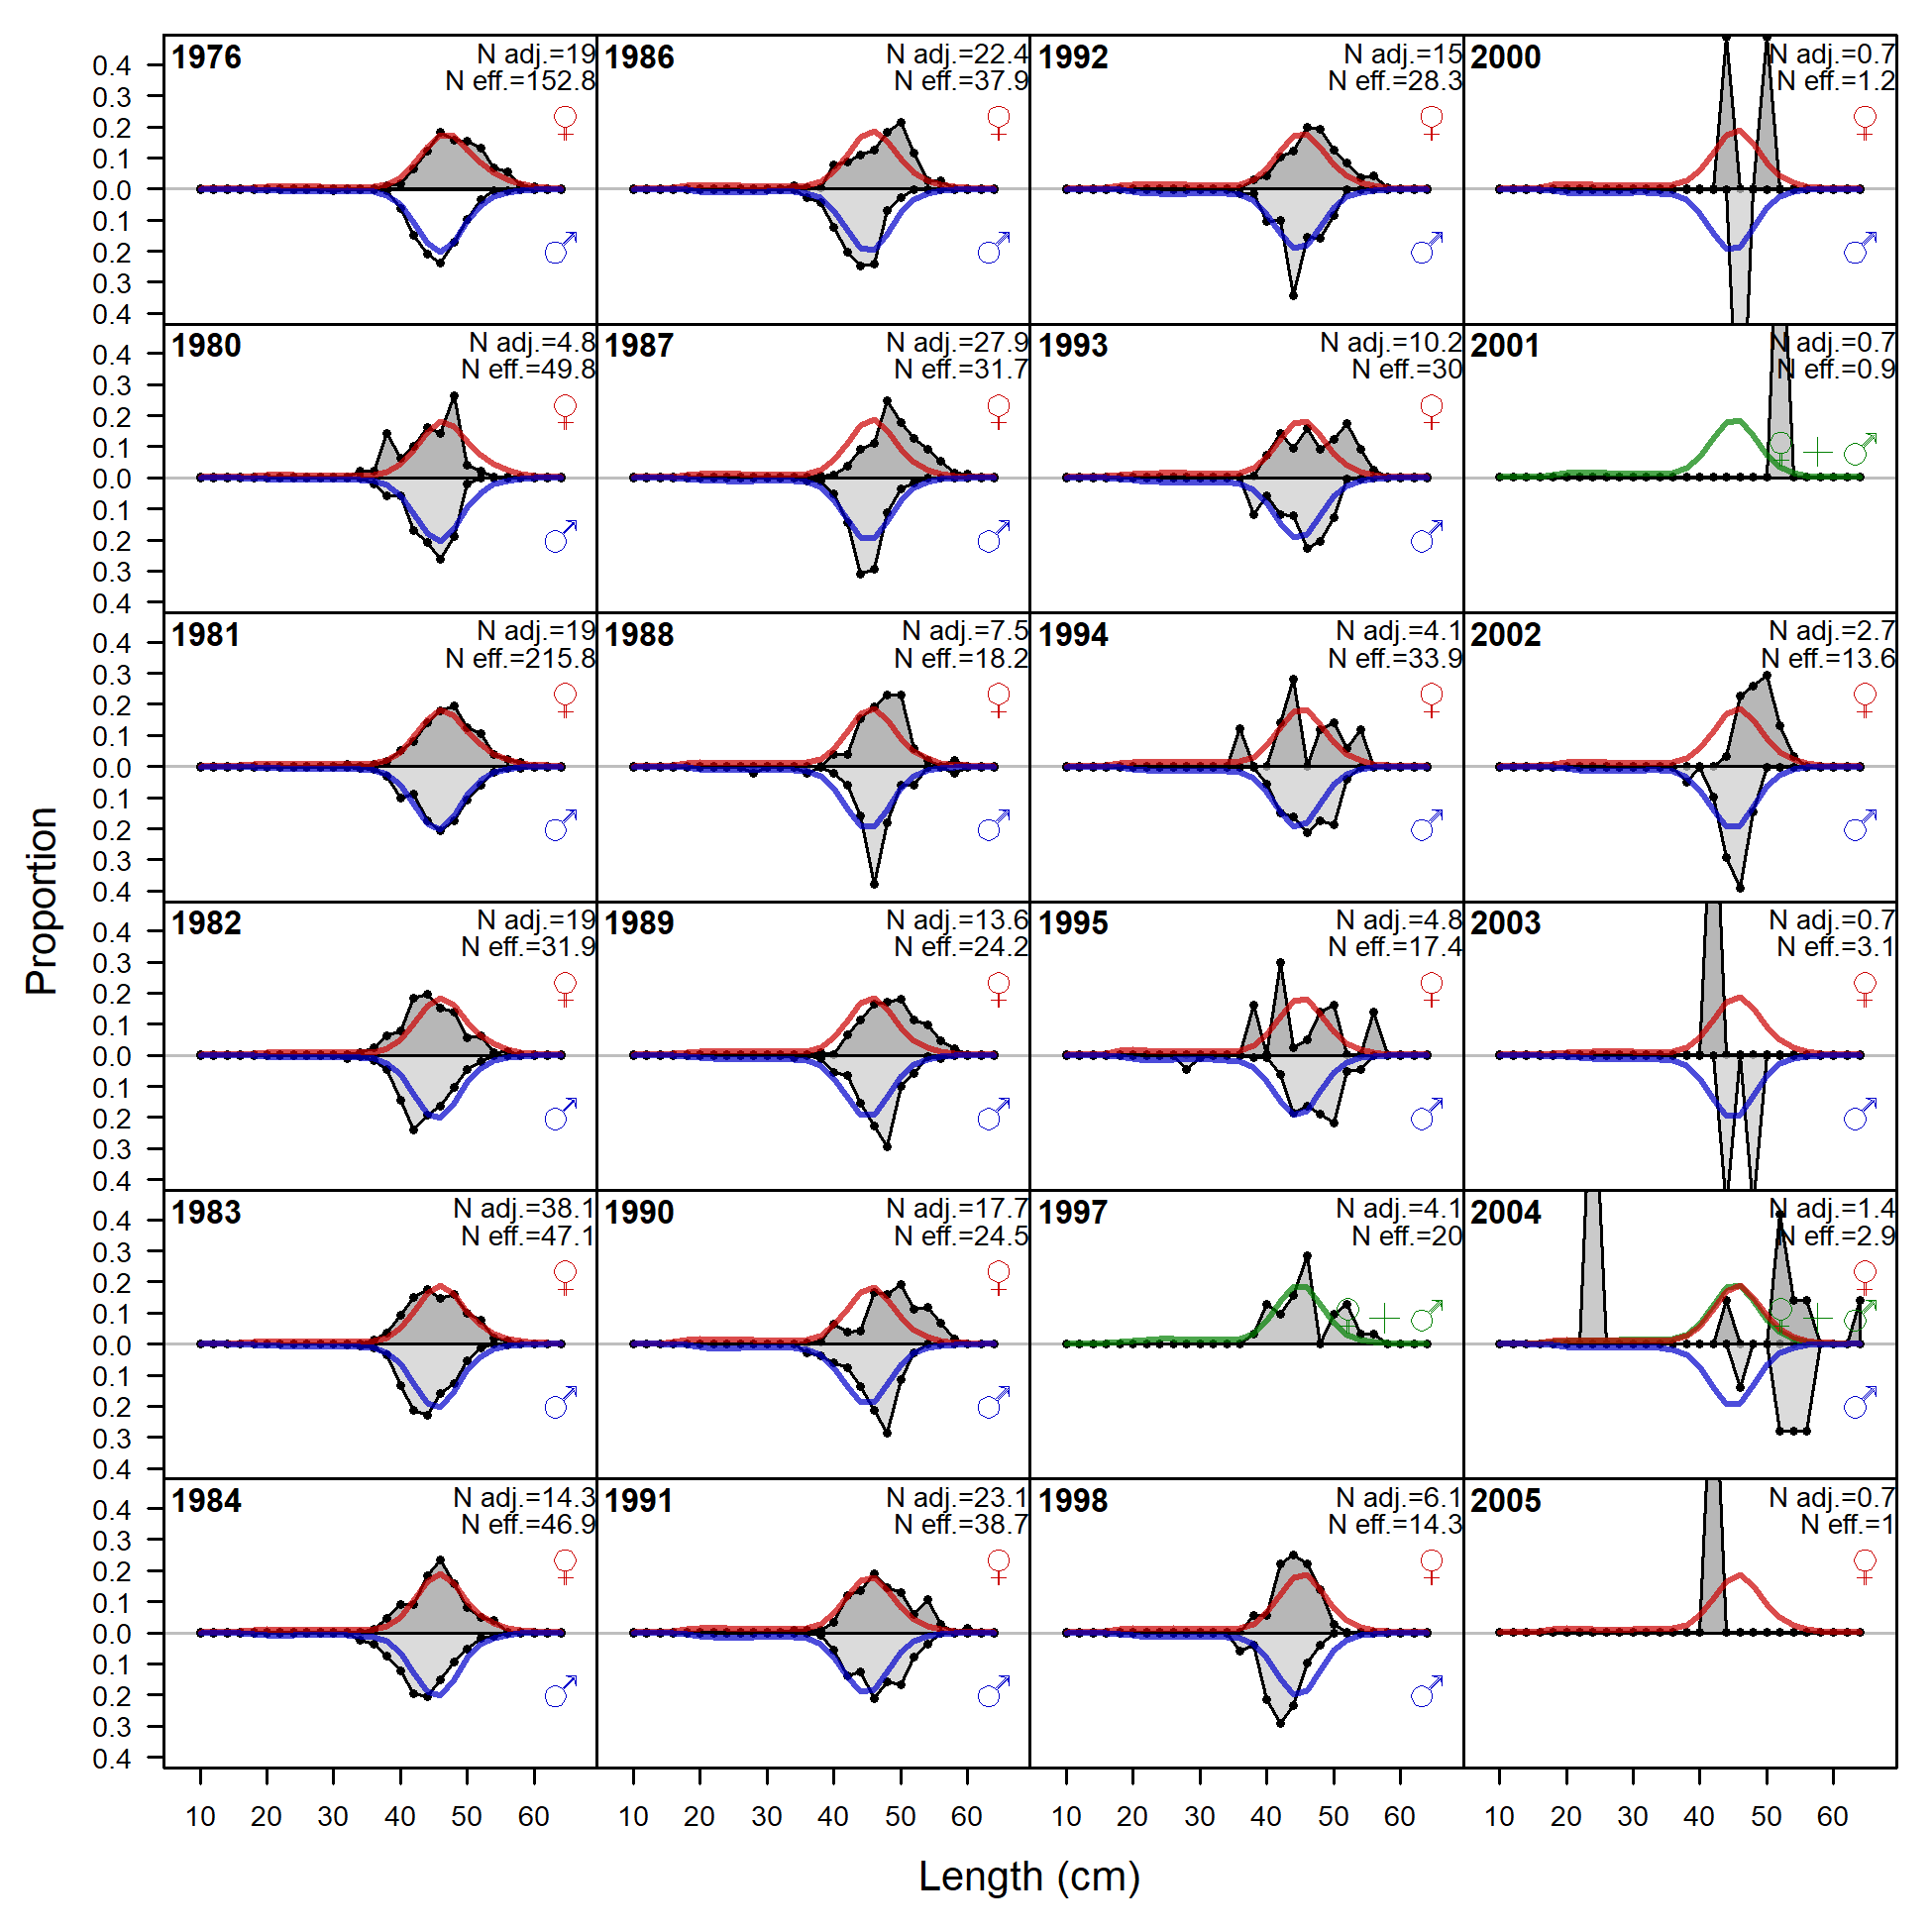
\includegraphics[width=1\textwidth,height=1\textheight]{C:/Users/Jason.Cope/Documents/Github/Sebastes_melanops_WA/Document/models/Reference model/plots/comp_lenfit_flt1mkt0_page1.png}
\caption{Length comps, whole catch, Trawl (plot 1 of 2).`N adj.' is the input sample size after data-weighting adjustment. N eff. is the calculated effective sample size used in the McAllister-Ianelli tuning method.\label{fig:comp_lenfit_flt1mkt0_page1}}
\end{figure}

\begin{figure}
\centering
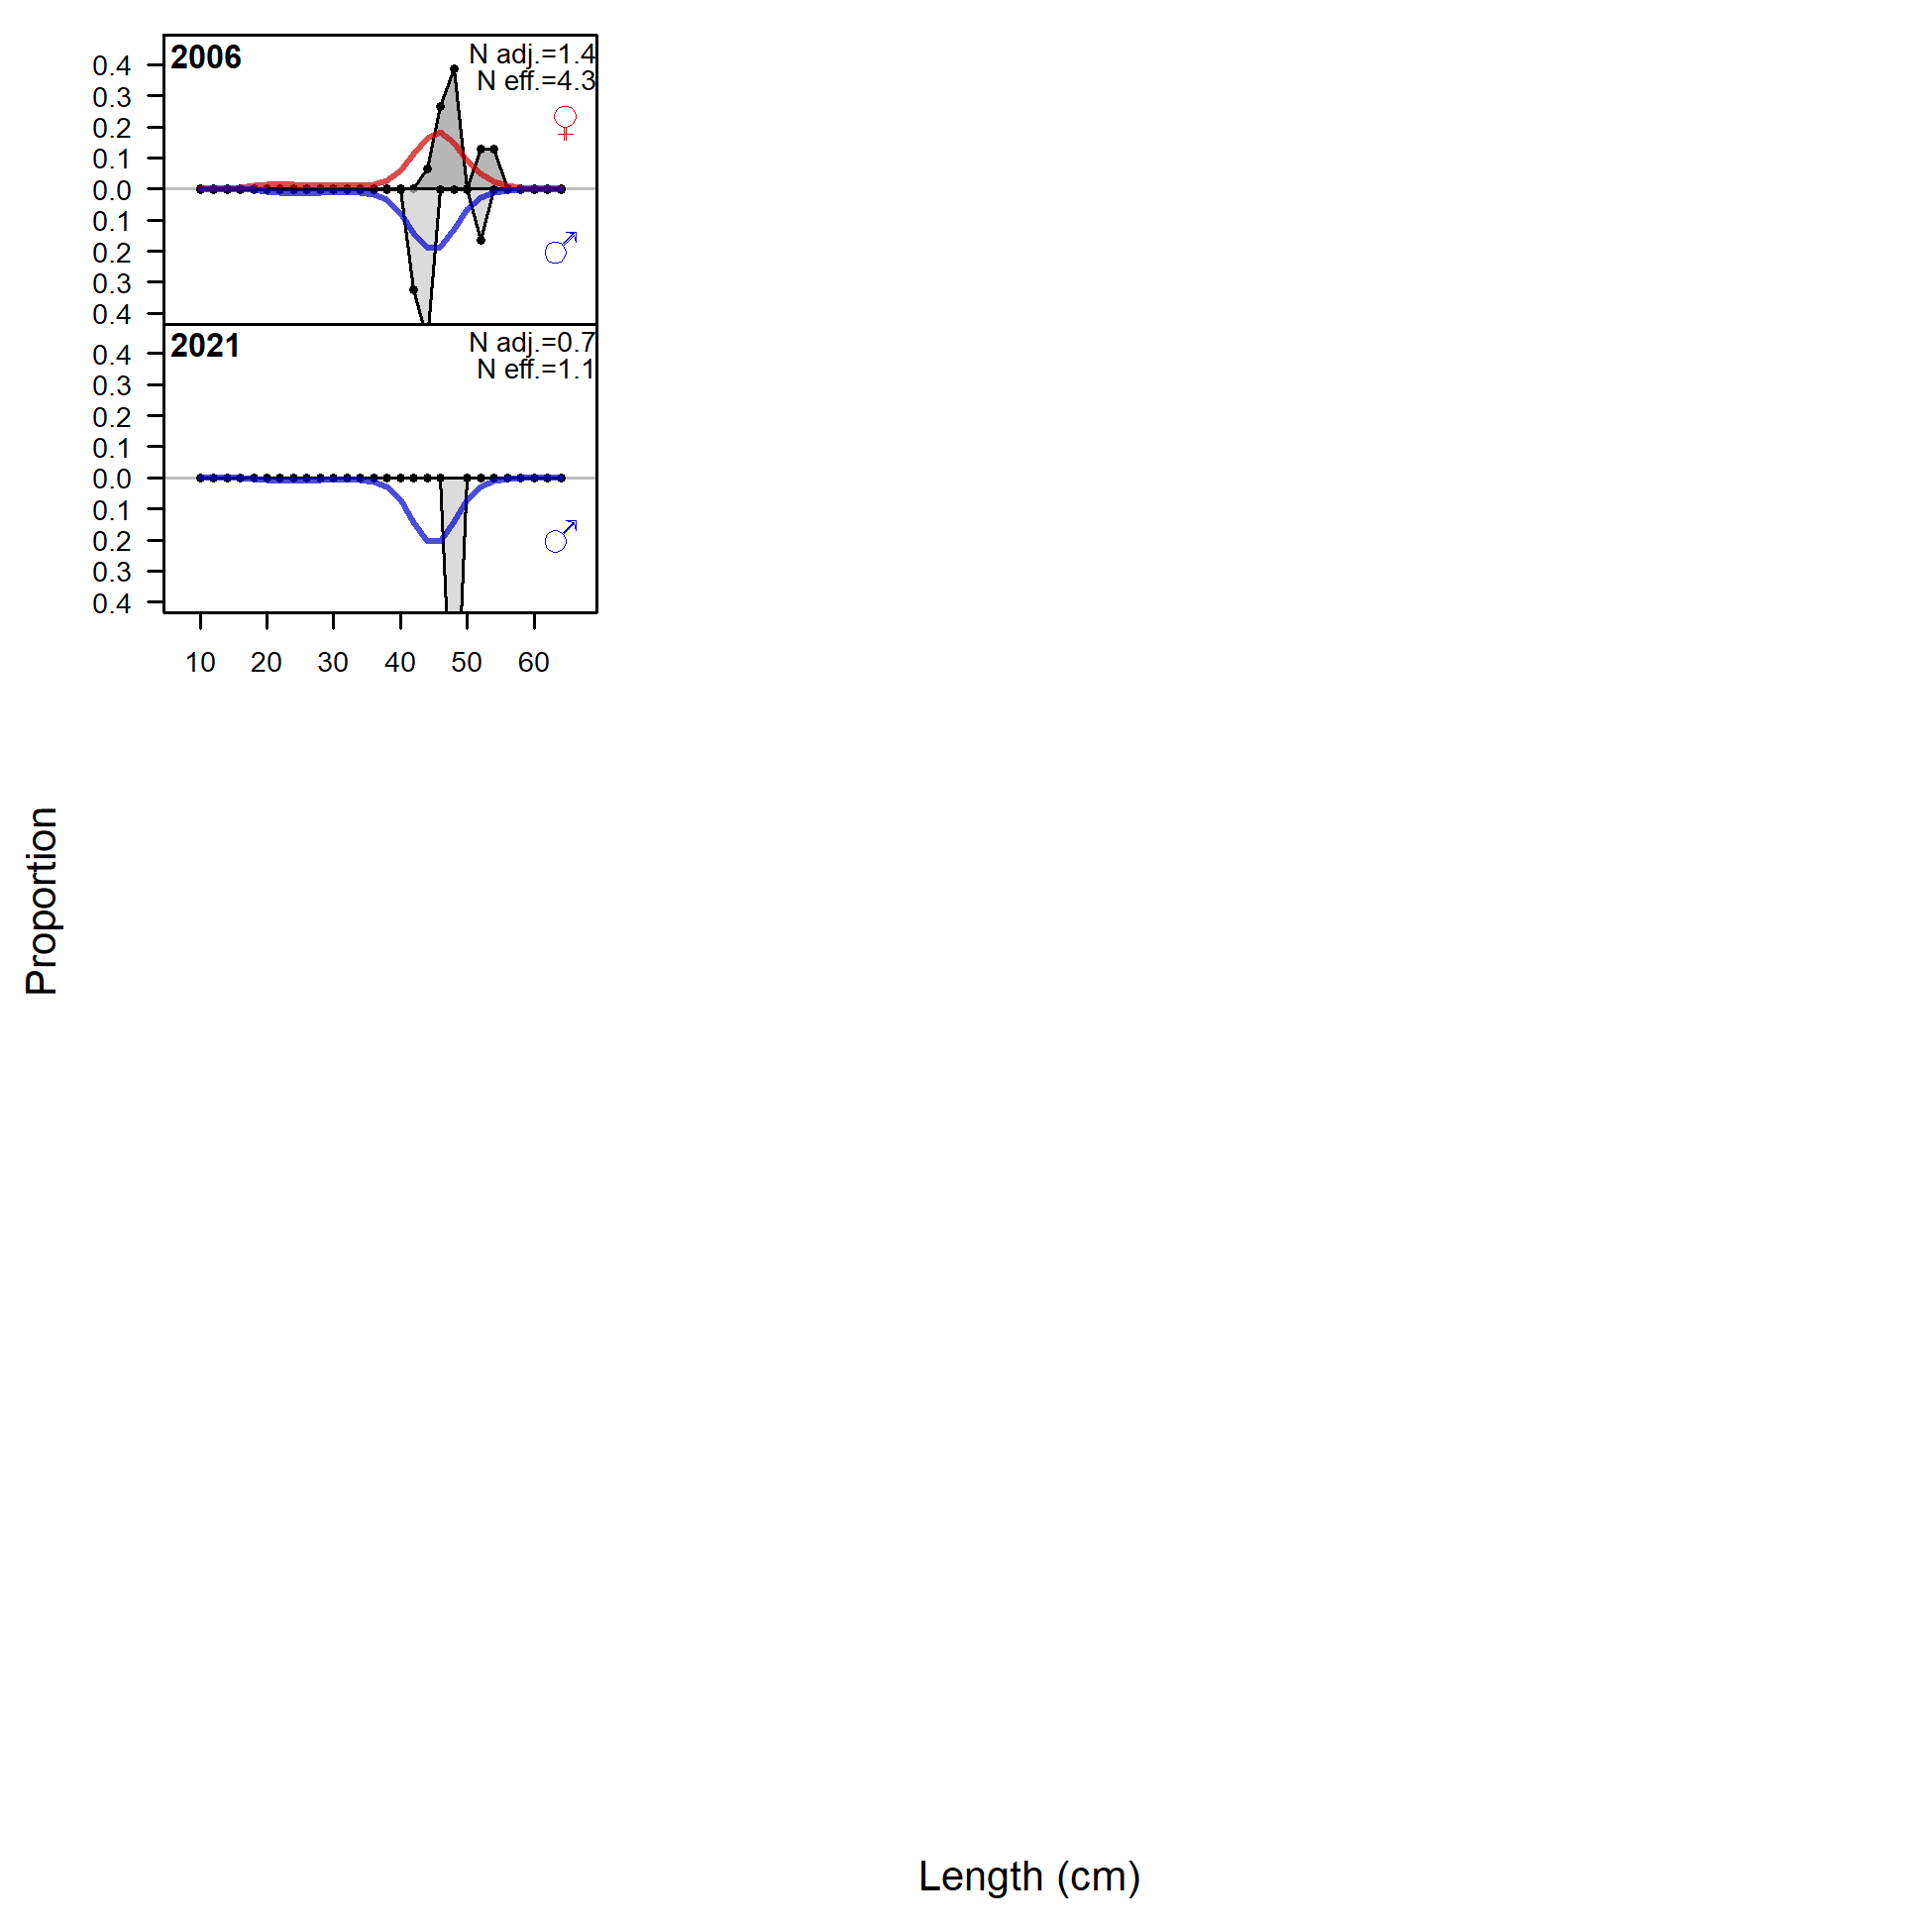
\includegraphics[width=1\textwidth,height=1\textheight]{C:/Users/Jason.Cope/Documents/Github/Sebastes_melanops_WA/Document/models/Reference model/plots/comp_lenfit_flt1mkt0_page2.png}
\caption{Length comps, whole catch, Trawl (plot 1 of 2).`N adj.' is the input sample size after data-weighting adjustment. N eff. is the calculated effective sample size used in the McAllister-Ianelli tuning method. (plot 2 of 2).\label{fig:comp_lenfit_flt1mkt0_page2}}
\end{figure}

\begin{figure}
\centering
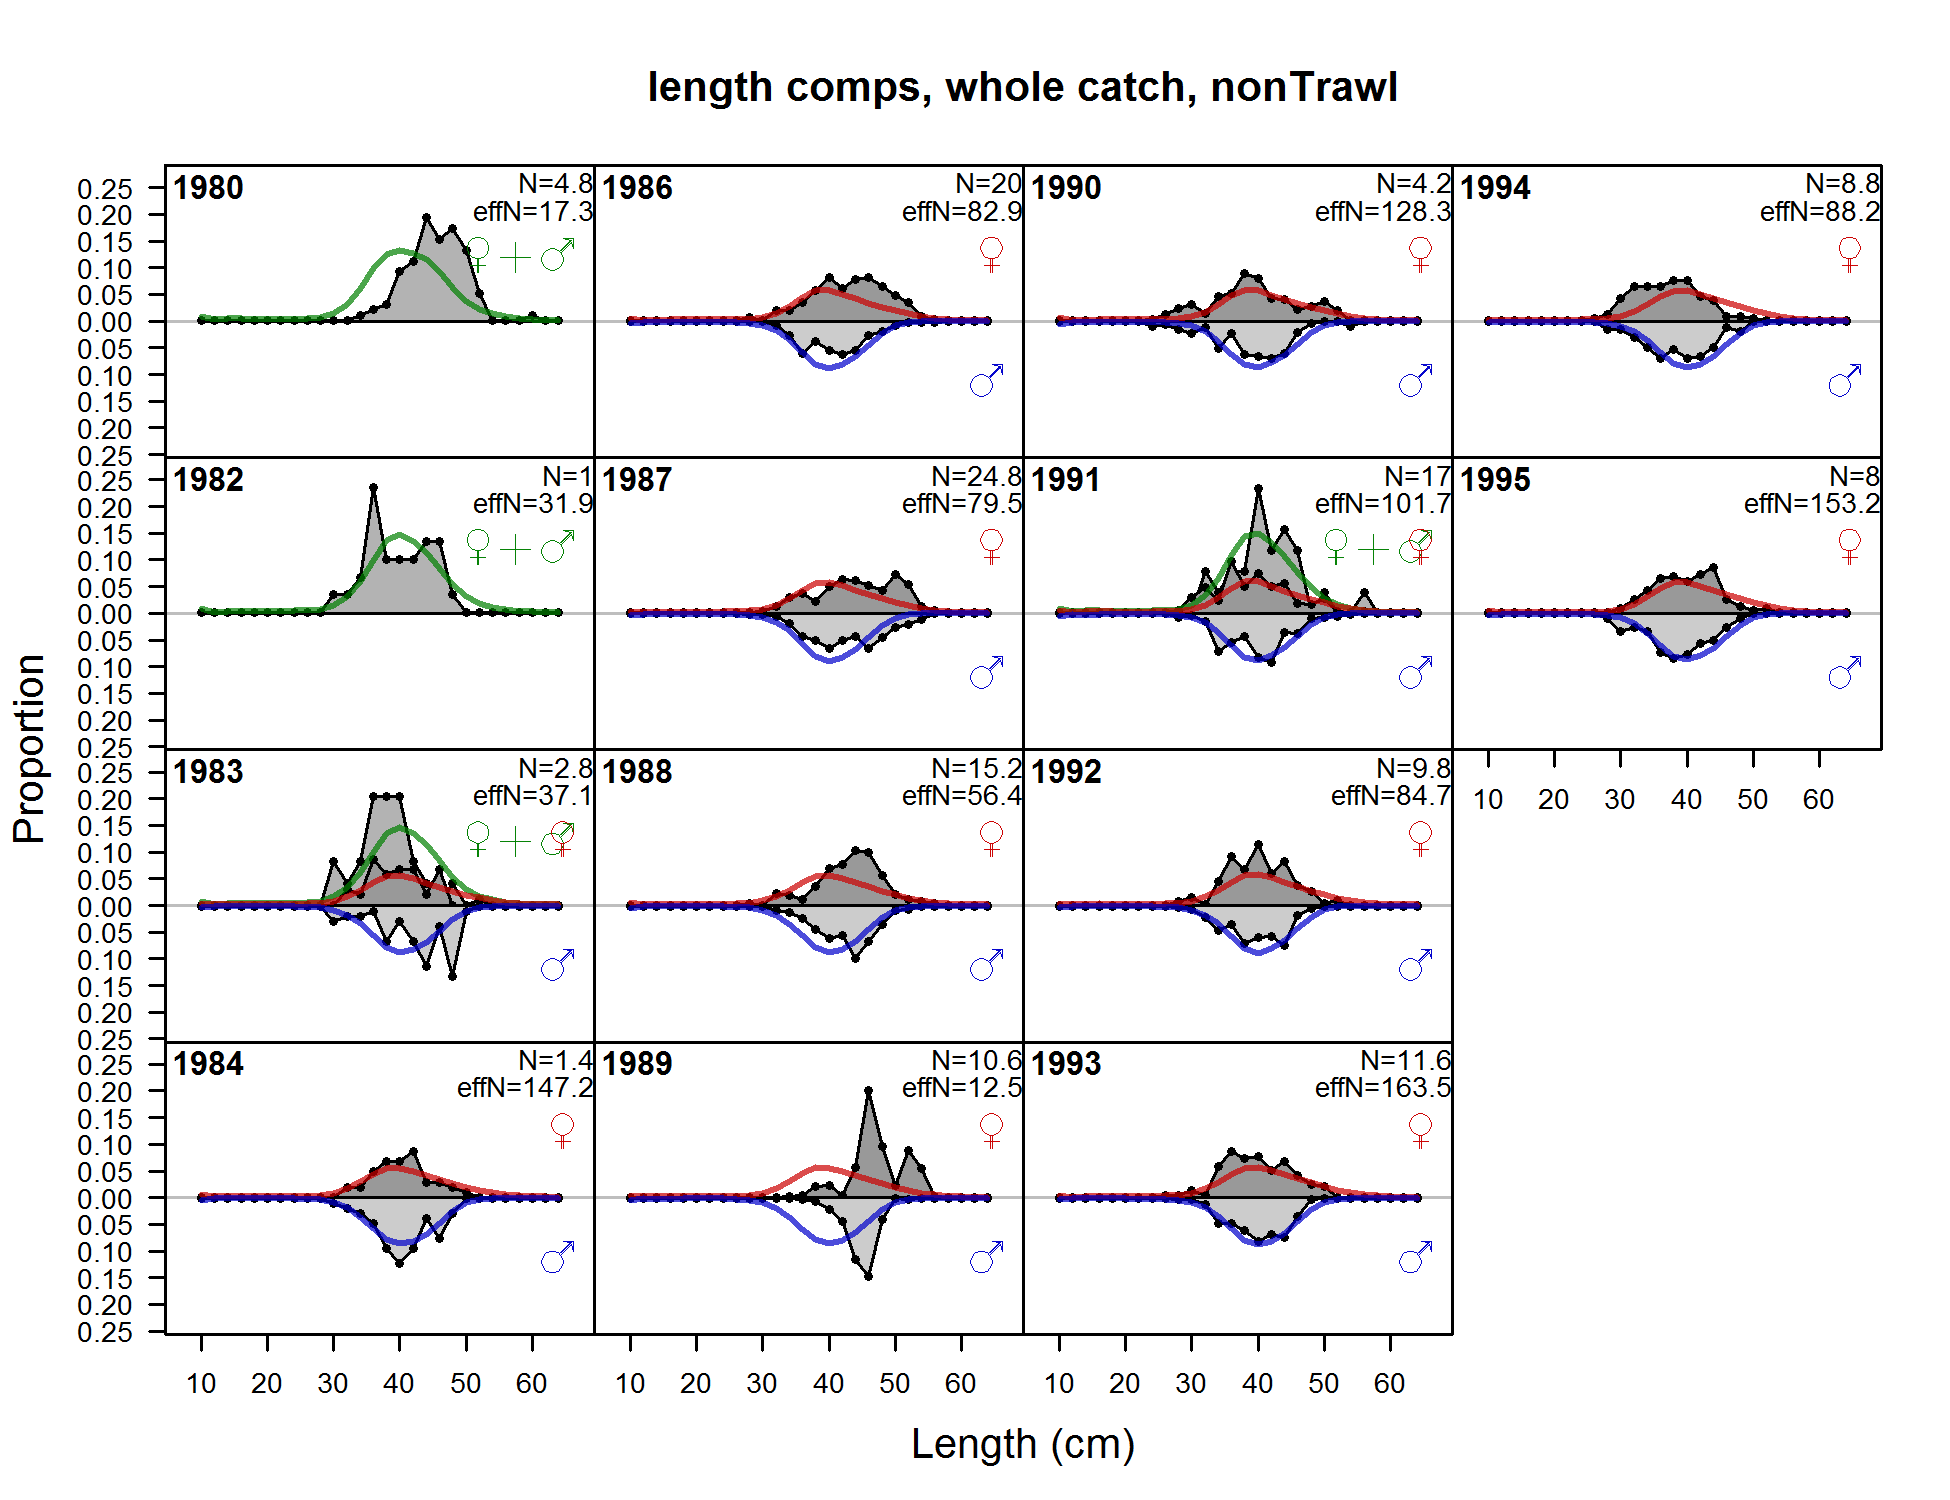
\includegraphics[width=1\textwidth,height=1\textheight]{C:/Users/Jason.Cope/Documents/Github/Sebastes_melanops_WA/Document/models/Reference model/plots/comp_lenfit_flt2mkt0.png}
\caption{Length comps, whole catch, NonTRWL.`N adj.' is the input sample size after data-weighting adjustment. N eff. is the calculated effective sample size used in the McAllister-Ianelli tuning method.\label{fig:comp_lenfit_flt2mkt0}}
\end{figure}

\begin{figure}
\centering
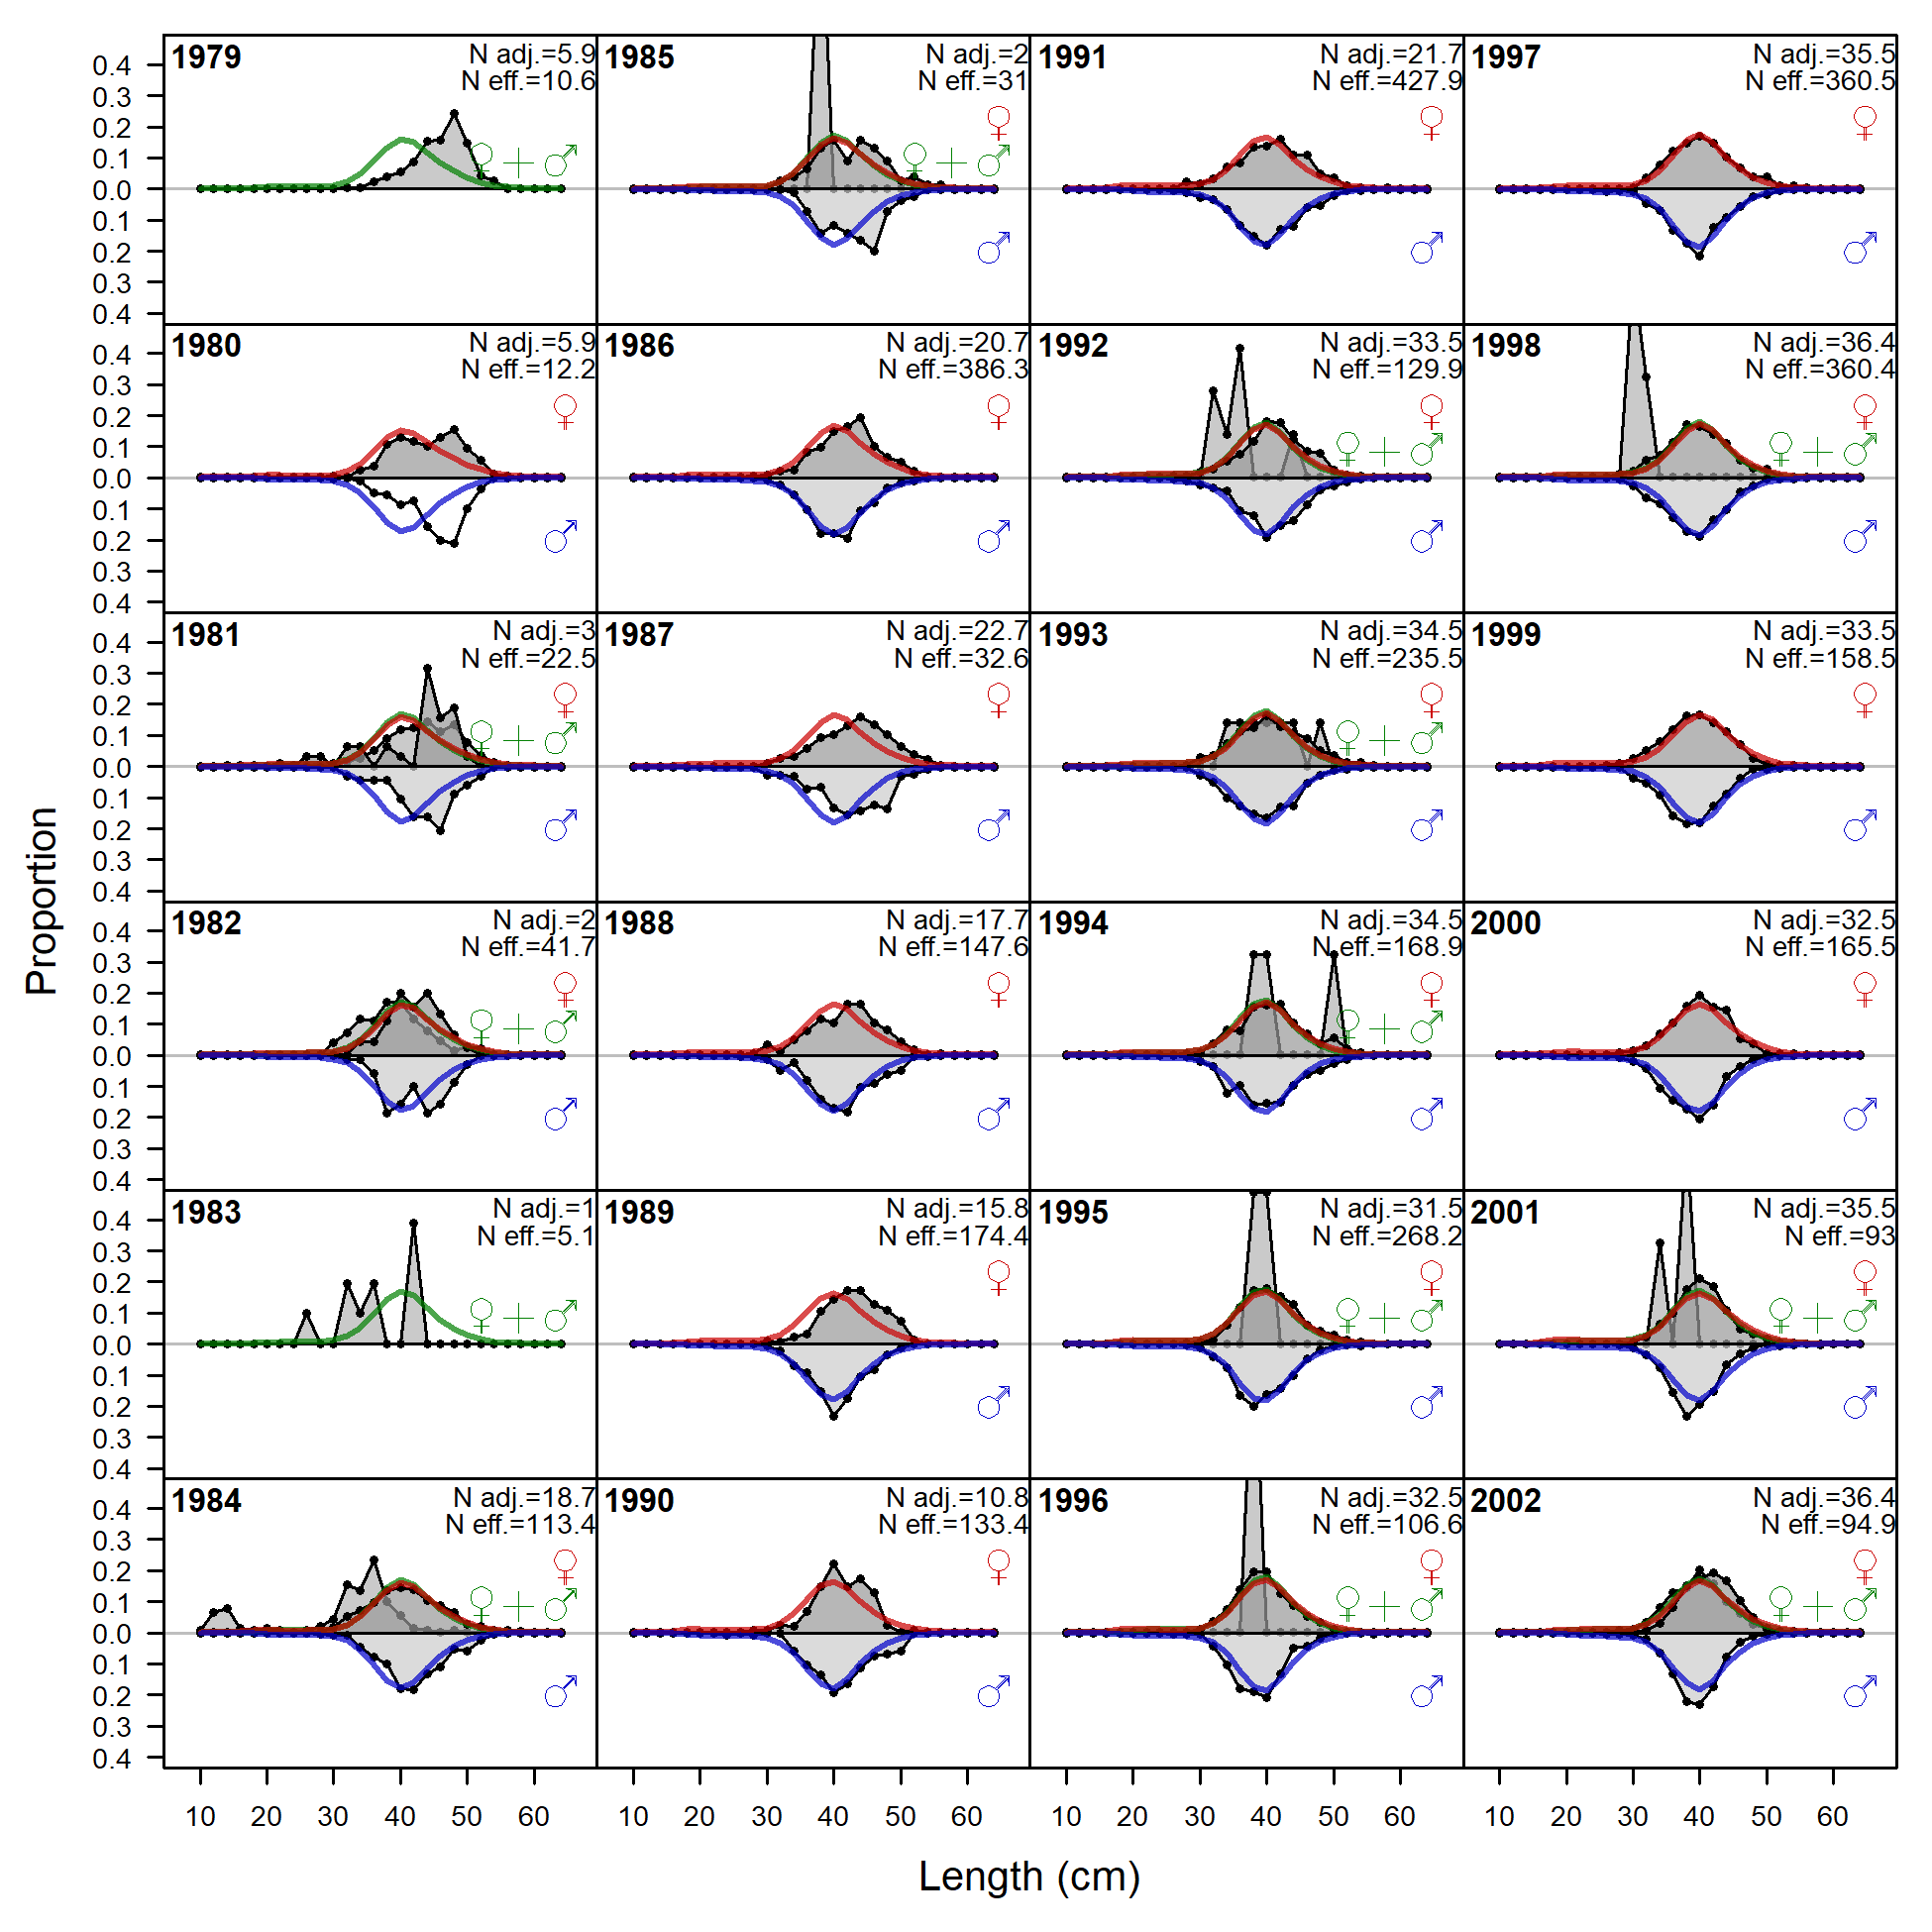
\includegraphics[width=1\textwidth,height=1\textheight]{C:/Users/Jason.Cope/Documents/Github/Sebastes_melanops_WA/Document/models/Reference model/plots/comp_lenfit_flt3mkt0_page1.png}
\caption{Length comps, whole catch, Recreational (plot 1 of 2).`N adj.' is the input sample size after data-weighting adjustment. N eff. is the calculated effective sample size used in the McAllister-Ianelli tuning method.\label{fig:comp_lenfit_flt3mkt0_page1}}
\end{figure}

\begin{figure}
\centering
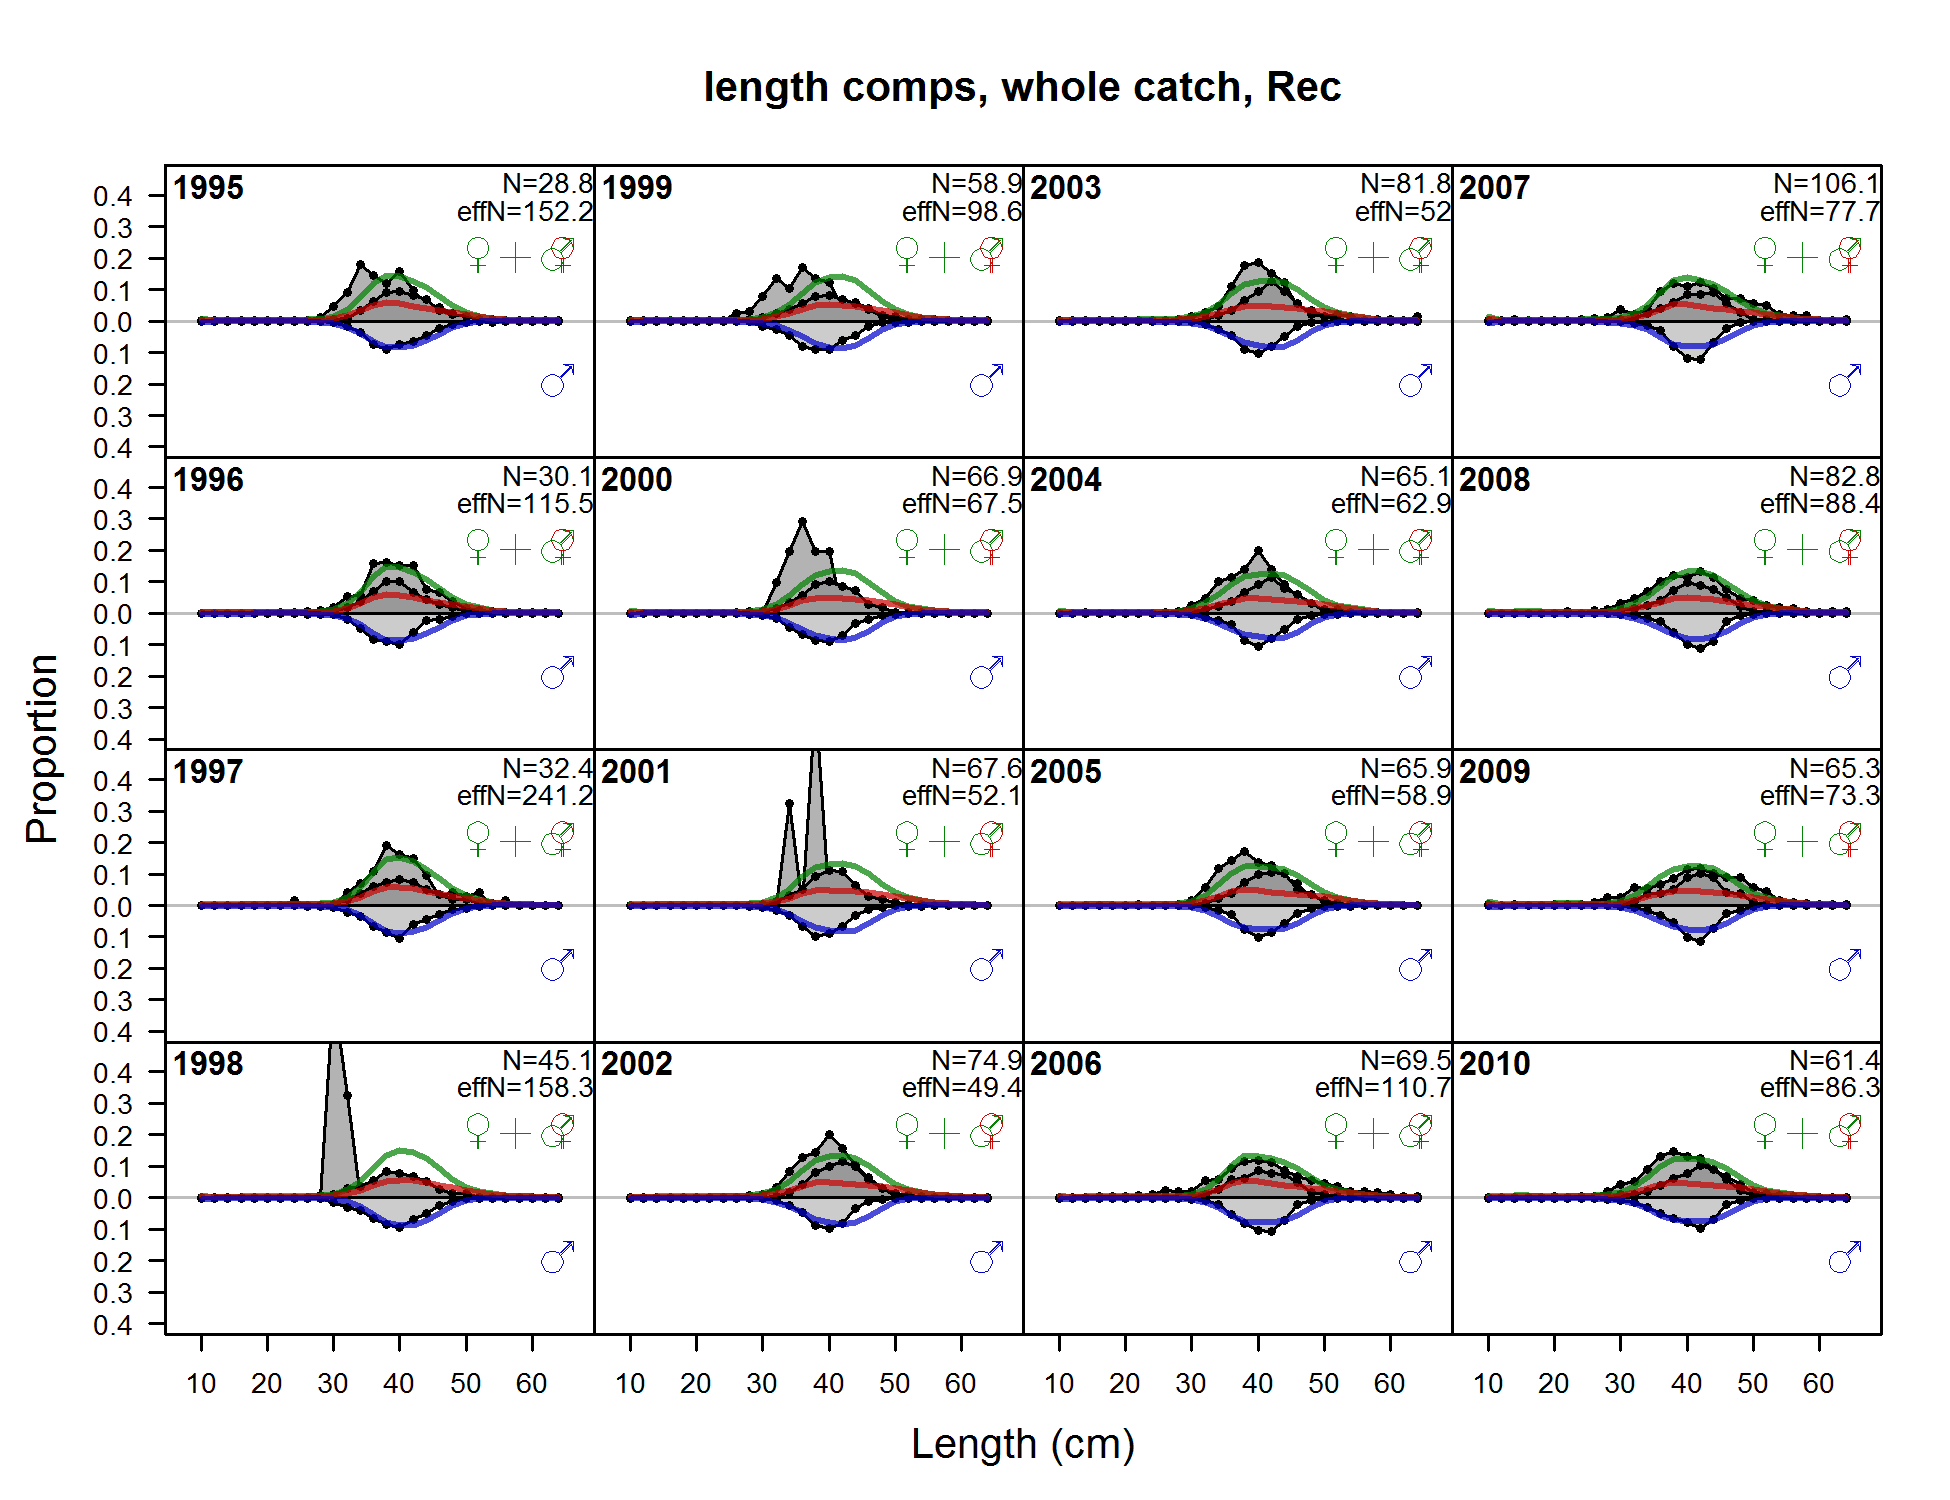
\includegraphics[width=1\textwidth,height=1\textheight]{C:/Users/Jason.Cope/Documents/Github/Sebastes_melanops_WA/Document/models/Reference model/plots/comp_lenfit_flt3mkt0_page2.png}
\caption{Length comps, whole catch, Recreational (plot 1 of 2).`N adj.' is the input sample size after data-weighting adjustment. N eff. is the calculated effective sample size used in the McAllister-Ianelli tuning method. (plot 2 of 2).\label{fig:comp_lenfit_flt3mkt0_page2}}
\end{figure}

\begin{figure}
\centering
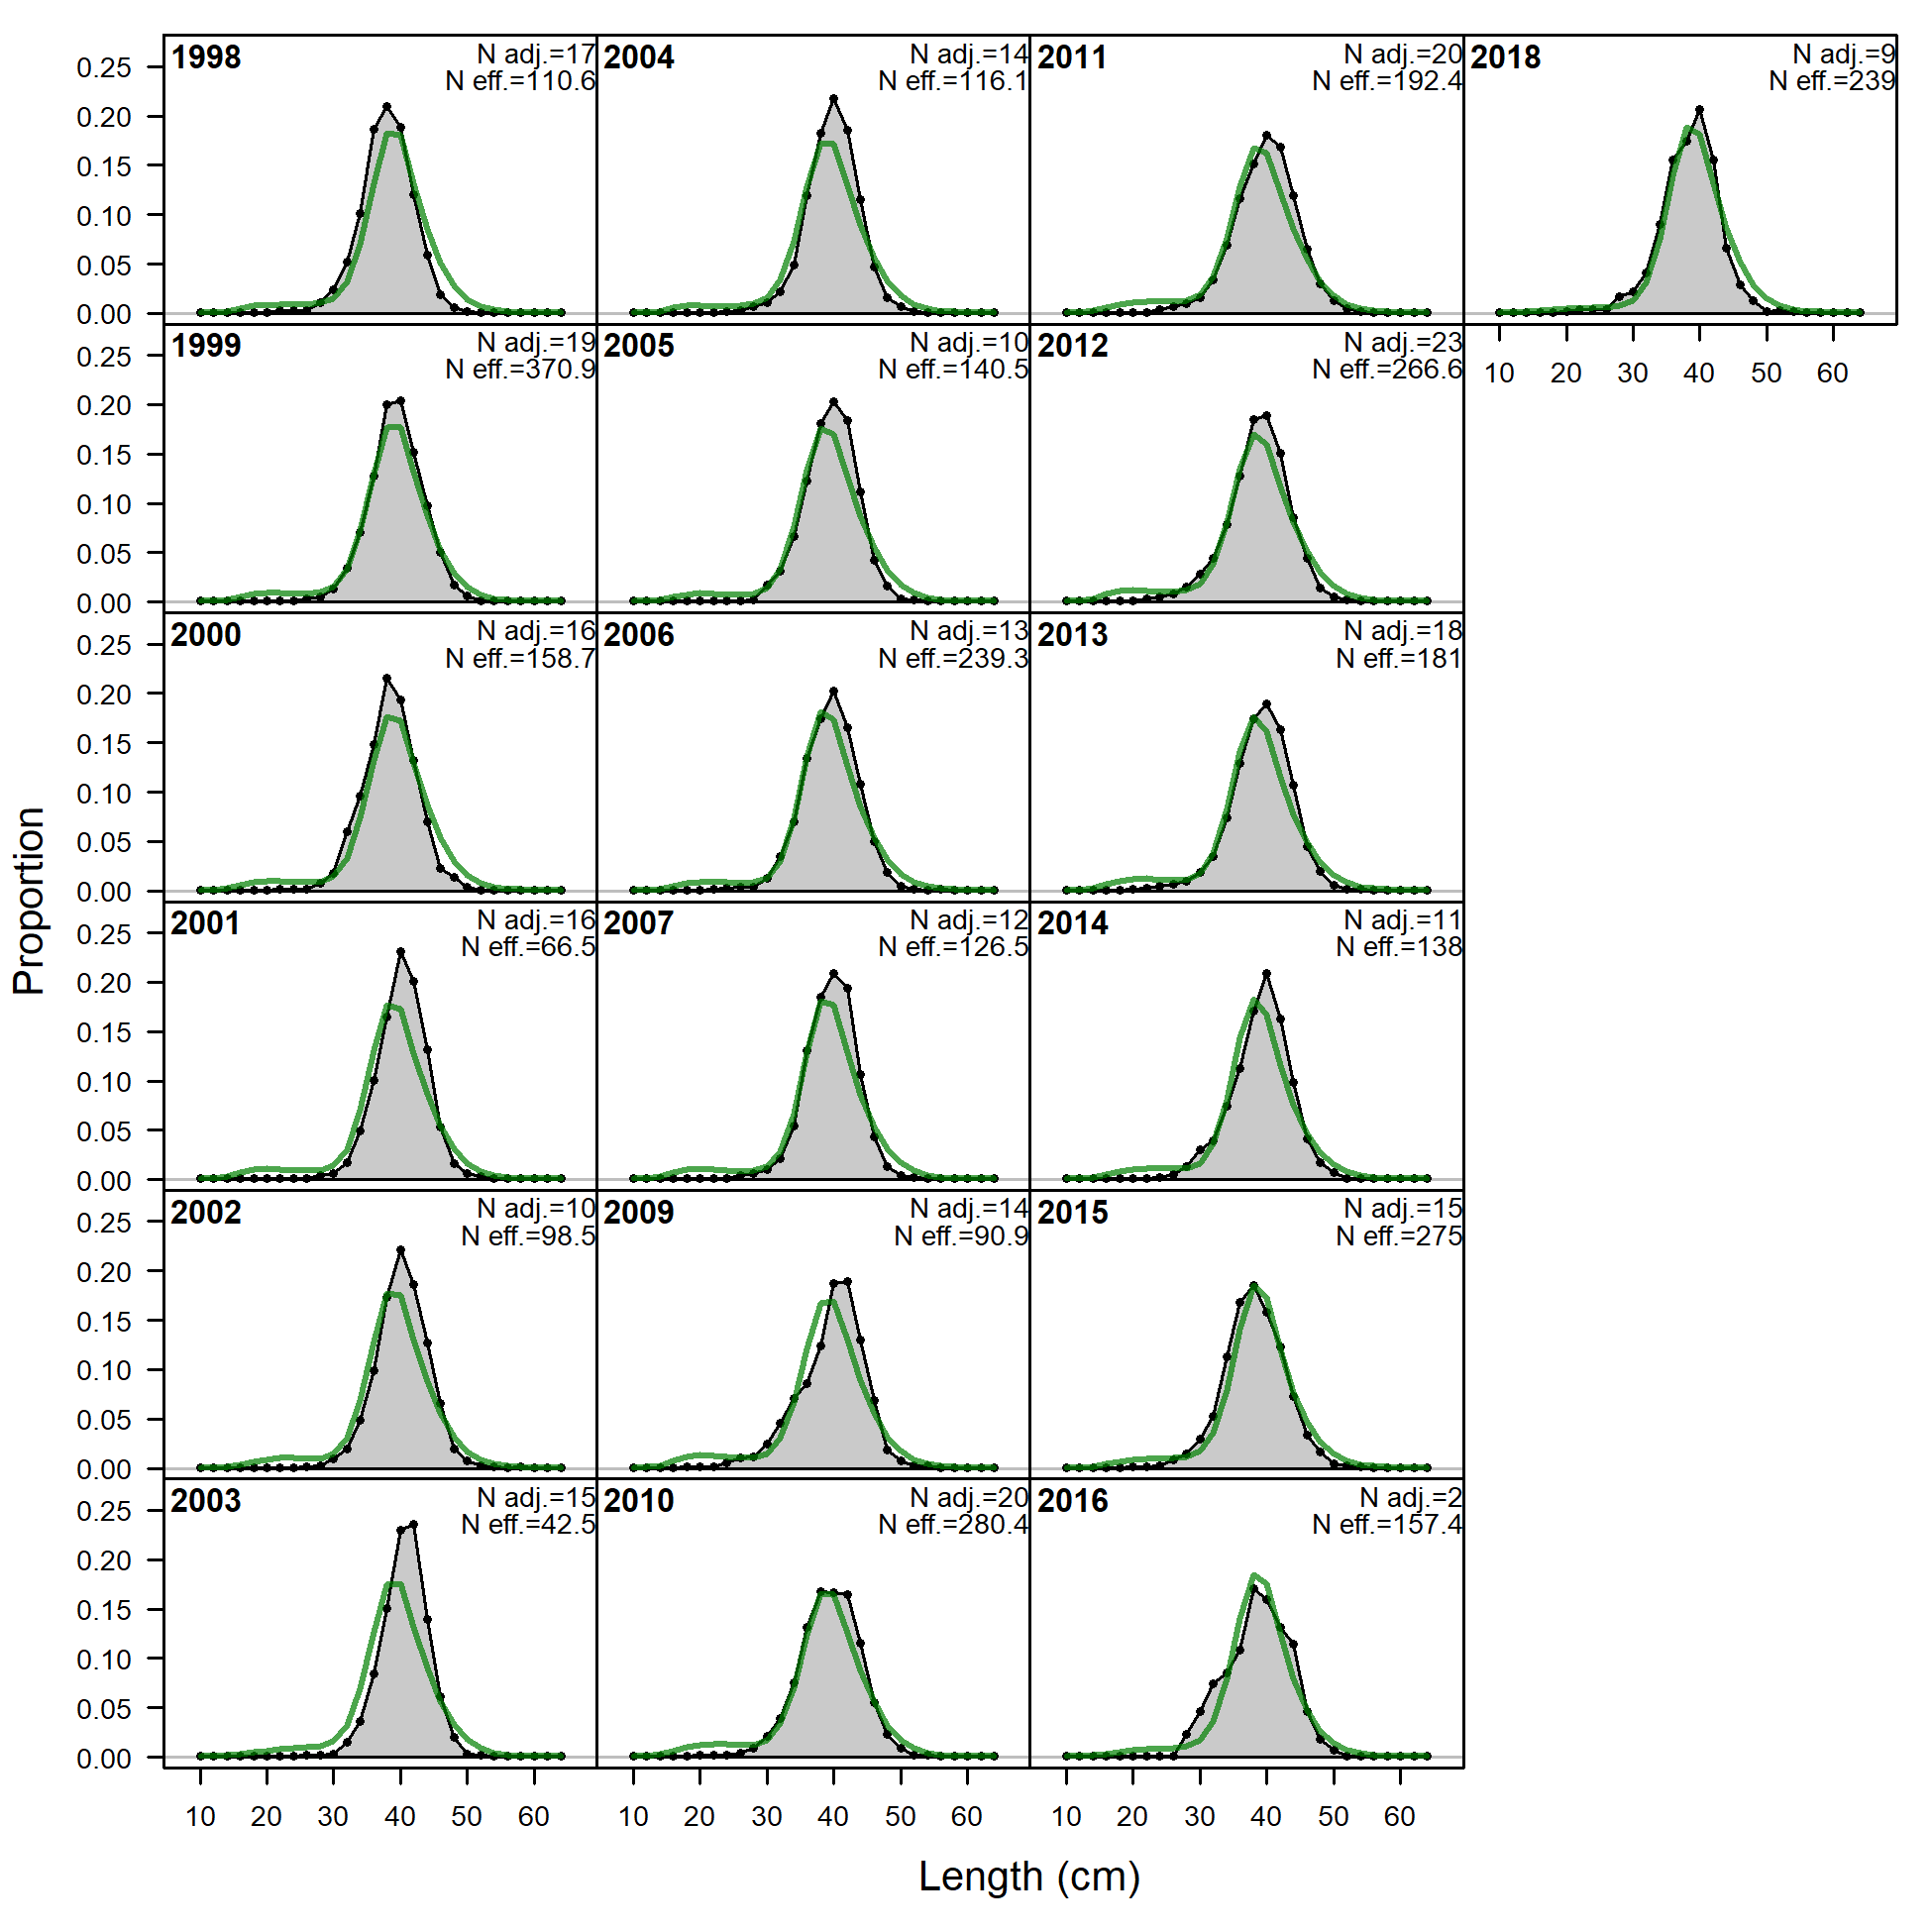
\includegraphics[width=1\textwidth,height=1\textheight]{C:/Users/Jason.Cope/Documents/Github/Sebastes_melanops_WA/Document/models/Reference model/plots/comp_lenfit_flt4mkt0.png}
\caption{Length comps, whole catch, Tagging.`N adj.' is the input sample size after data-weighting adjustment. N eff. is the calculated effective sample size used in the McAllister-Ianelli tuning method.\label{fig:comp_lenfit_flt4mkt0}}
\end{figure}

\begin{figure}
\centering
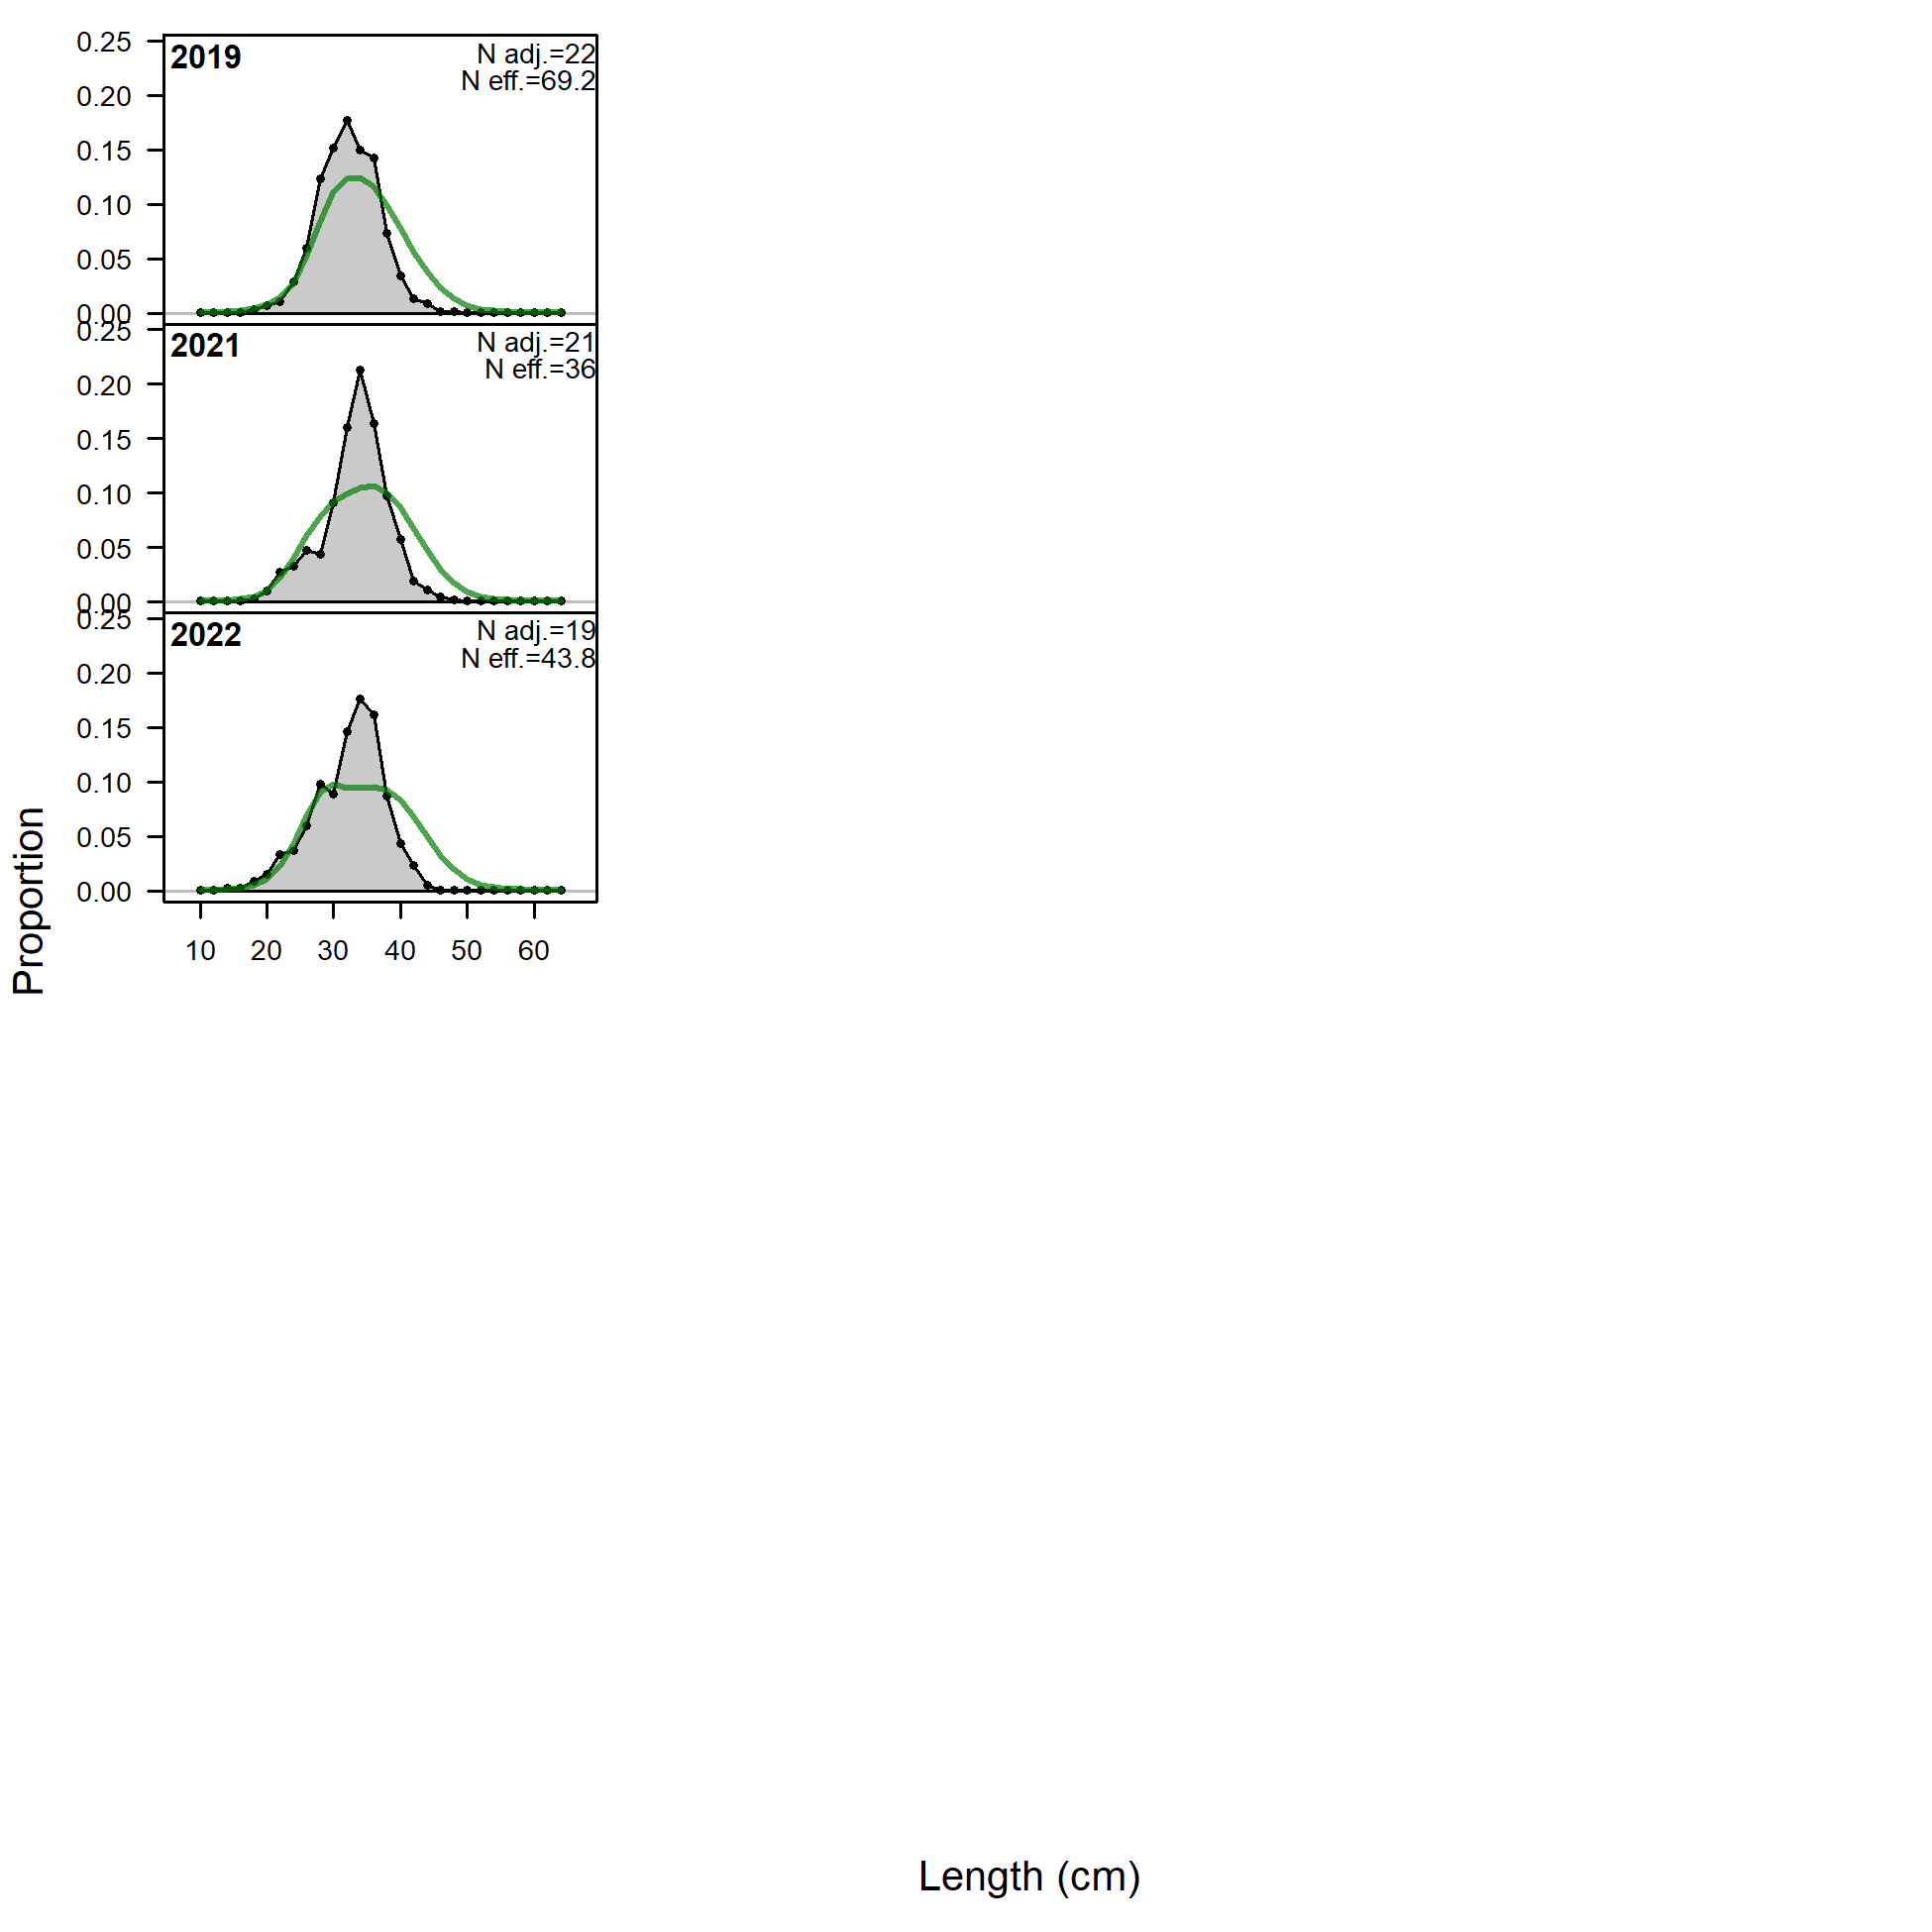
\includegraphics[width=1\textwidth,height=1\textheight]{C:/Users/Jason.Cope/Documents/Github/Sebastes_melanops_WA/Document/models/Reference model/plots/comp_lenfit_flt5mkt0.png}
\caption{Length comps, whole catch, Nearshore\_survey.`N adj.' is the input sample size after data-weighting adjustment. N eff. is the calculated effective sample size used in the McAllister-Ianelli tuning method.\label{fig:comp_lenfit_flt5mkt0}}
\end{figure}

\begin{figure}
\centering
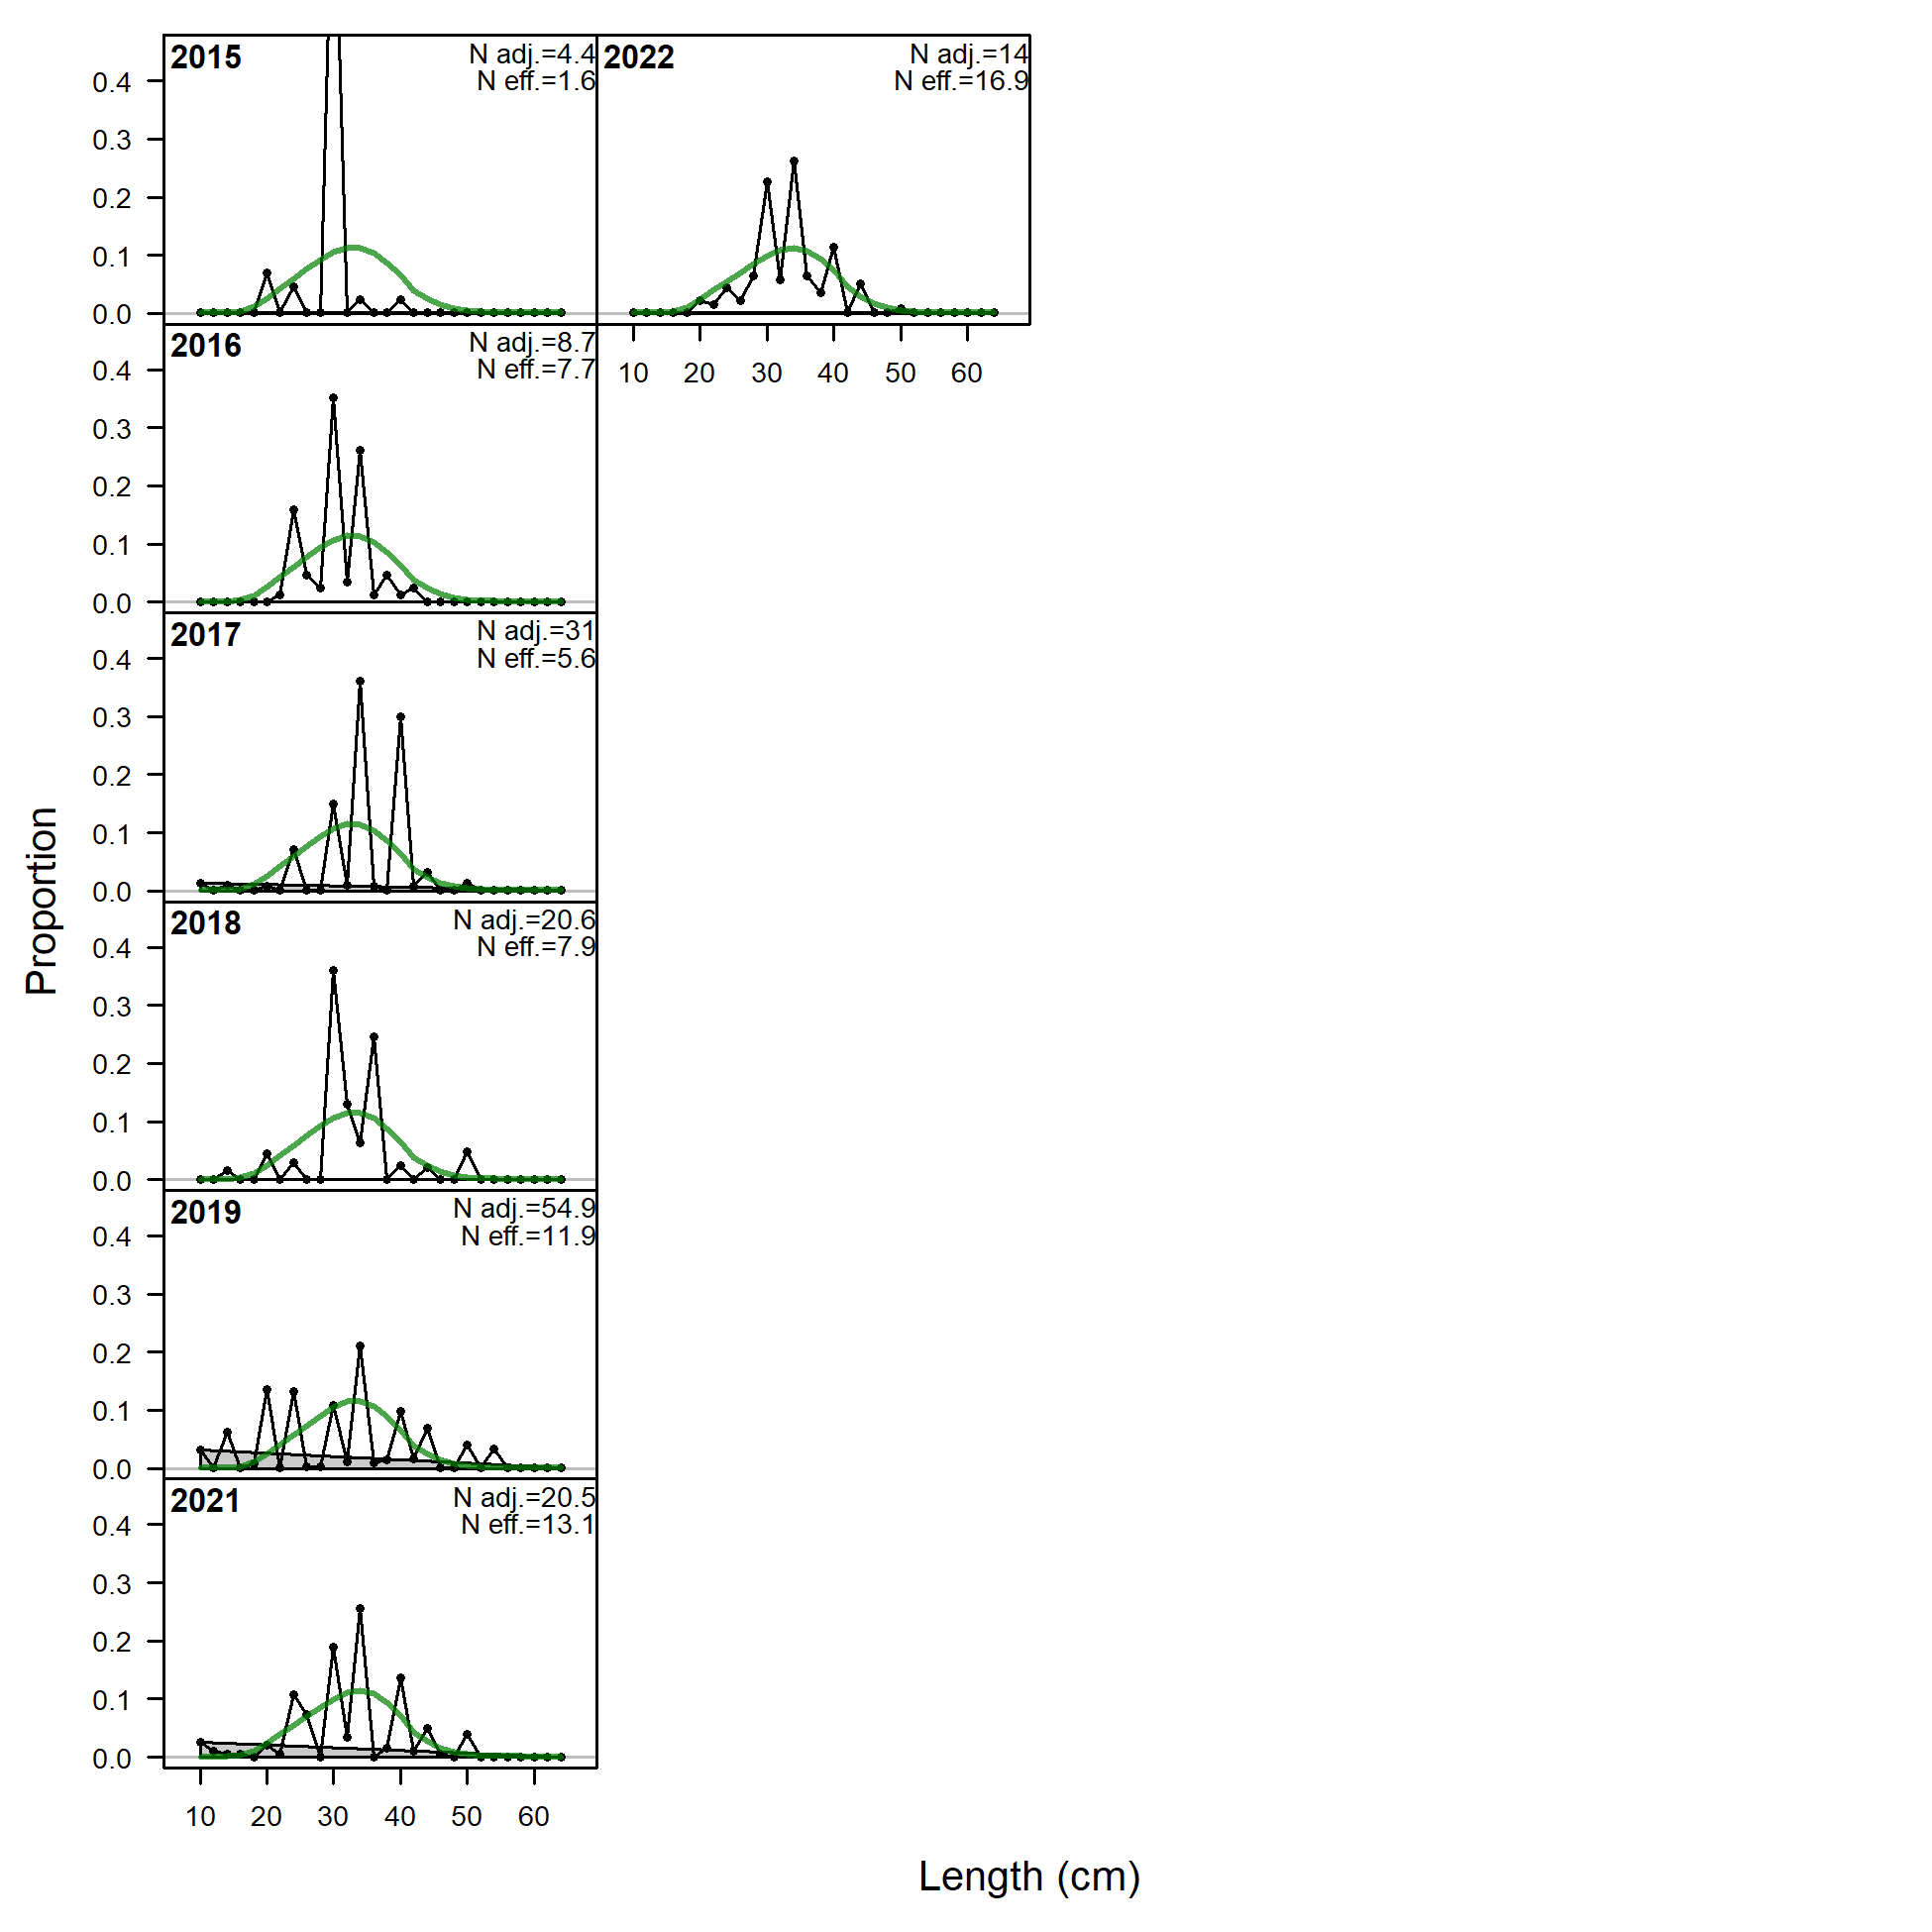
\includegraphics[width=1\textwidth,height=1\textheight]{C:/Users/Jason.Cope/Documents/Github/Sebastes_melanops_WA/Document/models/Reference model/plots/comp_lenfit_flt6mkt0.png}
\caption{Length comps, whole catch, OCNMS.`N adj.' is the input sample size after data-weighting adjustment. N eff. is the calculated effective sample size used in the McAllister-Ianelli tuning method.\label{fig:comp_lenfit_flt6mkt0}}
\end{figure}

\clearpage

\hypertarget{app-b}{%
\section{Appendix B: Fit to Conditional-Age-at-Length Composition Data}\label{app-b}}

\begin{figure}
\centering
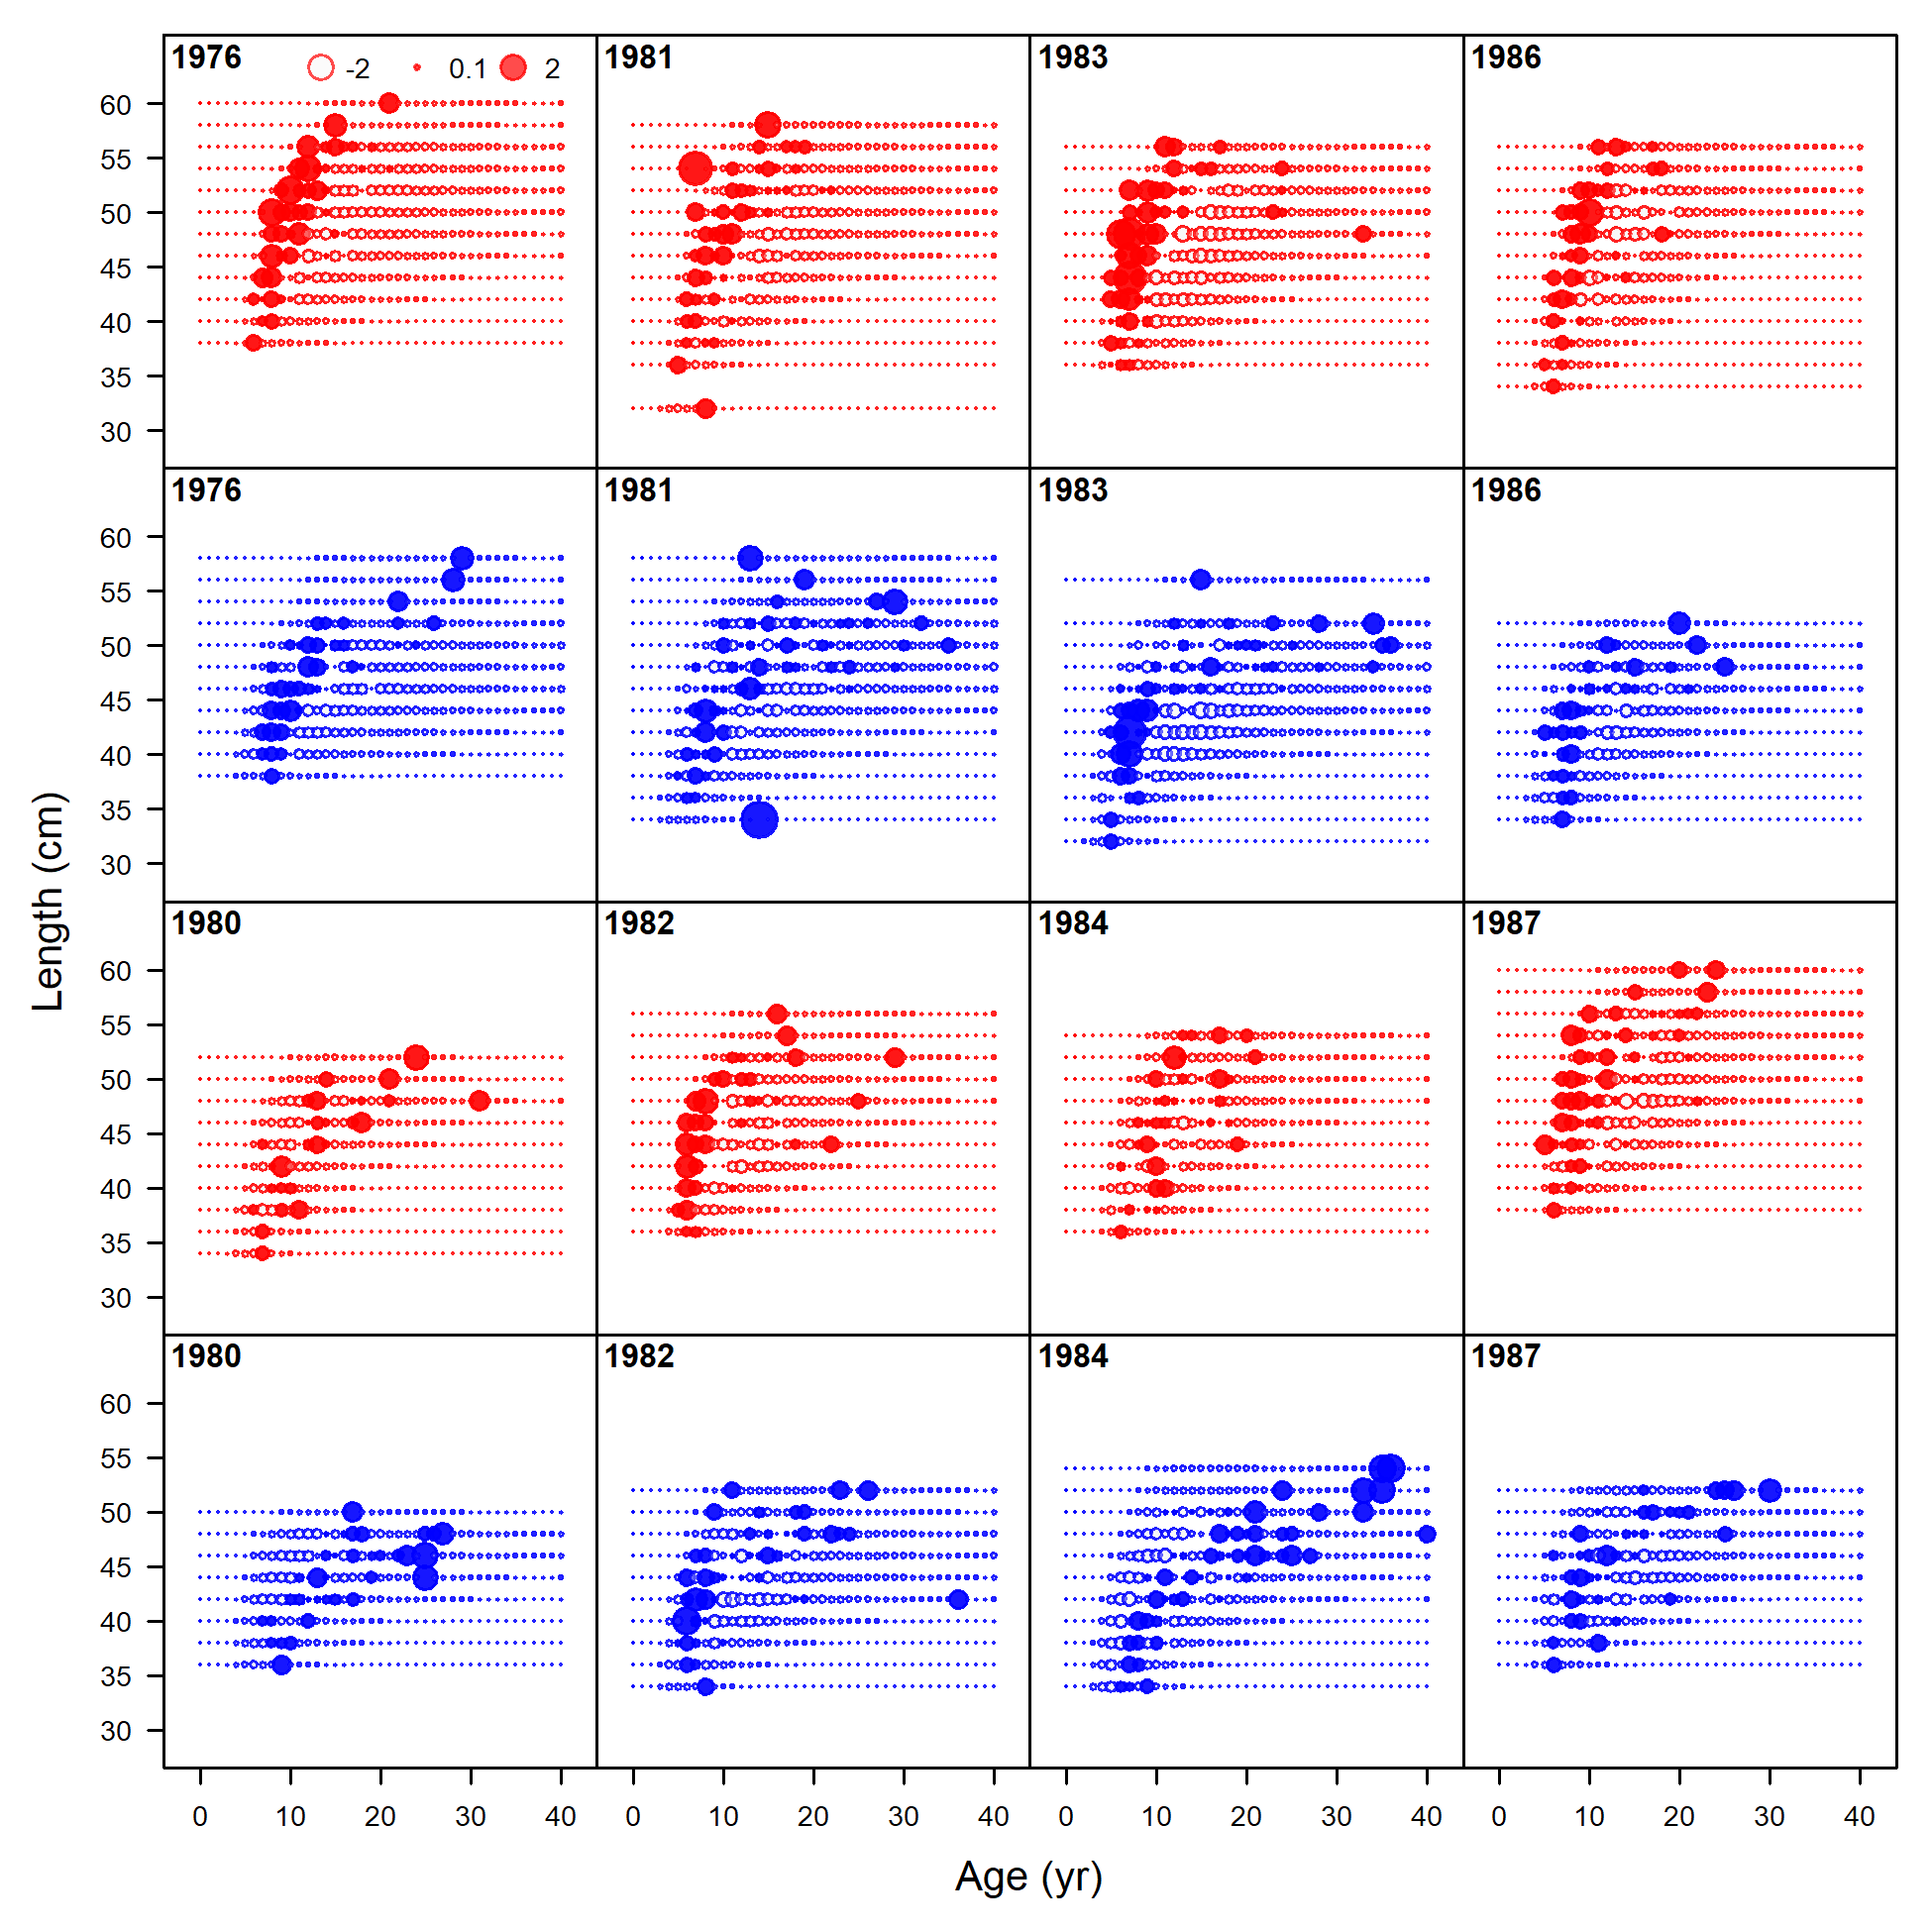
\includegraphics[width=1\textwidth,height=1\textheight]{C:/Users/Jason.Cope/Documents/Github/Sebastes_melanops_WA/Document/models/Reference model/plots/comp_condAALfit_residsflt1mkt0_page1.png}
\caption{Pearson residuals, whole catch, Trawl (max=8.71) (plot 1 of 3).\label{fig:comp_condAALfit_residsflt1mkt0_page1}}
\end{figure}

\begin{figure}
\centering
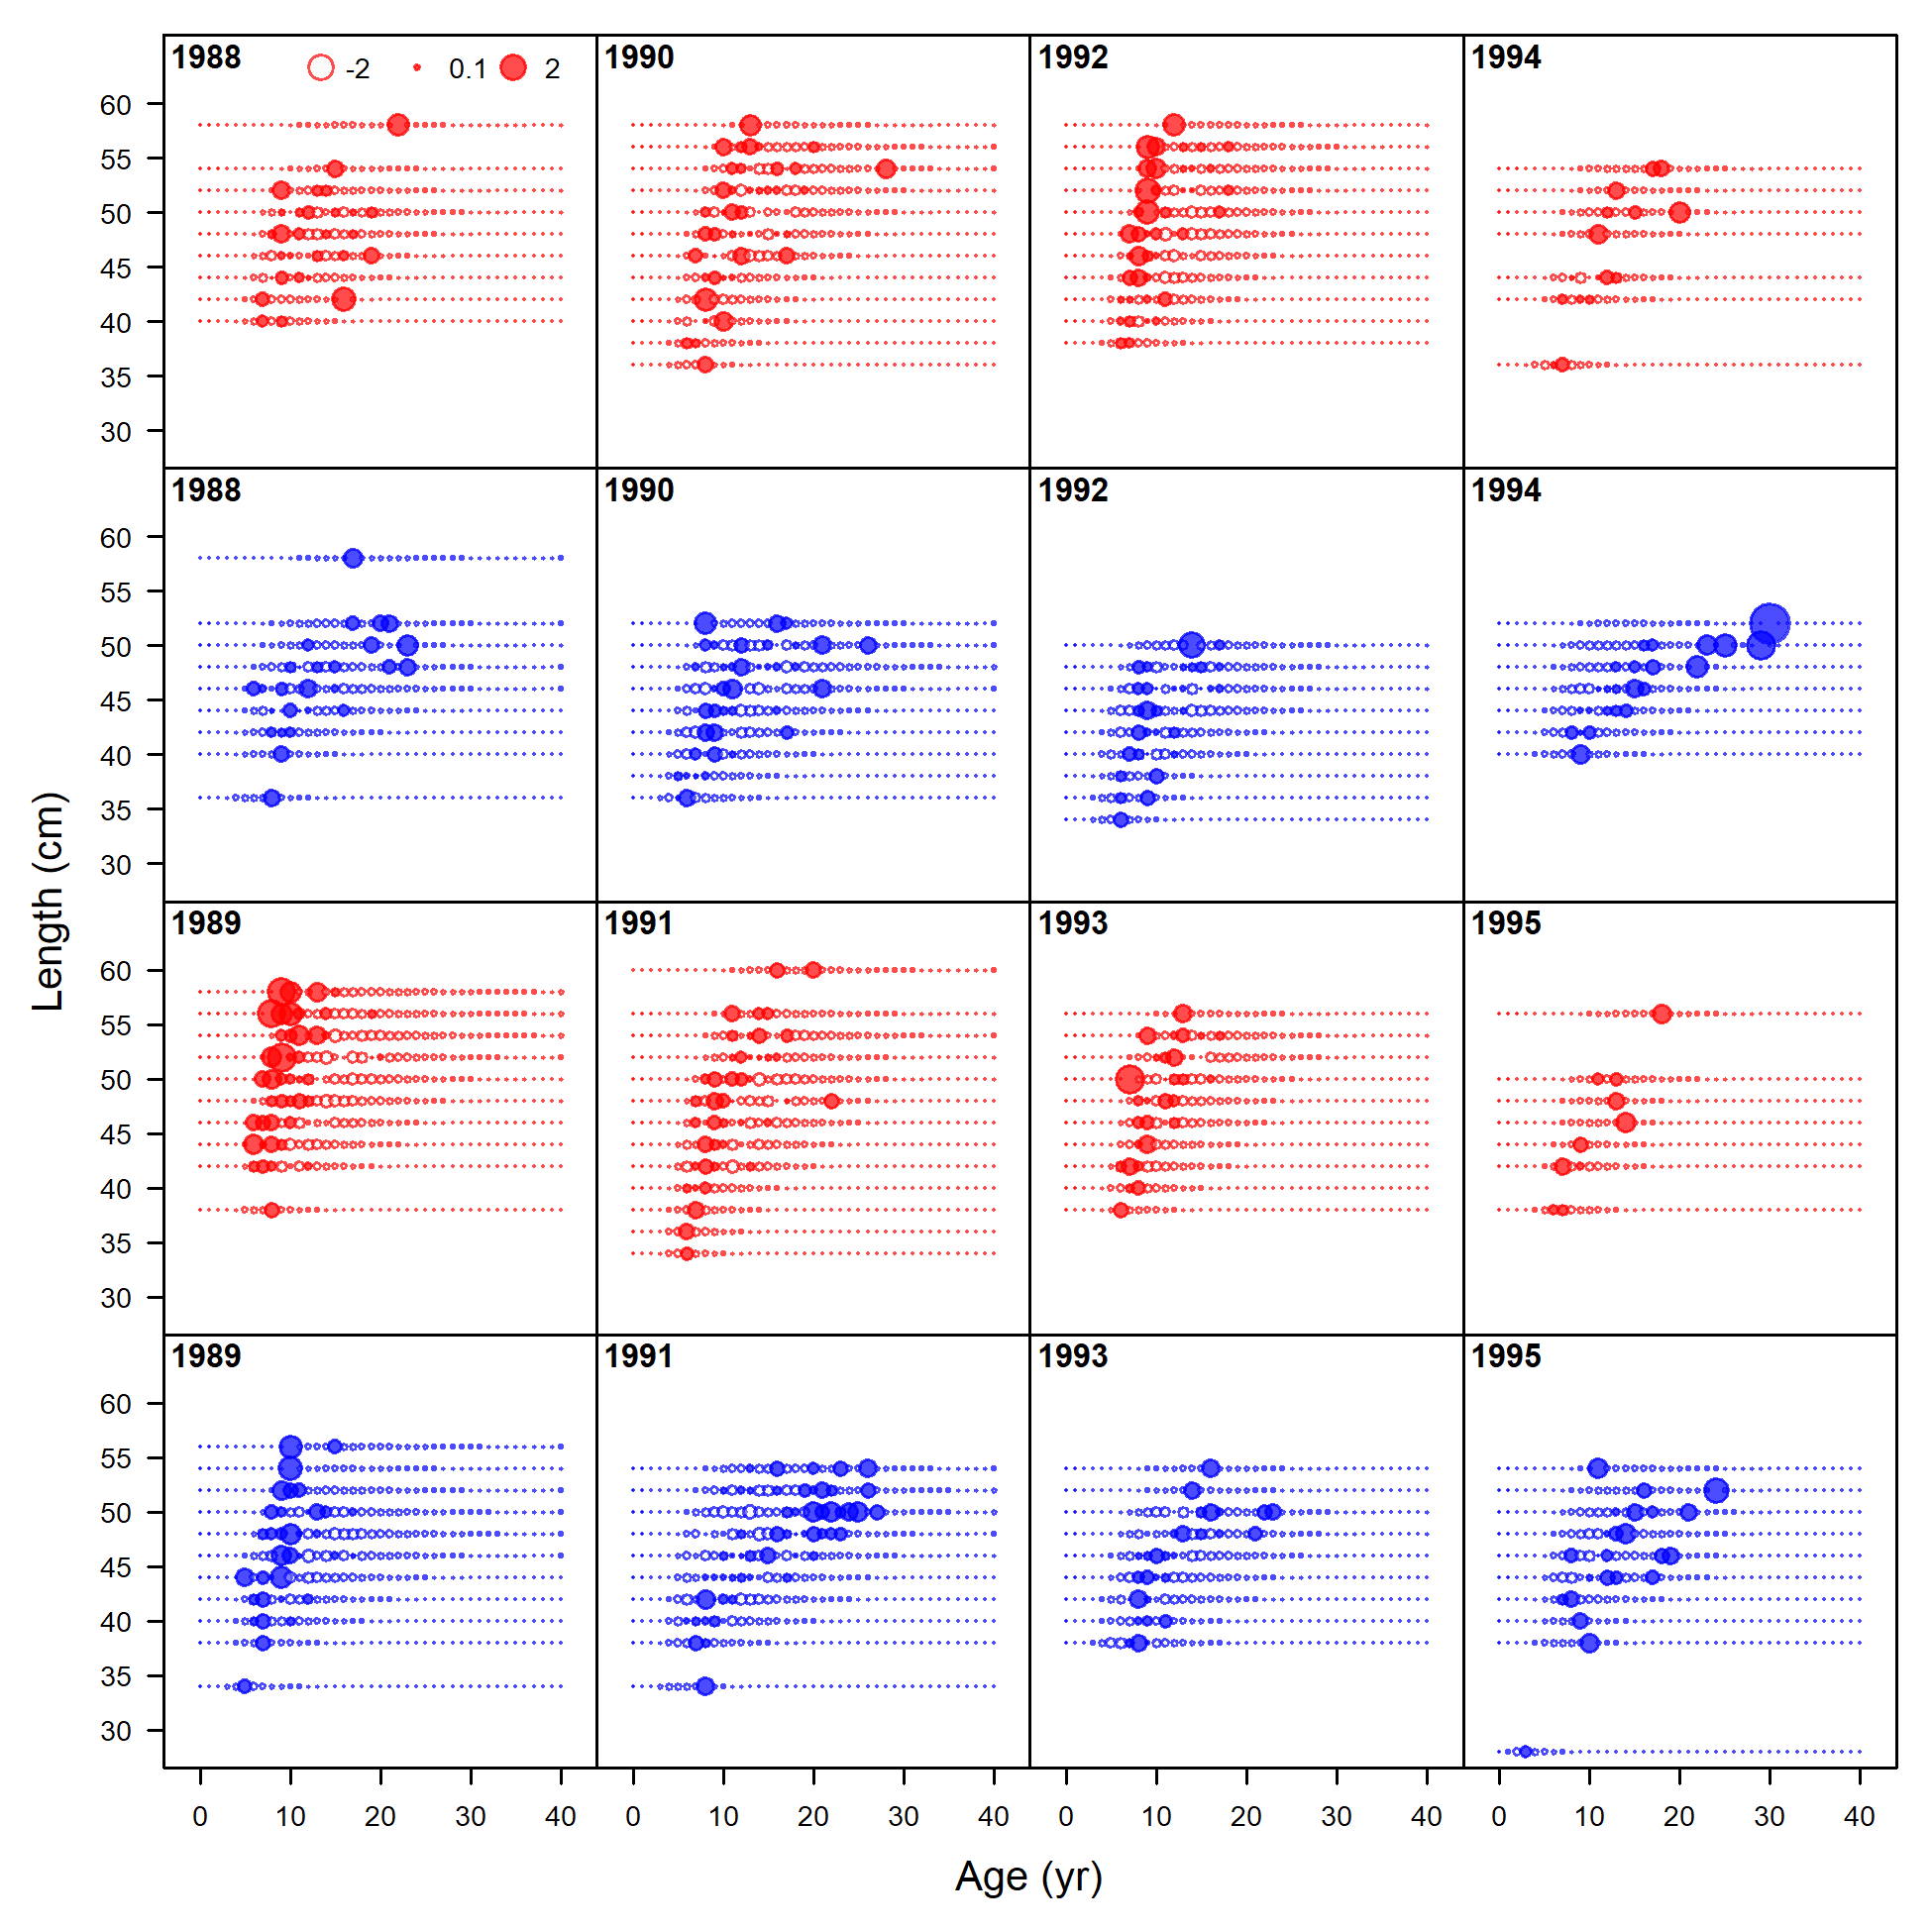
\includegraphics[width=1\textwidth,height=1\textheight]{C:/Users/Jason.Cope/Documents/Github/Sebastes_melanops_WA/Document/models/Reference model/plots/comp_condAALfit_residsflt1mkt0_page2.png}
\caption{Pearson residuals, whole catch, Trawl (max=8.71) (plot 2 of 3).\label{fig:comp_condAALfit_residsflt1mkt0_page2}}
\end{figure}

\begin{figure}
\centering
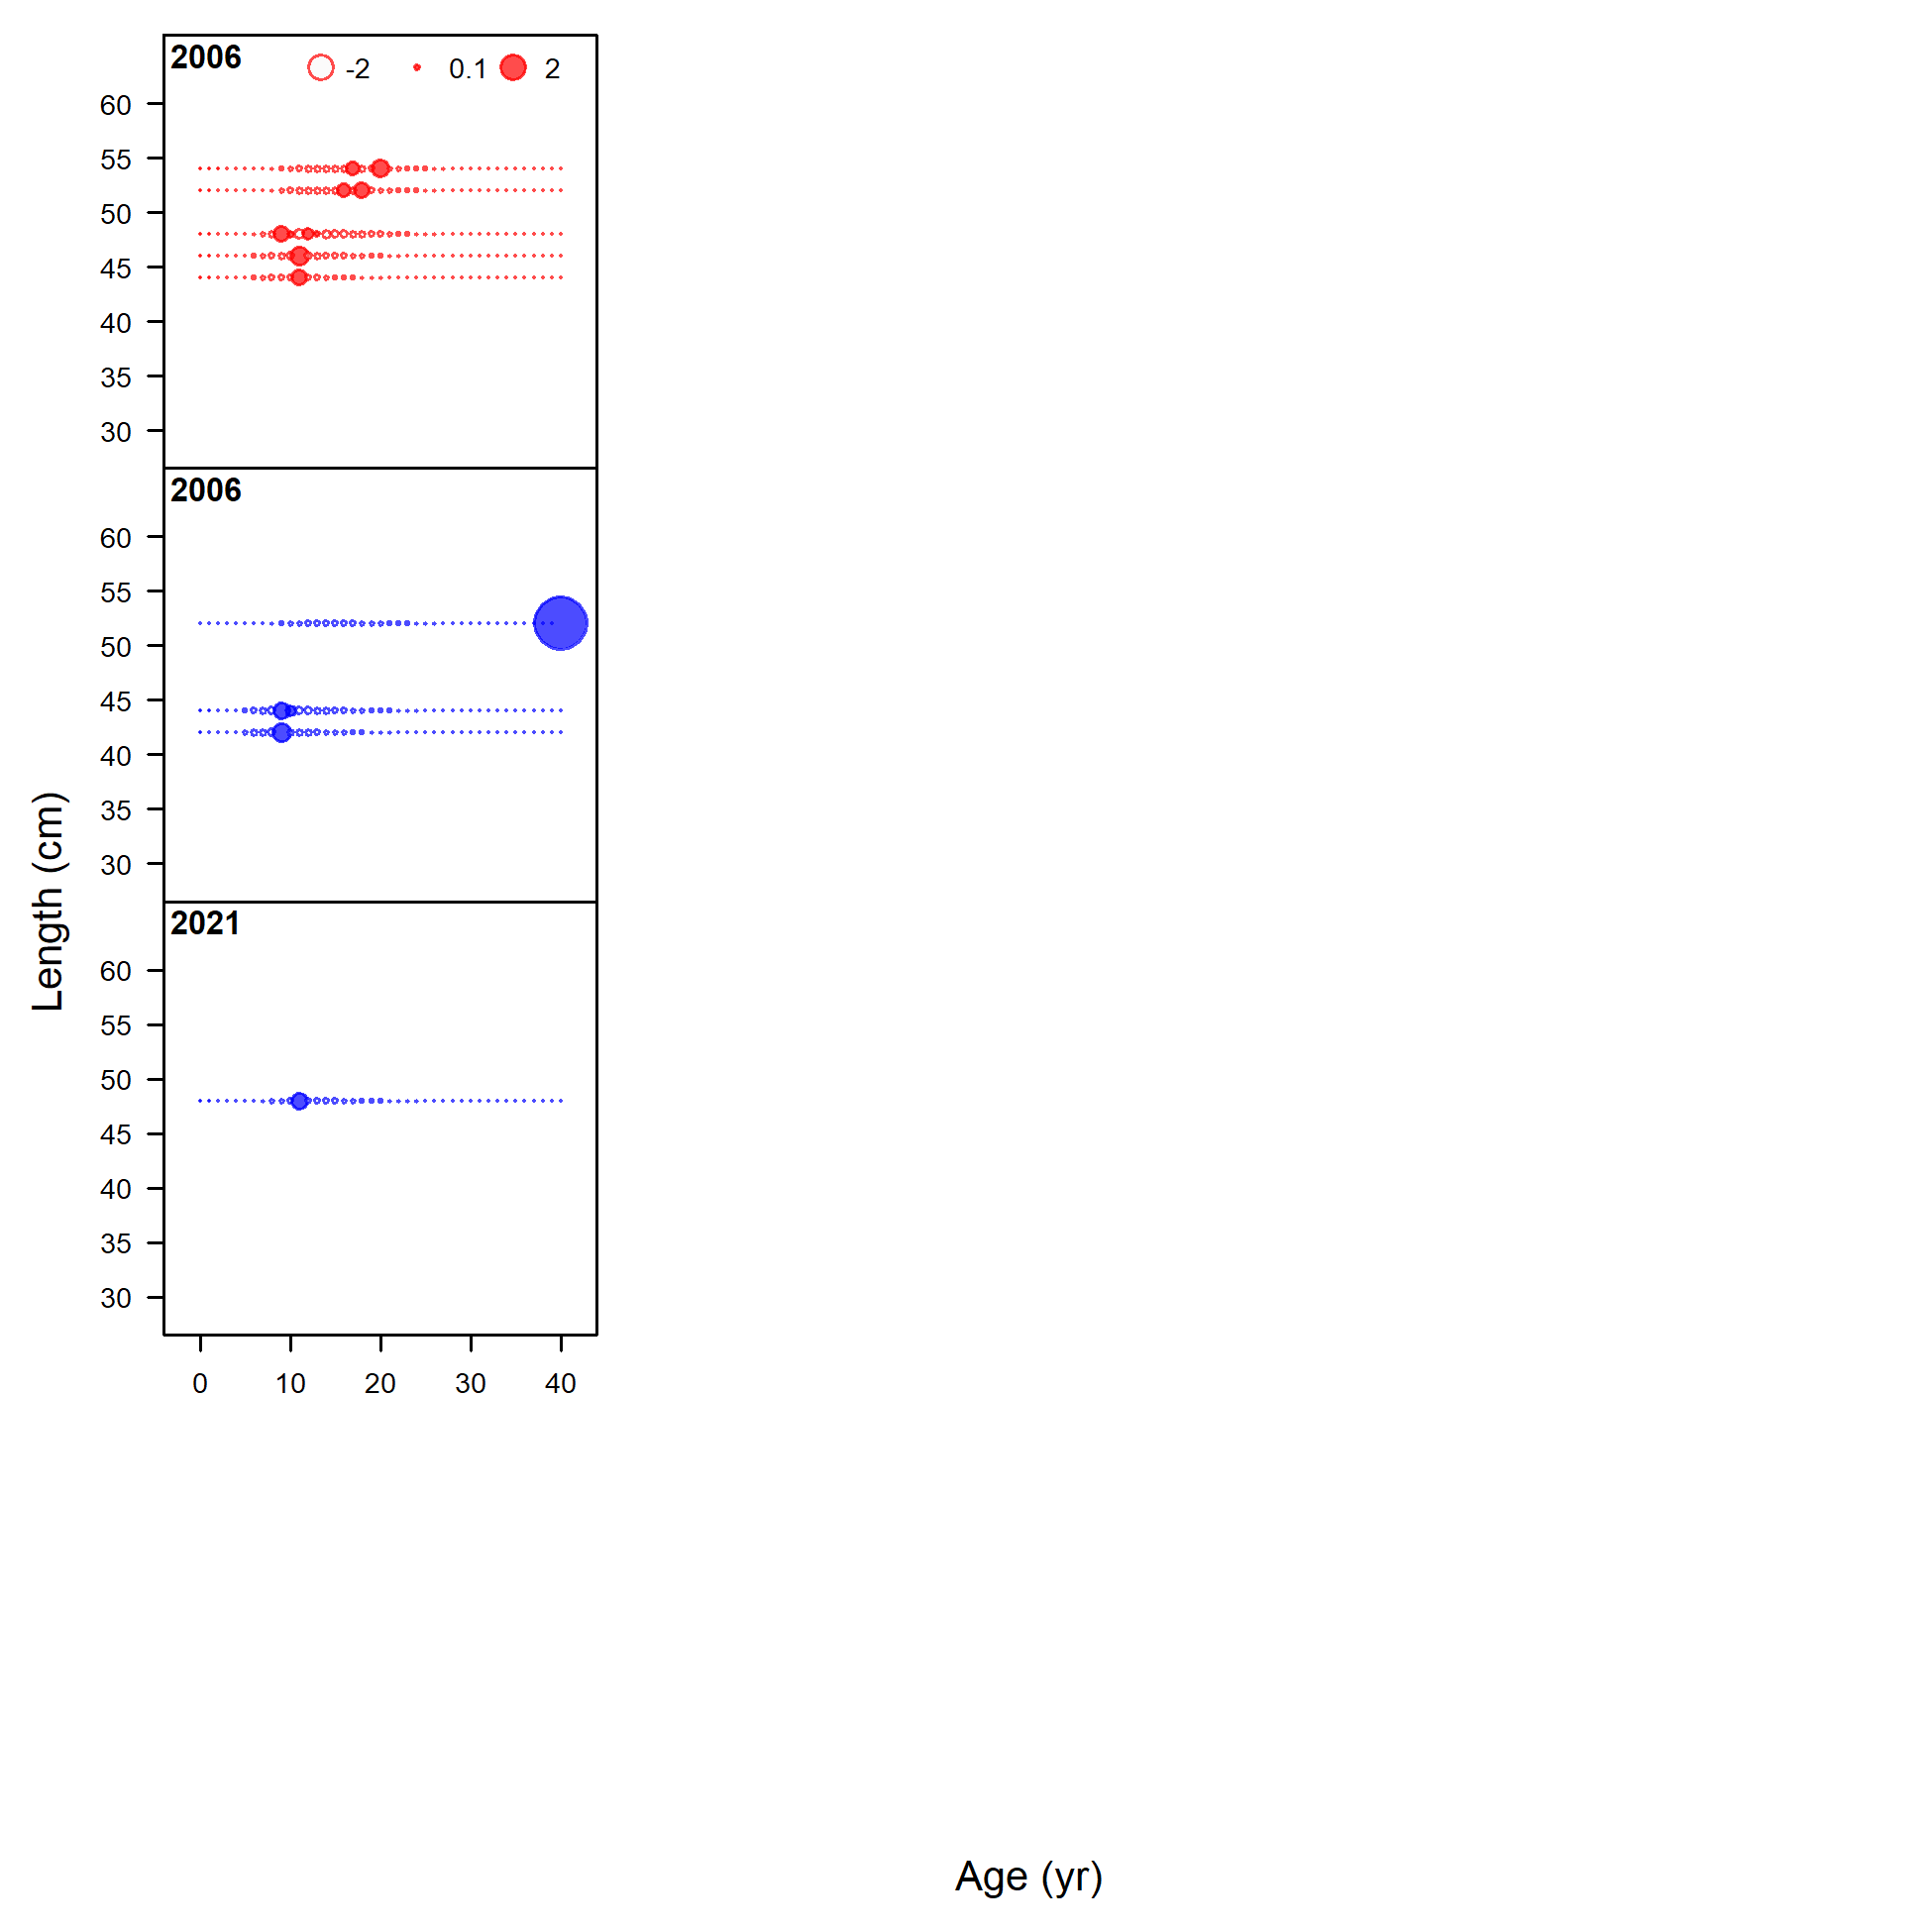
\includegraphics[width=1\textwidth,height=1\textheight]{C:/Users/Jason.Cope/Documents/Github/Sebastes_melanops_WA/Document/models/Reference model/plots/comp_condAALfit_residsflt1mkt0_page3.png}
\caption{Pearson residuals, whole catch, Trawl (max=8.71) (plot 3 of 3).\label{fig:comp_condAALfit_residsflt1mkt0_page3}}
\end{figure}

\begin{figure}
\centering
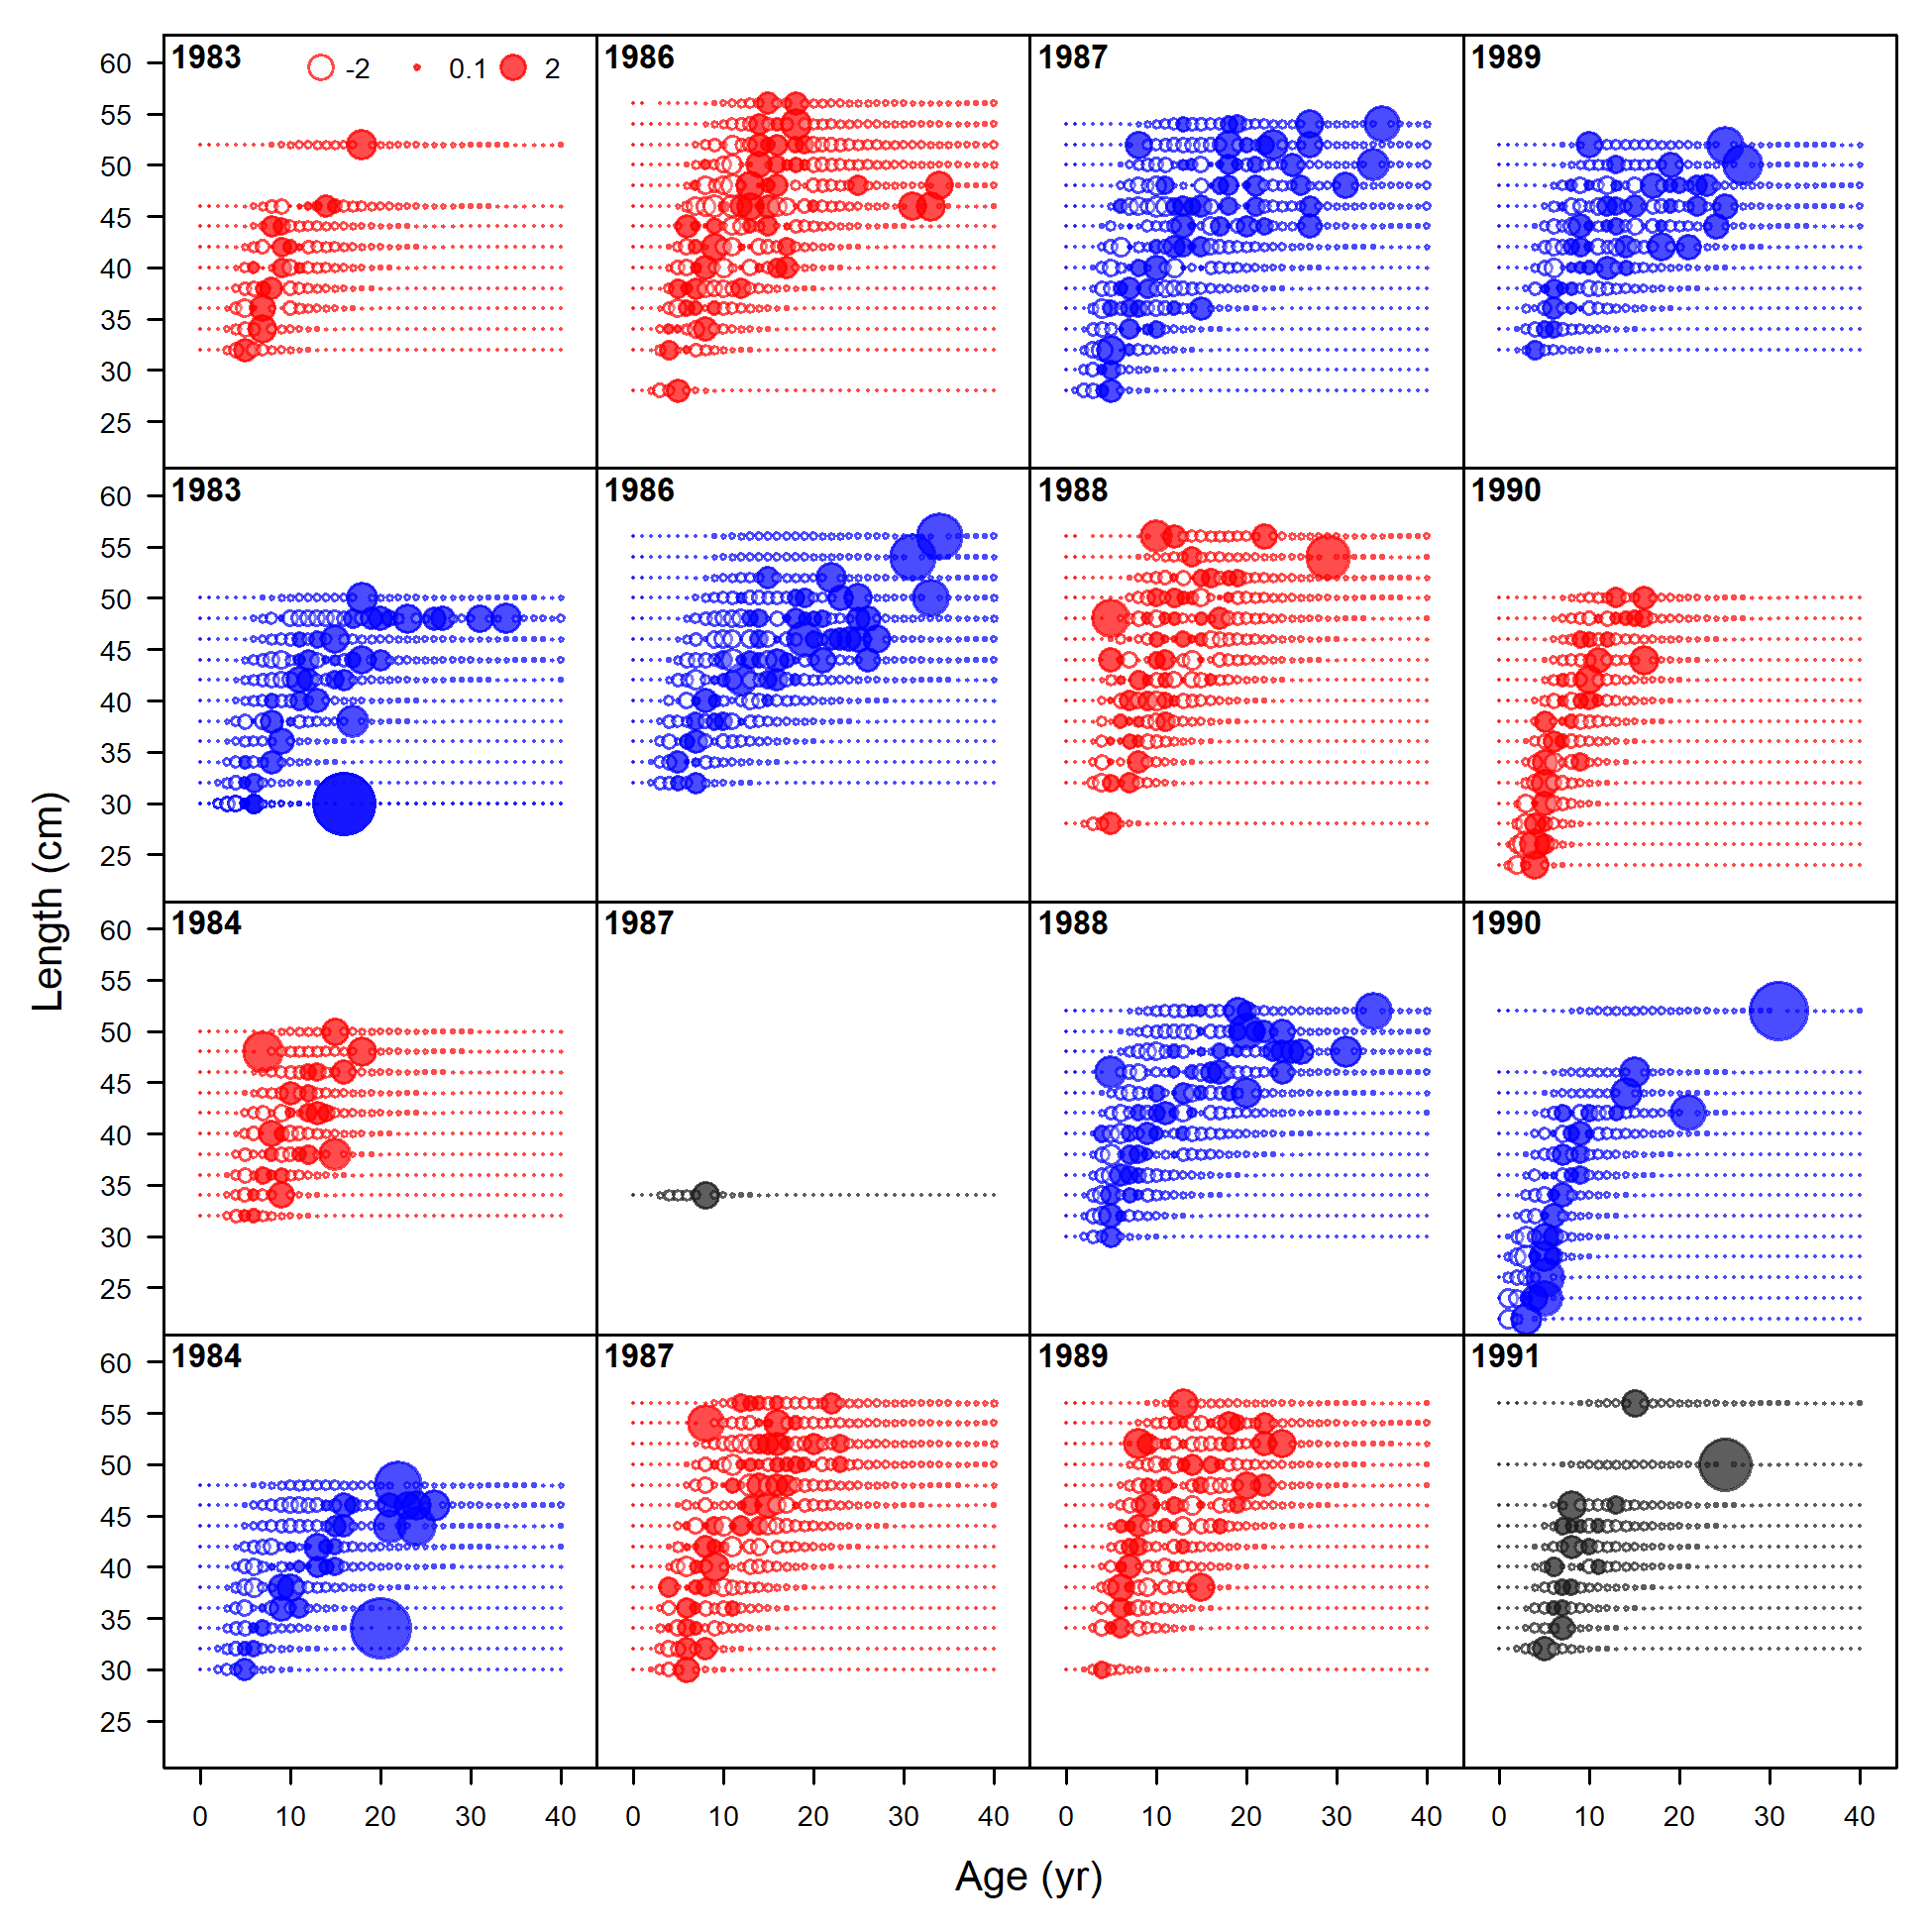
\includegraphics[width=1\textwidth,height=1\textheight]{C:/Users/Jason.Cope/Documents/Github/Sebastes_melanops_WA/Document/models/Reference model/plots/comp_condAALfit_residsflt2mkt0_page1.png}
\caption{Pearson residuals, whole catch, NonTRWL (max=18.54) (plot 1 of 2).\label{fig:comp_condAALfit_residsflt2mkt0_page1}}
\end{figure}

\begin{figure}
\centering
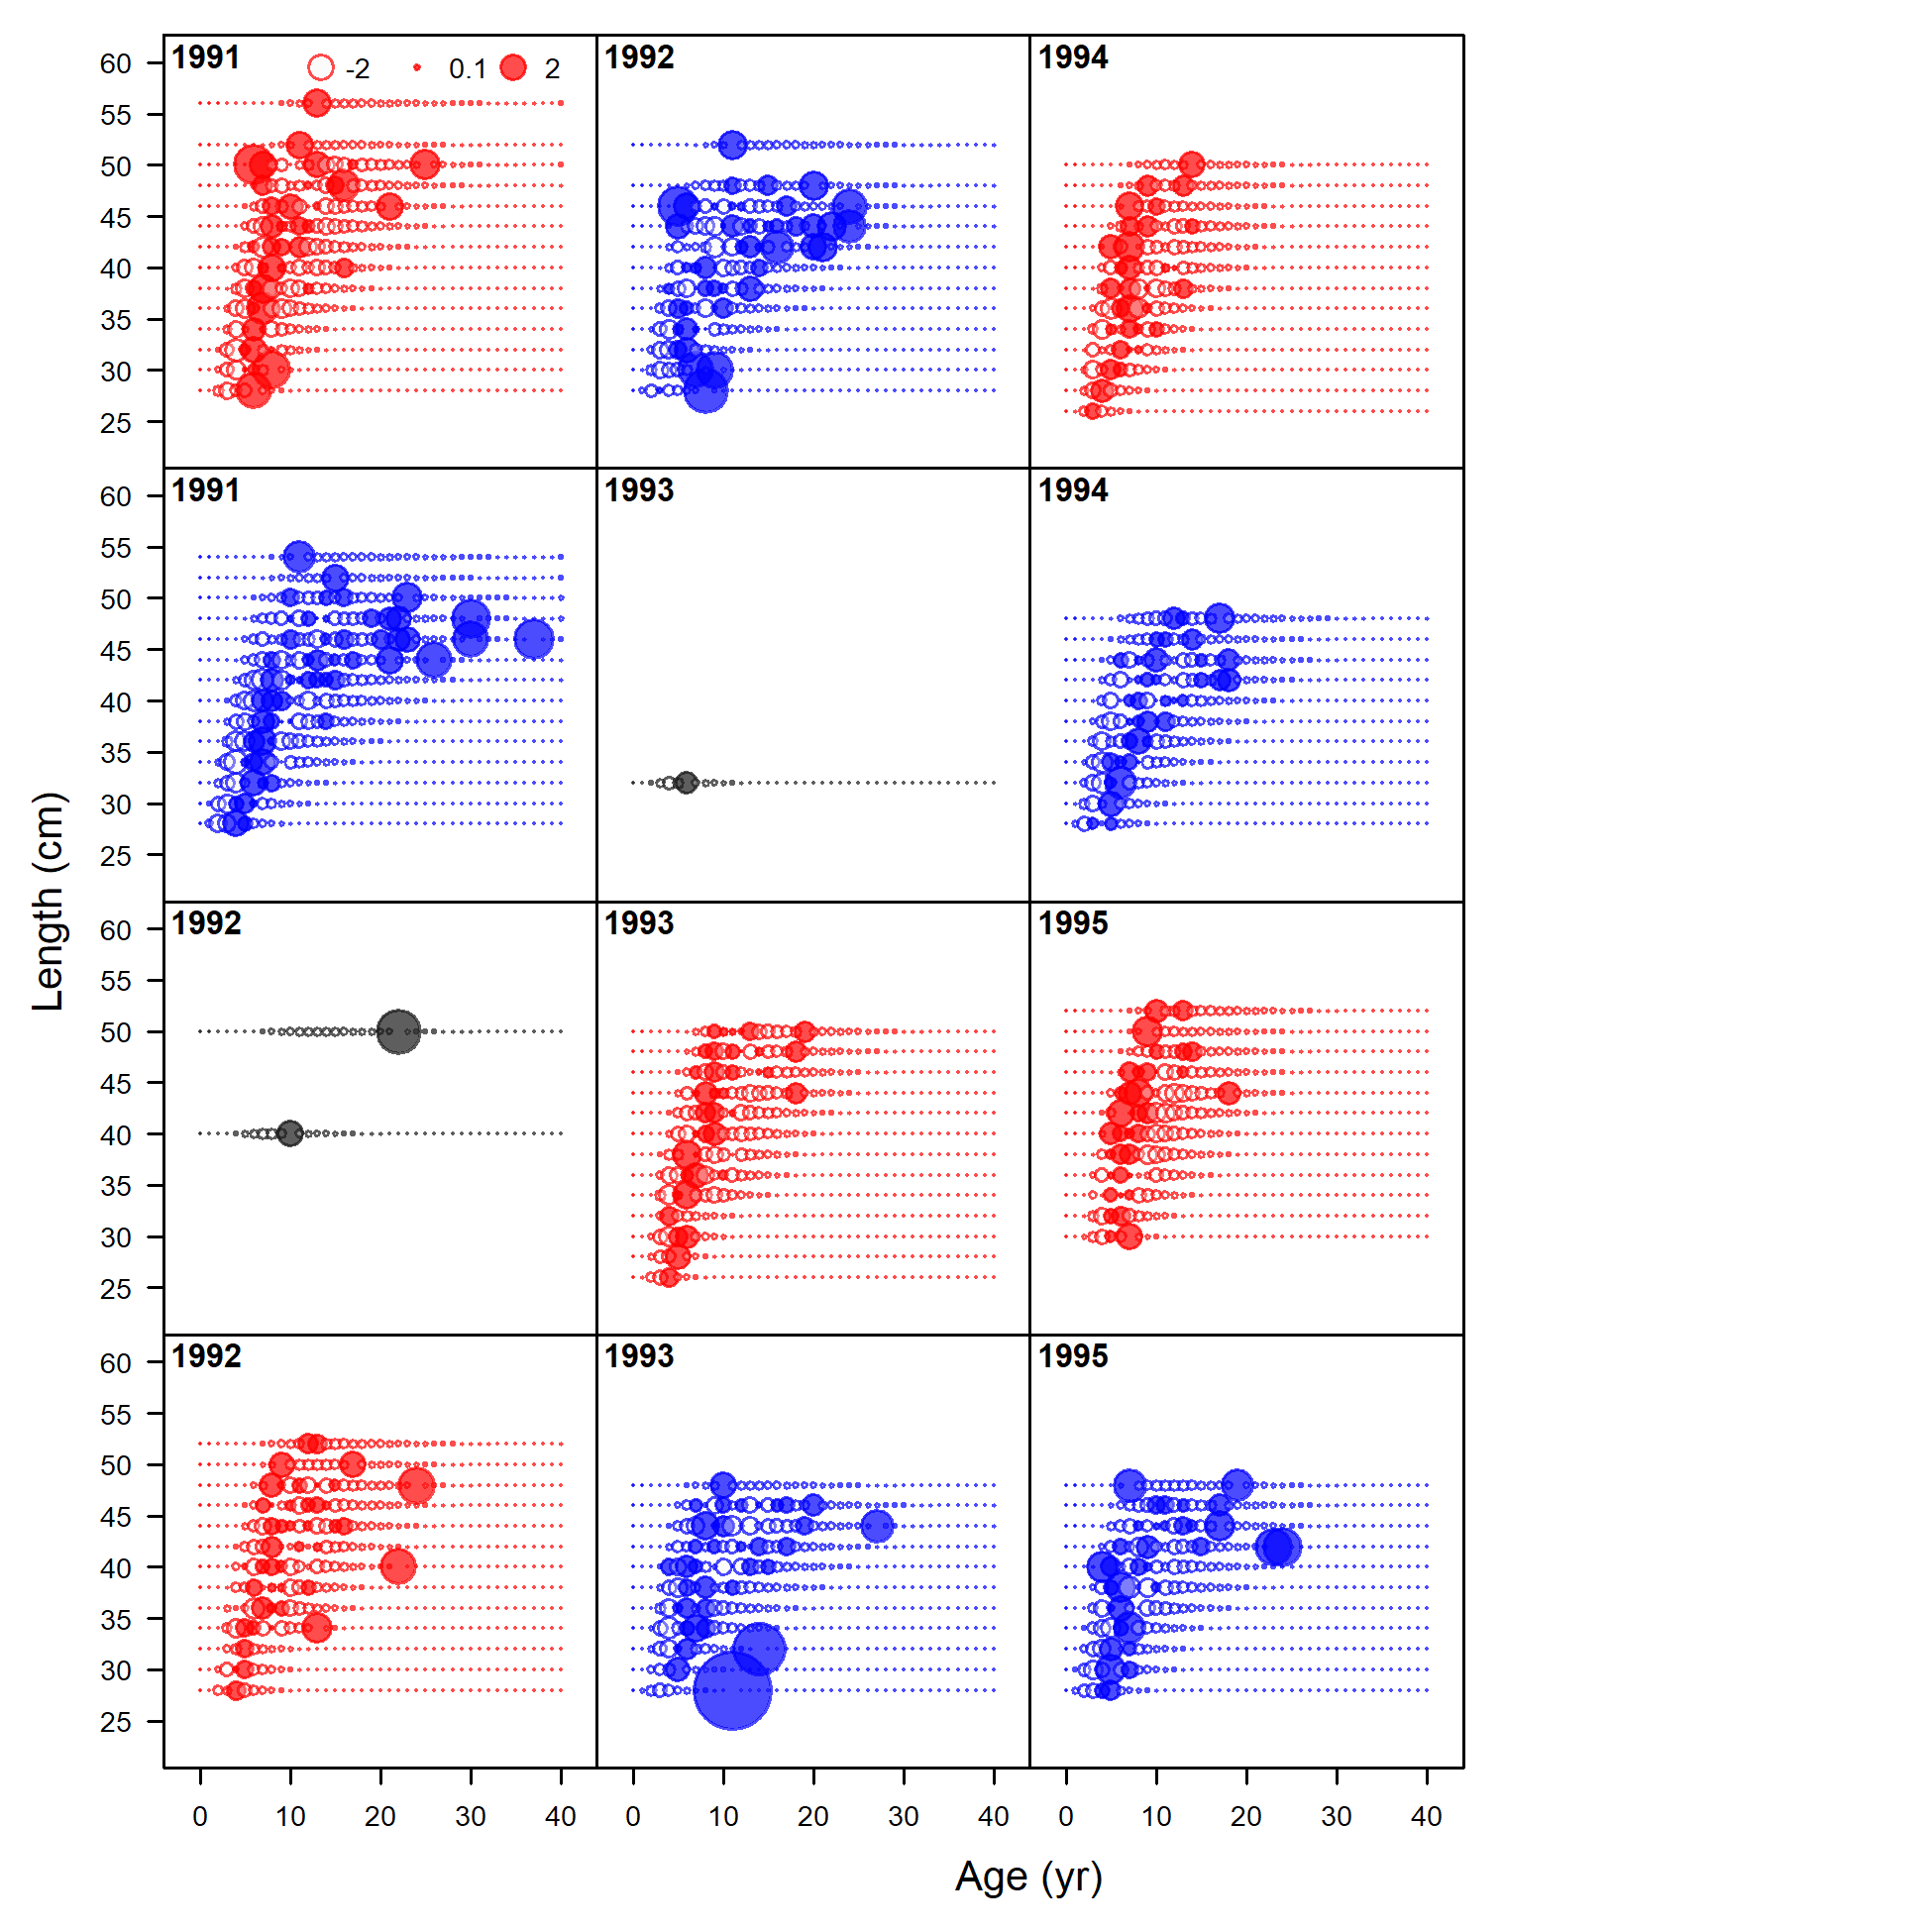
\includegraphics[width=1\textwidth,height=1\textheight]{C:/Users/Jason.Cope/Documents/Github/Sebastes_melanops_WA/Document/models/Reference model/plots/comp_condAALfit_residsflt2mkt0_page2.png}
\caption{Pearson residuals, whole catch, NonTRWL (max=18.54) (plot 2 of 2).\label{fig:comp_condAALfit_residsflt2mkt0_page2}}
\end{figure}

\begin{figure}
\centering
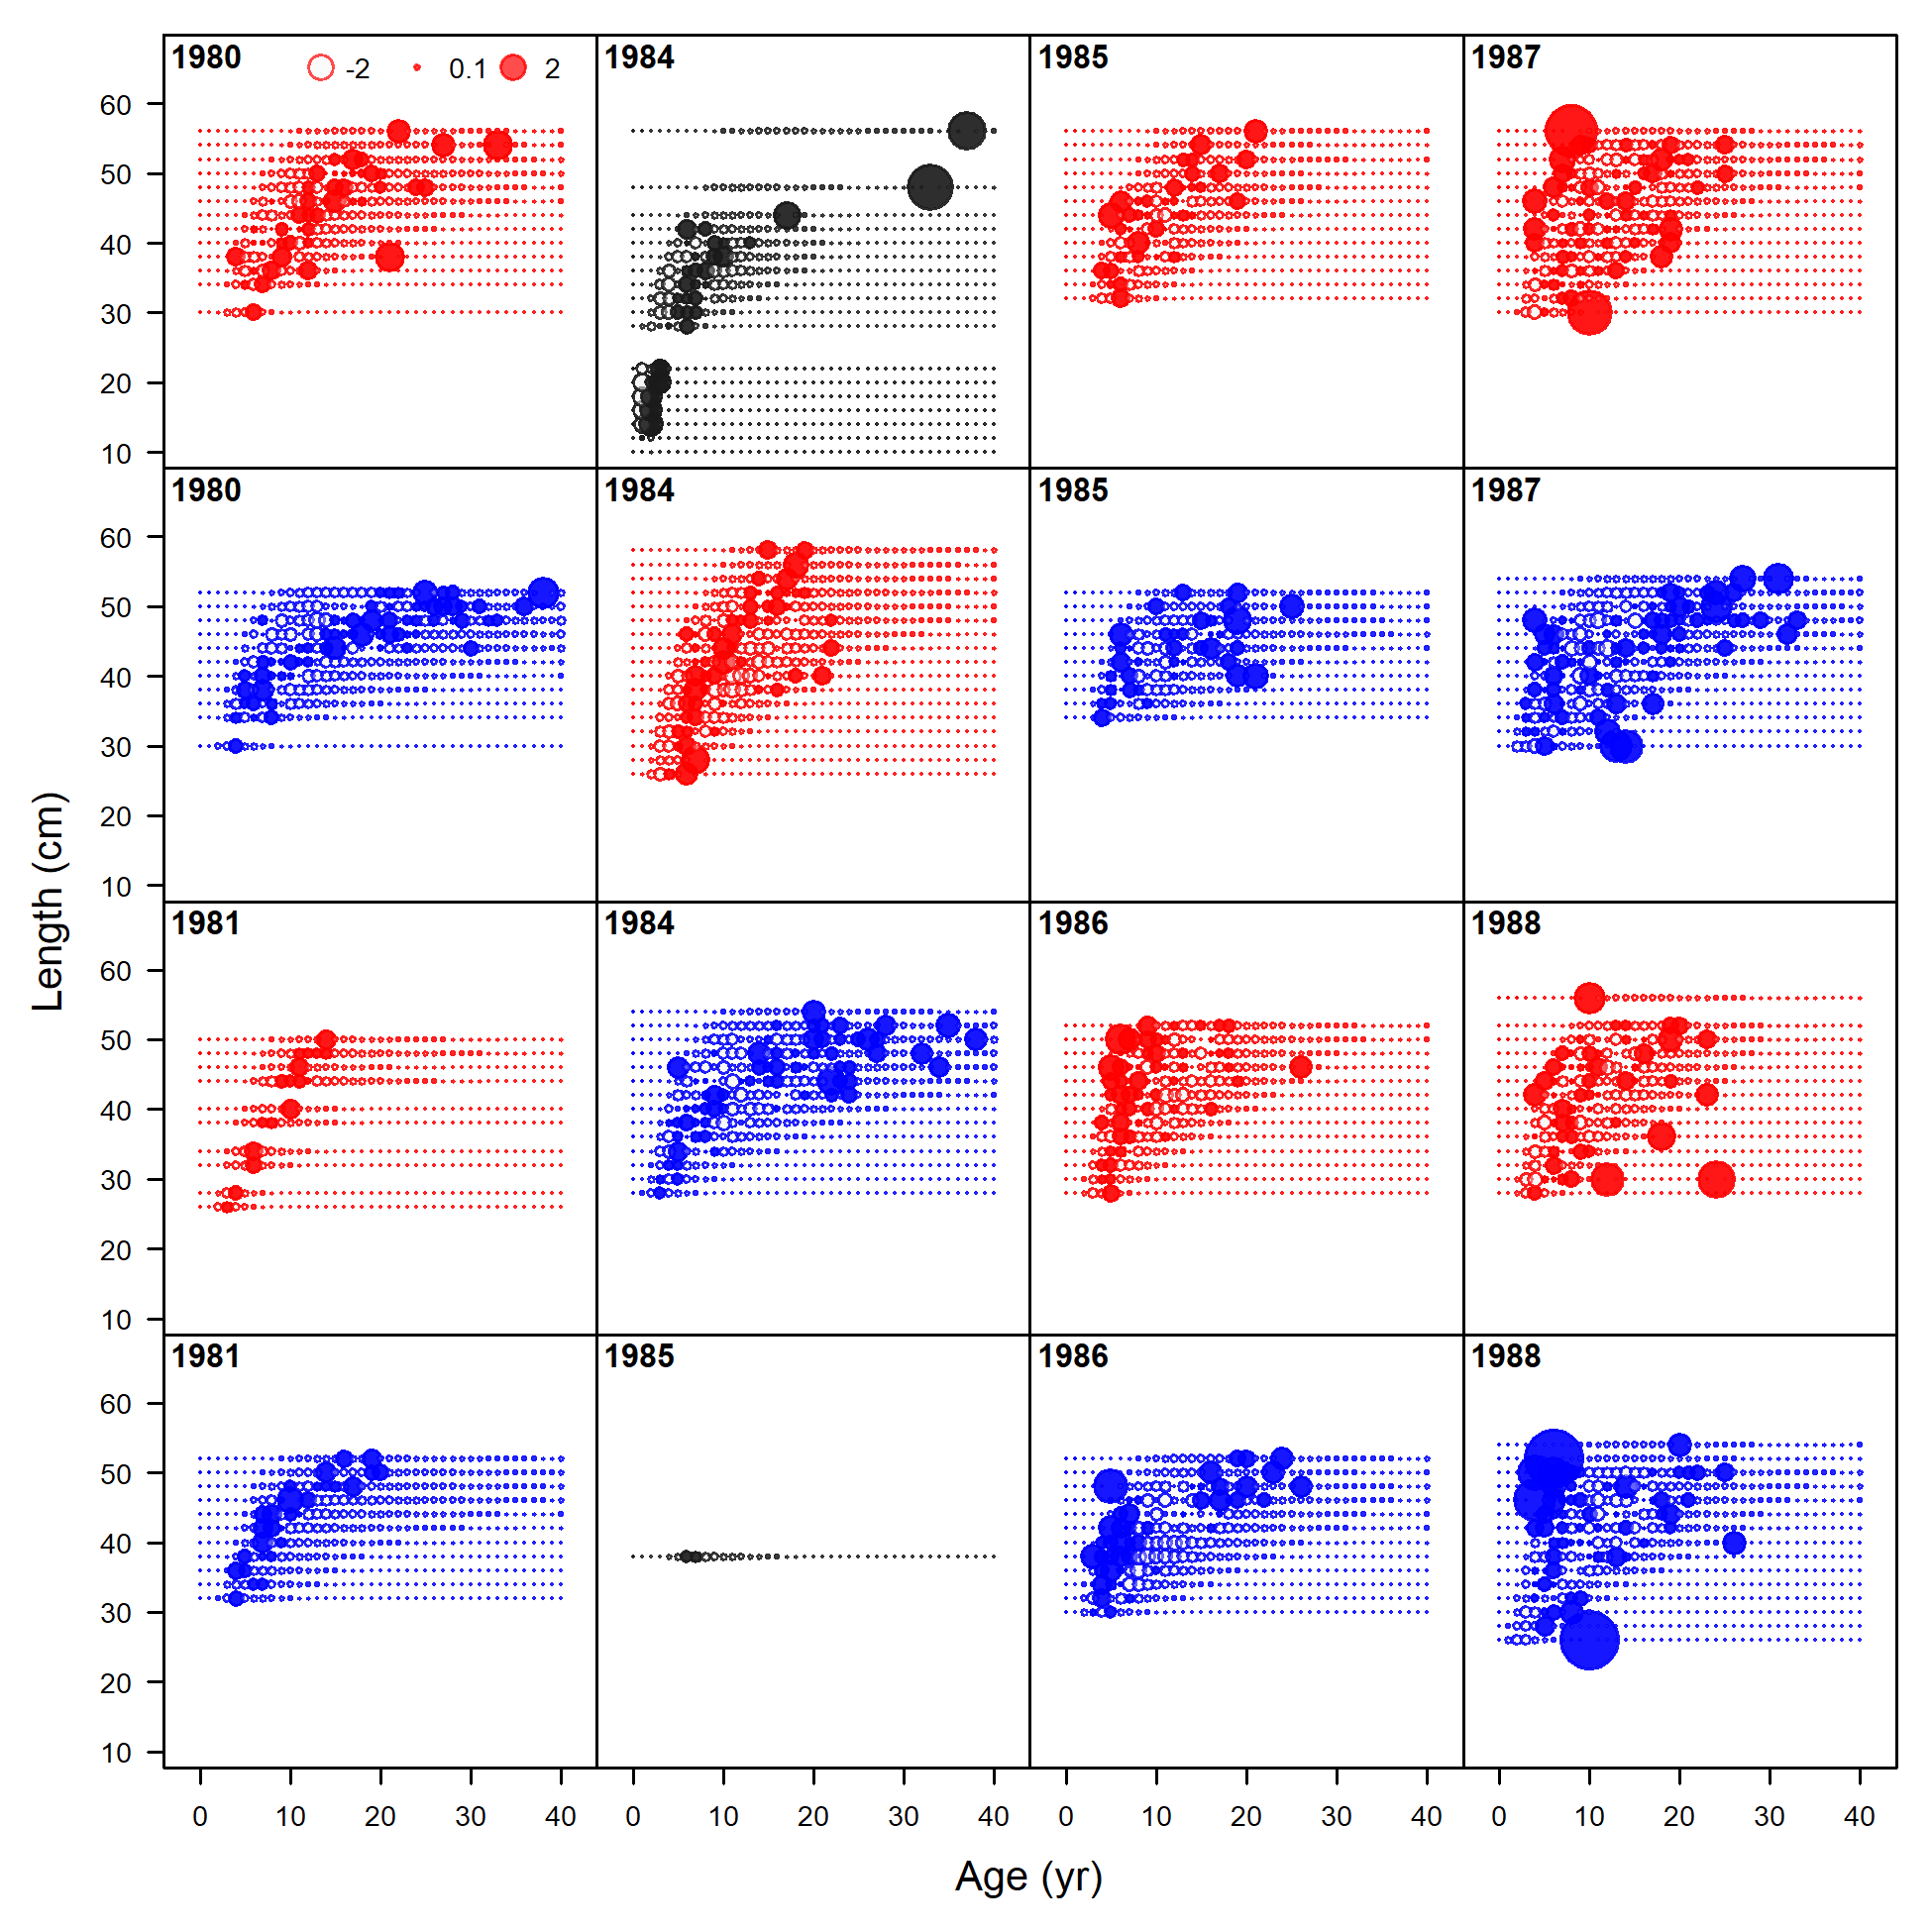
\includegraphics[width=1\textwidth,height=1\textheight]{C:/Users/Jason.Cope/Documents/Github/Sebastes_melanops_WA/Document/models/Reference model/plots/comp_condAALfit_residsflt3mkt0_page1.png}
\caption{Pearson residuals, whole catch, Recreational (max=25.87) (plot 1 of 7).\label{fig:comp_condAALfit_residsflt3mkt0_page1}}
\end{figure}

\begin{figure}
\centering
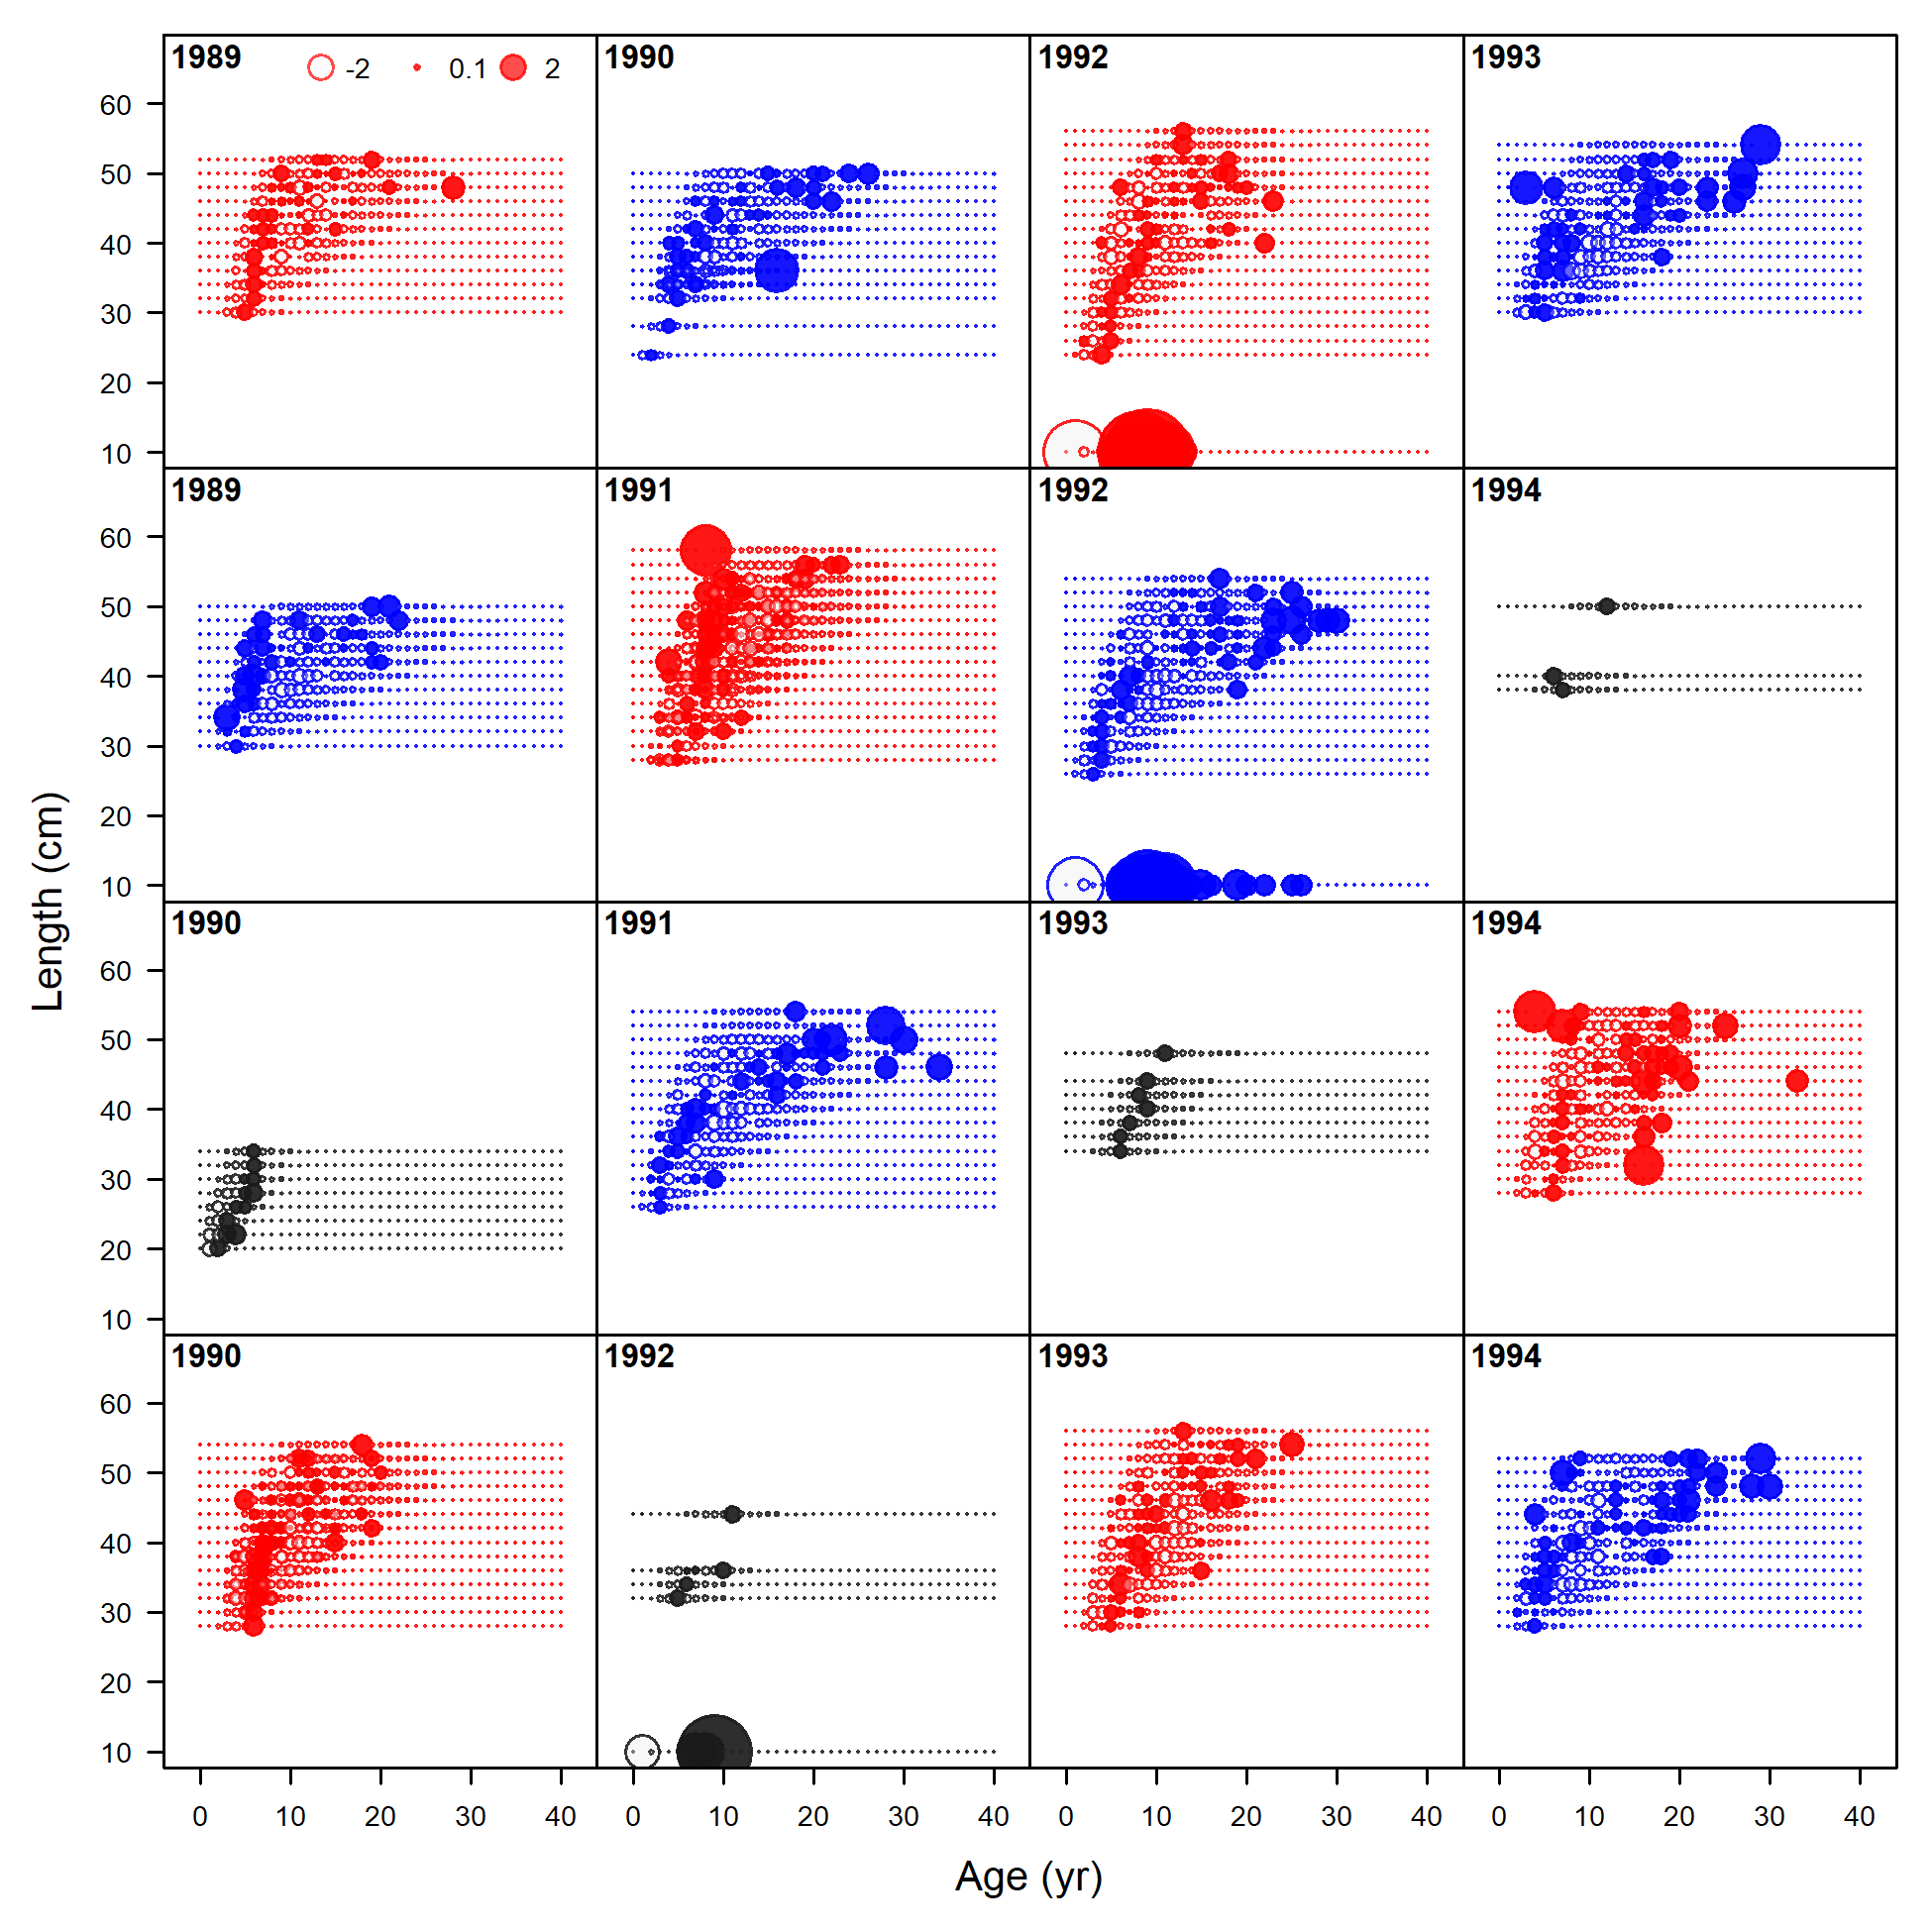
\includegraphics[width=1\textwidth,height=1\textheight]{C:/Users/Jason.Cope/Documents/Github/Sebastes_melanops_WA/Document/models/Reference model/plots/comp_condAALfit_residsflt3mkt0_page2.png}
\caption{Pearson residuals, whole catch, Recreational (max=25.87) (plot 2 of 7).\label{fig:comp_condAALfit_residsflt3mkt0_page2}}
\end{figure}

\begin{figure}
\centering
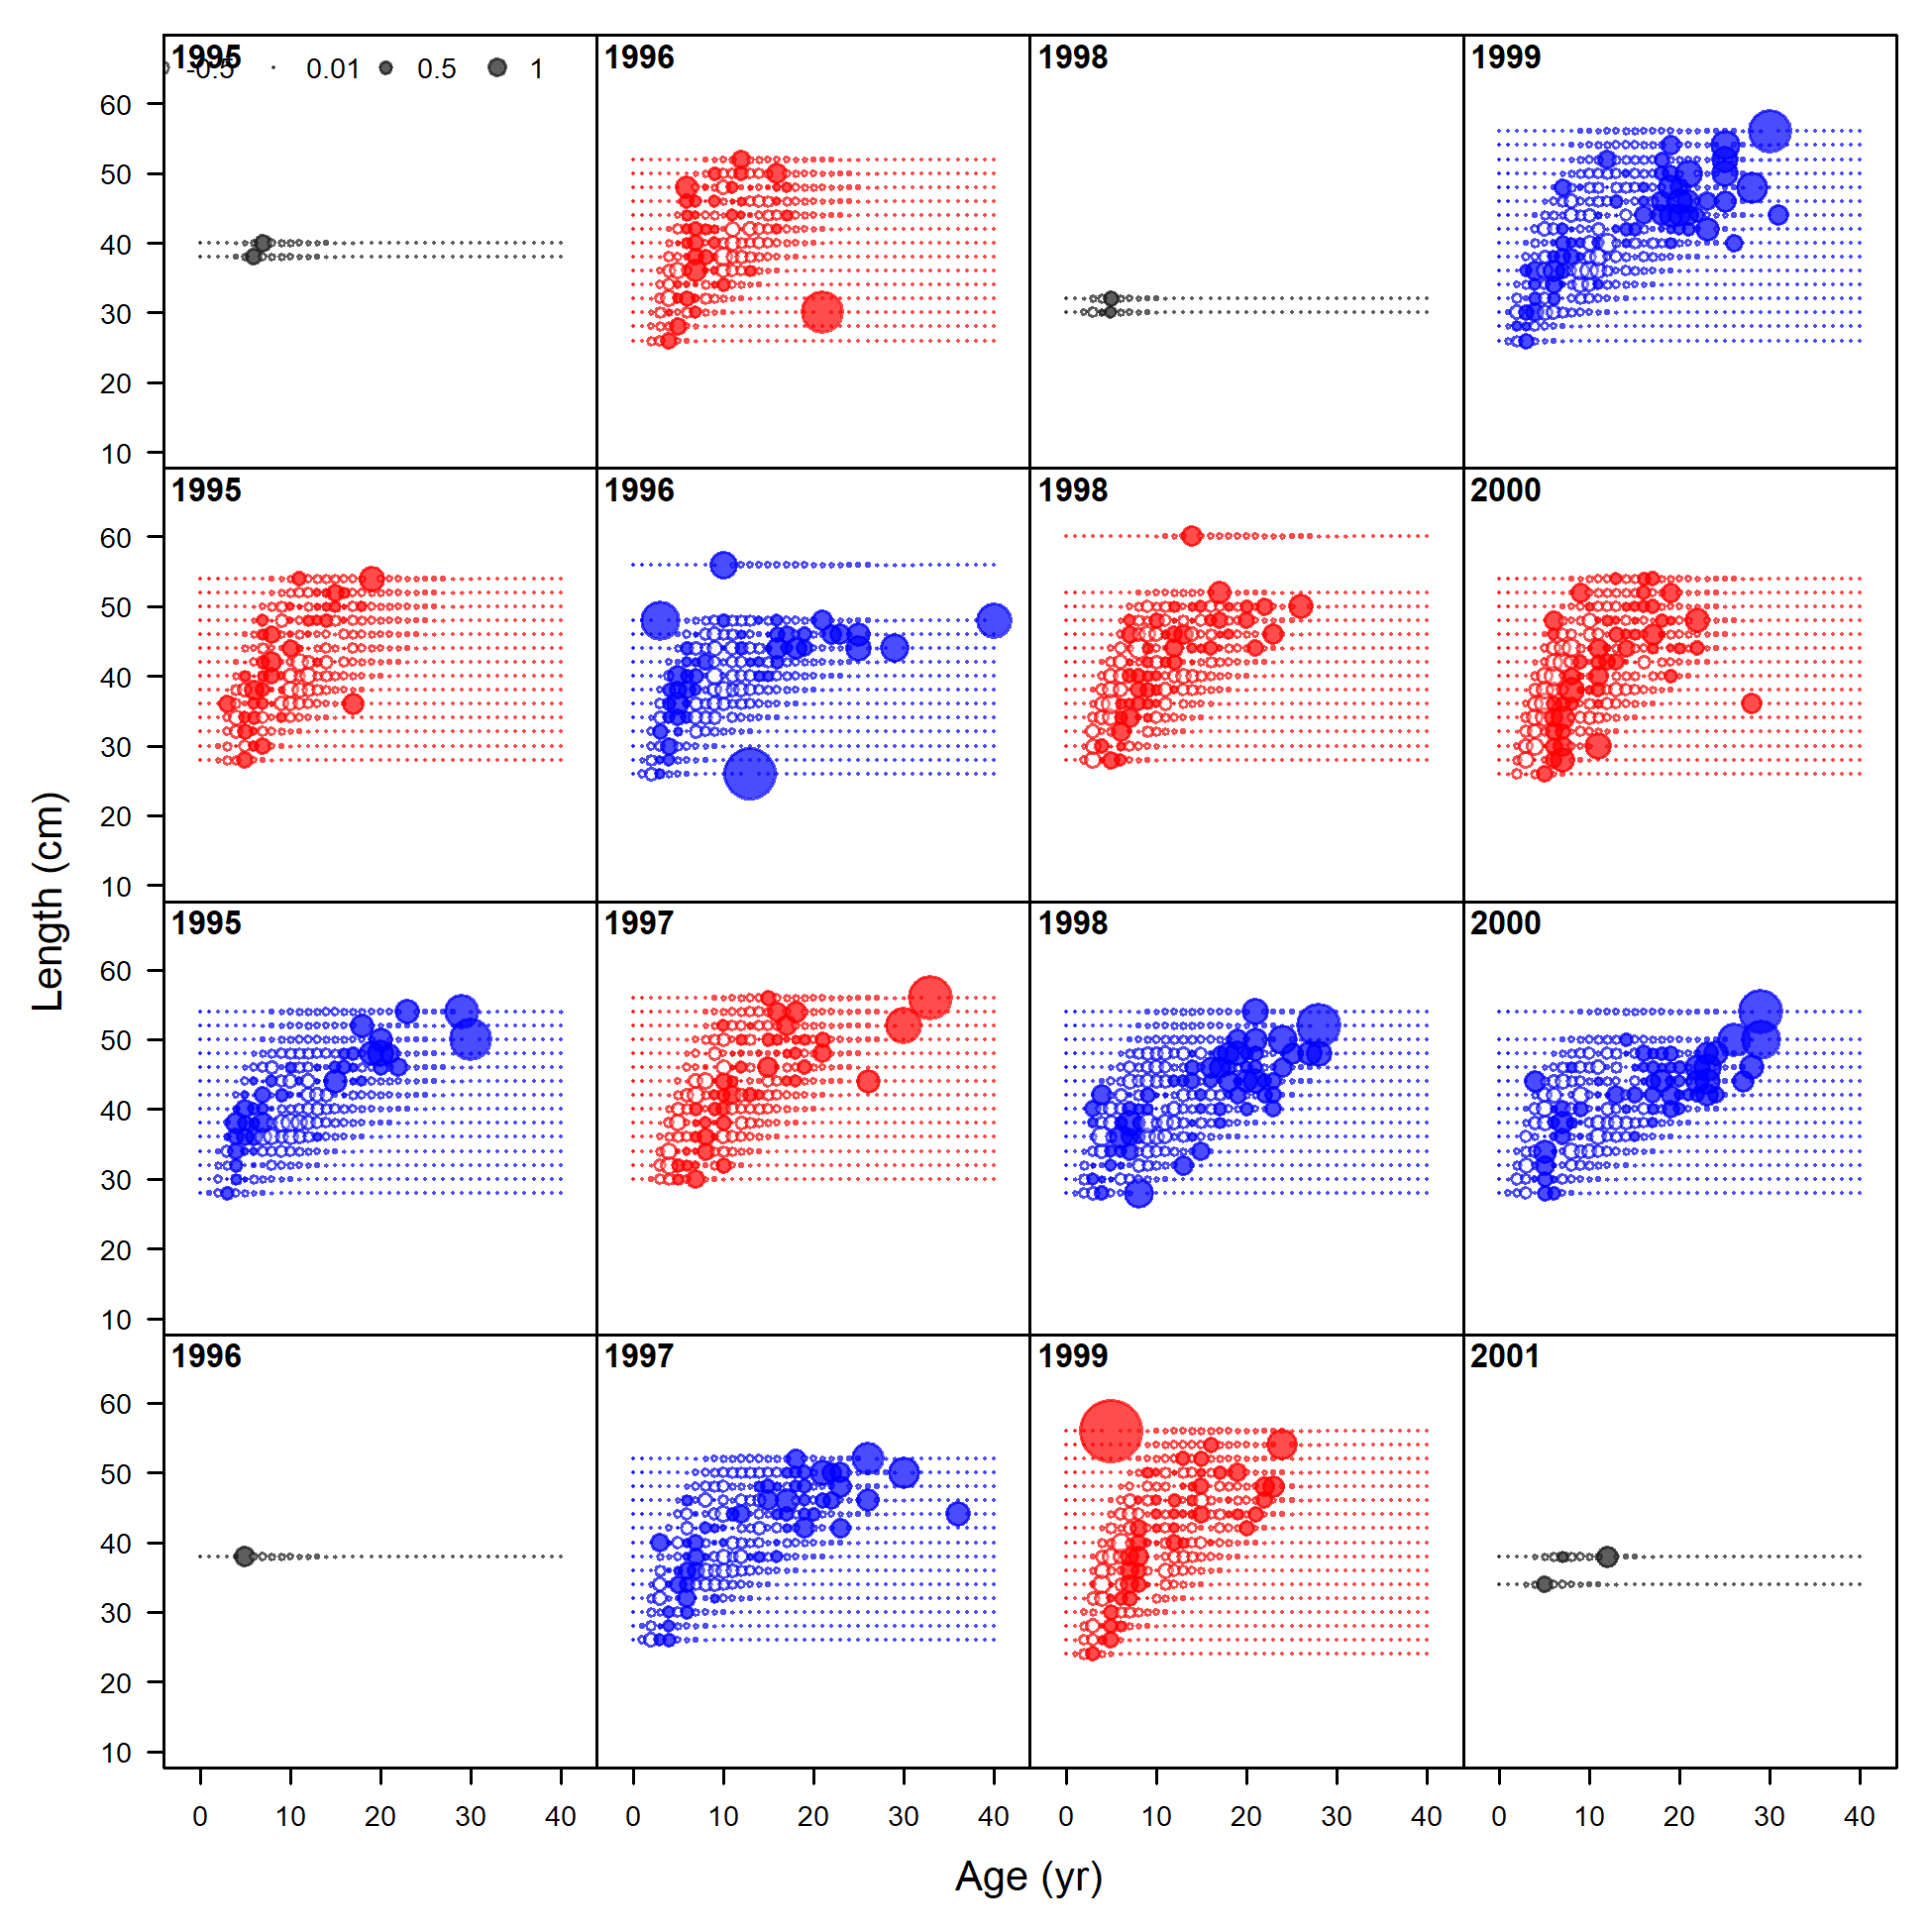
\includegraphics[width=1\textwidth,height=1\textheight]{C:/Users/Jason.Cope/Documents/Github/Sebastes_melanops_WA/Document/models/Reference model/plots/comp_condAALfit_residsflt3mkt0_page3.png}
\caption{Pearson residuals, whole catch, Recreational (max=25.87) (plot 3 of 7).\label{fig:comp_condAALfit_residsflt3mkt0_page3}}
\end{figure}

\begin{figure}
\centering
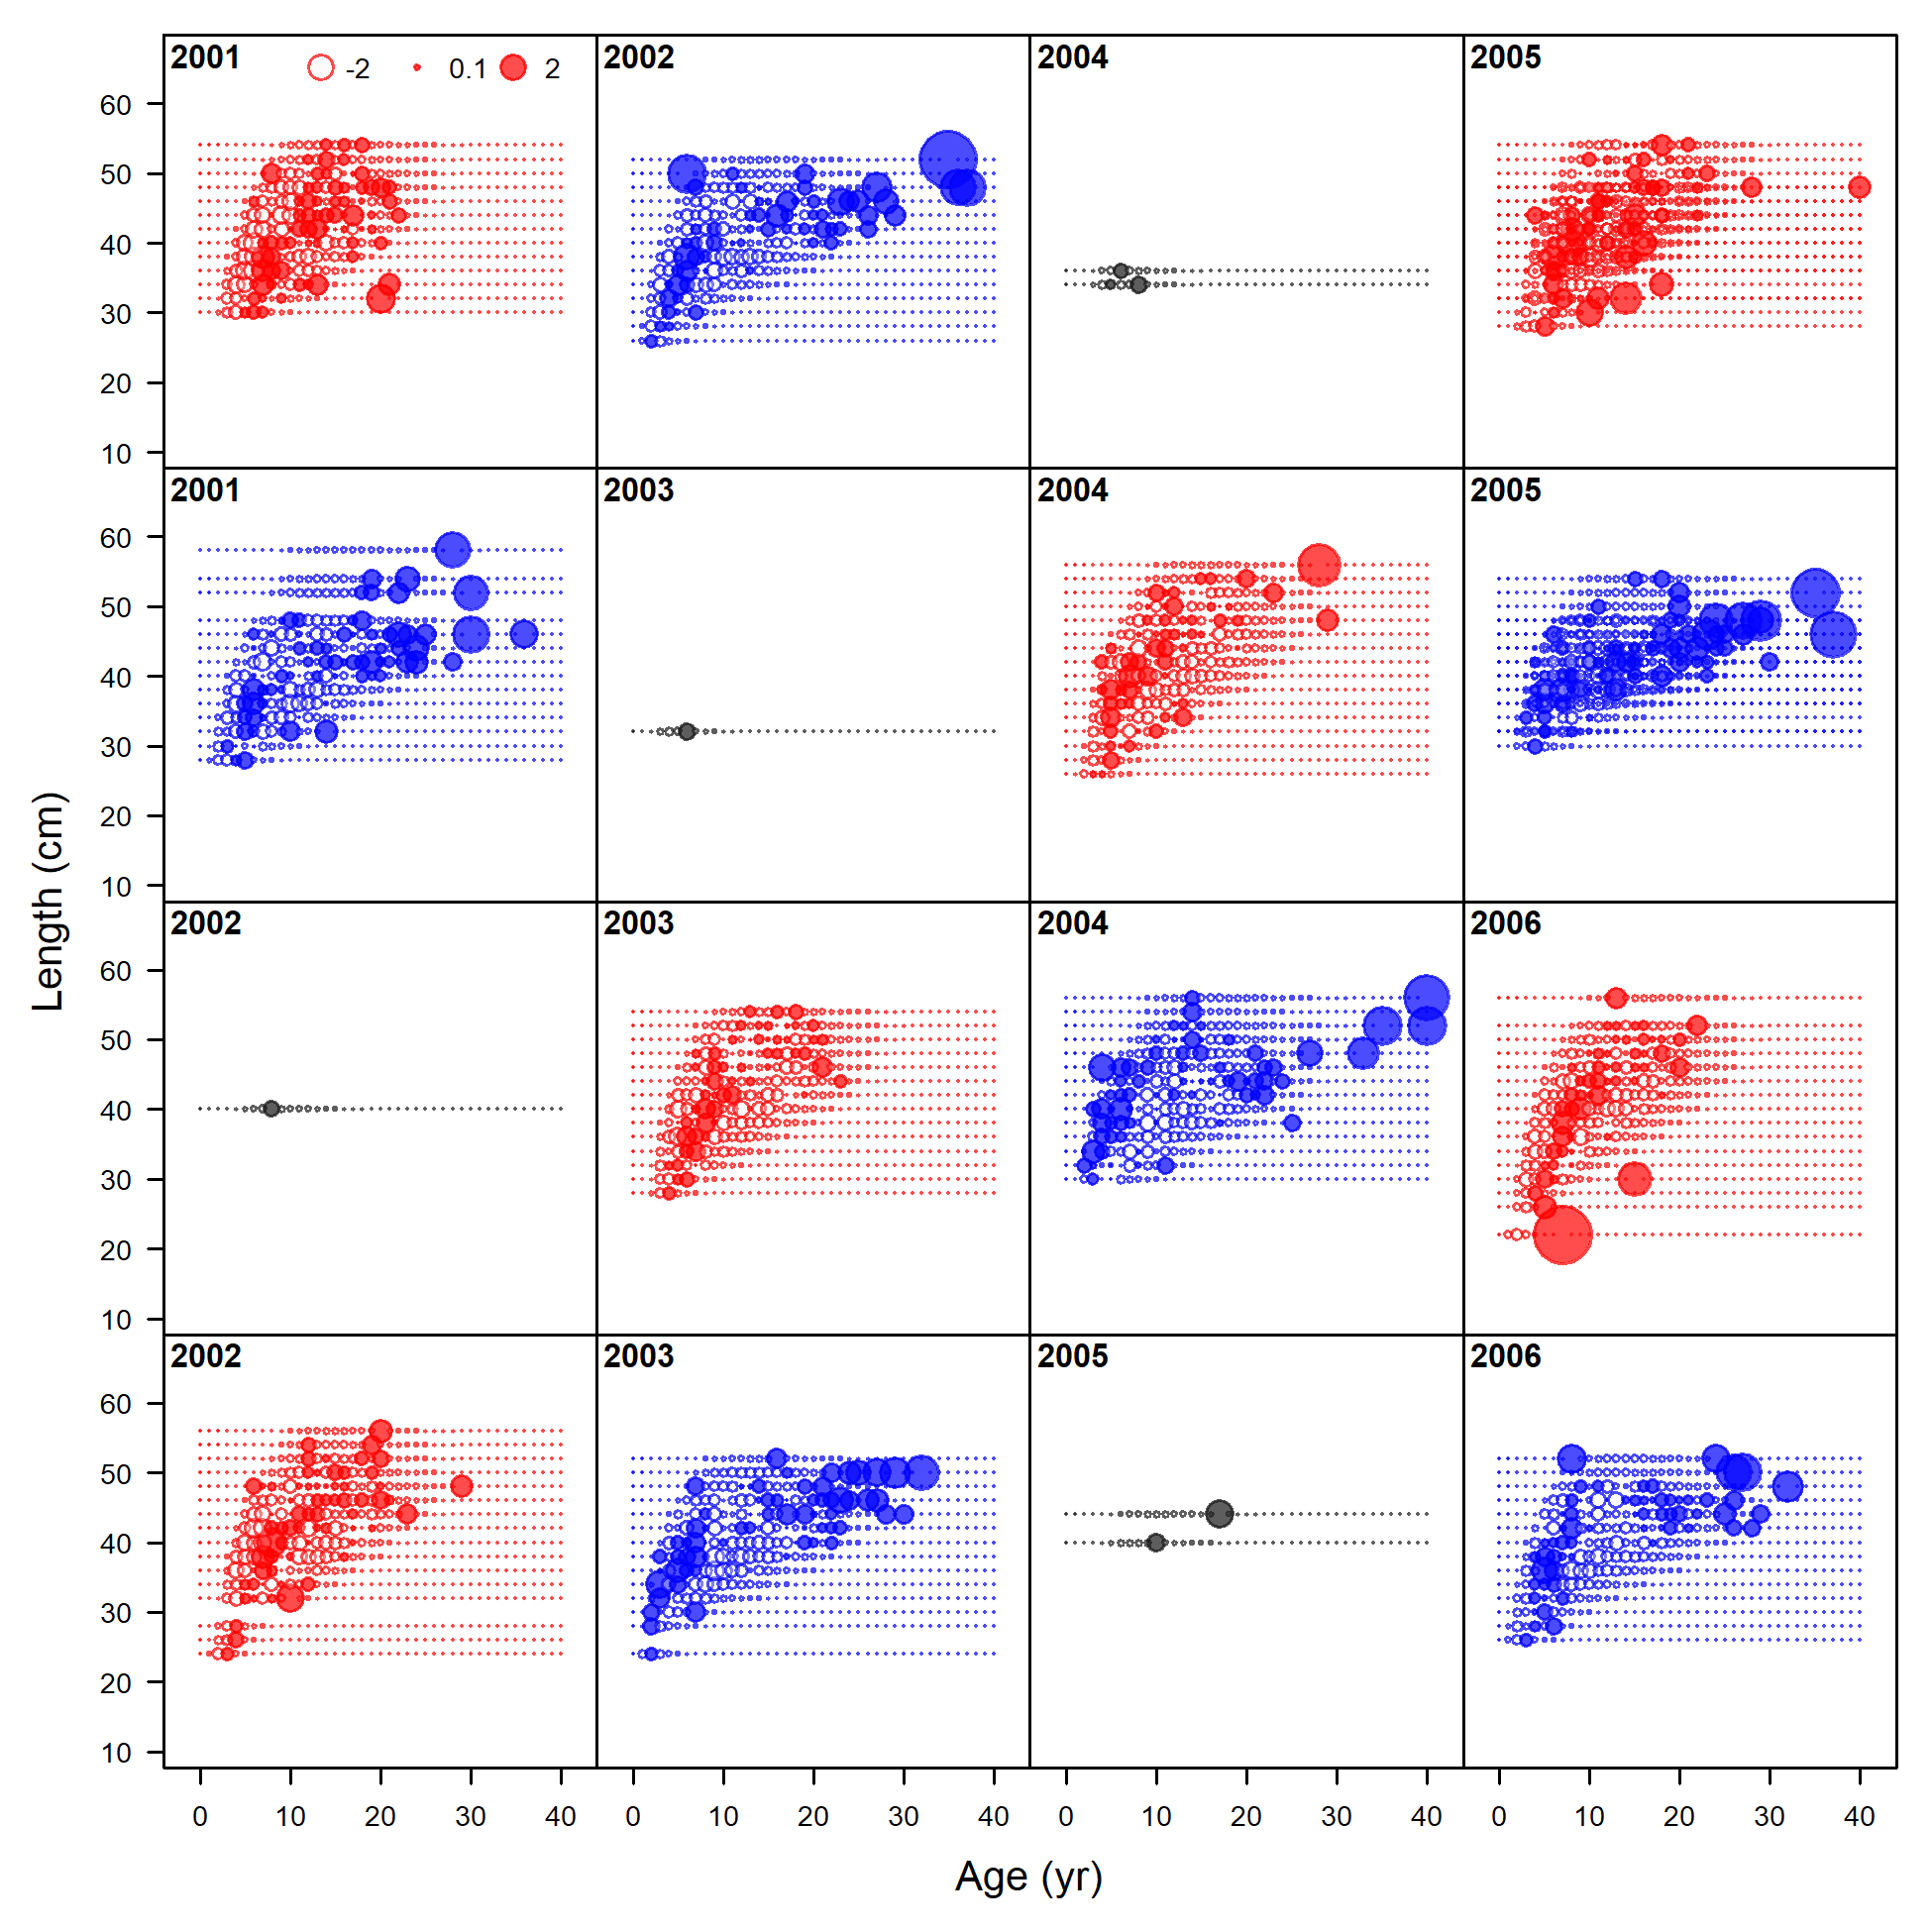
\includegraphics[width=1\textwidth,height=1\textheight]{C:/Users/Jason.Cope/Documents/Github/Sebastes_melanops_WA/Document/models/Reference model/plots/comp_condAALfit_residsflt3mkt0_page4.png}
\caption{Pearson residuals, whole catch, Recreational (max=25.87) (plot 4 of 7).\label{fig:comp_condAALfit_residsflt3mkt0_page4}}
\end{figure}

\begin{figure}
\centering
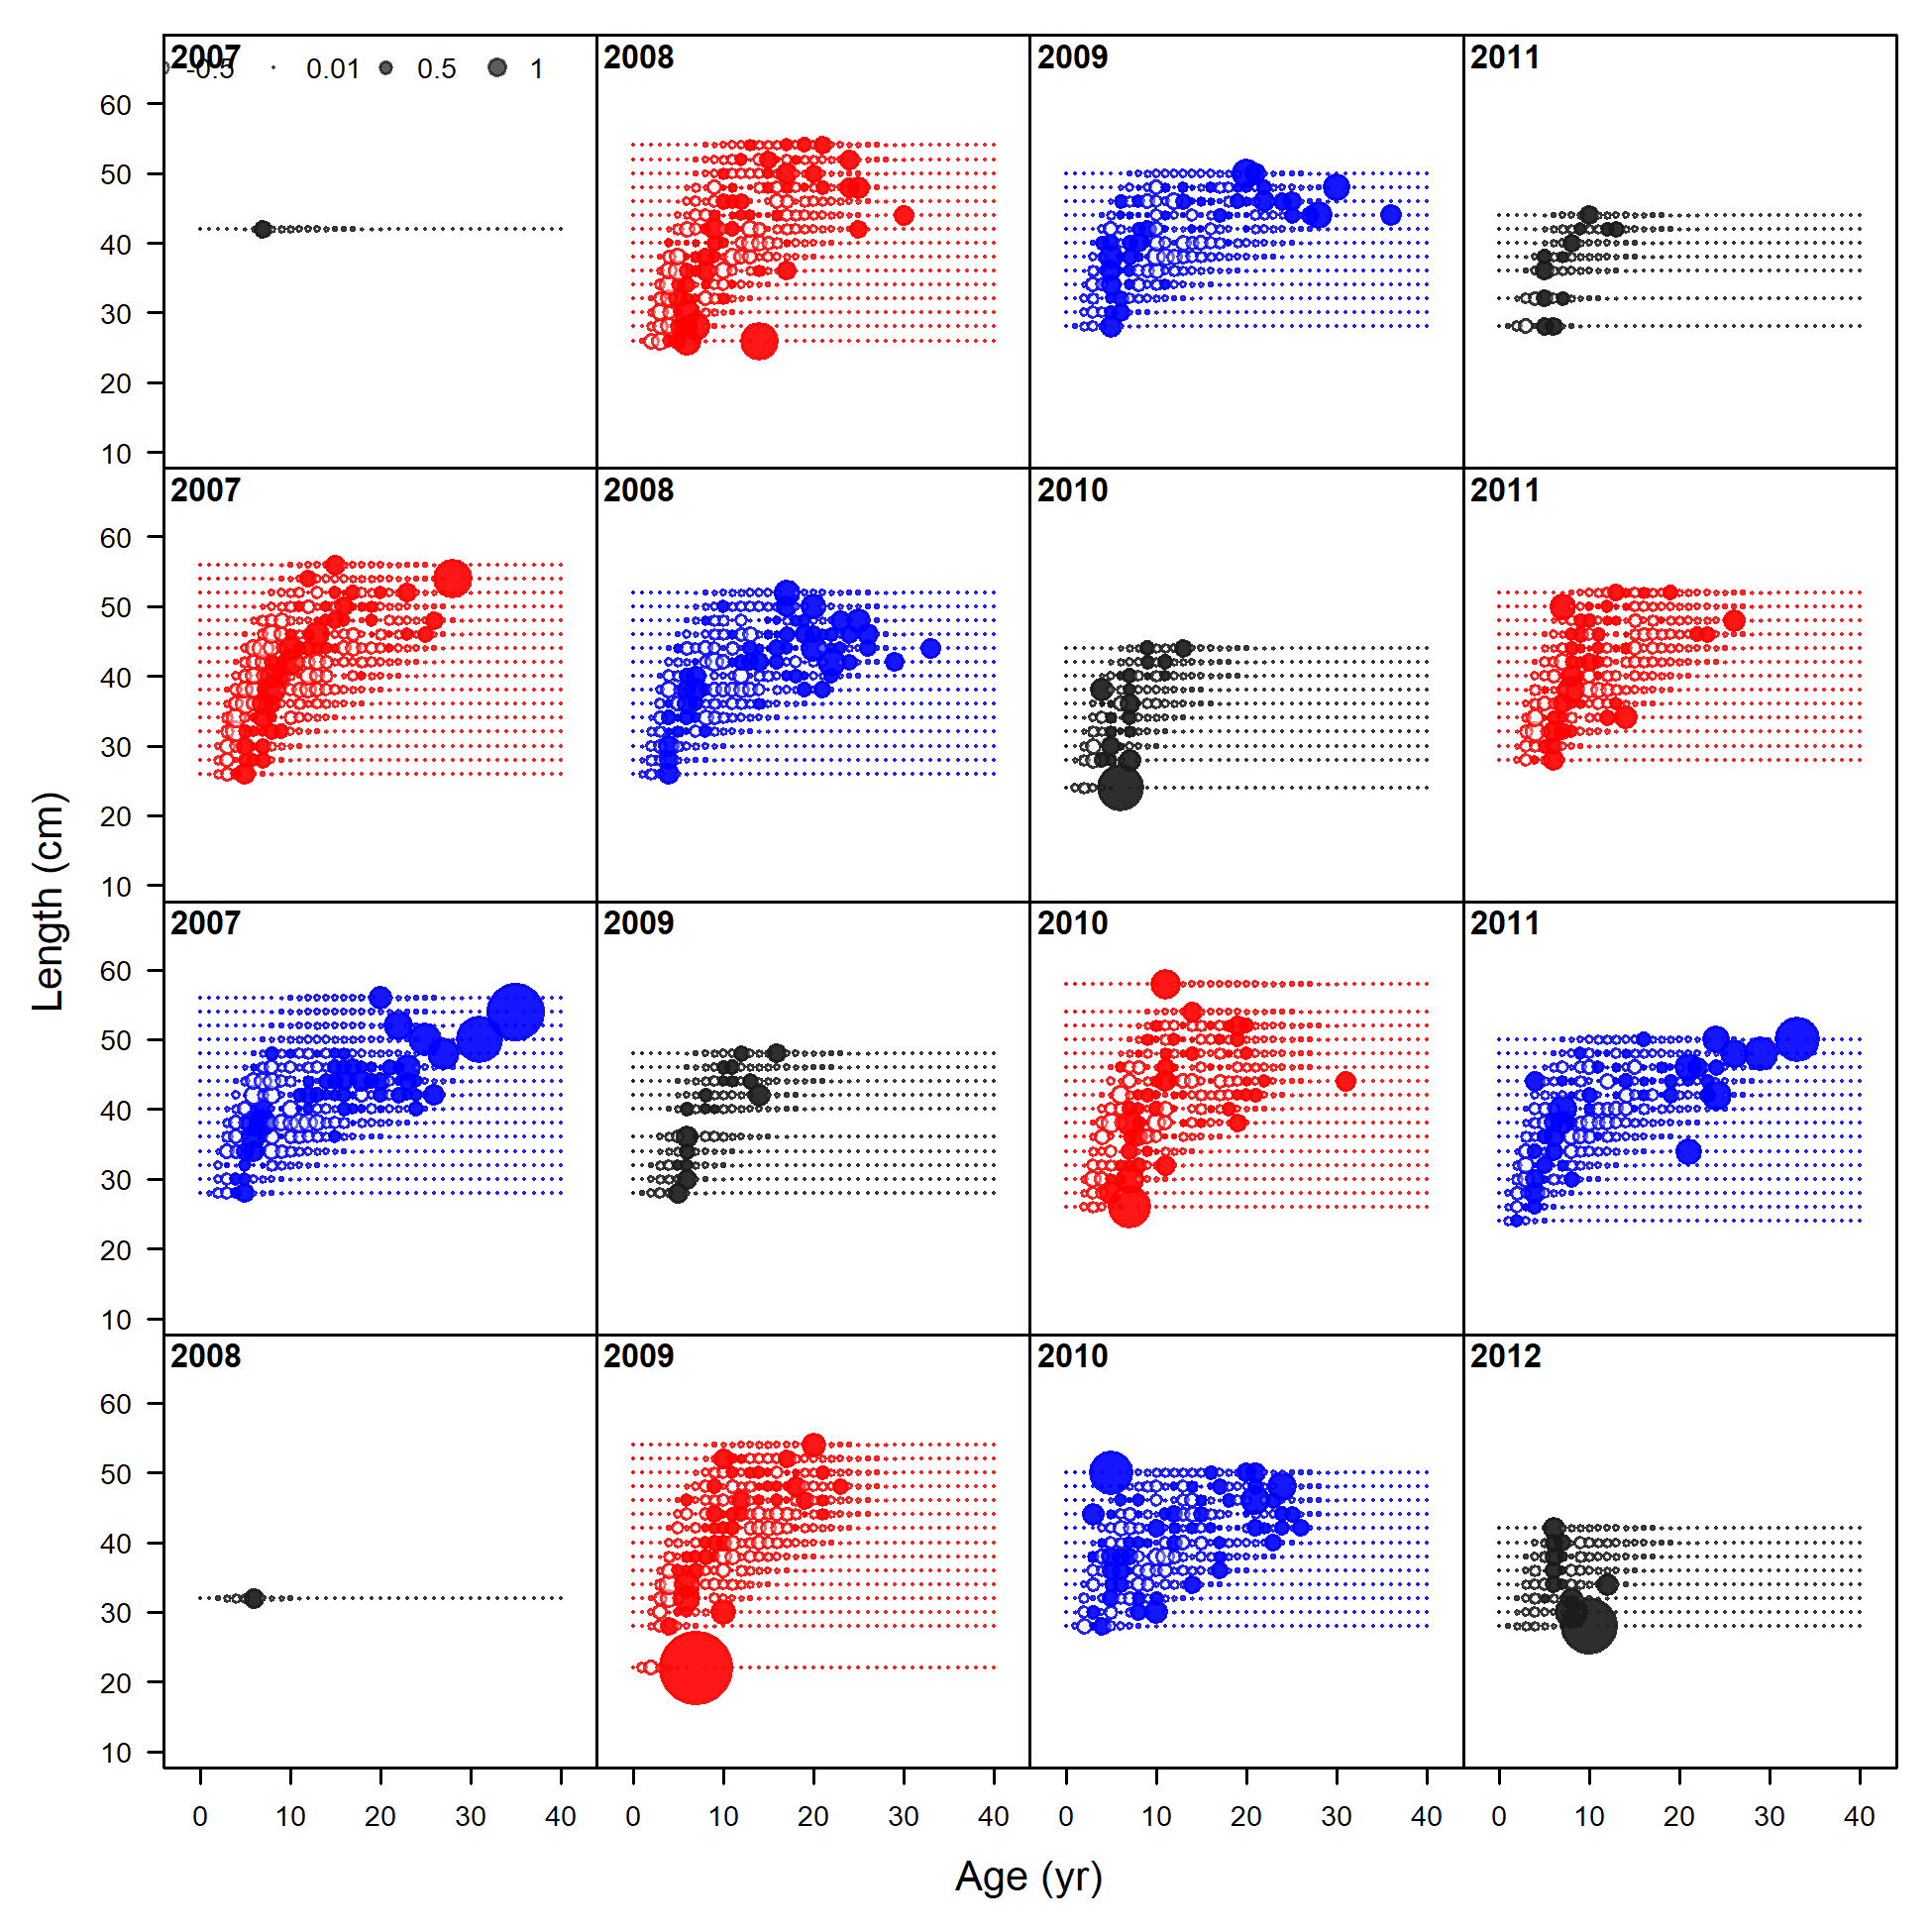
\includegraphics[width=1\textwidth,height=1\textheight]{C:/Users/Jason.Cope/Documents/Github/Sebastes_melanops_WA/Document/models/Reference model/plots/comp_condAALfit_residsflt3mkt0_page5.png}
\caption{Pearson residuals, whole catch, Recreational (max=25.87) (plot 5 of 7).\label{fig:comp_condAALfit_residsflt3mkt0_page5}}
\end{figure}

\begin{figure}
\centering
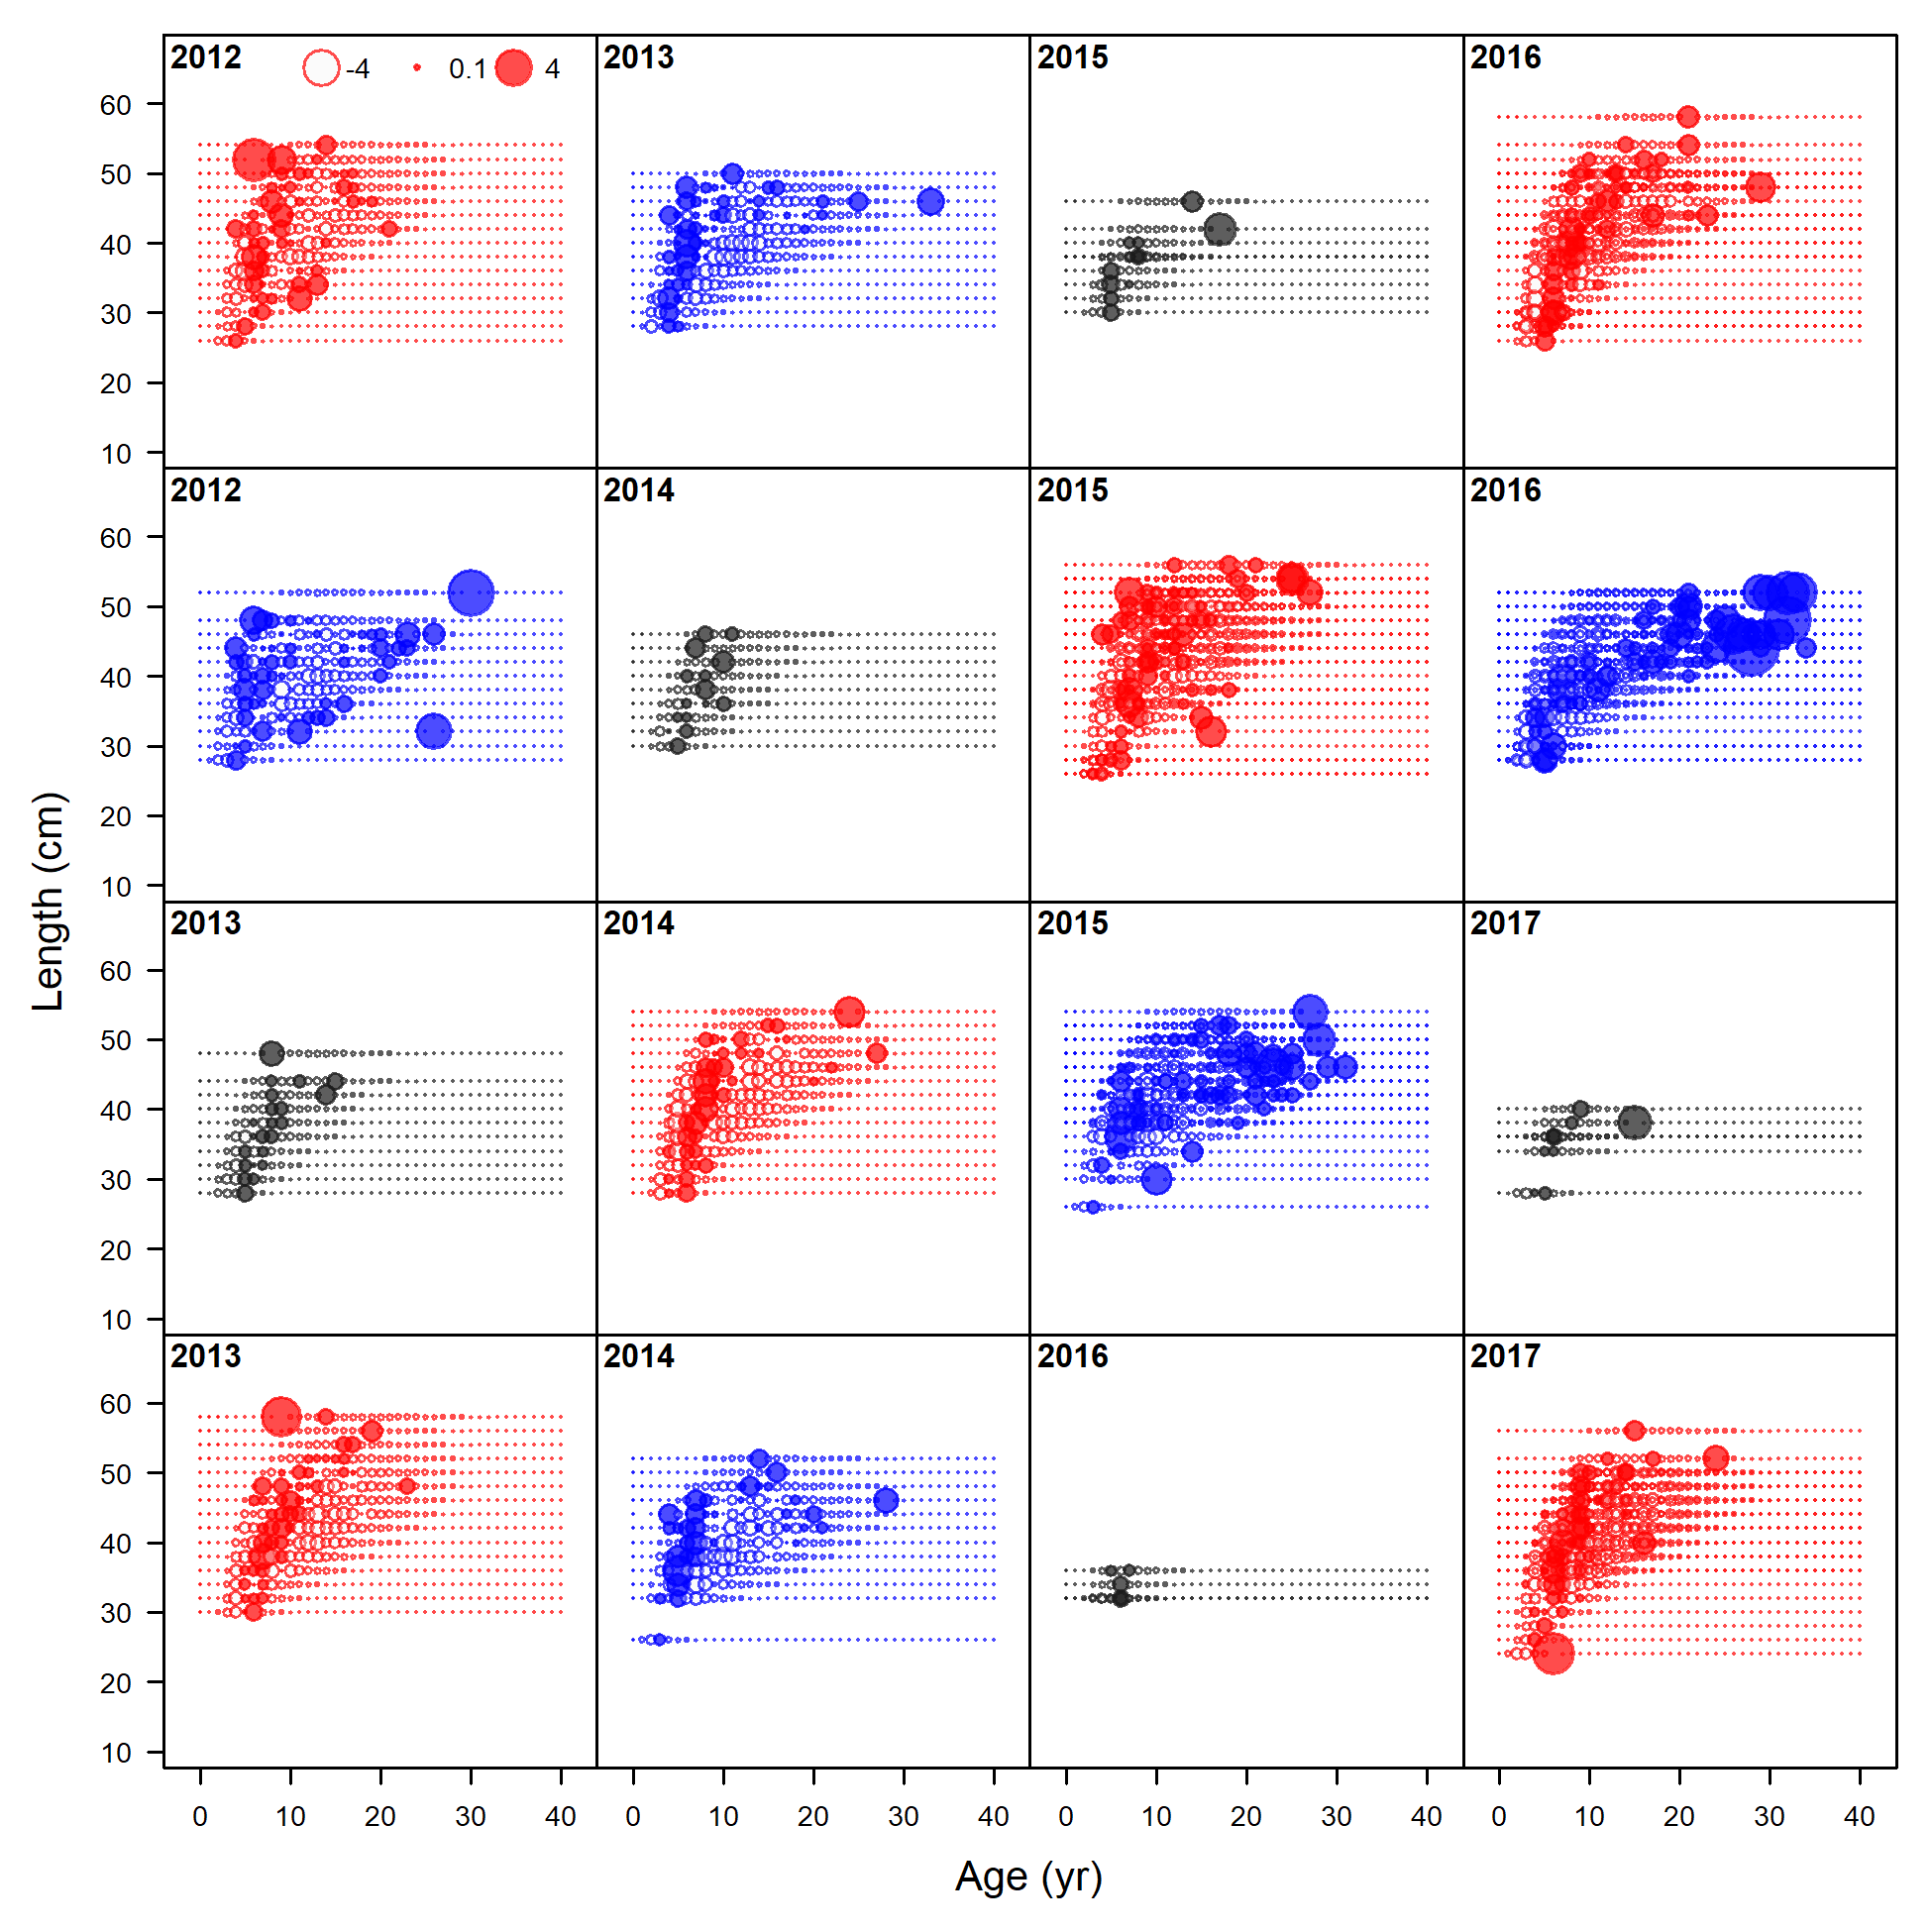
\includegraphics[width=1\textwidth,height=1\textheight]{C:/Users/Jason.Cope/Documents/Github/Sebastes_melanops_WA/Document/models/Reference model/plots/comp_condAALfit_residsflt3mkt0_page6.png}
\caption{Pearson residuals, whole catch, Recreational (max=25.87) (plot 6 of 7).\label{fig:comp_condAALfit_residsflt3mkt0_page6}}
\end{figure}

\begin{figure}
\centering
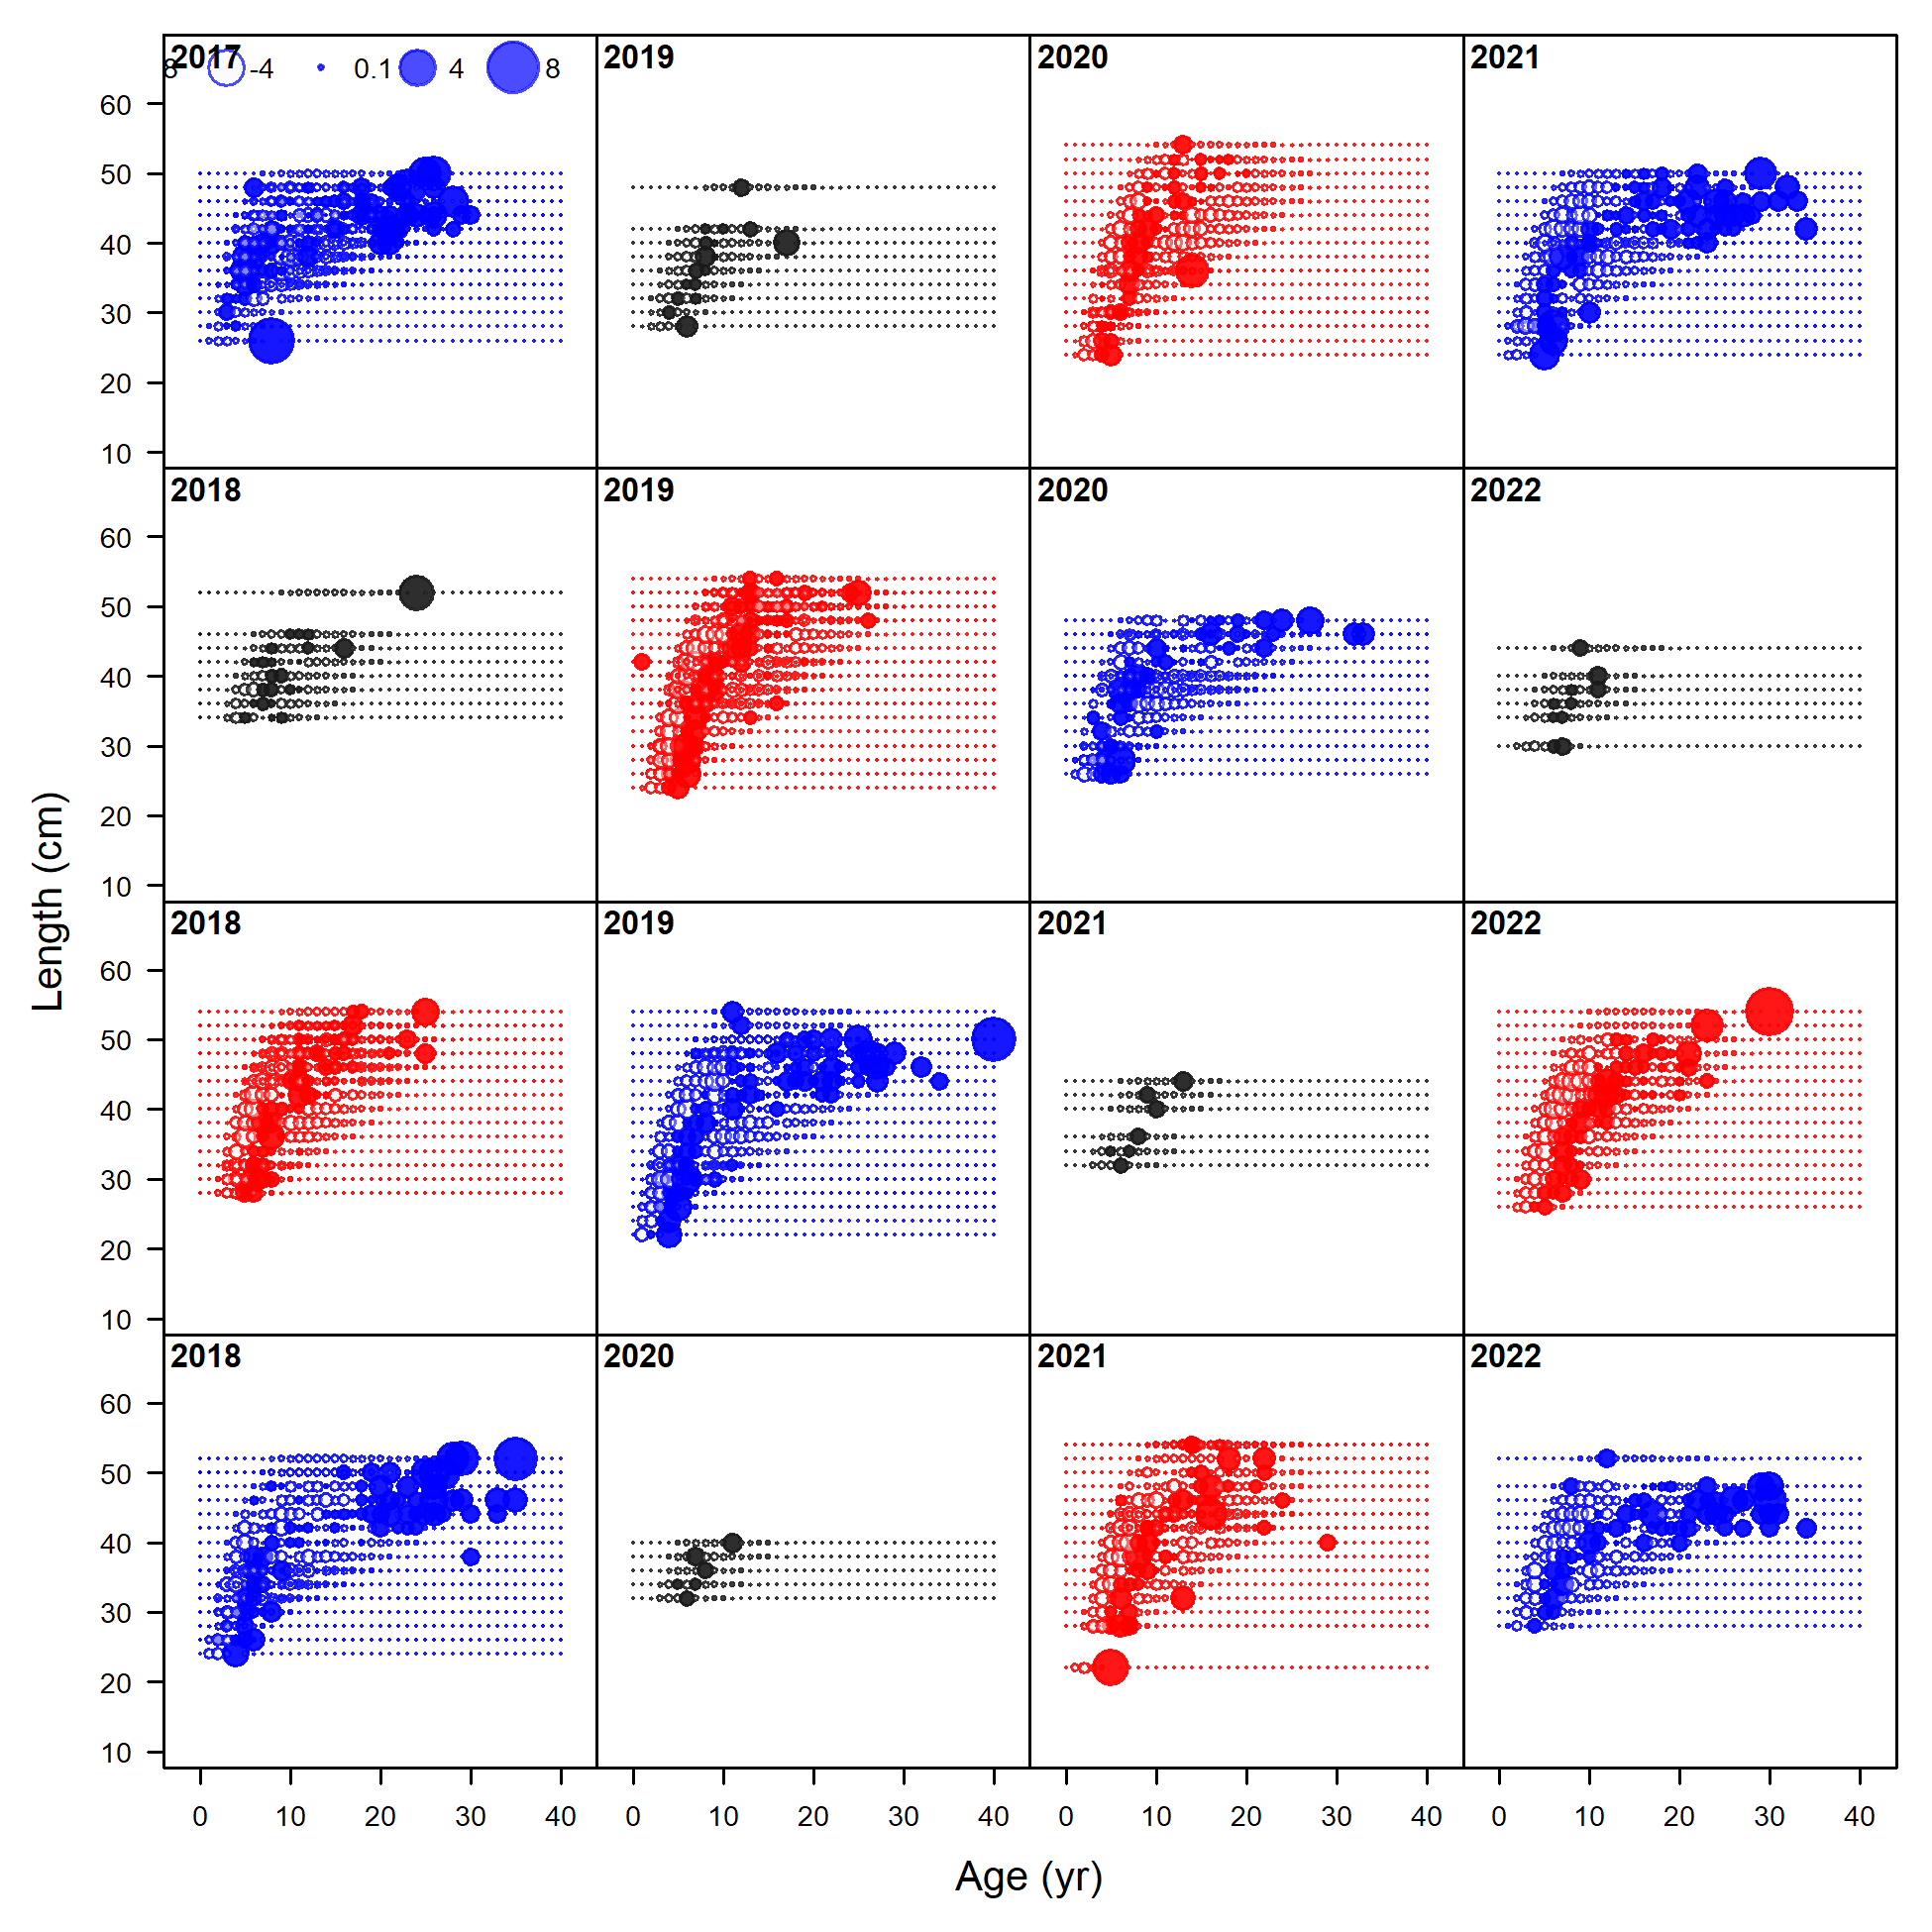
\includegraphics[width=1\textwidth,height=1\textheight]{C:/Users/Jason.Cope/Documents/Github/Sebastes_melanops_WA/Document/models/Reference model/plots/comp_condAALfit_residsflt3mkt0_page7.png}
\caption{Pearson residuals, whole catch, Recreational (max=25.87) (plot 7 of 7).\label{fig:comp_condAALfit_residsflt3mkt0_page7}}
\end{figure}

\clearpage

\hypertarget{app-c}{%
\section{Appendix C: Fit to Conditional-Age-at-Length Composition Data}\label{app-c}}

\begin{figure}
\centering
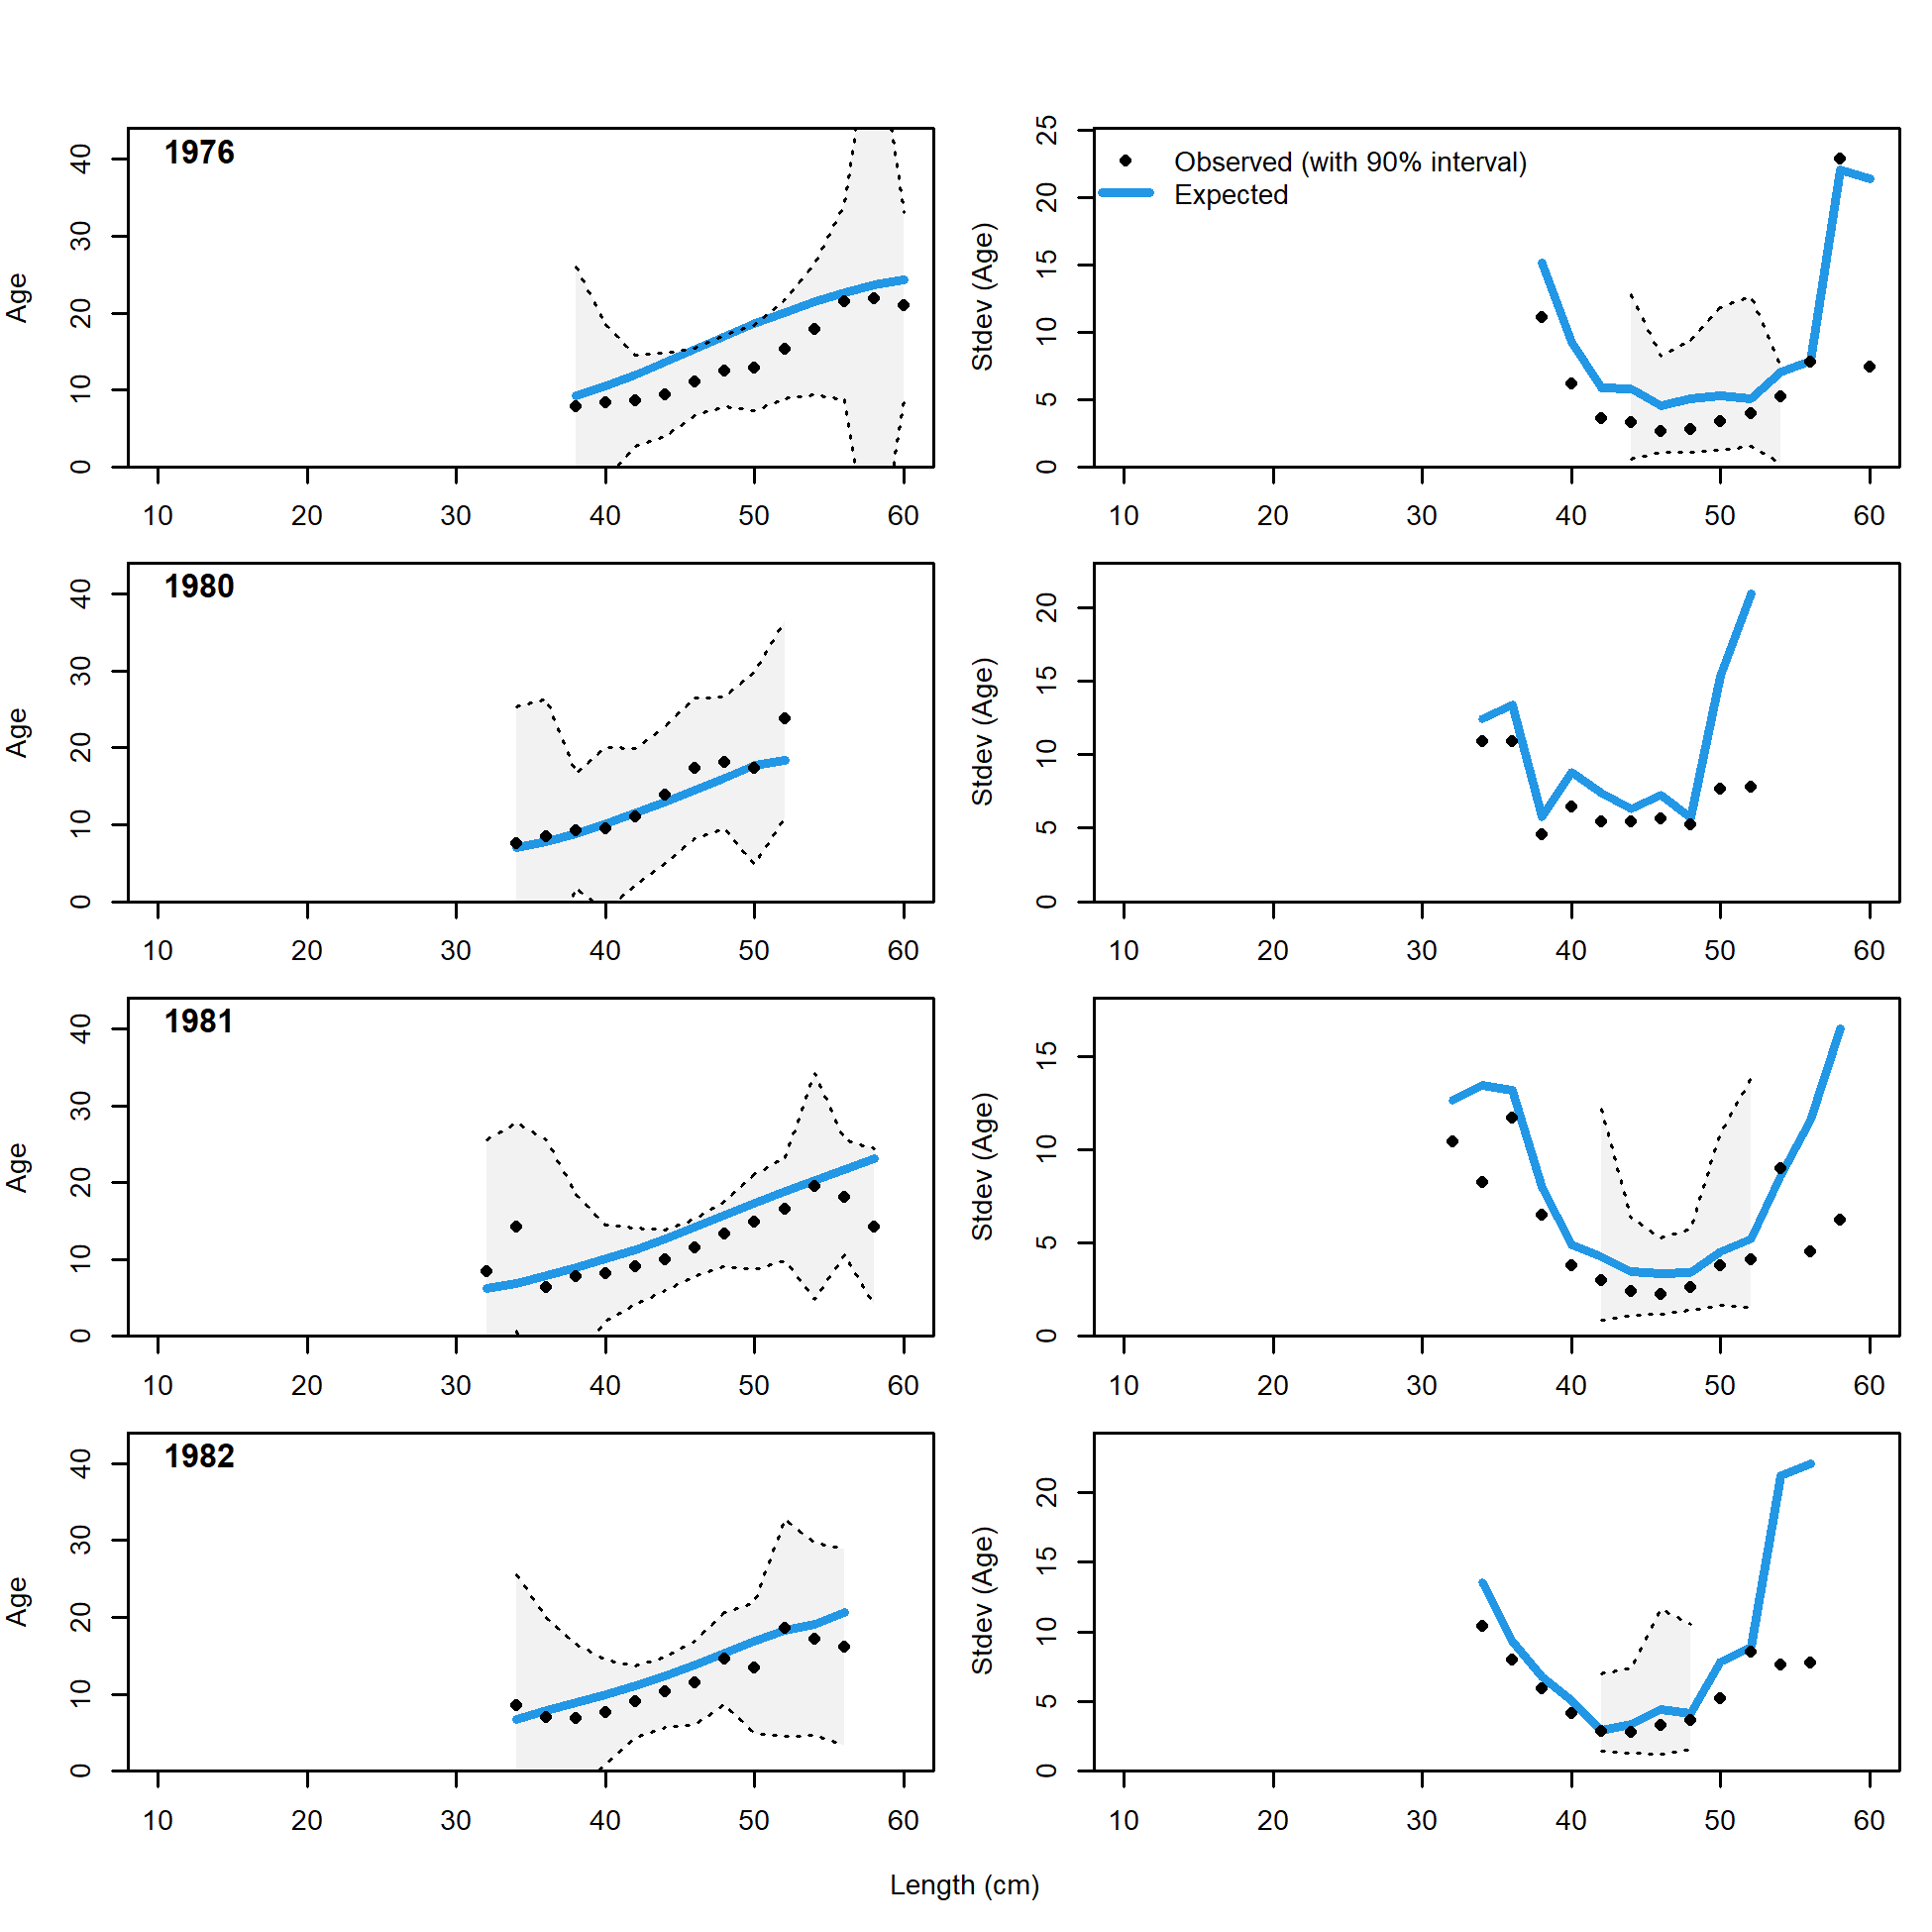
\includegraphics[width=1\textwidth,height=1\textheight]{C:/Users/Jason.Cope/Documents/Github/Sebastes_melanops_WA/Document/models/Reference model/plots/comp_condAALfit_Andre_plotsflt1mkt0_page1.png}
\caption{Trawl fishery conditional AAL plot (plot 1 of 5) showing mean age (left panel) and standard deviation (right panel. Shaded areas are 90 percent CIs).\label{fig:comp_condAALfit_Andre_plotsflt1mkt0_page1}}
\end{figure}

\begin{figure}
\centering
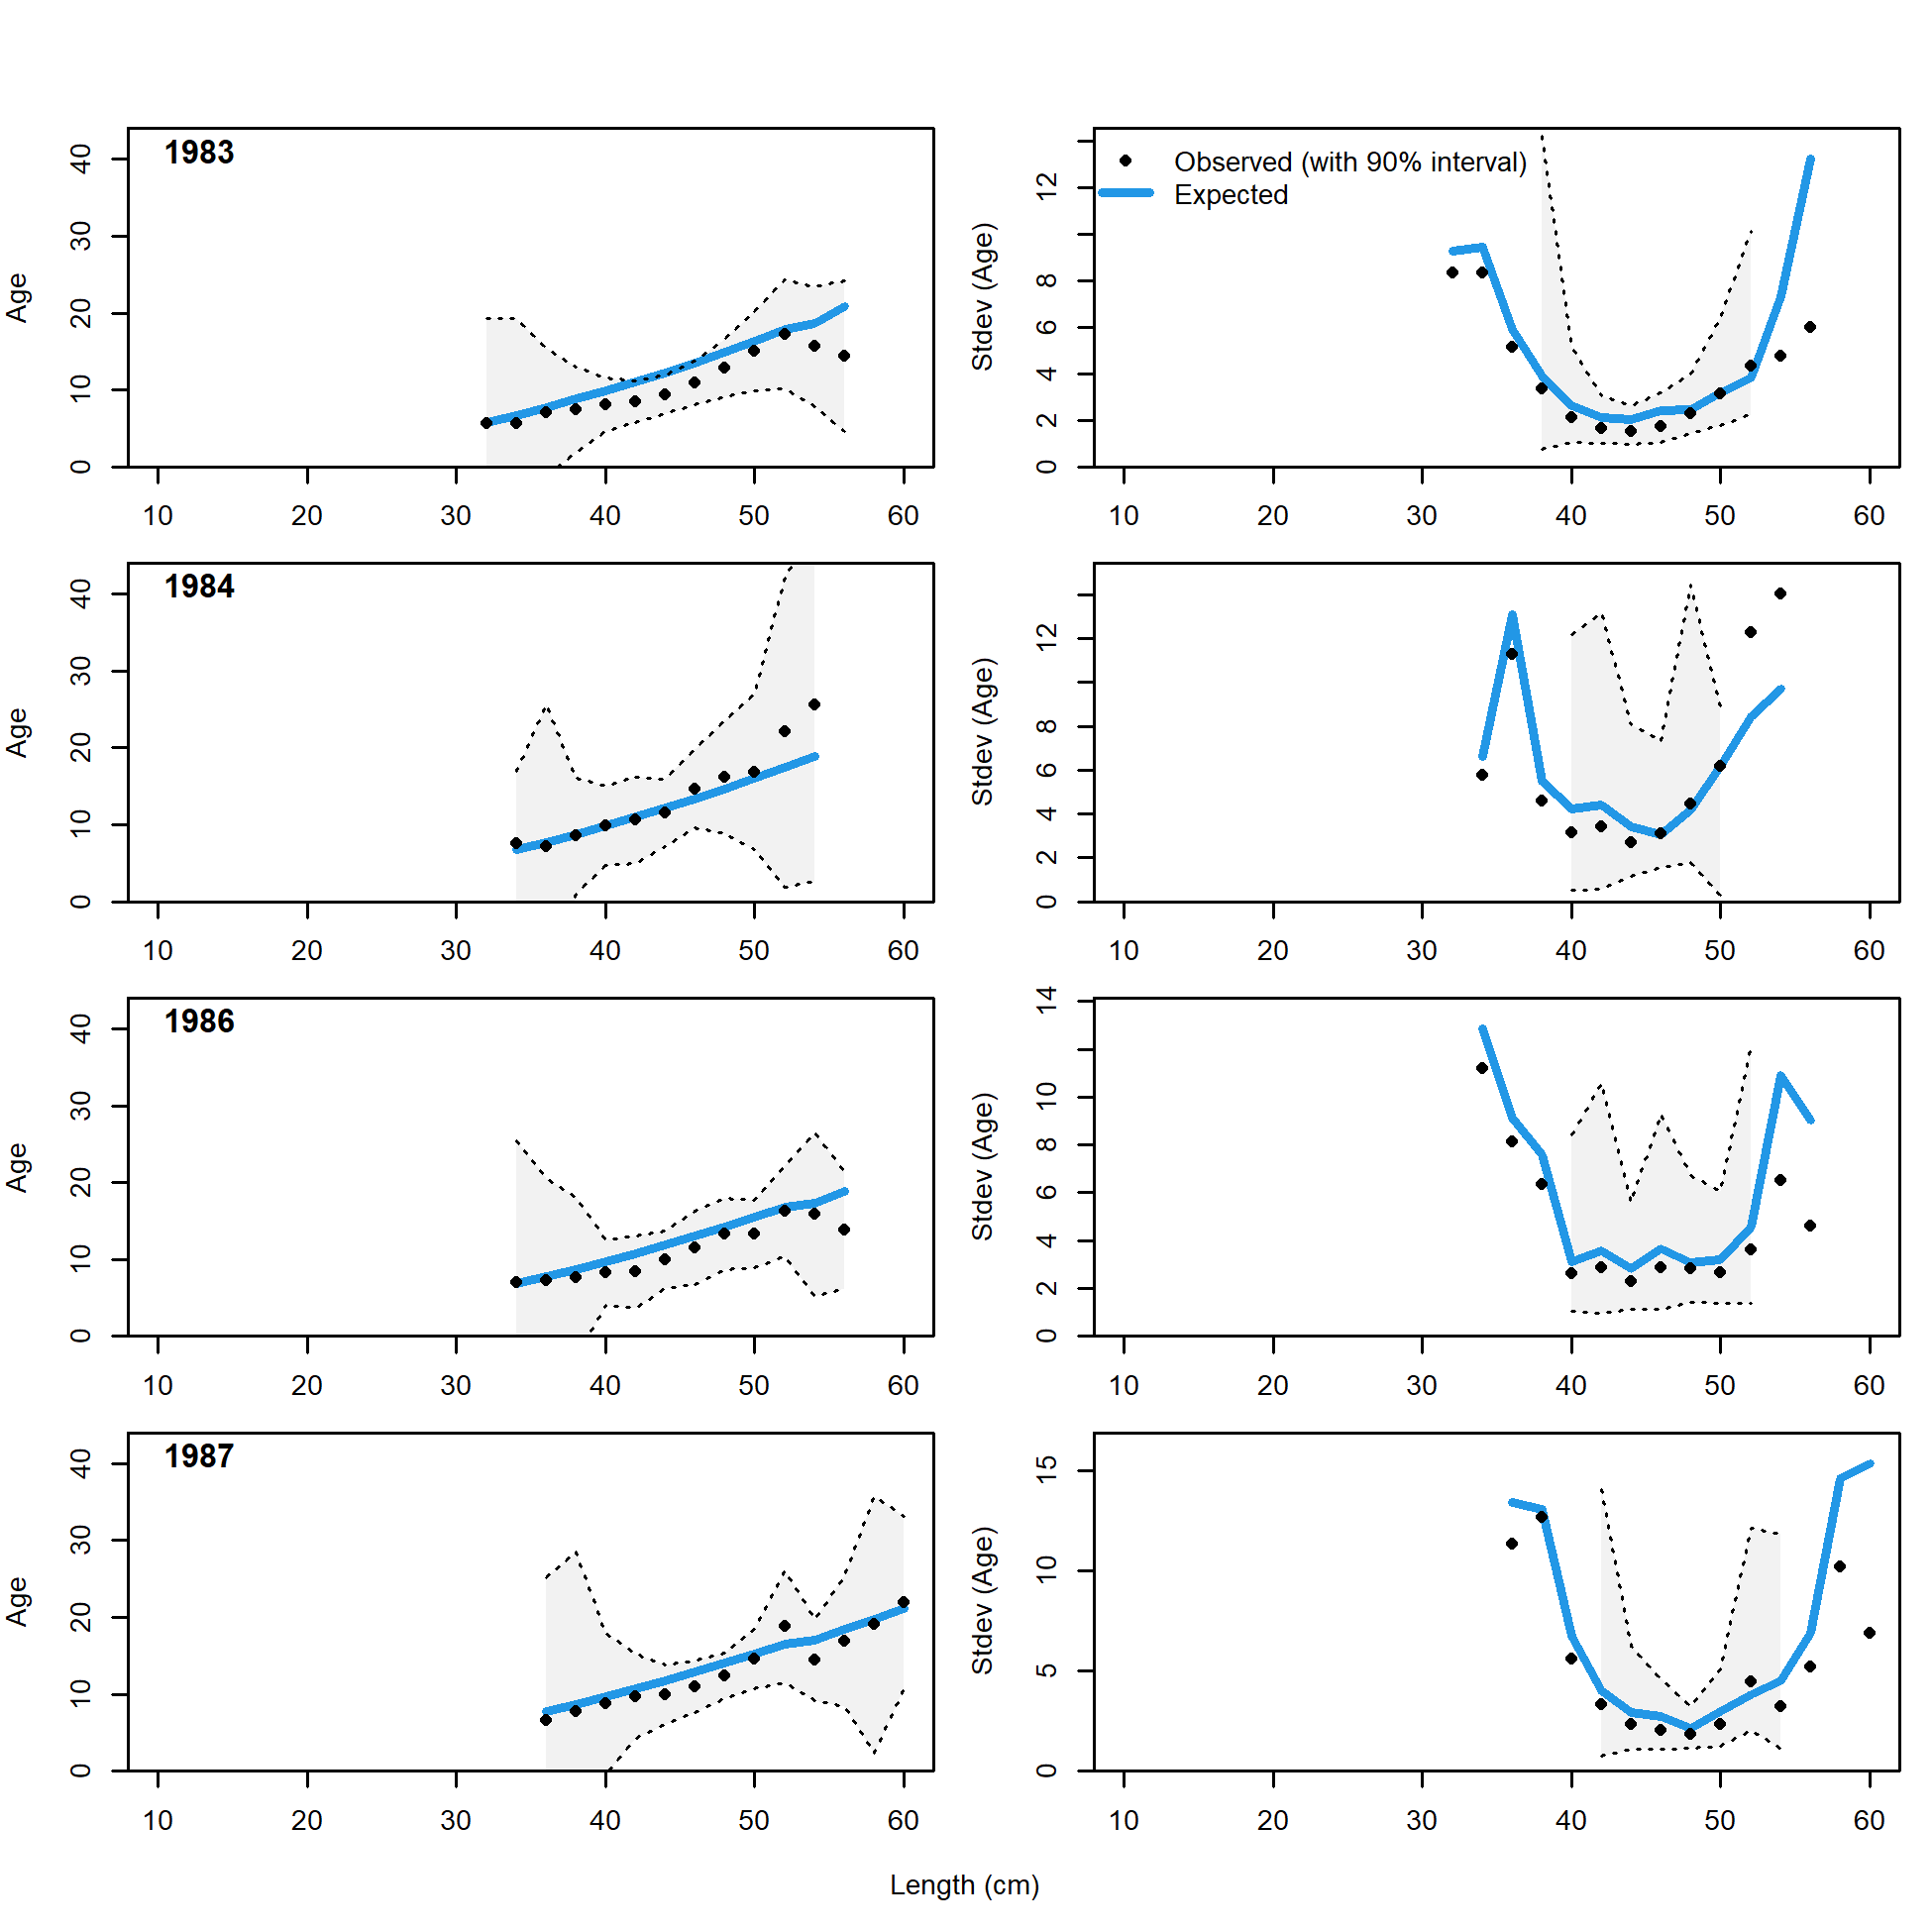
\includegraphics[width=1\textwidth,height=1\textheight]{C:/Users/Jason.Cope/Documents/Github/Sebastes_melanops_WA/Document/models/Reference model/plots/comp_condAALfit_Andre_plotsflt1mkt0_page2.png}
\caption{Trawl conditional AAL plot (plot 2 of 5).\label{fig:comp_condAALfit_Andre_plotsflt1mkt0_page2}}
\end{figure}

\begin{figure}
\centering
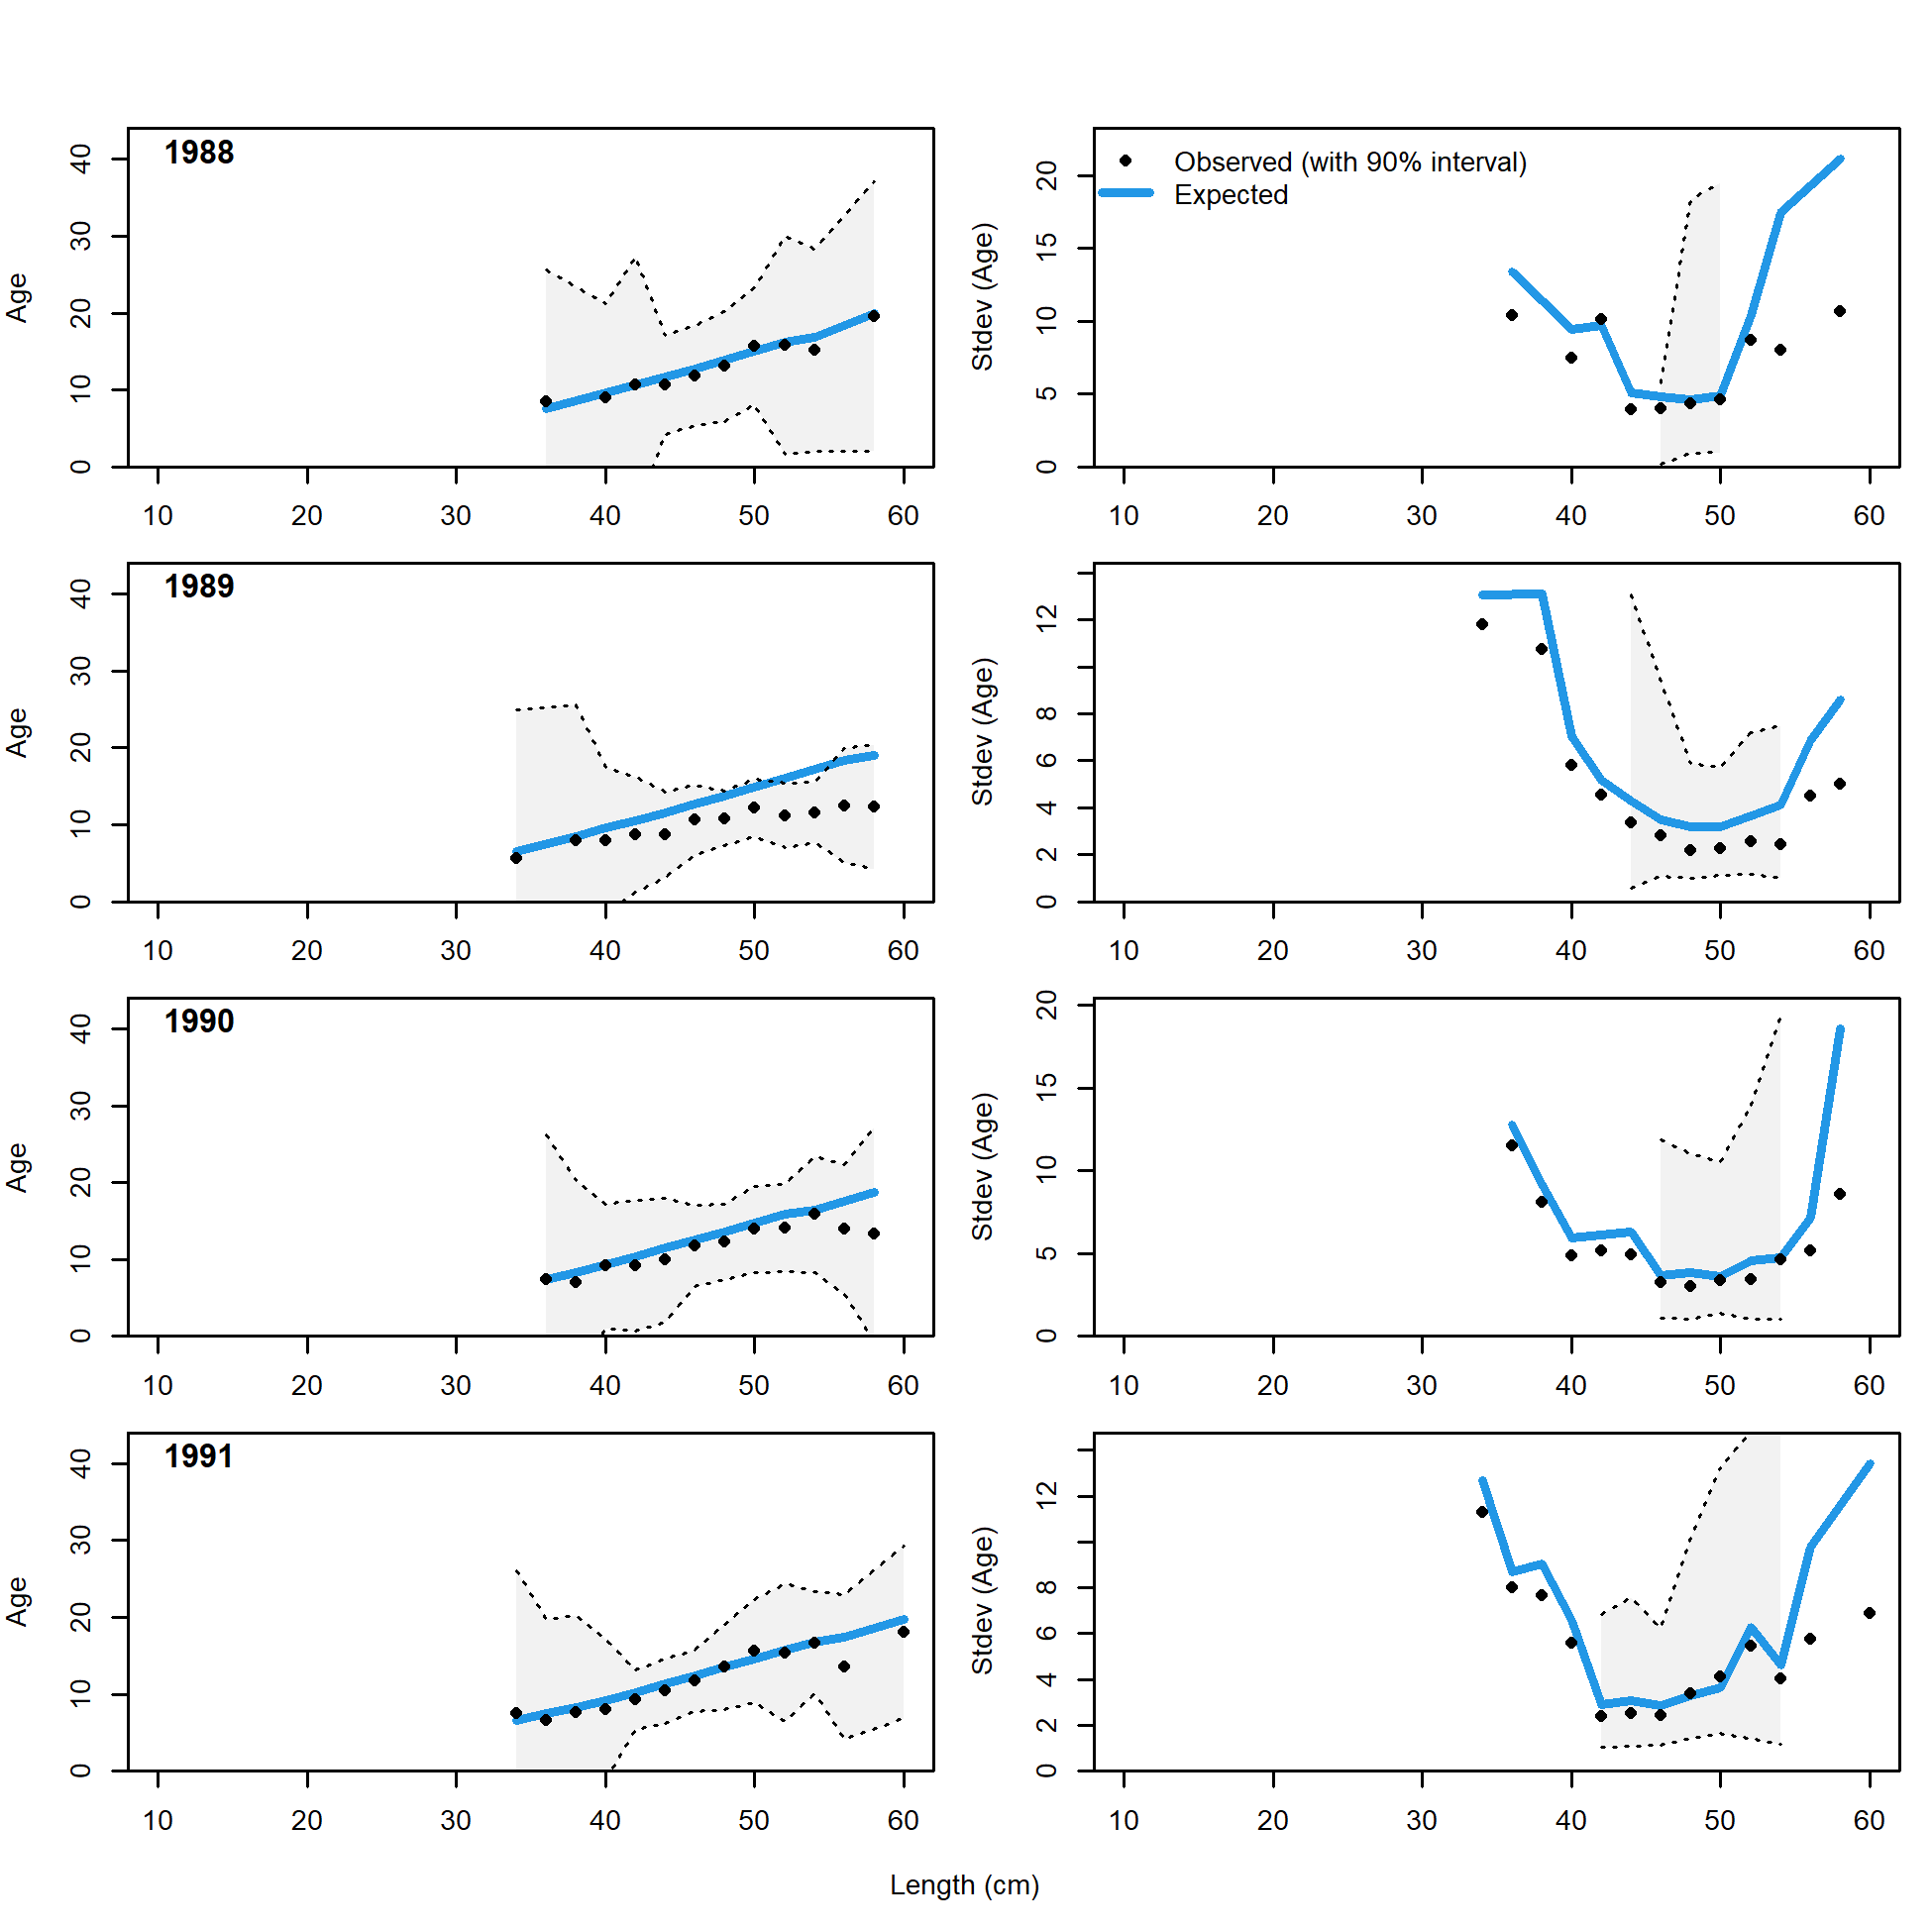
\includegraphics[width=1\textwidth,height=1\textheight]{C:/Users/Jason.Cope/Documents/Github/Sebastes_melanops_WA/Document/models/Reference model/plots/comp_condAALfit_Andre_plotsflt1mkt0_page3.png}
\caption{Trawl conditional AAL plot (plot 3 of 5).\label{fig:comp_condAALfit_Andre_plotsflt1mkt0_page3}}
\end{figure}

\begin{figure}
\centering
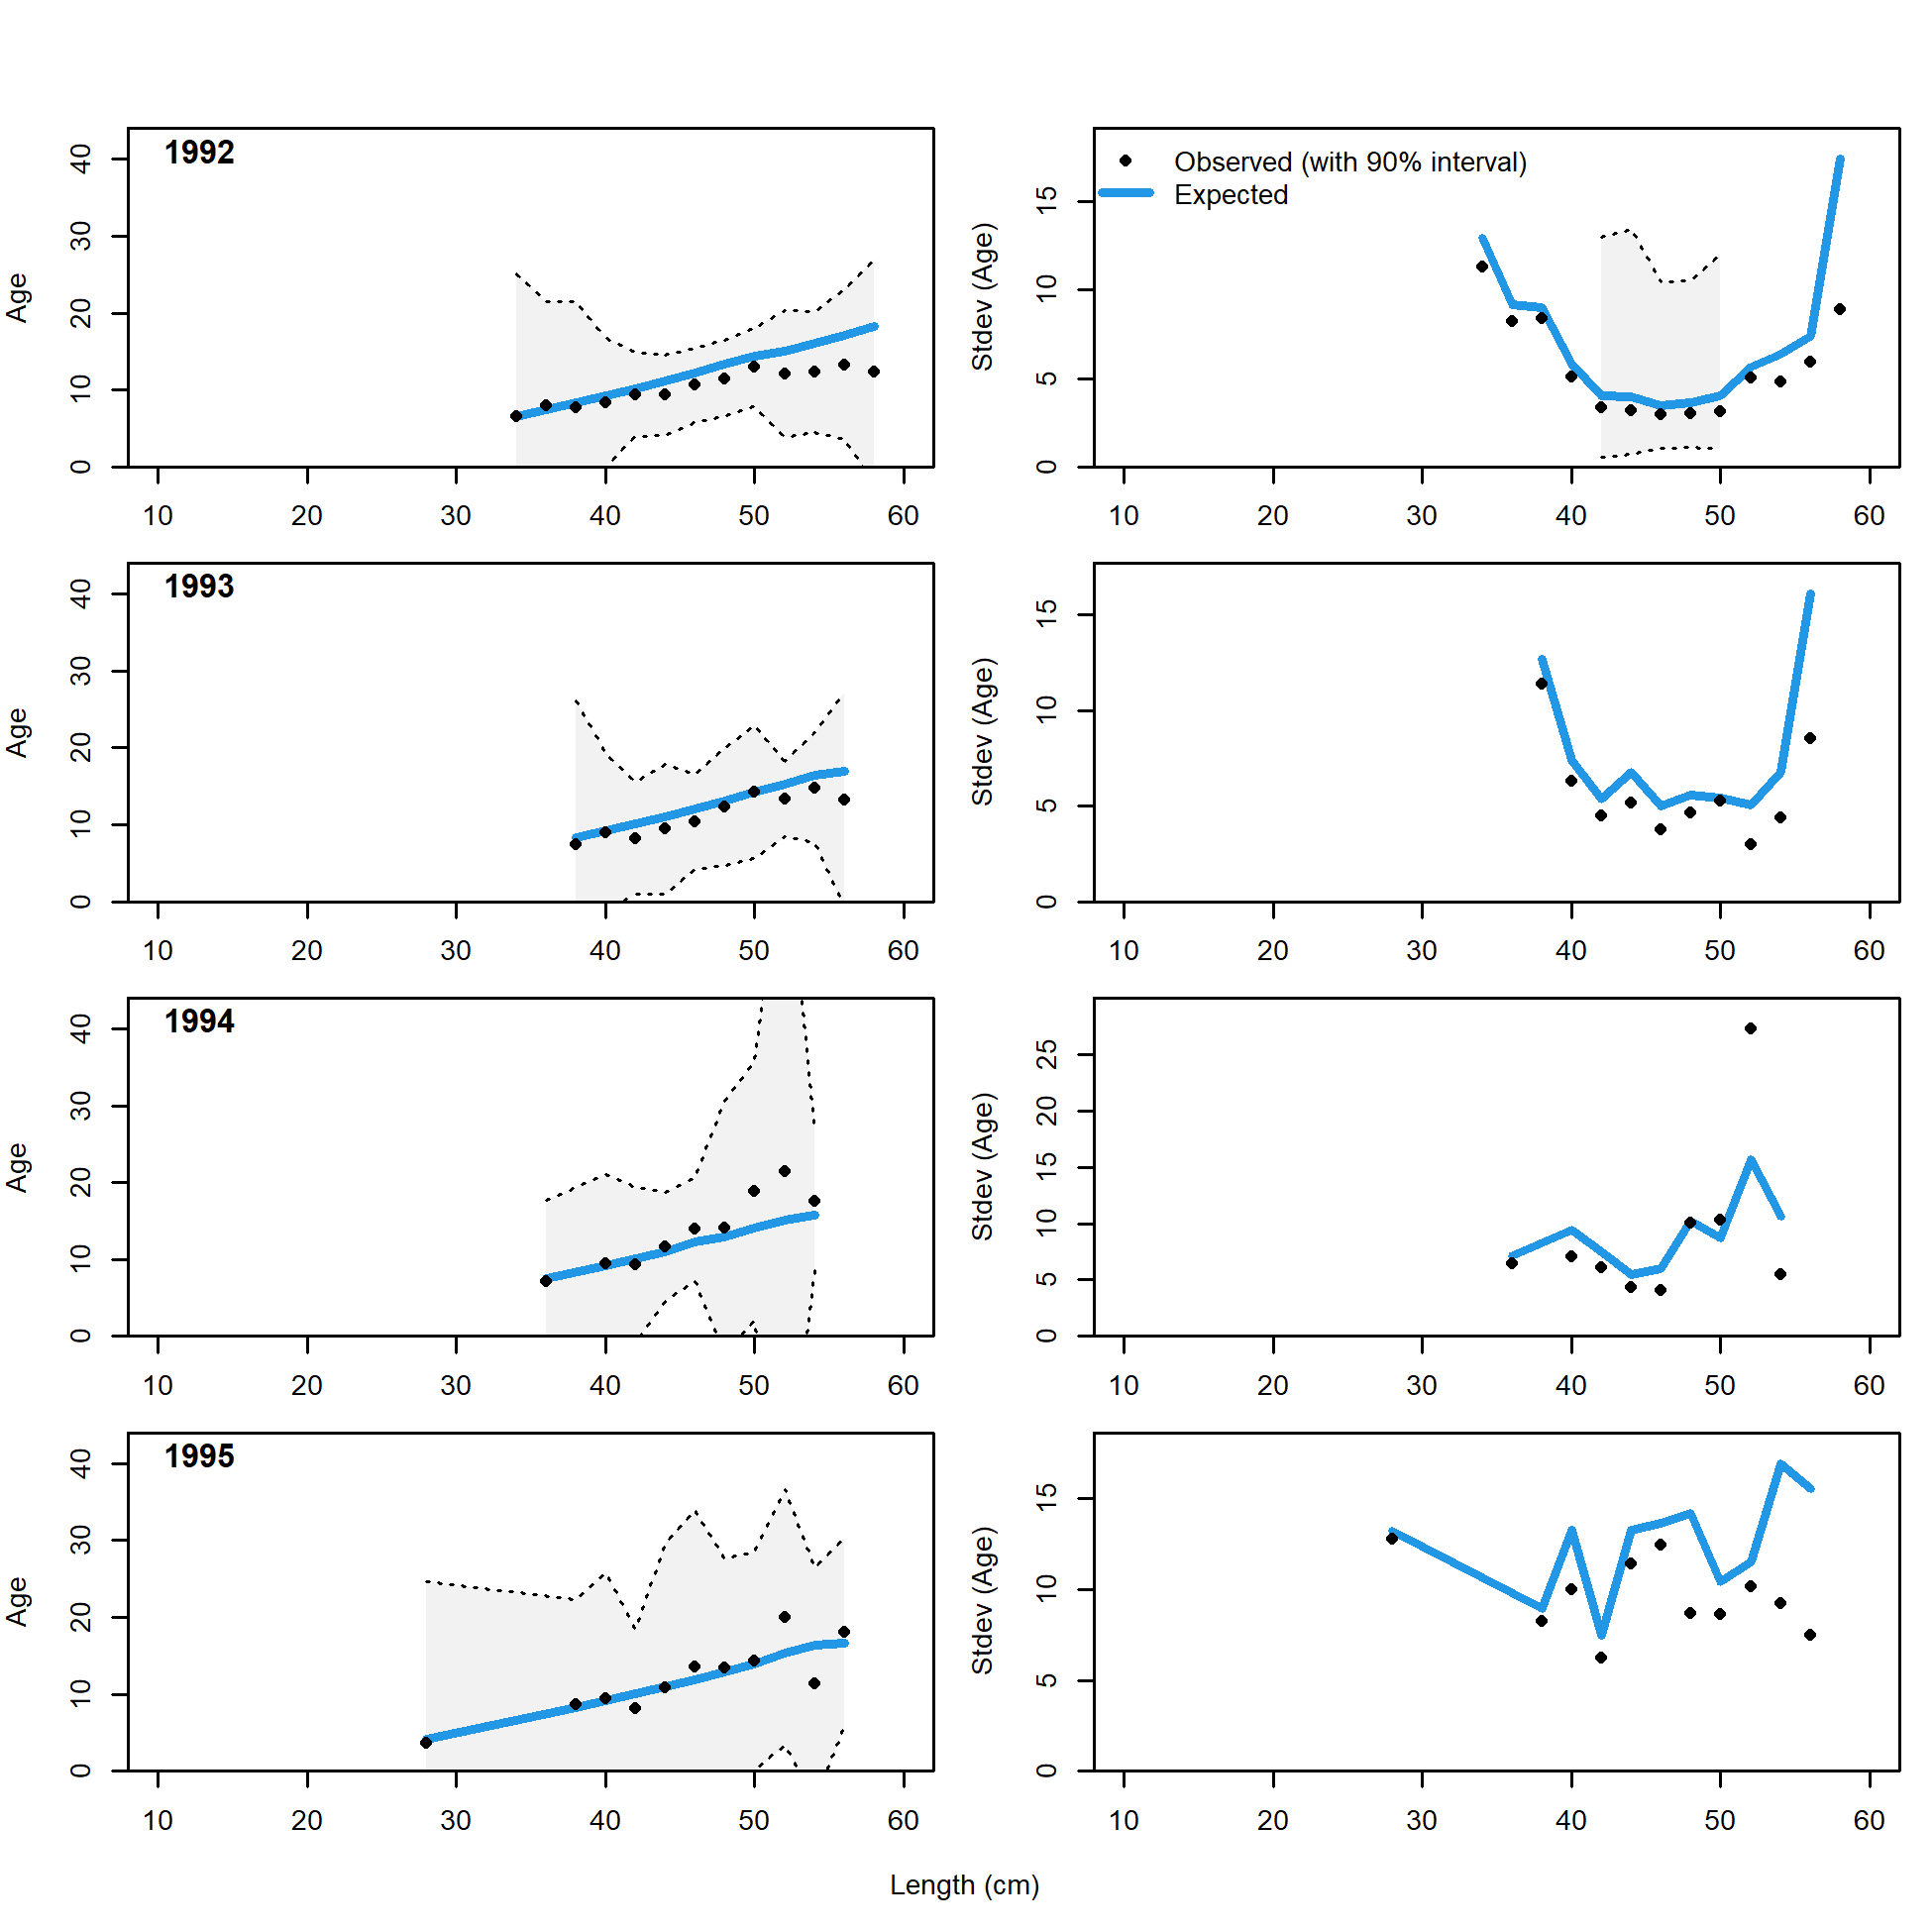
\includegraphics[width=1\textwidth,height=1\textheight]{C:/Users/Jason.Cope/Documents/Github/Sebastes_melanops_WA/Document/models/Reference model/plots/comp_condAALfit_Andre_plotsflt1mkt0_page4.png}
\caption{Trawl conditional AAL plot (plot 4 of 5).\label{fig:comp_condAALfit_Andre_plotsflt1mkt0_page4}}
\end{figure}

\begin{figure}
\centering
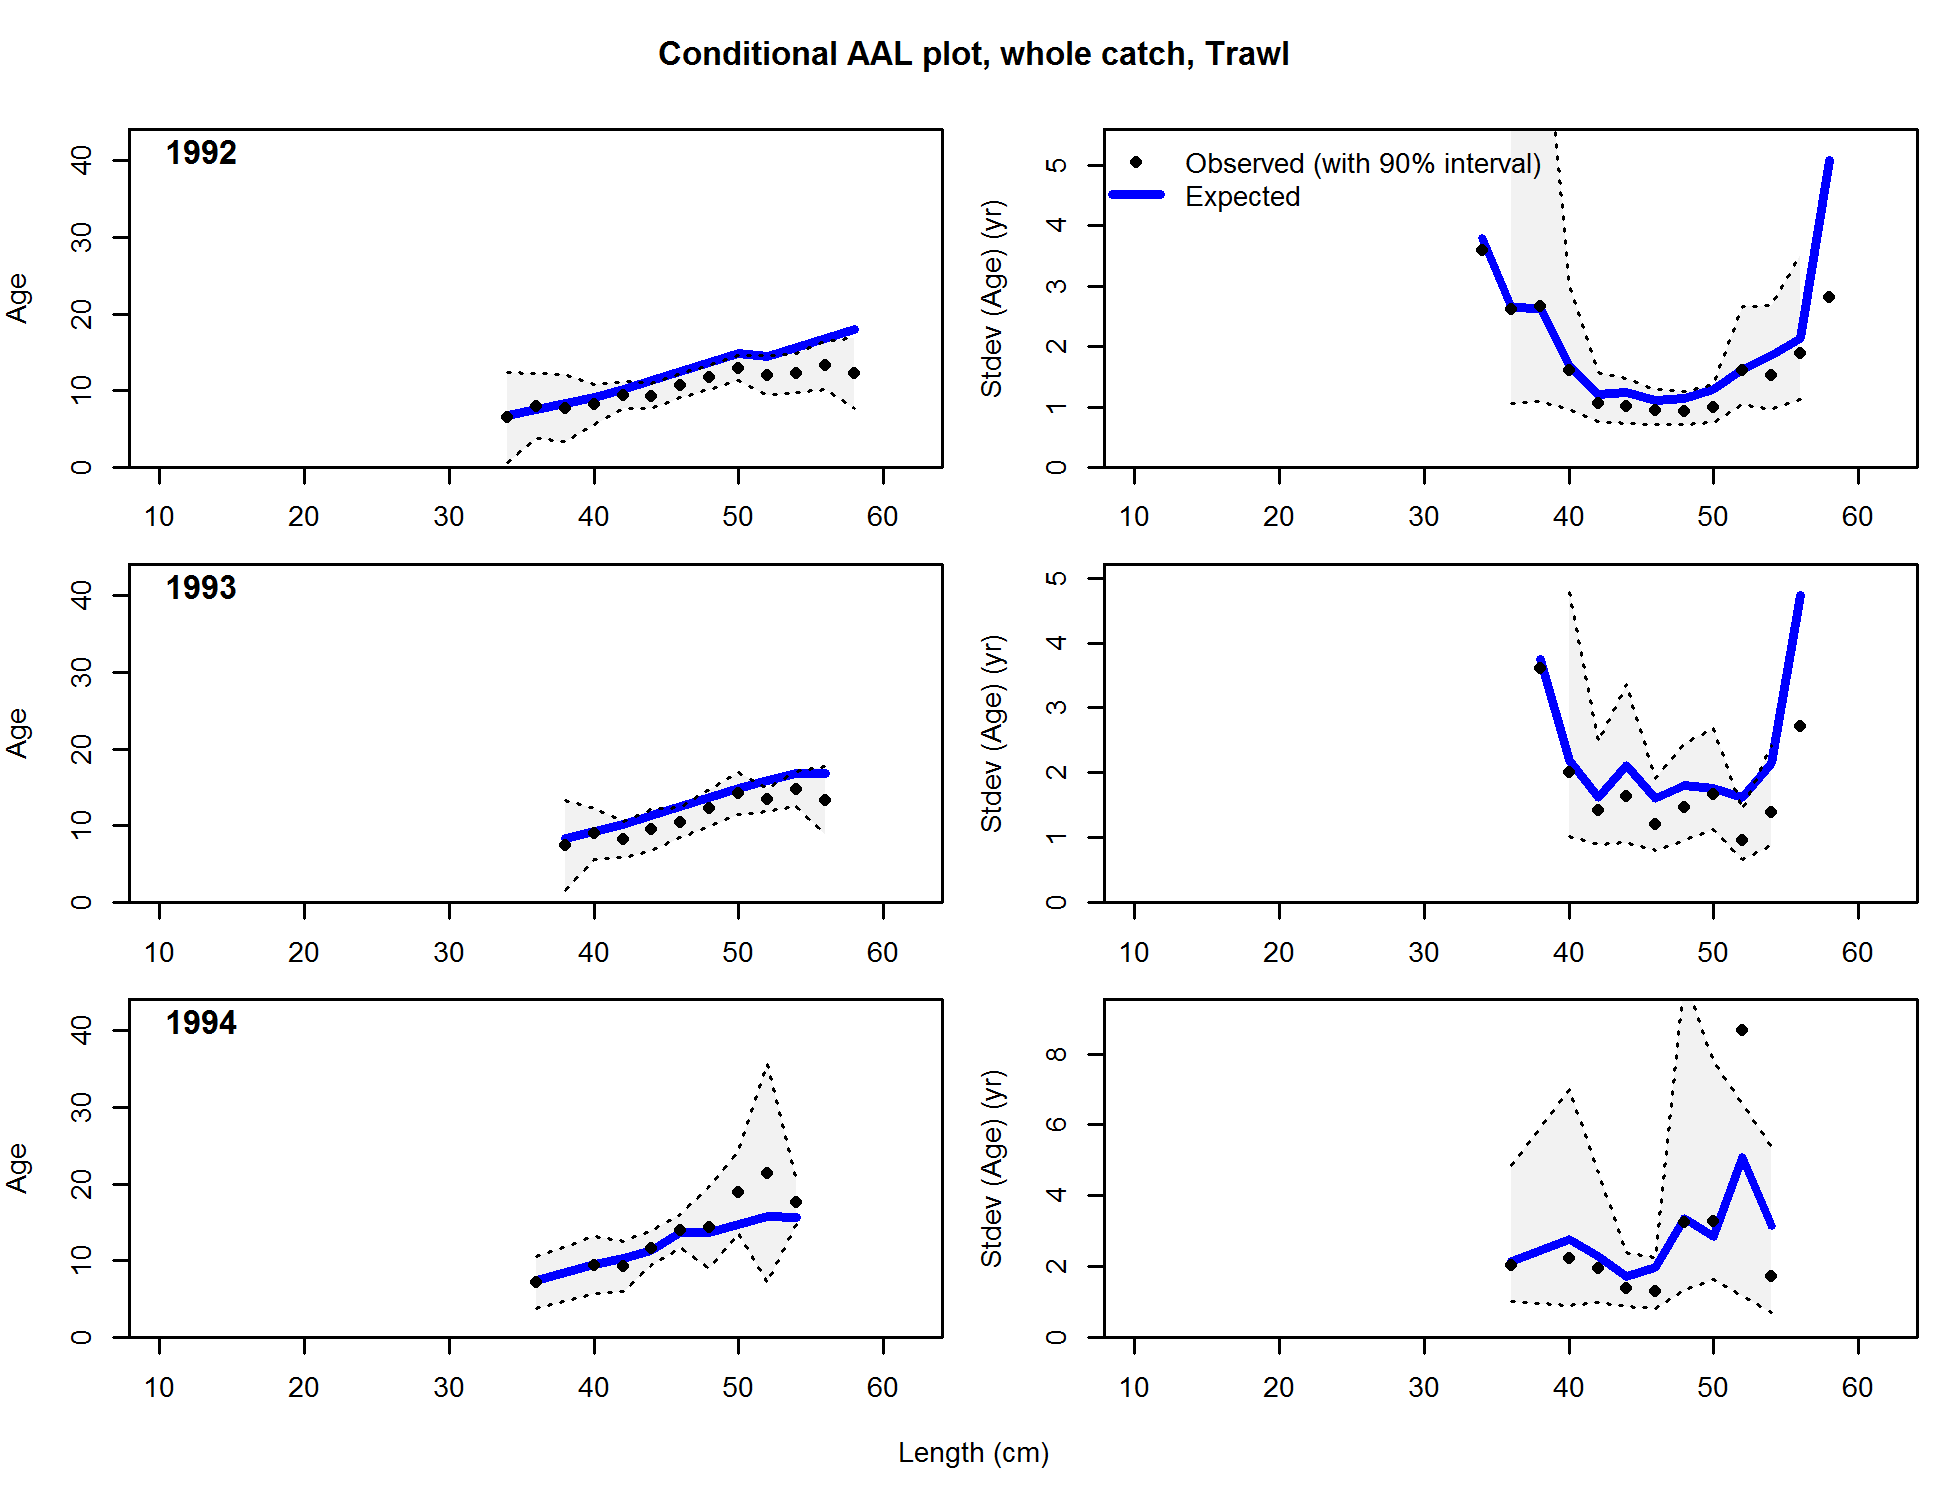
\includegraphics[width=1\textwidth,height=1\textheight]{C:/Users/Jason.Cope/Documents/Github/Sebastes_melanops_WA/Document/models/Reference model/plots/comp_condAALfit_Andre_plotsflt1mkt0_page5.png}
\caption{Trawl conditional AAL plot (plot 5 of 5).\label{fig:comp_condAALfit_Andre_plotsflt1mkt0_page5}}
\end{figure}

\begin{figure}
\centering
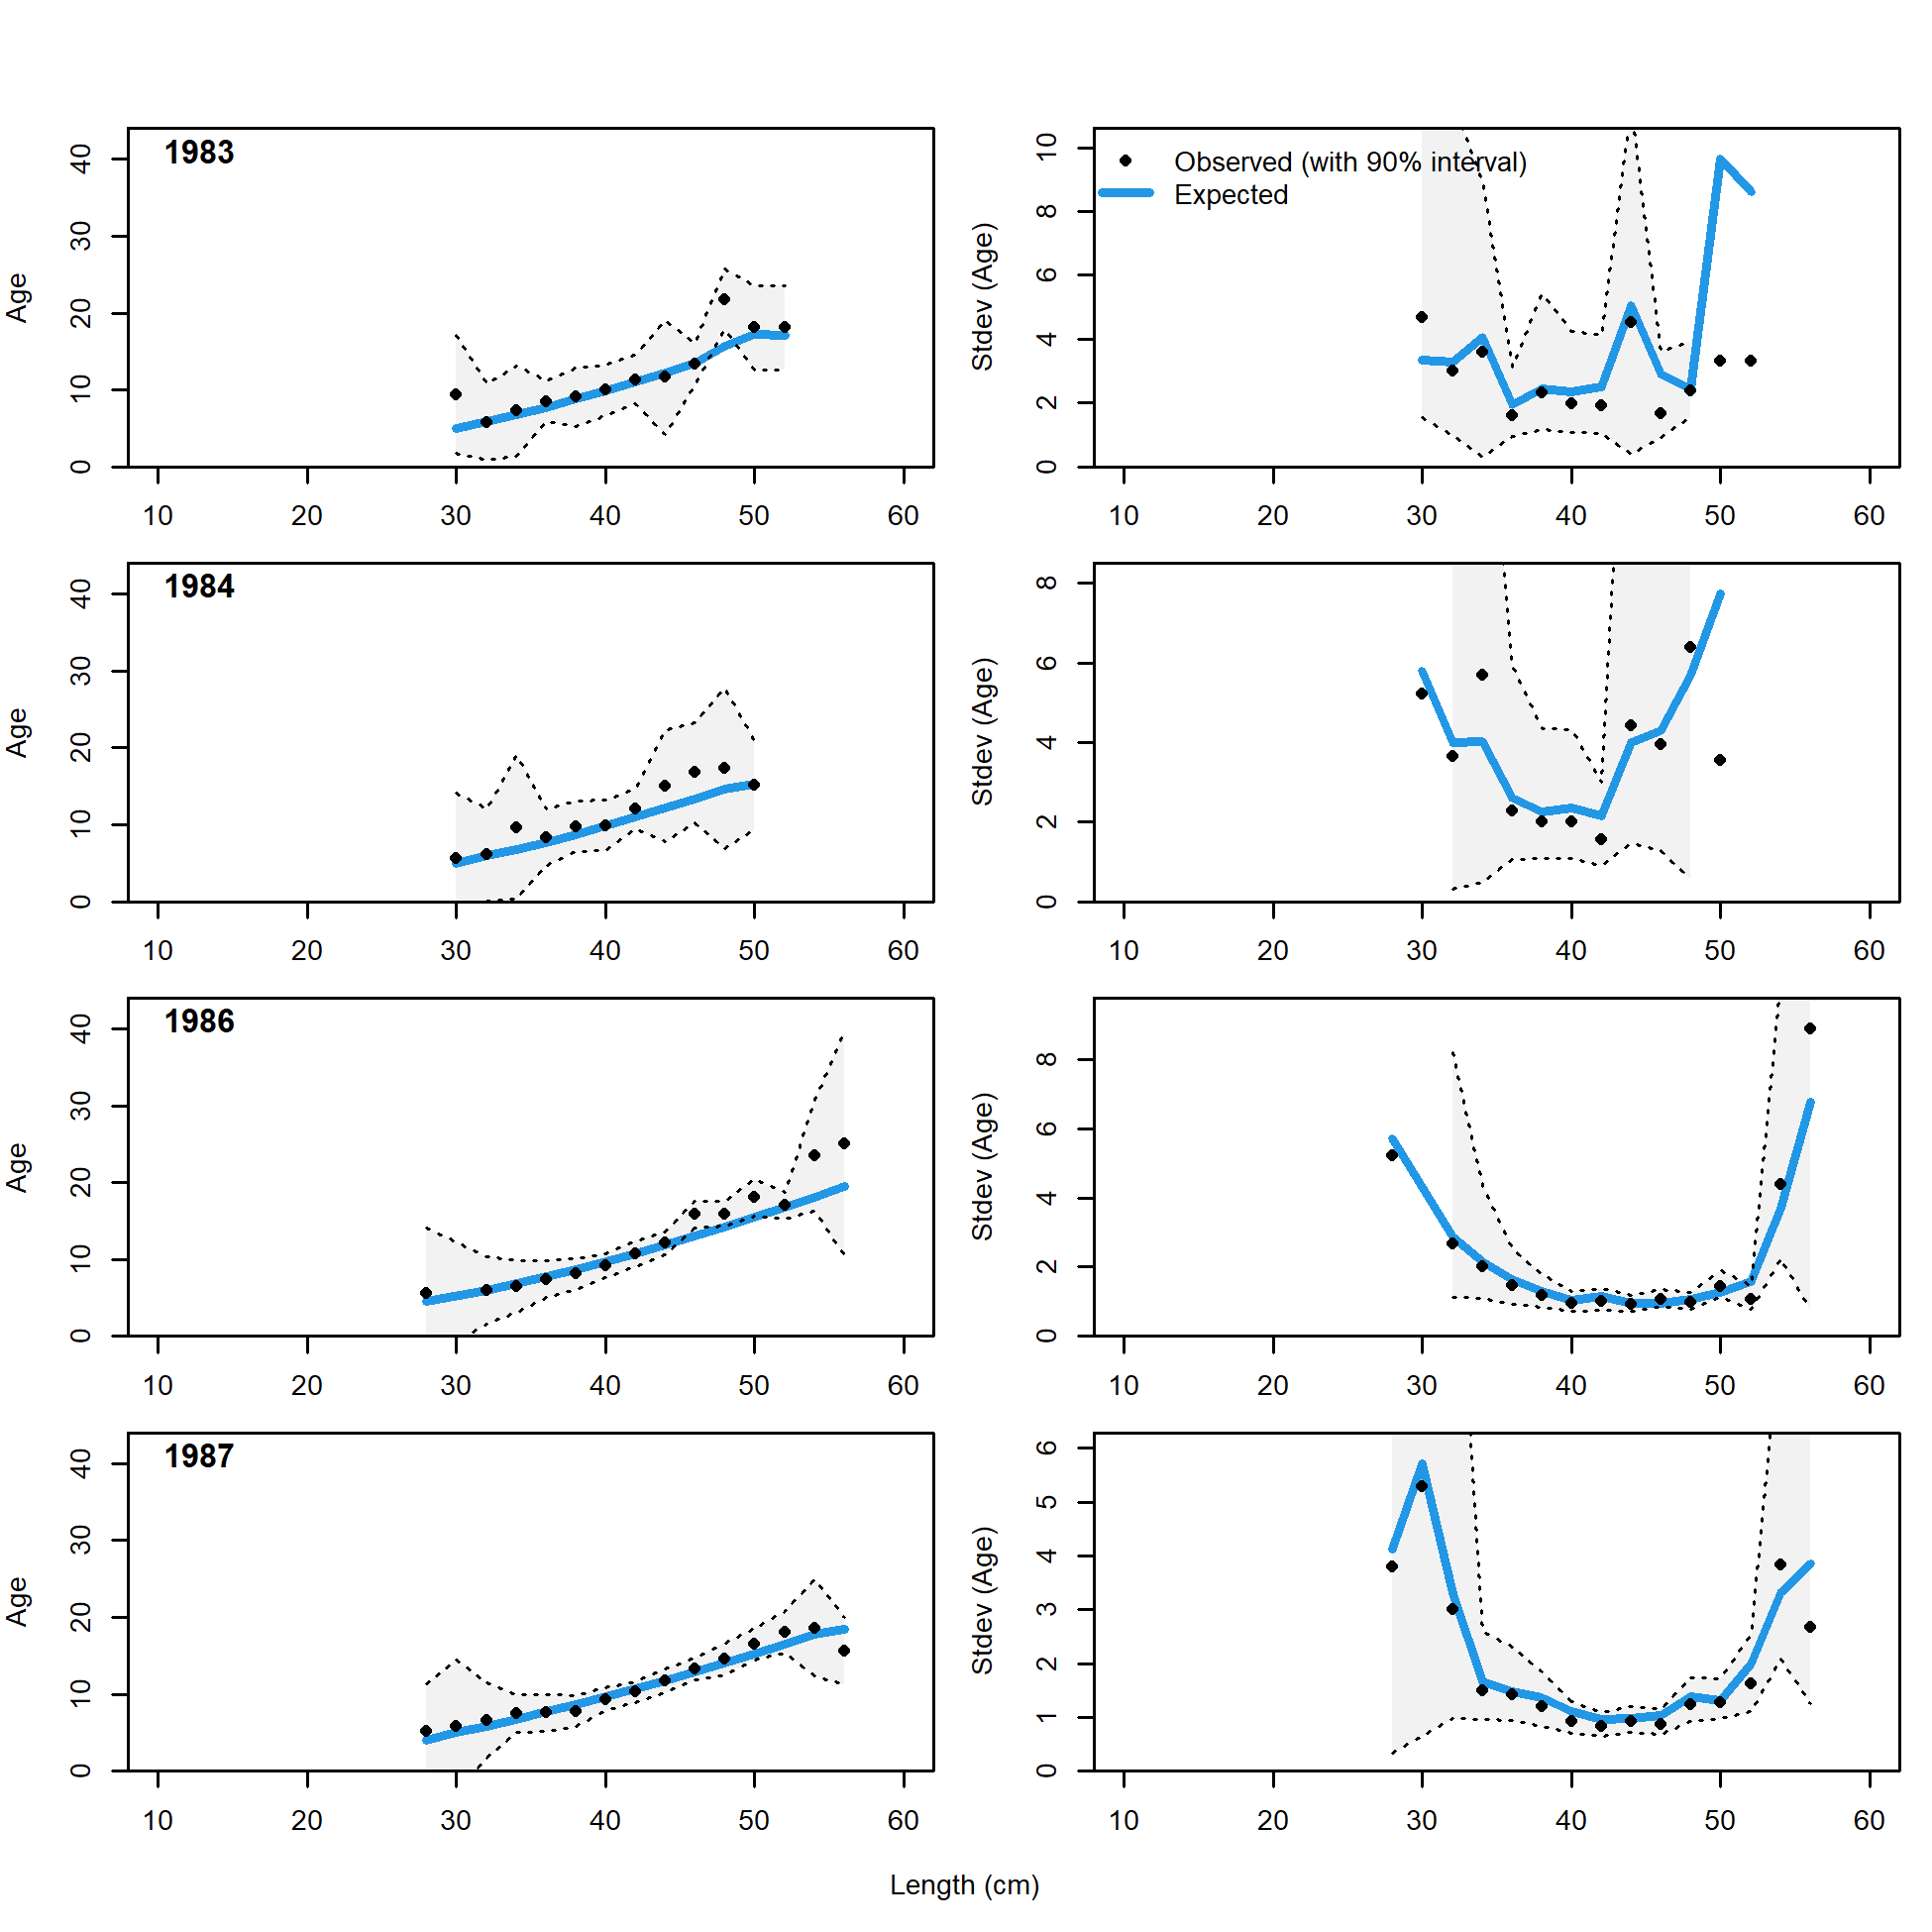
\includegraphics[width=1\textwidth,height=1\textheight]{C:/Users/Jason.Cope/Documents/Github/Sebastes_melanops_WA/Document/models/Reference model/plots/comp_condAALfit_Andre_plotsflt2mkt0_page1.png}
\caption{Non-trawl (jig) fishery conditional AAL plot (plot 1 of 2) showing mean age (left panel) and standard deviation (right panel. Shaded areas are 90 percent CIs).\label{fig:comp_condAALfit_Andre_plotsflt2mkt0_page1}}
\end{figure}

\begin{figure}
\centering
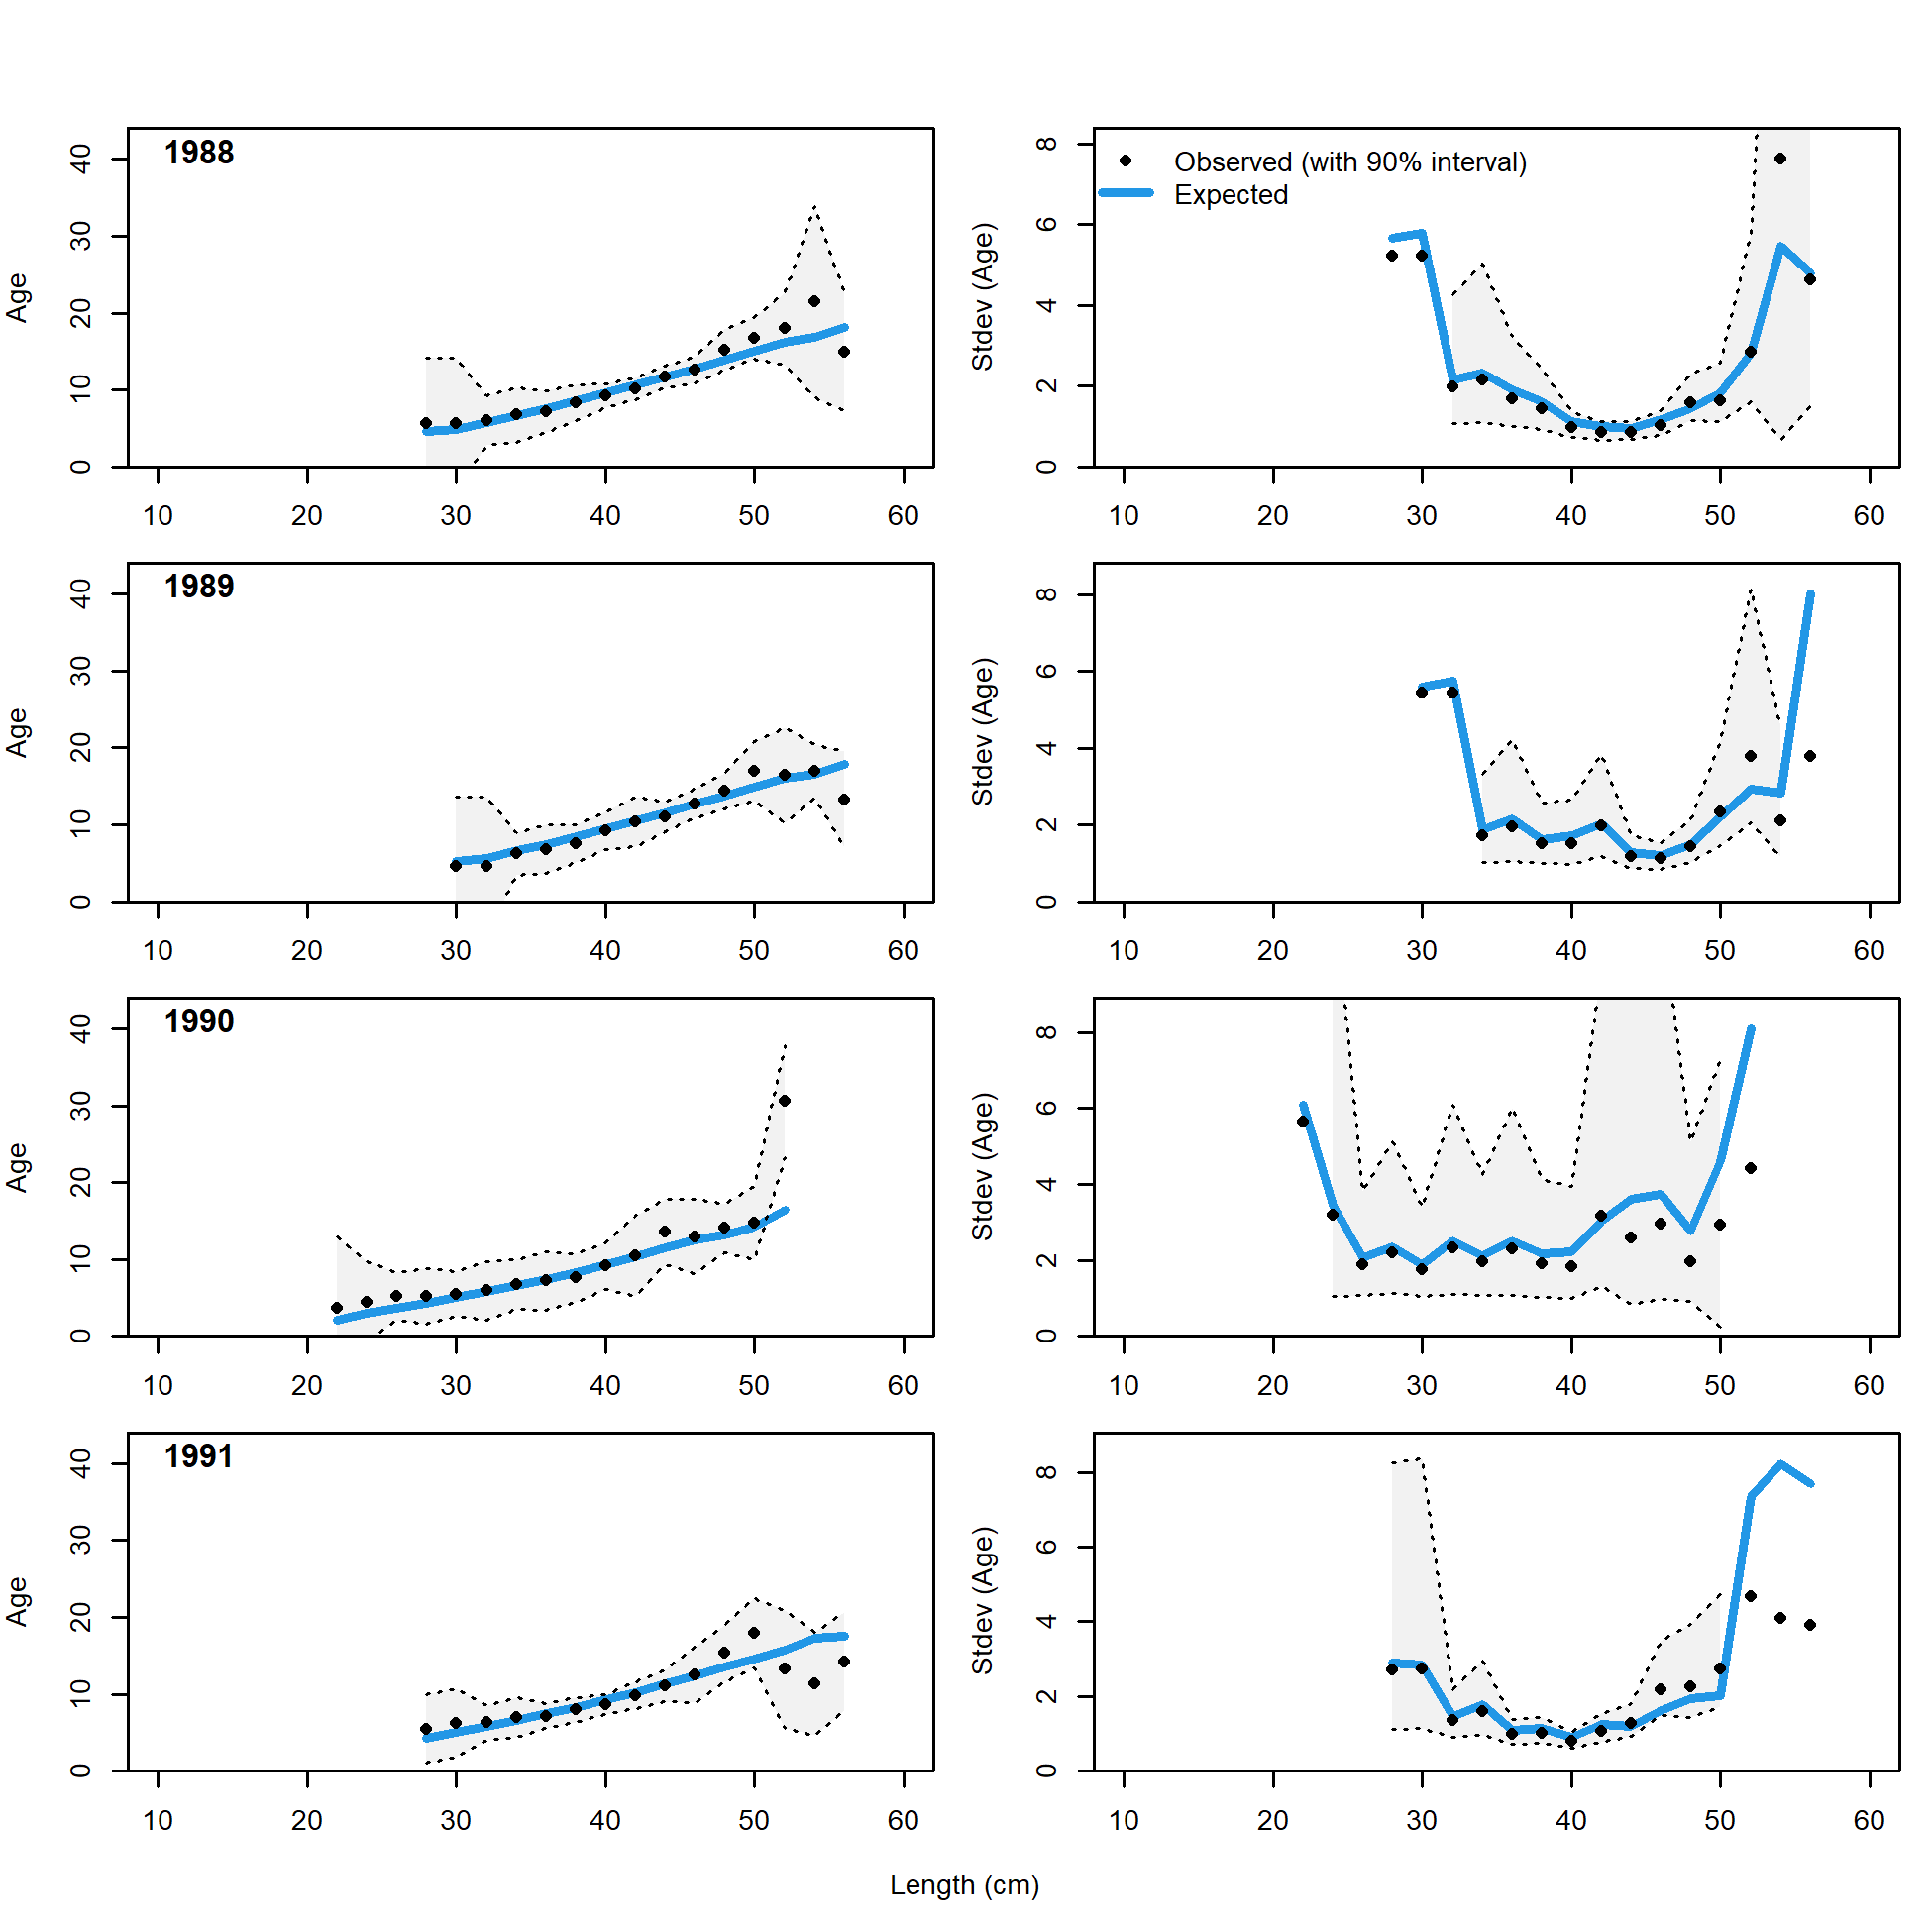
\includegraphics[width=1\textwidth,height=1\textheight]{C:/Users/Jason.Cope/Documents/Github/Sebastes_melanops_WA/Document/models/Reference model/plots/comp_condAALfit_Andre_plotsflt2mkt0_page2.png}
\caption{Non-trawl (jig) conditional AAL plot (plot 2 of 2).\label{fig:comp_condAALfit_Andre_plotsflt2mkt0_page2}}
\end{figure}

\begin{figure}
\centering
\includegraphics[width=1\textwidth,height=1\textheight]{C:/Users/Jason.Cope/Documents/Github/Sebastes_melanops_WA/Document/models/Reference model/plots/comp_condAALfit_Andre_plotsflt2mkt0_page3.png}
\caption{Non-trawl (jig) conditional AAL plot (plot 3 of 3).\label{fig:comp_condAALfit_Andre_plotsflt2mkt0_page3}}
\end{figure}

\begin{figure}
\centering
\includegraphics[width=1\textwidth,height=1\textheight]{C:/Users/Jason.Cope/Documents/Github/Sebastes_melanops_WA/Document/models/Reference model/plots/comp_condAALfit_Andre_plotsflt3mkt0_page1.png}
\caption{Ocean boat conditional AAL plot (plot 1 of 11) showing mean age (left panel) and standard deviation (right panel. Shaded areas are 90 percent CIs).\label{fig:comp_condAALfit_Andre_plotsflt3mkt0_page1}}
\end{figure}

\begin{figure}
\centering
\includegraphics[width=1\textwidth,height=1\textheight]{C:/Users/Jason.Cope/Documents/Github/Sebastes_melanops_WA/Document/models/Reference model/plots/comp_condAALfit_Andre_plotsflt3mkt0_page10.png}
\caption{Ocean boat conditional AAL plot (plot 2 of 11).\label{fig:comp_condAALfit_Andre_plotsflt3mkt0_page10}}
\end{figure}

\begin{figure}
\centering
\includegraphics[width=1\textwidth,height=1\textheight]{C:/Users/Jason.Cope/Documents/Github/Sebastes_melanops_WA/Document/models/Reference model/plots/comp_condAALfit_Andre_plotsflt3mkt0_page11.png}
\caption{Ocean boat conditional AAL plot (plot 3 of 11).\label{fig:comp_condAALfit_Andre_plotsflt3mkt0_page11}}
\end{figure}

\begin{figure}
\centering
\includegraphics[width=1\textwidth,height=1\textheight]{C:/Users/Jason.Cope/Documents/Github/Sebastes_melanops_WA/Document/models/Reference model/plots/comp_condAALfit_Andre_plotsflt3mkt0_page2.png}
\caption{Ocean boat conditional AAL plot (plot 3 of 11).\label{fig:comp_condAALfit_Andre_plotsflt3mkt0_page2}}
\end{figure}

\begin{figure}
\centering
\includegraphics[width=1\textwidth,height=1\textheight]{C:/Users/Jason.Cope/Documents/Github/Sebastes_melanops_WA/Document/models/Reference model/plots/comp_condAALfit_Andre_plotsflt3mkt0_page3.png}
\caption{Ocean boat conditional AAL plot (plot 4 of 11).\label{fig:comp_condAALfit_Andre_plotsflt3mkt0_page3}}
\end{figure}

\begin{figure}
\centering
\includegraphics[width=1\textwidth,height=1\textheight]{C:/Users/Jason.Cope/Documents/Github/Sebastes_melanops_WA/Document/models/Reference model/plots/comp_condAALfit_Andre_plotsflt3mkt0_page4.png}
\caption{Ocean boat conditional AAL plot (plot 5 of 11).\label{fig:comp_condAALfit_Andre_plotsflt3mkt0_page4}}
\end{figure}

\begin{figure}
\centering
\includegraphics[width=1\textwidth,height=1\textheight]{C:/Users/Jason.Cope/Documents/Github/Sebastes_melanops_WA/Document/models/Reference model/plots/comp_condAALfit_Andre_plotsflt3mkt0_page5.png}
\caption{Ocean boat conditional AAL plot (plot 6 of 11).\label{fig:comp_condAALfit_Andre_plotsflt3mkt0_page5}}
\end{figure}

\begin{figure}
\centering
\includegraphics[width=1\textwidth,height=1\textheight]{C:/Users/Jason.Cope/Documents/Github/Sebastes_melanops_WA/Document/models/Reference model/plots/comp_condAALfit_Andre_plotsflt3mkt0_page6.png}
\caption{Ocean boat conditional AAL plot (plot 7 of 11).\label{fig:comp_condAALfit_Andre_plotsflt3mkt0_page6}}
\end{figure}

\begin{figure}
\centering
\includegraphics[width=1\textwidth,height=1\textheight]{C:/Users/Jason.Cope/Documents/Github/Sebastes_melanops_WA/Document/models/Reference model/plots/comp_condAALfit_Andre_plotsflt3mkt0_page7.png}
\caption{Ocean boat conditional AAL plot (plot 8 of 11).\label{fig:comp_condAALfit_Andre_plotsflt3mkt0_page7}}
\end{figure}

\begin{figure}
\centering
\includegraphics[width=1\textwidth,height=1\textheight]{C:/Users/Jason.Cope/Documents/Github/Sebastes_melanops_WA/Document/models/Reference model/plots/comp_condAALfit_Andre_plotsflt3mkt0_page8.png}
\caption{Ocean boat conditional AAL plot (plot 9 of 11).\label{fig:comp_condAALfit_Andre_plotsflt3mkt0_page8}}
\end{figure}

\begin{figure}
\centering
\includegraphics[width=1\textwidth,height=1\textheight]{C:/Users/Jason.Cope/Documents/Github/Sebastes_melanops_WA/Document/models/Reference model/plots/comp_condAALfit_Andre_plotsflt3mkt0_page9.png}
\caption{Ocean boat conditional AAL plot (plot 10 of 11).\label{fig:comp_condAALfit_Andre_plotsflt3mkt0_page9}}
\end{figure}

\clearpage

\hypertarget{app-d}{%
\section{Appendix D: Passive Fit to Marginal Age Composition Data}\label{app-d}}

\begin{figure}
\centering
\includegraphics[width=1\textwidth,height=1\textheight]{C:/Users/Jason.Cope/Documents/Github/Sebastes_melanops_WA/Document/models/Reference model/plots/comp_gstagefit_flt1mkt0.png}
\caption{Excluded age comps, whole catch, Trawl.`N adj.' is the input sample size after data-weighting adjustment. N eff. is the calculated effective sample size used in the McAllister-Ianelli tuning method.\label{fig:comp_gstagefit_flt1mkt0}}
\end{figure}

\begin{figure}
\centering
\includegraphics[width=1\textwidth,height=1\textheight]{C:/Users/Jason.Cope/Documents/Github/Sebastes_melanops_WA/Document/models/Reference model/plots/comp_gstagefit_flt2mkt0.png}
\caption{Excluded age comps, whole catch, NonTRWL.`N adj.' is the input sample size after data-weighting adjustment. N eff. is the calculated effective sample size used in the McAllister-Ianelli tuning method.\label{fig:comp_gstagefit_flt2mkt0}}
\end{figure}

\begin{figure}
\centering
\includegraphics[width=1\textwidth,height=1\textheight]{C:/Users/Jason.Cope/Documents/Github/Sebastes_melanops_WA/Document/models/Reference model/plots/comp_gstagefit_flt3mkt0_page1.png}
\caption{Excluded age comps, whole catch, Recreational (plot 1 of 2).`N adj.' is the input sample size after data-weighting adjustment. N eff. is the calculated effective sample size used in the McAllister-Ianelli tuning method.\label{fig:comp_gstagefit_flt3mkt0_page1}}
\end{figure}

\begin{figure}
\centering
\includegraphics[width=1\textwidth,height=1\textheight]{C:/Users/Jason.Cope/Documents/Github/Sebastes_melanops_WA/Document/models/Reference model/plots/comp_gstagefit_flt3mkt0_page2.png}
\caption{Excluded age comps, whole catch, Recreational (plot 1 of 2).`N adj.' is the input sample size after data-weighting adjustment. N eff. is the calculated effective sample size used in the McAllister-Ianelli tuning method. (plot 2 of 2).\label{fig:comp_gstagefit_flt3mkt0_page2}}
\end{figure}

\clearpage

\hypertarget{app-e}{%
\section{Appendix E: Numbers at Age Plot}\label{app-e}}

\hypertarget{females}{%
\subsection{Females}\label{females}}

\begin{figure}
\centering
\includegraphics[width=1\textwidth,height=1\textheight]{C:/Users/Jason.Cope/Documents/Github/Sebastes_melanops_WA/Document/models/Reference model/plots/numbers1_sex1_beg.png}
\caption{Female black rockfish mean age over time.\label{fig:num_age_females}}
\end{figure}

\hypertarget{males}{%
\subsection{Males}\label{males}}

\begin{figure}
\centering
\includegraphics[width=1\textwidth,height=1\textheight]{C:/Users/Jason.Cope/Documents/Github/Sebastes_melanops_WA/Document/models/Reference model/plots/numbers1_sex2_beg.png}
\caption{Male black rockfish mean age over time.\label{fig:num_age_males}}
\end{figure}

\clearpage

\hypertarget{app-f}{%
\section{Appendix F: Numbers at Length Plot}\label{app-f}}

\hypertarget{females-1}{%
\subsection{Females}\label{females-1}}

\begin{figure}
\centering
\includegraphics[width=1\textwidth,height=1\textheight]{C:/Users/Jason.Cope/Documents/Github/Sebastes_melanops_WA/Document/models/Reference model/plots/numbers6_len_sex1.png}
\caption{Female black rockfish mean length (cm) over time.\label{fig:num_lts_females}}
\end{figure}

\clearpage

\hypertarget{males-1}{%
\subsection{Males}\label{males-1}}

\begin{figure}
\centering
\includegraphics[width=1\textwidth,height=1\textheight]{C:/Users/Jason.Cope/Documents/Github/Sebastes_melanops_WA/Document/models/Reference model/plots/numbers6_len_sex2.png}
\caption{Male black rockfish mean length over time.\label{fig:num_lts_males}}
\end{figure}

\clearpage
\end{document}
